\documentclass[a4paper]{report}
% basics
\usepackage[utf8]{inputenc}
\usepackage[vietnamese]{babel}

\usepackage[top=3.5cm, bottom=3.0cm, left=3.5cm, right=2.0cm]{geometry} % căn lề theo quy chuẩn KLTN
\usepackage{indentfirst}
\parskip 2pt
\headsep=12pt
\linespread{1.45}
\usepackage{titlesec}
\titleformat{\chapter}[display]{\bfseries \large \center}{CHƯƠNG \thechapter}{0.3em}{}[]
\titleformat{\section}{\bfseries}{ \thesection.}{0.3em}{}[]
\titleformat{\subsection}{\it \bfseries }{ \thesubsection.}{0.3em}{}[]
\titleformat{\subsubsection}{ \it }{ \thesubsubsection.}{0.3em}{}[]
\titlespacing{\chapter}{1em}{0.1em}{3em}

\usepackage{faktor}
\usepackage{authblk} % Add this package

\usepackage{textcomp}
% \usepackage[dutch]{babel}
% \usepackage{url}
% \usepackage{hyperref}
% \hypersetup{
%     colorlinks,
%     linkcolor={black},
%     citecolor={black},
%     urlcolor={blue!80!black}
% }
\usepackage{graphicx}
\usepackage{float}
\usepackage{booktabs}
\usepackage{enumitem}
% \usepackage{parskip}
\usepackage{emptypage}
\usepackage{subcaption}
\usepackage{multicol}
\usepackage[usenames,dvipsnames]{xcolor}

% \usepackage{cmbright}


\usepackage{amsmath, amsfonts, mathtools, amsthm, amssymb}
\usepackage{mathrsfs}
\usepackage{cancel}
\usepackage{bm}
\newcommand\N{\ensuremath{\mathbb{N}}}
\newcommand\R{\ensuremath{\mathbb{R}}}
\newcommand\Z{\ensuremath{\mathbb{Z}}}
\renewcommand\O{\ensuremath{\emptyset}}
\newcommand\Q{\ensuremath{\mathbb{Q}}}
\newcommand\C{\ensuremath{\mathbb{C}}}
\DeclareMathOperator{\sgn}{sgn}
\usepackage{systeme}
\let\svlim\lim\def\lim{\svlim\limits}
\let\implies\Rightarrow
\let\impliedby\Leftarrow
\let\iff\Leftrightarrow
\let\epsilon\varepsilon
\usepackage{stmaryrd} % for \lightning
\newcommand\contra{\scalebox{1.1}{$\lightning$}}
% \let\phi\varphi





% correct
\definecolor{correct}{HTML}{009900}
\newcommand\correct[2]{\ensuremath{\:}{\color{red}{#1}}\ensuremath{\to }{\color{correct}{#2}}\ensuremath{\:}}
\newcommand\green[1]{{\color{correct}{#1}}}



% horizontal rule
\newcommand\hr{
    \noindent\rule[0.5ex]{\linewidth}{0.5pt}
}


% hide parts
\newcommand\hide[1]{}



% si unitx
\usepackage{siunitx}
\sisetup{locale = FR}
% \renewcommand\vec[1]{\mathbf{#1}}
\newcommand\mat[1]{\mathbf{#1}}


% tikz
\usepackage{tikz}
\usepackage{tikz-cd}
\usetikzlibrary{intersections, angles, quotes, calc, positioning}
\usetikzlibrary{arrows.meta}
\usepackage{pgfplots}
\pgfplotsset{compat=1.13}


\tikzset{
    force/.style={thick, {Circle[length=2pt]}-stealth, shorten <=-1pt}
}

% theorems
\makeatother
\usepackage{thmtools}
\usepackage[framemethod=TikZ]{mdframed}
\mdfsetup{skipabove=1em,skipbelow=0em}


\theoremstyle{definition}

\declaretheoremstyle[
    headfont=\bfseries\sffamily\color{ForestGreen!70!black}, bodyfont=\normalfont,
    mdframed={
        linewidth=2pt,
        rightline=false, topline=false, bottomline=false,
        linecolor=ForestGreen, backgroundcolor=ForestGreen!5,
    }
]{thmgreenbox}

\declaretheoremstyle[
    headfont=\bfseries\sffamily\color{NavyBlue!70!black}, bodyfont=\normalfont,
    mdframed={
        linewidth=2pt,
        rightline=false, topline=false, bottomline=false,
        linecolor=NavyBlue, backgroundcolor=NavyBlue!5,
    }
]{thmbluebox}

\declaretheoremstyle[
    headfont=\bfseries\sffamily\color{NavyBlue!70!black}, bodyfont=\normalfont,
    mdframed={
        linewidth=2pt,
        rightline=false, topline=false, bottomline=false,
        linecolor=NavyBlue
    }
]{thmblueline}

\declaretheoremstyle[
    headfont=\bfseries\sffamily\color{RawSienna!70!black}, bodyfont=\normalfont,
    mdframed={
        linewidth=2pt,
        rightline=false, topline=false, bottomline=false,
        linecolor=RawSienna, backgroundcolor=RawSienna!5,
    }
]{thmredbox}

\declaretheoremstyle[
    headfont=\bfseries\sffamily\color{RawSienna!70!black}, bodyfont=\normalfont,
    numbered=no,
    mdframed={
        linewidth=2pt,
        rightline=false, topline=false, bottomline=false,
        linecolor=RawSienna, backgroundcolor=RawSienna!1,
    },
    qed=\qedsymbol
]{thmproofbox}

\declaretheoremstyle[
    headfont=\bfseries\sffamily\color{NavyBlue!70!black}, bodyfont=\normalfont,
    numbered=no,
    mdframed={
        linewidth=2pt,
        rightline=false, topline=false, bottomline=false,
        linecolor=NavyBlue, backgroundcolor=NavyBlue!1,
    },
]{thmexplanationbox}



% \declaretheoremstyle[headfont=\bfseries\sffamily, bodyfont=\normalfont, mdframed={ nobreak } ]{thmgreenbox}
% \declaretheoremstyle[headfont=\bfseries\sffamily, bodyfont=\normalfont, mdframed={ nobreak } ]{thmredbox}
% \declaretheoremstyle[headfont=\bfseries\sffamily, bodyfont=\normalfont]{thmbluebox}
% \declaretheoremstyle[headfont=\bfseries\sffamily, bodyfont=\normalfont]{thmblueline}
% \declaretheoremstyle[headfont=\bfseries\sffamily, bodyfont=\normalfont, numbered=no, mdframed={ rightline=false, topline=false, bottomline=false, }, qed=\qedsymbol ]{thmproofbox}
% \declaretheoremstyle[headfont=\bfseries\sffamily, bodyfont=\normalfont, numbered=no, mdframed={ nobreak, rightline=false, topline=false, bottomline=false } ]{thmexplanationbox}

\declaretheorem[style=thmgreenbox, name=Definition]{definition}
\declaretheorem[style=thmbluebox, numbered=no, name=Example]{eg}
\declaretheorem[style=thmredbox, name=Proposition]{prop}
\declaretheorem[style=thmredbox, name=Theorem]{theorem}
\declaretheorem[style=thmredbox, name=Lemma]{lemma}
\declaretheorem[style=thmredbox, numbered=no, name=Corollary]{corollary}

\declaretheorem[style=thmproofbox, name=Proof]{replacementproof}
\renewenvironment{proof}[1][\proofname]{\vspace{-10pt}\begin{replacementproof}}{\end{replacementproof}}


\declaretheorem[style=thmexplanationbox, name=Proof]{tmpexplanation}
\newenvironment{explanation}[1][]{\vspace{-10pt}\begin{tmpexplanation}}{\end{tmpexplanation}}

\declaretheorem[style=thmblueline, numbered=no, name=Remark]{remark}
\declaretheorem[style=thmblueline, numbered=no, name=Note]{note}

\newtheorem*{uovt}{UOVT}
\newtheorem*{notation}{Notation}
\newtheorem*{previouslyseen}{As previously seen}
\newtheorem*{problem}{Problem}
\newtheorem*{observe}{Observe}
\newtheorem*{property}{Property}
\newtheorem*{intuition}{Intuition}


\usepackage{etoolbox}
\AtEndEnvironment{vb}{\null\hfill$\diamond$}%
\AtEndEnvironment{intermezzo}{\null\hfill$\diamond$}%
% \AtEndEnvironment{opmerking}{\null\hfill$\diamond$}%

% http://tex.stackexchange.com/questions/22119/how-can-i-change-the-spacing-before-theorems-with-amsthm
\makeatletter
% \def\thm@space@setup{%
%   \thm@preskip=\parskip \thm@postskip=0pt
% }

\newcommand{\oefening}[1]{%
    \def\@oefening{#1}%
    \subsection*{Oefening #1}
}

\newcommand{\suboefening}[1]{%
    \subsubsection*{Oefening \@oefening.#1}
}

\newcommand{\exercise}[1]{%
    \def\@exercise{#1}%
    \subsection*{Exercise #1}
}

\newcommand{\subexercise}[1]{%
    \subsubsection*{Exercise \@exercise.#1}
}


\usepackage{xifthen}

\def\testdateparts#1{\dateparts#1\relax}
\def\dateparts#1 #2 #3 #4 #5\relax{
    \marginpar{\small\textsf{\mbox{#1 #2 #3 #5}}}
}

\def\@lesson{}%
\newcommand{\lesson}[3]{
    \ifthenelse{\isempty{#3}}{%
        \def\@lesson{Lecture #1}%
    }{%
        \def\@lesson{Lecture #1: #3}%
    }%
    \subsection*{\@lesson}
    \testdateparts{#2}
}

% \renewcommand\date[1]{\marginpar{#1}}


% fancy headers
\usepackage{fancyhdr}
% \pagestyle{fancy}

% \fancyhead[LE,RO]{Gilles Castel}
% \fancyhead[RO,LE]{\@lesson}
% \fancyhead[RE,LO]{}
% \fancyfoot[LE,RO]{\thepage}
% \fancyfoot[C]{\leftmark}

\makeatother




% notes
\usepackage{todonotes}
\usepackage{tcolorbox}

\tcbuselibrary{breakable}
\newenvironment{verbetering}{\begin{tcolorbox}[
    arc=0mm,
    colback=white,
    colframe=green!60!black,
    title=Opmerking,
    fonttitle=\sffamily,
    breakable
]}{\end{tcolorbox}}

\newenvironment{noot}[1]{\begin{tcolorbox}[
    arc=0mm,
    colback=white,
    colframe=white!60!black,
    title=#1,
    fonttitle=\sffamily,
    breakable
]}{\end{tcolorbox}}




% figure support
\usepackage{import}
\usepackage{xifthen}
\pdfminorversion=7
\usepackage{pdfpages}
\usepackage{transparent}
\newcommand{\incfig}[1]{%
    \def\svgwidth{\columnwidth}
    \import{./figures/}{#1.pdf_tex}
}

% %http://tex.stackexchange.com/questions/76273/multiple-pdfs-with-page-group-included-in-a-single-page-warning
\pdfsuppresswarningpagegroup=1


\newcommand\contents{
	\renewcommand*\contentsname{MỤC LỤC}
	\newpage
	\phantomsection
	\linespread{1.25}
	% \addcontentsline{toc}{chapter}{{\bf MỤC LỤC\rm }}
	\tableofcontents%
	\linespread{1.45}
}
\newcommand\listImages{
	\renewcommand*{\listfigurename}{\bfseries DANH MỤC CÁC HÌNH VẼ, ĐỒ THỊ}
	\newpage
	\phantomsection
	\addcontentsline{toc}{chapter}{{\bf DANH MỤC CÁC HÌNH VẼ, ĐỒ THỊ\rm }}

	{% Thêm chữ hình vẽ
		\let\oldnumberline\numberline%
		\renewcommand{\numberline}{Hình~\oldnumberline}%
		\listoffigures%
	}
}

\newcommand\listTables{
	\renewcommand*{\listtablename}{\bfseries DANH MỤC CÁC BẢNG}

	{
		\let\oldnumberline\numberline%
		\renewcommand{\numberline}{Bảng~\oldnumberline}%
		\newpage
		\phantomsection
		\addcontentsline{toc}{chapter}{{\bf DANH MỤC CÁC BẢNG \rm}}
		\listoftables%

	}
}

\usepackage{listings}

\lstset{literate=%
% Vần a
	{á}{{\'a}}1
	{à}{{\`a}}1
	{ạ}{{\d a}}1
	{ả}{{\h a}}1
	{ã}{{\~ a}}1
	%
	{Á}{{\'A}}1
	{À}{{\`A}}1
	{Ạ}{{\d A}}1
	{Ả}{{\h A}}1
	{Ã}{{\~ A}}1
%
% Vần ă
	{ă}{{\u a}}1
	{ắ}{{\'\abreve }}1
	{ằ}{{\`\abreve }}1
	{ặ}{{\d \abreve }}1
	{ẳ}{{\h \abreve }}1
	{ẵ}{{\~\abreve }}1
	%
	{Ă}{{\u A}}1
	{Ắ}{{\'\ABREVE }}1
	{Ằ}{{\`\ABREVE }}1
	{Ặ}{{\d \ABREVE }}1
	{Ẳ}{{\h \ABREVE }}1
	{Ẵ}{{\~\ABREVE }}1
%
% Vần â
	{â}{{\^ a}}1
	{ấ}{{\'\acircumflex }}1
	{ầ}{{\`\acircumflex }}1
	{ậ}{{\d \acircumflex }}1
	{ẩ}{{\h \acircumflex }}1
	{ẫ}{{\~\acircumflex }}1
	 %
	{Â}{{\^ A}}1
	{Ấ}{{\'\ACIRCUMFLEX }}1
	{Ầ}{{\`\ACIRCUMFLEX }}1
	{Ậ}{{\d \ACIRCUMFLEX }}1
	{Ẩ}{{\h \ACIRCUMFLEX }}1
	{Ẫ}{{\~\ACIRCUMFLEX }}1
%
% Vần đ
	{đ}{{\dj }}1
	{Đ}{{\DJ }}1
%
% Vần e
	{é}{{\'e}}1
	{è}{{\`e}}1
	{ẹ}{{\d e}}1
	{ẻ}{{\h e}}1
	{ẽ}{{\~ e}}1
	%
	{É}{{\'E}}1
	{È}{{\`E}}1
	{Ẹ}{{\d E}}1
	{Ẻ}{{\h E}}1
	{Ẽ}{{\~ E}}1
%
% Vần ê
	{ê}{{\^e}}1
	{ế}{{\'\ecircumflex }}1
	{ề}{{\`\ecircumflex }}1
	{ệ}{{\d \ecircumflex }}1
	{ể}{{\h \ecircumflex }}1
	{ễ}{{\~\ecircumflex }}1
	%
	{Ê}{{\^E}}1
	{Ế}{{\'\ECIRCUMFLEX }}1
	{Ề}{{\`\ECIRCUMFLEX }}1
	{Ệ}{{\d \ECIRCUMFLEX }}1
	{Ể}{{\h \ECIRCUMFLEX }}1
	{Ễ}{{\~\ECIRCUMFLEX }}1
%
% Vần i
	{í}{{\'i}}1
	{ì}{{\`\i }}1
	{ị}{{\d i}}1
	{ỉ}{{\h i}}1
	{ĩ}{{\~\i }}1
	%
	{Í}{{\'I}}1
	{Ì}{{\`I}}1
	{Ị}{{\d I}}1
	{Ỉ}{{\h I}}1
	{Ĩ}{{\~I}}1
%
% Vần o
	{ó}{{\'o}}1
	{ò}{{\`o}}1
	{ọ}{{\d o}}1
	{ỏ}{{\h o}}1
	{õ}{{\~o}}1
	%
	{Ó}{{\'O}}1
	{Ò}{{\`O}}1
	{Ọ}{{\d O}}1
	{Ỏ}{{\h O}}1
	{Õ}{{\~O}}1
%
% Vần ô
	{ô}{{\^o}}1
	{ố}{{\'\ocircumflex }}1
	{ồ}{{\`\ocircumflex }}1
	{ộ}{{\d \ocircumflex }}1
	{ổ}{{\h \ocircumflex }}1
	{ỗ}{{\~\ocircumflex }}1
	%
	{Ô}{{\^O}}1
	{Ố}{{\'\OCIRCUMFLEX }}1
	{Ồ}{{\`\OCIRCUMFLEX }}1
	{Ộ}{{\d \OCIRCUMFLEX }}1
	{Ổ}{{\h \OCIRCUMFLEX }}1
	{Ỗ}{{\~\OCIRCUMFLEX }}1
%
% Vần ơ
	{ơ}{{\ohorn }}1
	{ớ}{{\'\ohorn }}1
	{ờ}{{\`\ohorn }}1
	{ợ}{{\d \ohorn }}1
	{ở}{{\h \ohorn }}1
	{ỡ}{{\~\ohorn }}1
	%
	{Ơ}{{\OHORN }}1
	{Ớ}{{\'\OHORN }}1
	{Ờ}{{\`\OHORN }}1
	{Ợ}{{\d \OHORN }}1
	{Ở}{{\h \OHORN }}1
	{Ỡ}{{\~\OHORN }}1
%
% Vần u
	{ú}{{\'u}}1
	{ù}{{\`u}}1
	{ụ}{{\d u}}1
	{ủ}{{\h u}}1
	{ũ}{{\~u}}1
	%
	{Ú}{{\'U}}1
	{Ù}{{\`U}}1
	{Ụ}{{\d U}}1
	{Ủ}{{\h U}}1
	{Ũ}{{\~U}}1
%
% Vần ư
	{ư}{{\uhorn }}1
	{ứ}{{\'\uhorn }}1
	{ừ}{{\`\uhorn }}1
	{ự}{{\d \uhorn }}1
	{ử}{{\h \uhorn }}1
	{ữ}{{\~\uhorn }}1
	%
	{Ư}{{\UHORN }}1
	{Ứ}{{\'\UHORN }}1
	{Ừ}{{\`\UHORN }}1
	{Ự}{{\d \UHORN }}1
	{Ử}{{\h \UHORN }}1
	{Ữ}{{\~\UHORN }}1
%
% Vần y
	{ý}{{\'y}}1
	{ỳ}{{\`y}}1
	{ỵ}{{\d y}}1
	{ỷ}{{\h y}}1
	{ỹ}{{\~y}}1
	%
	{Ý}{{\'Y}}1
	{Ỳ}{{\`Y}}1
	{Ỵ}{{\d Y}}1
	{Ỷ}{{\h Y}}1
	{Ỹ}{{\~Y}}1
}

\usepackage{color}
\definecolor{codebg}{rgb}{0.95,0.95,0.95}
\definecolor{mygreen}{rgb}{0,0.6,0}

% Define listing settings for R
\lstset{
    language=R,
    backgroundcolor=\color{codebg},
    basicstyle=\ttfamily,
    keywordstyle=\color{blue},
    commentstyle=\color{mygreen},
    stringstyle=\color{red},
    showstringspaces=false,
    breaklines=true,
    frame=single,
    rulecolor=\color{black},
    xleftmargin=2em,
    xrightmargin=2em,
    numbers=left,           % Add line numbers
    numberstyle=\tiny,      % Style of the line numbers
    stepnumber=1,           % Number every line
    numbersep=5pt           % Space between line numbers and code
}

\usepackage{minted}
\usepackage{longtable}

\newcommand\refs{
	\chapter*{TÀI LIỆU THAM KHẢO}%
	\addcontentsline{toc}{chapter}{{\bf TÀI LIỆU THAM KHẢO}}
	\phantomsection
	\titleformat{\chapter}{\bfseries  \large}{CHƯƠNG \thechapter.}{}{}[]
	\titlespacing{\chapter}{0.1em}{0.1em}{1.1em}
	\printbibliography[keyword={Vietnam},heading=subbibliography,title={Tiếng Việt:}]
	\printbibliography[notkeyword={Vietnam},heading=subbibliography,title={Tiếng Anh:}]
}
% \usepackage{cmbright}
\usepackage[backend=bibtex,sorting=nyvt,block=none,defernumbers=true,autolang=other]{biblatex}
\addbibresource{refs.bib}

\renewcommand\Authand{ \quad\quad } % Change 'and' to 'và'
\renewcommand\Authands{ \quad\quad } % Change 'and' to 'và' for multiple authors

\makeatletter
\DeclareRobustCommand*{\mfaktor}[3][]
{
   { \mathpalette{\mfaktor@impl@}{{#1}{#2}{#3}} }
}
\newcommand*{\mfaktor@impl@}[2]{\mfaktor@impl#1#2}
\newcommand*{\mfaktor@impl}[4]{
   \settoheight{\faktor@zaehlerhoehe}{\ensuremath{#1#2{#3}}}%
   \settoheight{\faktor@nennerhoehe}{\ensuremath{#1#2{#4}}}%
      \raisebox{-0.5\faktor@zaehlerhoehe}{\ensuremath{#1#2{#3}}}%
      \mkern-4mu\diagdown\mkern-5mu%
      \raisebox{0.5\faktor@nennerhoehe}{\ensuremath{#1#2{#4}}}%
}
\makeatother

\DeclareMathOperator{\Ker}{ker}
\DeclareMathOperator{\im}{Im}

\title{BÁO CÁO ĐỒ ÁN KẾT THÚC MÔN HỌC \\ MÔ HÌNH HÓA THỐNG KÊ}
\author[1,2]{Lê Nhựt Nam}
\author[1,2]{Phạm Thừa Tiểu Thành}
\affil[1]{Khoa Toán - Tin học, Trường Đại học Khoa học Tự nhiên}
\affil[2]{Đại học Quốc gia TP.HCM}


\begin{document}
    \maketitle
    \contents
    
    \chapter*{LỜI CẢM ƠN}
\addcontentsline{toc}{chapter}{{\bf LỜI CẢM ƠN}}

Lời đầu tiên, chúng tôi xin phép gửi lời cảm ơn chân thành đến giáo viên hướng dẫn của môn học Mô hình hóa thống kê - TS. Nguyễn Thị Mộng Ngọc - giảng viên Bộ môn Xác suất thống kê, Khoa Toán - Tin học, Trường Đại học Khoa học Tự nhiên, Đại học Quốc gia TP. HCM đã trực tiếp hướng dẫn và giúp đỡ tận tình trong suốt quá trình nghiên cứu thực hiện tiểu luận này. Nhờ vào những định hướng, và những kiến thức quý giá được truyền tải của cô, chúng tôi đã hoàn thành trọn vẹn đề tài tiểu luận của mình.

Tiếp theo, chúng tôi xin gửi lời cảm ơn đến quý Thầy, Cô trong khoa Toán - Tin học, trường Đại học Khoa học Tự nhiên, Đại học Quốc gia TP. HCM đã nhiệt tình giảng dạy đã truyền đạt cho tôi những kiến thức sâu sắc về mặt chuyên môn lý thuyết và ứng dụng thực tiễn trong suốt quá trình học tập ở trường. Những điều này đã góp phần quan trọng trong việc hoàn thành tiểu luận này của chúng tôi.

\begin{flushright}
		\begin{tabular}{@{}c@{}}
			\bfseries Lê Nhựt Nam \quad Phạm Thừa Tiểu Thành \\
		\end{tabular}
\end{flushright}
\thispagestyle{empty}

    % Danh mục các bảng
    \listTables

    % Danh mục các hình vẽ, đồ thị
    \listImages

    \chapter{GIỚI THIỆU TỔNG QUAN ĐỒ ÁN}



\section{Giới thiệu đồ án}

Báo cáo này là bài viết tổng hợp quá trình thực hiện đồ án môn học Mô hình hóa thống kê. Đồ án này bao gồm hai hoạt động:
\begin{itemize}
    \item Hoạt động 1: Thực hiện các yêu cầu cho tập dữ liệu Islander và CSM.
    \item Hoạt động 2: Tự chọn 3 bộ dữ liệu và thực hiện lại các yêu cầu.
\end{itemize}

\section{Phân công và kế hoạch thực hiện đồ án}

\subsection{Phân công Hoạt động 1 - Dữ liệu Islander}

\begin{table}[H]
\centering
\caption{Bảng phân công Hoạt động 1 - Dữ liệu Islander}
\label{tab:phancong0}
\begin{tabular}{llll}
\hline
\multicolumn{1}{|l|}{STT} & \multicolumn{1}{l|}{Công việc}                          & \multicolumn{1}{l|}{Người thực hiện} & \multicolumn{1}{l|}{Kết quả}    \\ \hline
\multicolumn{1}{|l|}{1}   & \multicolumn{1}{l|}{Đọc dữ liệu và tiền xử lý}          & \multicolumn{1}{l|}{Nam}             & \multicolumn{1}{l|}{Hoàn thành} \\ \hline
\multicolumn{1}{|l|}{2}   & \multicolumn{1}{l|}{Kiểm định các giả thiết thống kê}   & \multicolumn{1}{l|}{Thành}           & \multicolumn{1}{l|}{Hoàn thành} \\ \hline
\multicolumn{1}{|l|}{3}   & \multicolumn{1}{l|}{Phân tích phương sai k nhân tố}     & \multicolumn{1}{l|}{Thành}           & \multicolumn{1}{l|}{Hoàn thành} \\ \hline
\multicolumn{1}{|l|}{4}   & \multicolumn{1}{l|}{Xây dựng và kiểm định mô hình cộng} & \multicolumn{1}{l|}{Nam}             & \multicolumn{1}{l|}{Hoàn thành} \\ \hline
\multicolumn{1}{|l|}{5}   & \multicolumn{1}{l|}{Cải tiến mô hình}                   & \multicolumn{1}{l|}{Thành}           & \multicolumn{1}{l|}{Hoàn thành} \\ \hline           
\end{tabular}
\end{table}

\subsection{Phân công Hoạt động 1 - Dữ liệu CSM}

Trong hoạt động này, nhóm đã đan xen xử lý nếu giả thiết mô hình không thỏa thì nhóm đã sử dụng luôn box-cox transformation, loại bỏ ngoại lai bằng Cook Distance.

\begin{table}[H]
    \centering 
    \caption{Bảng phân công Hoạt động 1 - Dữ liệu CSM}
    \label{tab:phancong1}
    \begin{tabular}{|l|l|l|l|}
    \hline
    STT & Công việc                                                   & Người thực hiện & Kết quả    \\ \hline
    1   & Đọc dữ liệu và tiền xử lý                                   & Nam             & Hoàn thành \\ \hline
    2   & Khám phá và tiền xử lý dữ liệu                              & Thành           & Hoàn thành \\ \hline
    3   & Xử lý missing values (loại bỏ hoàn toàn)                    & Nam             & Hoàn thành \\ \hline
    4   & Xử lý missing values (điền mean, median, zeros)             & Thành           & Hoàn thành \\ \hline
    5   & Xử lý missing values (điền bằng PCA)                        & Thành+Nam       & Hoàn thành \\ \hline
    6   & Phân tích đơn biến                                          & Thành           & Hoàn thành \\ \hline
    7   & Phân tích đa biến, Khảo sát ngoại lai                       & Nam             & Hoàn thành \\ \hline
    8   & Mô hình hóa hồi quy tuyến tính đa biến và kiểm định mô hình & Thành           & Hoàn thành \\ \hline
    9   & Mô hình hóa bằng PCR                                        & Thành           & Hoàn thành \\ \hline
    10  & Mô hình hóa bằng PLS                                        & Thành+Nam       & Hoàn thành \\ \hline
    11  & So sánh và đánh giá                                         & Nam             & Hoàn thành \\ \hline
    12  & Dự đoán và trực quan hóa kết quả                            & Nam             & Hoàn thành \\ \hline
    \end{tabular}
\end{table}


\subsection{Phân công Hoạt động 2 - Dữ liệu về chất lượng rượu}

Tập dữ liệu về rượu có 2 tập dữ liệu con: rượu vang trắng, và rượu vang đỏ. Nhóm thực hiện khảo sát từng tập dữ liệu con và sau đó kết hợp lại thành 1 bộ dữ liệu với biến bổ sung "color" thể hiện màu sắc của rượu. Bên cạnh đó, nhóm đã đan xen xử lý nếu giả thiết mô hình không thỏa thì nhóm đã sử dụng luôn box-cox transformation, loại bỏ ngoại lai bằng Cook Distance.

\begin{table}[H]
    \centering 
    \caption{Bảng phân công Hoạt động 2 - Dữ liệu về chất lượng rượu (rượu vang trắng)}
    \label{tab:phancong2}
    \begin{tabular}{|l|l|l|l|}
    \hline
    STT & Công việc                                                   & Người thực hiện & Kết quả    \\ \hline
    1   & Đọc dữ liệu và tiền xử lý                                   & Nam             & Hoàn thành \\ \hline
    2   & Khám phá và tiền xử lý dữ liệu                              & Thành           & Hoàn thành \\ \hline
    3   & Phân tích đơn biến                                          & Thành           & Hoàn thành \\ \hline
    4   & Phân tích đa biến, Khảo sát ngoại lai                       & Nam             & Hoàn thành \\ \hline
    5   & Mô hình hóa hồi quy tuyến tính đa biến                         & Thành           & Hoàn thành \\ \hline
    6   & Kiểm định các giả thiết của mô hình                        & Thành           & Hoàn thành \\ \hline
    7  & Dự đoán và trực quan hóa kết quả                            & Thành             & Hoàn thành \\ \hline
    \end{tabular}
\end{table}

\begin{table}[H]
    \centering 
    \caption{Bảng phân công Hoạt động 2 - Dữ liệu về chất lượng rượu (rượu vang đỏ)}
    \label{tab:phancong3}
    \begin{tabular}{|l|l|l|l|}
    \hline
    STT & Công việc                                                   & Người thực hiện & Kết quả    \\ \hline
    1   & Đọc dữ liệu và tiền xử lý                                   & Nam             & Hoàn thành \\ \hline
    2   & Khám phá và tiền xử lý dữ liệu                              & Thành           & Hoàn thành \\ \hline
    3   & Phân tích đơn biến                                          & Thành           & Hoàn thành \\ \hline
    4   & Phân tích đa biến, Khảo sát ngoại lai                       & Nam             & Hoàn thành \\ \hline
    5   & Mô hình hóa hồi quy tuyến tính đa biến                         & Nam           & Hoàn thành \\ \hline
    6   & Kiểm định các giả thiết của mô hình                        & Nam           & Hoàn thành \\ \hline
    7  & Dự đoán và trực quan hóa kết quả                            & Nam             & Hoàn thành \\ \hline
    \end{tabular}
\end{table}


\begin{table}[H]
    \centering 
    \caption{Bảng phân công Hoạt động 2 - Dữ liệu về chất lượng rượu (dữ liệu tổng hợp cả trắng và đỏ)}
    \label{tab:phancong4}
    \begin{tabular}{|l|l|l|l|}
    \hline
    STT & Công việc                                                   & Người thực hiện & Kết quả    \\ \hline
    1   & Đọc dữ liệu và tiền xử lý                                   & Nam             & Hoàn thành \\ \hline
    2   & Khám phá và tiền xử lý dữ liệu                              & Thành           & Hoàn thành \\ \hline
    3   & Phân tích đơn biến                                          & Thành           & Hoàn thành \\ \hline
    4   & Phân tích ảnh hưởng của các biến đối với chất lượng rượu    & Thành           & Hoàn thành \\ \hline
    5   & Phân tích dựa trên màu sắc của rượu                       & Nam           & Hoàn thành \\ \hline
    6   & Phân tích tương quan giữa các biến dựa trên màu sắc       & Thành           & Hoàn thành \\ \hline
    7   & Mô hình hóa hồi quy tuyến tính đa biến                    & Nam           & Hoàn thành \\ \hline
    8   & Kiểm định các giả thiết của mô hình                        & Nam           & Hoàn thành \\ \hline
    9  & Dự đoán và trực quan hóa kết quả                            & Nam             & Hoàn thành \\ \hline
    \end{tabular}
\end{table}



\subsection{Phân công Hoạt động 2 - Dữ liệu về chất lượng lượng không khí}

Trong hoạt động này, nhóm đã đan xen xử lý nếu giả thiết mô hình không thỏa thì nhóm đã sử dụng luôn box-cox transformation, loại bỏ ngoại lai bằng Cook Distance.

\begin{table}[H]
    \centering 
    \caption{Bảng phân công Hoạt động 2 - Dữ liệu về chất lượng không khí}
    \label{tab:phancong5}
    \begin{tabular}{|l|p{6cm}|l|l|}
    \hline
    STT & Công việc                                                   & Người thực hiện & Kết quả    \\ \hline
    1   & Đọc dữ liệu và tiền xử lý                                   & Nam             & Hoàn thành \\ \hline
    2   & Khám phá và tiền xử lý dữ liệu                              & Thành           & Hoàn thành \\ \hline
    3   & Phân tích đơn biến                                          & Nam           & Hoàn thành \\ \hline
    4   & Phân tích đa biến                                          & Thành           & Hoàn thành \\ \hline
    5   & Mô hình hóa và kiểm định các giả thiết của mô hình hồi quy tuyến tính  & Nam           & Hoàn thành \\ \hline
    6   & Mô hình hóa và kiểm định các giả thiết của mô hình PCR  & Thành           & Hoàn thành \\ \hline
    7   & Mô hình hóa và kiểm định các giả thiết của mô hình PLS  & Thành           & Hoàn thành \\ \hline
    8   & Cải tiến (Random Forest và SVM) & Thành+Nam           & Hoàn thành \\ \hline
    9   & So sánh, trực quan hóa kết quả & Thành+Nam           & Hoàn thành \\ \hline
    \end{tabular}
\end{table}


\subsection{Phân công Hoạt động 2 - Dữ liệu về tương tác trên mạng xã hội}

\begin{table}[H]
    \centering
    \caption{Bảng phân công Hoạt động 2 - Dữ liệu về tương tác mạng xã hội}
    \label{tab:phancong6}
    \begin{tabular}{llll}
    \hline
    \multicolumn{1}{|l|}{STT} & \multicolumn{1}{l|}{Công việc}                          & \multicolumn{1}{l|}{Người thực hiện} & \multicolumn{1}{l|}{Kết quả}    \\ \hline
    \multicolumn{1}{|l|}{1}   & \multicolumn{1}{l|}{Đọc dữ liệu và tiền xử lý}          & \multicolumn{1}{l|}{Nam}             & \multicolumn{1}{l|}{Hoàn thành} \\ \hline
    \multicolumn{1}{|l|}{2}   & \multicolumn{1}{l|}{Kiểm định các giả thiết thống kê}   & \multicolumn{1}{l|}{Thành}           & \multicolumn{1}{l|}{Hoàn thành} \\ \hline
    \multicolumn{1}{|l|}{3}   & \multicolumn{1}{l|}{Phân tích phương sai k nhân tố}     & \multicolumn{1}{l|}{Nam}           & \multicolumn{1}{l|}{Hoàn thành} \\ \hline
    \multicolumn{1}{|l|}{4}   & \multicolumn{1}{l|}{Xây dựng và kiểm định mô hình cộng} & \multicolumn{1}{l|}{Thành}             & \multicolumn{1}{l|}{Hoàn thành} \\ \hline
    \multicolumn{1}{|l|}{5}   & \multicolumn{1}{l|}{Cải tiến mô hình}                   & \multicolumn{1}{l|}{Thành}           & \multicolumn{1}{l|}{Hoàn thành} \\ \hline           
    \end{tabular}
\end{table}


\begin{table}[H]
	\begin{tabular}{p{10cm}p{5cm}}
		\toprule Công việc                                                            & Thời gian                         \\
		\midrule 
        Nhận đồ án và thực hiện Hoạt động 1                 & 10/07/2024 - 17/07/2024 \\
		Tìm dữ liệu và thực hiện Hoạt động 2                                & 19/07/2024 - 26/07/2024 \\
		Viết báo cáo & 27/07/2024 - 02/07/2024 \\
		Điều chỉnh và bổ sung                                                  & 03/08/2024 - 09/08/2024 \\
		\bottomrule
	\end{tabular}
	\caption{Kết hoạch thực hiện nghiên cứu đồ án.}
	\label{tab:plan_thesis}
\end{table}







    \chapter{HOẠT ĐỘNG 1}
\section{Phân tích tác dụng các loại thuốc chống trầm cảm}
\subsection{Giới thiệu chung}
Thuốc chống trầm cảm là một trong những phương pháp điều trị phổ biến cho các rối loạn tâm thần như trầm cảm và lo âu. Tuy nhiên, một trong những lo ngại chính khi sử dụng các loại thuốc này là tác động tiềm tàng của chúng lên chức năng nhận thức, đặc biệt là trí nhớ. Việc nghiên cứu và hiểu rõ ảnh hưởng của thuốc chống trầm cảm đối với trí nhớ không chỉ quan trọng đối với việc tối ưu hóa liệu pháp điều trị mà còn giúp giảm thiểu các tác dụng phụ không mong muốn, cải thiện chất lượng cuộc sống của bệnh nhân.

\subsection{Phát biểu bài toán}
Các loại thuốc benzodiazepin đã cho thấy có tác dụng phá vỡ tác động tích cực của tiềm năng lâu dài giữa các tế bào đối với việc thu hồi trí nhớ và các mối liên hệ đã biết. Bằng cách phân biệt các tác dụng phụ lâu dài của Alprazolam (dài hạn) và Triazolam (ngắn hạn), bệnh nhân có thể được chẩn đoán tốt hơn để giảm thiểu bất kỳ tổn thương nào đối với khả năng siêu nhận thức (metacognition) và thu hồi trí nhớ của não. Nghiên cứu sâu hơn cũng chỉ ra rằng chỉ cần nhớ lại những ký ức cụ thể có liên quan đến cảm xúc mạnh mẽ sẽ khiến những cảm xúc đó được hiện thực hóa ở thời điểm hiện tại và ảnh hưởng đến những suy nghĩ trong tương lai trong một khoảng thời gian ngắn (khoảng 10 phút). Sự hiện diện của cảm xúc vui và cảm xúc buồn được quan tâm và được biết là có ảnh hưởng đáng kể đến việc thu hồi trí nhớ, từ đó đặt ra câu hỏi, những ảnh hưởng nào đến hiệu suất thu hồi trí nhớ của các thuốc benzodiazepin sau khi được bắt đầu bằng ký ức vui hay buồn? Nghiên cứu lâm sàng này sẽ cho thấy liệu tâm trạng của ký ức hỗ trợ hoặc cản trở việc nhớ lại trí nhớ có độc lập với các yếu tố khác hay không, nếu hiệu quả của thuốc benzodiazepin không chỉ phụ thuộc vào khả năng chịu đựng của người tham gia mà còn cả tâm trạng của họ, và cuối cùng là khả năng tăng cường hoặc làm giảm hiệu suất nhớ lại trí nhớ khi được kết hợp cùng nhau vượt ra ngoài phản ứng đã biết với việc sử dụng thuốc benzodiazepin hoặc ký ức liên quan đến tâm trạng của riêng bệnh nhân.

\subsection{Giới thiệu về tập dữ liệu}
Dữ liệu được cho trong tập tin ``Islander-data.csv`` lấy từ \textit{htps://www.kaggle.com/datasets/\\steveahn/memory-test-on-drugged-islanders-data}

Dữ liệu chứa thông tin về một thử nghiệm về tác dụng phụ của các loại thuốc chống trầm cảm đối với trí nhớ của người tham gia thử nghiệm, được đánh giá thông qua thời gian hoàn thành một bài kiểm tra trí nhớ. Người tham gia thử nghiệm sẽ được sử dụng một trong ba loại thuốc khác nhau, với 3 hàm lượng khác nhau và sẽ tiếp xúc với các ký ức vui hoặc buồn trong vòng 10 phút trước khi tiến hành kiểm tra. Thời gian hoàn thành bài kiểm tra của người tham gia sẽ được ghi nhận trước và sau khi kết thúc thử nghiệm để đánh giá hiệu quả của từng loại thuốc cũng như hàm lượng thuốc khác nhau. (Những người này đều trên 25 tuổi nhằm đảm bảo thuỳ trán phát triển hoàn thiện, nơi đảm nhận chức năng nhận thức và gợi lại ký ức). Dữ liệu được thu thập bởi ông Almohalwas tại UCLA bao gồm 198 quan trắc với 9 biến sau:
\begin{itemize}
    \item \textbf{first-name}: tên của người tham gia thử nghiệm
    \item \textbf{last-name}: họ của người tham gia thử nghiệm
    \item \textbf{HappySadgroup}: loại ký ức được tiếp xúc trước khi kiểm tra (H: vui, S: buồn)
    \item \textbf{Dosage}: Mức độ hàm lượng thuốc sử dụng (1: thấp, 2: trung bình, 3: cao)
    \item \textbf{Drug}: Loại thuốc sử dụng (A: , Alprazolam, T: Triazolam, S: Placebo)
    \item \textbf{Mem-Score-Before}: Thời gian (giây) cần để hoàn thành bài kiểm tra trước khi tiếp xúc với thuốc chữa trầm cảm
    \item \textbf{Mem-Score-After}: Thời gian (giây) cần để hoàn thành bài kiểm tra sau khi tiếp xúc với thuốc chữa trầm cảm
    \item \textbf{Diff}: Chênh lệch giữa thời gian (giây) hoàn thành bài kiểm tra trước và sau khi sử dụng thuốc.
\end{itemize}

\subsection{Đọc và phân tích dữ liệu}
Ở bước này, chúng ta sẽ thực hiện một số công việc chính như sau:
\begin{itemize}
    \item [1]. Đọc dữ liệu và nhận xét tổng quan
    \item [2]. Thực hiện kiểm tra về bộ dữ liệu bao gồm: Kiểm tra tính độc lập, Kiểm tra dữ liệu khuyết, và kiểm tra outliners của bộ dữ liệu.
    \item [4]. Trực quan hóa dữ liệu và rút ra nhận xét.
\end{itemize}
Ngôn ngữ được sử dụng xuyên suốt trong toàn bộ bài báo cáo là R.

\begin{itemize}
    \item [\textbf{Bước 1}]: \textbf{Đọc dữ liệu và nhận xét tổng quan}
    \newpage
    \begin{lstlisting}
data_path = "/content/Islander_data.csv"
islander_raw = read.csv(data_path, header = TRUE, sep = ",", stringsAsFactors = FALSE)
str(islander_raw)
names(islander_raw)
dim(islander_raw)
    \end{lstlisting}

    Kết quả trả về như sau:

    \begin{lstlisting}
'data.frame':	198 obs. of  9 variables:
 $ first_name      : chr  "Bastian" "Evan" "Florencia" "Holly" ...
 $ last_name       : chr  "Carrasco" "Carrasco" "Carrasco" "Carrasco" ...
 $ age             : int  25 52 29 50 52 37 35 38 29 36 ...
 $ Happy_Sad_group : chr  "H" "S" "H" "S" ...
 $ Dosage          : int  1 1 1 1 1 1 1 1 1 1 ...
 $ Drug            : chr  "A" "A" "A" "A" ...
 $ Mem_Score_Before: num  63.5 41.6 59.7 51.7 47 66.4 44.1 76.3 56.2 54.8 ...
 $ Mem_Score_After : num  61.2 40.7 55.1 51.2 47.1 58.1 56 74.8 45 75.9 ...
 $ Diff            : num  -2.3 -0.9 -4.6 -0.5 0.1 -8.3 11.9 -1.5 -11.2 21.1 ...
'first_name''last_name''age''Happy_Sad_group''Dosage''Drug''Mem_Score_Before''Mem_Score_After''Diff'
1989
    \end{lstlisting}

    Nhìn vào từng biến hiện thị, ta có một số nhận xét như sau:
        \begin{itemize}
            \item Các biến \textbf{first-name} và \textbf{last-name} chứa thông tin về tên của người khảo sát (kiểu dữ liệu character), về mặt thống kê biến này không có ý nghĩa nên sẽ được loại bỏ khỏi dữ liệu khi khảo sát.
            \item Các biến \textbf{HappySadgroup}, \textbf{Dosage} và \textbf{Drug} được thể hiện dưới dạng catogory (nhóm) vì thế sẽ được asFactor trước khi khảo sát.
            \item Các biến \textbf{Mem-Score-Before}, \textbf{Mem-Score-After}, và Diff được thể hiện dưới dạng kiểu dữ liệu numeric, tuy nhiên, ở đây ta có \textbf{Diff = Mem-Score-Before - Mem-Score-After} (đa cộng tuyến), vì vậy ta chỉ cần khảo sát biến phụ thuộc Diff, các biến còn lại sẽ loại bỏ ra khỏi dữ liệu trước khi khảo sát.
            \item Biến \textbf{age} kiểu dữ liệu int, chứa thông tin về tuổi của người khảo sát, dao động từ 24 tuổi đến 83 tuổi. Thay vì khảo sát trên từng nhóm độ tuổi riêng biệt (rất nhiều), ta sẽ tiến hành chia thành 2 nhóm chính là nhóm tuổi < 50 và nhóm còn lại.
        \end{itemize}

    \item[\textbf{Bước 2}]: \textbf{Thực hiện kiểm tra về bộ dữ liệu bao gồm: Kiểm tra tính độc lập, Kiểm tra dữ liệu khuyết, và kiểm tra outliners của bộ dữ liệu.}
        \begin{itemize}
            \item Kiểm tra tính độc lập của dữ liệu
                \begin{lstlisting}
duplicates = islander_raw[duplicated(islander_raw), ]
duplicate_counts = table(islander_raw[duplicated(islander_raw), ])
print(duplicates)
print(duplicate_counts)
                \end{lstlisting}
                Thực thi đoạn mã trên, ta thấy rằng đối với bộ dữ liệu này, không có sự trùng lặp giữa các quan trắc, vậy chúng độc lập với nhau.
                \begin{lstlisting}
< table of extent 0 x 0 x 0 x 0 x 0 x 0 x 0 x 0 x 0 >
                \end{lstlisting}
            \item Kiểm tra dữ liệu khuyết
                \begin{lstlisting}
missing_ratio = function(s) {
  round(mean(is.na(s)) * 100, 1)
}
sapply(islander_raw, missing_ratio)
                \end{lstlisting}
                Thực thi đoạn mã trên, ta thấy rằng đối với bộ dữ liệu này, các quan trắc không có khuyết đặc trưng ở tất cả các quan trắc.
                \begin{lstlisting}
first_name          last_name           age
    0                   0                0
Happy_Sad_group     Dosage              Drug
    0                   0                0
Mem_Score_Before    Mem_Score_After     Diff
    0                   0                0  
                \end{lstlisting}
            \item Kiểm tra ngoại lai và cực ngoại lai
                Đối với bước này, ta chỉ kiểm tra đối với các biến có giá trị là numerics, như vậy ta sẽ khảo sát các biến age và Diff
                \begin{lstlisting}
# Create a box plot
boxplot(islander_raw[c("age", "Diff")], main="Outliers Analysis", col="lightblue")
                \end{lstlisting}
                    
                \begin{figure}[H]
                    \centering
                    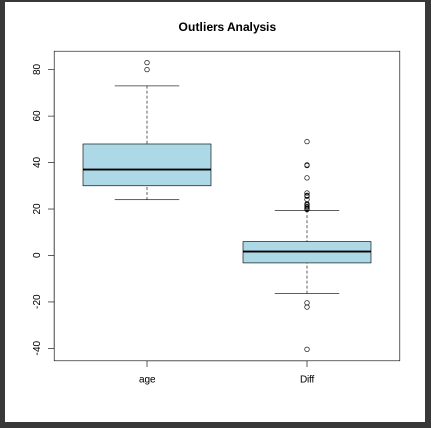
\includegraphics[width=0.5\linewidth]{part01_figures/1.png}
                    \caption{Visualize các biến `Age` và `Diff`}
                    \label{fig:Visualize các biến `Age` và `Diff`}
                \end{figure}
                Từ biểu đồ hộp, ta có nhận xét sau đây:
                    \begin{itemize}
                        \item \textbf{age}: Có một vài điểm cực ngoại lại ở phía trên.
                        \item \textbf{Diff}: Tồn tại nhiều điểm cực ngoại lai ở trên và ở phía dưới box.
                    \end{itemize}
        \end{itemize}
    \item [\textbf{Bước 4}]: \textbf{Trực quan hóa dữ liệu và rút ra nhận xét.}
    
        Ta sẽ dùng R để vẽ ra biểu đồ phân bố chuẩn của dữ liệu
        \begin{lstlisting}
# Biến Age
ggplot(islander_raw, aes(x = age)) +
  geom_histogram(aes(y = ..density..), bins = 30, color = "black", fill = "lightblue") +
  geom_density(alpha = 0.2, fill = "#FF6666") +
  stat_function(fun = dnorm, args = list(mean = mean(islander_raw$age, na.rm = TRUE), sd = sd(islander_raw$age, na.rm = TRUE)),
                color = "blue", size = 1) +
  theme_minimal() +
  labs(title = "Histogram of age variable", x = "age", y = "Density")

  # Biến Diff
  ggplot(islander_raw, aes(x = age)) +
  geom_histogram(aes(y = ..density..), bins = 30, color = "black", fill = "lightblue") +
  geom_density(alpha = 0.2, fill = "#FF6666") +
  stat_function(fun = dnorm, args = list(mean = mean(islander_raw$age, na.rm = TRUE), sd = sd(islander_raw$age, na.rm = TRUE)),
                color = "blue", size = 1) +
  theme_minimal() +
  labs(title = "Histogram of age variable", x = "age", y = "Density")
        \end{lstlisting}
            \begin{figure}[H]
                \centering
                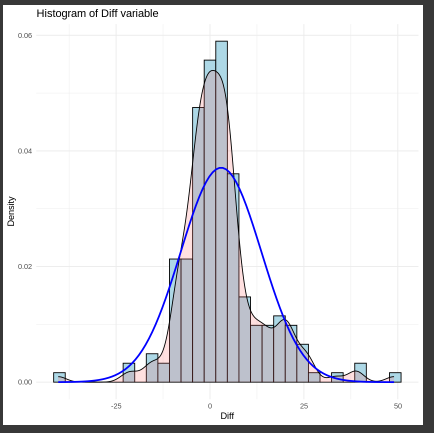
\includegraphics[width=0.3\linewidth]{part01_figures/2.png}
                \caption{Đồ thị phân phối chuẩn của biến `Diff`}
                \label{fig:Đồ thị phân phối chuẩn của biến `Diff`}
            \end{figure}
            \begin{figure}[H]
                \centering
                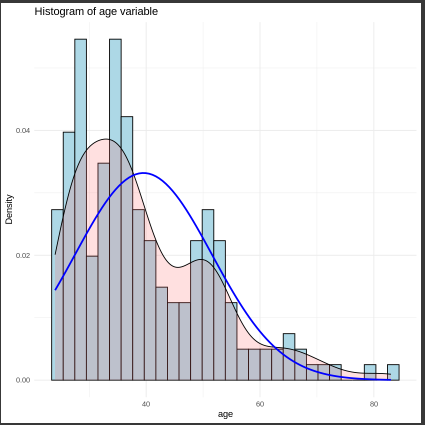
\includegraphics[width=0.3\linewidth]{part01_figures/3.png}
                \caption{Đồ thị phân phối chuẩn của biến `Age`}
                \label{fig:Đồ thị phân phối chuẩn của biến `Age`}
            \end{figure}
        Từ hai đồ thị trên, ta có một số nhận xét như sau:
            - `Age`: Không có dạng phân bố chuẩn, lệch trái so với giá trị trung bình
            - `Diff`: Có dạng phân bố gần chuẩn.
    \item [\textbf{Bước 4}]: \textbf{Kết luận}
    
    Sau khi hoàn thành bước khảo sát dữ liệu, ta có một số kết luận như sau
    \begin{itemize}
        \item [-] Các biến first-name và last-name chứa thông tin về tên của người khảo sát (kiểu dữ liệu character), về mặt thống kê biến này không có ý nghĩa nên sẽ được loại bỏ khỏi dữ liệu khi khảo sát.
        \item[-]  Vì Diff = Mem-Score-Before - Mem-Score-After (đa cộng tuyến), vì vậy ta chỉ cần khảo sát biến phụ thuộc Diff, các biến còn lại sẽ loại bỏ ra khỏi dữ liệu trước khi khảo sát.
        \item[-] Trên thực tế, việc khảo sát trên từng mức nhóm tuổi trải rộng từ 24 đến 83 rất nhiều, ta sẽ tiến hành chia thành 2 nhóm chính là nhóm tuổi < 50 và nhóm còn lại.
        \item[-] Biến phụ thuộc là `Diff` và các biến độc lập bao gồm  HappySadgroup, Dosage, Drug và age. 
    \end{itemize}
\end{itemize}

\subsection{Xử lý dữ liệu}
Ở bước này, chúng ta sẽ tiến hành các bước sau:
\begin{itemize}
    \item [1.] Loai bỏ các biến dư thừa và đưa dữ liệu về dạng thích hợp
    \item [2.] Xây dựng mô hình AOV để xem xét sự phụ thuộc của biến phụ thuộc vào các biến độc lập. Từ đó chọn ra các biến phù hợp để phân tích.
    \item [3.] Visualize các biến cần phân tích theo nhóm và rút ra nhận xét.
\end{itemize}
Sau đây là chi tiết các bước:
\begin{itemize}
    \item \textbf{Bước 1: Loại bỏ các biến cần thiết và asFactor các biến dạng category về dạng factor}

    \begin{lstlisting}
# Remove unesscessary variables
processed_islander = islander_raw[, !(names(islander_raw) %in% c("first_name", "last_name", "Mem_Score_Before", "Mem_Score_After"))]

processed_islander$age = processed_islander$age >= 50
processed_islander$age = factor(processed_islander$age)
processed_islander$Dosage = factor(processed_islander$Dosage)
processed_islander$Drug = factor(processed_islander$Drug)
processed_islander$Happy_Sad_group = factor(processed_islander$Happy_Sad_group)
levels(processed_islander$age)
levels(processed_islander$Drug)
levels(processed_islander$Dosage)
levels(processed_islander$Happy_Sad_group)
    \end{lstlisting}

    Kết quả thu được như sau:
\newpage
\begin{lstlisting}
'FALSE''TRUE'
'A''S''T'
'1''2''3'
'H''S'
\end{lstlisting}

    Kết quả cho ta thấy rằng nhóm tuổi đưọc chia thành 2 nhóm là trước 50 tuổi và từ 50 tuổi trở về sau, có 3 nhóm thuốc là A, S, T; có 3 liều lượng thuốc được sử dụng là 1, 2, 3 tương ứng với thấp, trung bình và cao; số người khảo sát nằm trong 2 nhóm là Happy và Sad (H, S).  


\item \textbf{Bước 2: Xây dựng mô hình AOV để xem xét sự phụ thuộc của biến phụ thuộc vào các biến độc lập như thế nào}
    \begin{lstlisting}
diff_aov = aov(Diff~., data = processed_islander)
summary(diff_aov)
    \end{lstlisting}

    Kết quả
    \begin{lstlisting}
                Df Sum Sq Mean Sq F value   Pr(>F)    
age               1      2     2.1   0.024  0.87821    
Happy_Sad_group   1     11    10.6   0.117  0.73233    
Dosage            2   1222   610.8   6.787  0.00142 ** 
Drug              2   4361  2180.6  24.229 4.19e-10 ***
Residuals       191  17190    90.0                     
---
Signif. codes:  0 '***' 0.001 '**' 0.01 '*' 0.05 '.' 0.1 ' ' 1
    \end{lstlisting}
    Nhìn vào bảng kết quả, ta thấy rằng thực tế các biến `HappySadgroup` và `age` không tham gia vào quá trình giải thích ý nghĩa của biến phụ thuộc `Diff` (với mức ý nghĩa 5\%). Do đó, ta chỉ chọn 2 biến `Drug` và `Dosage` để tiến hành khảo sát. Vậy:
    
    - \textbf{Mục tiêu}: Khảo sát về tác dụng phụ của các loại thuốc chống trầm cảm đối với trí nhớ của người tham gia thử nghiệm, được đánh giá thông qua thời gian hoàn thành một bài kiểm tra trí nhớ

    - \textbf{Biến phản hồi}: `Diff` cho biết chênh lệch giữa thời gian (giây) hoàn thành bài kiểm tra trước và sau khi sử dụng thuốc.
    
    - \textbf{Biến nhân tố}: \textbf{Drug}: Gồm 3 nhóm `A` (Alprazolam), `S` (Placebo) và `T` (Triazolam) và \textbf{Dosage}: Gồm 3 nhóm `1` (thấp), `2` (trung bình) và `3` (Cao)

    \item \textbf{Bước 3: Visualize dữ liệu của các biến theo từng nhóm}
    \begin{lstlisting}
processed_islander = processed_islander[, !(names(processed_islander) %in% c("age", "Happy_Sad_group"))]
# Dosage variable
ggplot(processed_islander ,aes(x=Dosage, y=Diff, colour=Dosage, fill=Dosage))+
  geom_jitter(width=0.25)+
  geom_boxplot(alpha=0.25, outlier.alpha=0) +
  stat_summary(fun.y=mean, colour="black", geom="point",
               shape=18, size=3,show.legend = FALSE) +
  theme_classic() +
  theme(legend.position="none")+
  theme(axis.text = element_text(angle=30, hjust=1, vjust=1))

#  Drug variable
ggplot(processed_islander ,aes(x=Drug, y=Diff, colour=Drug,fill=Drug))+
  geom_jitter(width=0.25)+
  geom_boxplot(alpha=0.25, outlier.alpha=0) +
  stat_summary(fun.y=mean, colour="black", geom="point",
               shape=18, size=3,show.legend = FALSE)+
  theme_classic()+
  theme(legend.position="none")+
  theme(axis.text = element_text(angle=30, hjust=1, vjust=1))
    \end{lstlisting}

Kết quả ta thu được như sau:
    \begin{figure}[H]
        \centering
        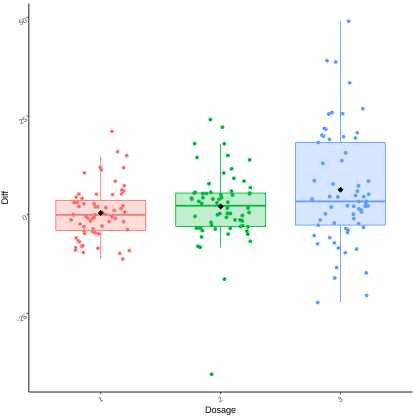
\includegraphics[width=0.4\linewidth]{part01_figures/4.png}
        \caption{Phân phối dữ liệu của từng nhóm Dosage}
        \label{fig:Phân phối dữ liệu của từng nhóm Dosage}
    \end{figure}
    \begin{figure}[H]
        \centering
        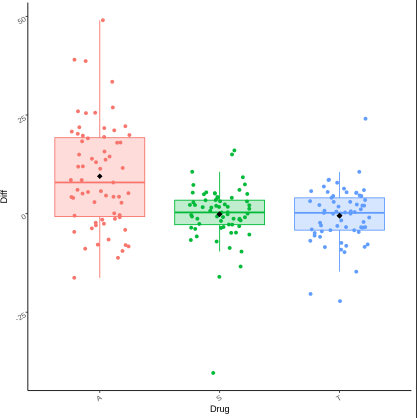
\includegraphics[width=0.4\linewidth]{part01_figures/5.png}
        \caption{Phân phối dữ liệu của từng nhóm Drug}
        \label{fig:Phân phối dữ liệu của từng nhóm Drug}
    \end{figure}

    Nhìn vào đây, ta có thể rút ra một vài nhận xét như sau:
    \begin{itemize}
        \item Đối với Dosage
        \begin{itemize}
            \item Liều lượng thấp: Trung vị Diff gần bằng 0, với phạm vi nhỏ. Hầu hết các điểm dữ liệu tập trung xung quanh trung vị, với một vài ngoại lệ.
            \item Liều lượng trung bình: Trung vị Diff vẫn gần bằng 0, nhưng phạm vi dữ liệu lớn hơn một chút so với liều lượng thấp. Có sự phân bố rộng hơn của các điểm, cho thấy sự biến đổi nhiều hơn trong các phản ứng.
            \item  Liều lượng cao: Trung vị Diff cao hơn so với các nhóm khác, gợi ý rằng liều lượng thuốc này có tác dụng lớn hơn. Có sự biến đổi lớn, với một số điểm nằm khá cao hoặc thấp so với trung vị.IQR lớn hơn và sự hiện diện của các ngoại lệ cho thấy một phạm vi rộng của các phản ứng đối với liều lượng cao.
        \end{itemize}
        Ta rút ra kết luận như sau:
            \begin{itemize}
                \item Biểu đồ gợi ý rằng liều lượng cao hơn có thể có tác động đáng kể hơn đến thời gian hoàn thành bài kiểm tra trí nhớ, được chỉ ra bởi trung vị cao hơn và sự biến đổi lớn hơn trong Diff.
                \item Liều lượng thấp và trung bình cho thấy sự thay đổi nhỏ hơn và ít biến đổi hơn, với nhiều người tham gia có ít hoặc không thay đổi trong thời gian hoàn thành.
                \item Sự phân bố rộng hơn và trung vị cao hơn trong nhóm liều lượng cao có thể cho thấy rằng mặc dù một số người tham gia có lợi ích đáng kể, những người khác có thể gặp tác dụng phụ, dẫn đến phản ứng không tốt.

            \end{itemize}
        \item  Đối với Drug
        \begin{itemize}
            \item Alprazolam (A):Trung vị Diff khá xa với điểm 0 hơn các loại thuốc khác.Có nhiều điểm ngoại lệ, đặc biệt ở phía trên, cho thấy một số người tham gia có sự cải thiện đáng kể về thời gian hoàn thành bài kiểm tra.Trung bình Diff cũng cao hơn, gợi ý rằng Alprazolam có thể có tác dụng tích cực đối với một số người tham gia.

            \item Triazolam (T):Trung vị Diff gần bằng 0, với phạm vi và sự phân tán nhỏ hơn so với Alprazolam. Trung bình Diff gần với trung vị, cho thấy tác dụng của Triazolam ít biến đổi hơn.
            \item Placebo (S):Trung vị Diff gần bằng 0, với phạm vi và sự phân tán tương tự như Triazolam. Có một số điểm ngoại lệ, nhưng không nhiều.Trung bình Diff gần với trung vị, cho thấy tác dụng của giả dược (Placebo) ít biến đổi và không có hiệu quả đáng kể.
        \end{itemize}
        Ta rút ra kết luận như sau:
        \begin{itemize}
            \item Alprazolam (A): Có tác dụng đáng kể đối với một số người tham gia, nhưng cũng có nhiều biến đổi, cho thấy có thể có tác dụng phụ hoặc tác động không đồng nhất.
            \item  Triazolam (T) và Placebo (S): Không có sự thay đổi đáng kể trong thời gian hoàn thành bài kiểm tra, gợi ý rằng các loại thuốc này có ít hoặc không có tác dụng cải thiện trí nhớ.
        \end{itemize}
    \end{itemize}

    Ta xem xét biến phụ thuộc Diff bằng cách xét lại biểu đồ phân bố chuẩn như sau:
    \begin{lstlisting}
ggplot(processed_islander, aes(x = Diff)) +
  geom_histogram(aes(y = ..density..), bins = 30, color = "black", fill = "lightblue") +
  geom_density(alpha = 0.2, fill = "#FF6666") +
  stat_function(fun = dnorm, args = list(mean = mean(processed_islander$Diff, na.rm = TRUE), sd = sd(processed_islander$Diff, na.rm = TRUE)),
                color = "blue", size = 1) +
  theme_minimal() +
  labs(title = "Histogram of Diff variable", x = "Diff", y = "Density")
    \end{lstlisting}
    \begin{figure}[H]
                \centering
                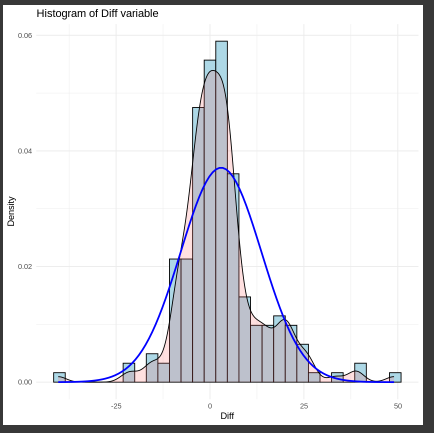
\includegraphics[width=0.8\linewidth]{part01_figures/2.png}
                \caption{Đồ thị phân phối chuẩn của biến `Diff`}
                \label{fig:Đồ thị phân phối chuẩn của biến `Diff`_}
            \end{figure}
    Ta cũng rút ra một vài nhận xét như sau:
    \begin{itemize}
        \item Độ lệch
        \begin{itemize}
            \item Trung bình (Mean) của biến Diff là 2.955, cho thấy thời gian trung bình hoàn thành bài kiểm tra sau khi dùng thuốc tăng thêm khoảng 2.955 giây.
            \item Median (Trung vị) là 1.700, thấp hơn giá trị trung bình, cho thấy sự phân phối không hoàn toàn đối xứng.
        \end{itemize}
        \item Phân Bố Dữ Liệu: Dữ liệu phân bố khá gần với phân phối chuẩn, nhưng có một vài khác biệt:
        \begin{itemize}
            \item Có một sự tập trung dữ liệu khá cao xung quanh giá trị 0 đến 5, tạo nên một đỉnh phân phối cao hơn so với đường chuẩn.
            \item Có sự lan tỏa dữ liệu về cả hai phía của đỉnh, nhưng ít hơn ở phía cực trái (khoảng -40) và cực phải (khoảng 50).
        \end{itemize}

        \item Khoảng Tứ Phân Vị:
        \begin{itemize}
            \item 1st Qu. (Quartile đầu tiên): -3.175.
            \item 3rd Qu. (Quartile thứ ba): 5.925.
            \item Điều này cho thấy phần lớn dữ liệu nằm trong khoảng từ -3.175 đến 5.925, một khoảng phân tán rộng nhưng không đối xứng hoàn toàn quanh trung vị.
        \end{itemize}
        \item  Đỉnh và đuôi: Biểu đồ cho thấy một đỉnh lớn, khá hẹp, và hai đuôi phân phối khá dài, đặc biệt ở phía phải (hơn 25). Điều này chỉ ra rằng có một số giá trị cực đại cao (tăng lớn trong thời gian hoàn thành bài kiểm tra sau khi dùng thuốc).
    \end{itemize}
    \newpage
    Kết Luận:
    \begin{itemize}
        \item Sự Phân Tán và Độ Lệch: Biểu đồ cho thấy sự tăng thời gian hoàn thành bài kiểm tra (Diff) sau khi dùng thuốc là phổ biến, với giá trị trung bình dương. Tuy nhiên, phân phối không hoàn toàn đối xứng, với một số giá trị cực đại ở cả hai phía.
        \item Khả Năng Phân Phối Chuẩn: Phân phối của biến Diff khá gần với phân phối chuẩn, nhưng có một số khác biệt như đỉnh phân phối cao hơn và đuôi phân phối dài hơn. Điều này có thể là do tác động của một số cá nhân phản ứng mạnh mẽ với thuốc hơn so với phần còn lại.
    \end{itemize}
\end{itemize}

\subsection{Kiểm định các giả thiết thống kê (ANOVA assumptions)}
Nhắc lại các điều kiện để phân tích ANOVA như sau:
\begin{itemize}
    \item [1.] Các mẫu độc lập
    \item [2.] Biến phụ thuộc là biến liên tục
    \item [3.] Các nhóm có phân phối chuẩn hoặc gần chuẩn, đồng nghĩa với việc kiểm định phương sai các nhóm cho kết quả là đồng nhất.
\end{itemize}

Rõ ràng, theo như phân tích phía trên, bộ dữ liệu chúng ta đã thỏa mãn điều kiện (1) và (2). Để chắc chắn ta sẽ đi kiểm định yêu cầu số (3) bằng cách tiến hành thực hiện các kiểm định sau:
\begin{itemize}
    \item Shapiro-Wilk test
    \item leveneTest
    \item durbinWatsonTest
\end{itemize}

Đầu tiên ta sẽ xây dựng mô hình tương tác bằng dòng lệnh sau
\begin{lstlisting}
# Xây dựng mô hình tương tác
int_model = aov(Diff~Dosage * Drug, data = processed_islander)
summary(int_model)
\end{lstlisting}

Kết quả thu được:

\begin{lstlisting}
                 Df Sum Sq Mean Sq F value   Pr(>F)    
Dosage        2   1222   610.9   9.536 0.000113 ***
Drug          2   4314  2156.9  33.666 3.12e-13 ***
Dosage:Drug   4   5141  1285.3  20.062 8.74e-14 ***
Residuals   189  12109    64.1                     
---
Signif. codes:  0 '***' 0.001 '**' 0.01 '*' 0.05 '.' 0.1 ' ' 1
\end{lstlisting}
Với mức ý nghĩa 5\%, ta thấy rằng giữa `Dosage` và `Drug` có mối quan hệ tương tác với nhau dẫn đến tác động hiệu quả của việc dùng thuốc đối với trí nhớ của người sử dụng. Tiếp tục đi kiểm định các thông số sau:

\begin{lstlisting}
# Shapiro-Wilk test
int_model = aov(Diff~Dosage * Drug, data = processed_islander)
av_residual = rstandard(int_model)
shapiro.test(av_residual)
# QQ plot
qqnorm(av_residual)
qqline(av_residual)
hist(av_residual)
\end{lstlisting}

\begin{figure}[H]
    \centering
    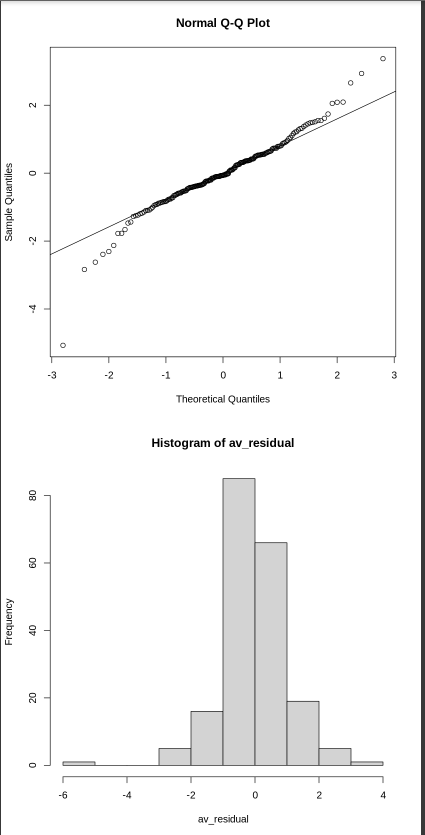
\includegraphics[width=0.45\linewidth]{part01_figures/6.png}
    \caption{Biểu đồ phần dư}
    \label{fig:Biểu đồ phần dư}
\end{figure}

\newpage
Kết quả như sau:
\begin{lstlisting}
    	Shapiro-Wilk normality test

data:  av_residual
W = 0.95575, p-value = 7.794e-06
\end{lstlisting}

Xét giả định
\begin{itemize}
    \item H0: Tuân theo phân phối chuẩn
    \item H1: Không tuân theo phân phối chuẩn
\end{itemize}

Nhận xét: Với độ tin cậy 5\% thì với giá trị p-value = 7.794e-06 chúng ta đủ cơ sở bác bỏ H0, vậy phần dư có phân phối không chuẩn. Nhìn vào biểu đồ, ta thấy rằng ở phần đuôi kéo dài, có một vài điểm bị kéo lệch ra khỏi đường thẳng, điều này chứng tỏ rằng khả năng các điểm nhiễu chính là các điểm ngoại lệ (outliners), tuy nhiên, về mặt tổng quan, dữ liệu vẫn có dạng gần chuẩn, do đó, ta vẫn có thể tiến hành kiểm tra ANOVA. Ở bước cải tiến, ta sẽ tiến hành xử lý các điểm ngoại lệ này để so sánh với kiểm định ban đầu.

Bước tiếp theo ta Kiểm định các nhóm có phương sai đồng nhất hay không
\begin{lstlisting}
leveneTest(int_model)
\end{lstlisting}

Kết quả
\begin{lstlisting}
Df	F value	Pr(>F)
<int>	<dbl>	<dbl>
group	8	0.9961061	0.4404991
189	NA	NA
\end{lstlisting}

Giả định:

- H0: Các nhóm có phương sai đồng nhất

- H1: Các nhóm không có phương sai đồng nhất

Nhận xét: Với giá trị p-value = 0.4404991 > 0.05, ta không đủ điều kiện bác bỏ H0, vậy các nhóm có phương sai đồng nhất. Như vậy, bộ dữ liệu này đã thoả mãn điều kiện yêu cầu để phân tích ANOVA. Tuy nhiên, để hiểu sâu hơn về bộ dữ liệu, ta tiếp tục đi kiểm định tính độc lập của phần dư bằng dòng lệnh sau

\newpage
\begin{lstlisting}
# Kiểm định tính độc lập của phần dư
durbinWatsonTest(int_model)
plot(int_model, 1)
\end{lstlisting}

Kết quả 
\begin{lstlisting}
 lag Autocorrelation D-W Statistic p-value
   1     -0.05315976      2.105716   0.816
 Alternative hypothesis: rho != 0

\end{lstlisting}
\begin{figure}[H]
    \centering
    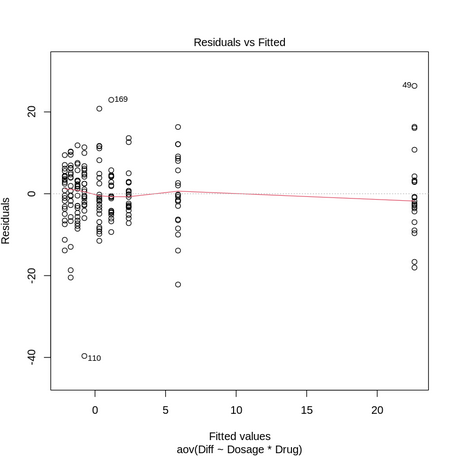
\includegraphics[width=0.8\linewidth]{part01_figures/7.png}
    \caption{Kiểm định độc lập phần dư}
    \label{fig:Kiểm định độc lập phần dư}
\end{figure}
Với giả định:
\begin{itemize}
    \item H0: Không có sự tương quan (độc lập).
    \item H1: H1: Có sự tương quan (không độc lập).
\end{itemize}

Thì với giá trị p-value = 0.816 (> 0.05) nên không có sự tương quan. Vậy phần dư độc lập

\subsection{Phân tích phương sai k nhân tố}
Tiếp theo chung ta sẽ tiến hành đi phân tích phương sai k nhân tố. Việc này gồm các bước sau:
\begin{itemize}
    \item [1.] Kiểm tra sự tương tác
    \item [2.] Phân tích ảnh hưởng đơn
    \begin{itemize}
        \item Phân tích ảnh hưởng đơn của liều lượng ở mỗi loại thuốc
        \item Phân tích ảnh hưởng đơn của thuốc ở mỗi liều lượng
    \end{itemize}
    \item [3.] Phân tích ảnh hưởng chính
    \begin{itemize}
        \item Phân tích ảnh hưởng chính của Dosage với hiệu quả của bài kiểm tra trí nhớ
        \item Phân tích ảnh hưởng chính của Drug với hiệu quả của bài kiểm tra trí nhớ
    \end{itemize}
\end{itemize}

Sau đây là các bước chi tiết:
\begin{itemize}
    \item \textbf{Bước 1: Xây dựng mô hình tương tác (interaction model) và kiểm tra tương tác của các biến}

    \begin{lstlisting}
    int_model = aov(Diff~Dosage * Drug, data = processed_islander)
    summary(int_model)
    plot(interactionMeans(int_model))
    \end{lstlisting}

    Kết quả
    \begin{lstlisting}
                     Df Sum Sq Mean Sq F value   Pr(>F)    
Dosage        2   1222   610.9   9.536 0.000113 ***
Drug          2   4314  2156.9  33.666 3.12e-13 ***
Dosage:Drug   4   5141  1285.3  20.062 8.74e-14 ***
Residuals   189  12109    64.1                     
---
Signif. codes:  0 '***' 0.001 '**' 0.01 '*' 0.05 '.' 0.1 ' ' 1
    \end{lstlisting}
Ta rút ra một số nhận xét dựa trên kết quả như sau: 

- Với mức ý nghĩa 5\%, ta thấy giữa `Dosage` và `Drug` có sự tương tác với nhau (p-value=8.74e-14). Sự kết hợp giữa hàm lượng thuốc và loại thuốc có ảnh hưởng rất lớn đến thời gian hoàn thành bài kiểm tra, cho thấy rằng không chỉ từng yếu tố riêng lẻ mà sự kết hợp giữa chúng cũng rất quan trọng.

- Đối với biểu đồ bên trái: Biểu đồ bên trái biểu diễn sự tương tác giữa Dosage và Drug dựa trên giá trị trung bình điều chỉnh của Diff.
    \begin{itemize}
        \item [+]  Đồ thị trên cùng bên trái (Dosage theo Drug):
        \begin{itemize}
            \item Cho thấy sự thay đổi của Diff theo liều lượng (Dosage) cho từng loại thuốc (Drug).
            \item Đối với tất cả các loại thuốc, Diff tăng dần khi tăng liều lượng từ 1 đến 3.
        \end{itemize}
        \item [+]  Đồ thị dưới cùng bên trái (Drug theo Dosage):
        \begin{itemize}
            \item Cho thấy sự thay đổi của Diff theo loại thuốc (Drug) cho từng liều lượng (Dosage).
            \item Khi liều lượng là 1: sự khác biệt giữa các loại thuốc là tương đối nhỏ. Trong đó loại S cho hiệu quả cao nhất, A và T cho kết quả tệ hơn trước khi sử dụng (mean < 0).
            \item Khi liều là 2: Có sự thay đổi rõ rệt ở các loại thuốc: Loại S cho kết quả tệ hơn so với trước khi dùng thuốc, loại T có hiệu quả không đáng kể, loại A cho thấy hiệu quả vượt bật.
            \item Khi liều lượng là 3: Sự khác biệt giữa các loại thuốc trở nên rõ rệt hơn, với Thuốc A cho kết quả tốt nhất so với 3 loại và ở cả 3 liều lượng, trong khi 2 loại còn lại cho kết quả tệ hơn trước khi dùng.
        \end{itemize}
    \end{itemize}

- Đối với biểu đồ bên phải: Biểu đồ bên phải biểu diễn sự tương tác giữa Drug và Dosage dựa trên giá trị trung bình điều chỉnh của Diff.
    \begin{itemize}
        \item [+] Đồ thị trên cùng bên phải (Drug theo Dosage):
        \begin{itemize}
            \item Tương tự như đồ thị dưới cùng bên trái của biểu đồ bên trái, nhưng theo chiều ngược lại. Cho thấy sự thay đổi của Diff theo loại thuốc cho từng liều lượng.
            \item Đối với thuốc A: Cho kết quả tốt liều lượng cao và trung bình, liều lượng thấp không có sự thay đổi
            \item Đối với thuốc T: Không có sự khác biệt giữa các liều lượng và hiệu quả sau và trước khi sửng dụng (Thậm chí giảm (tệ))
            \item Đối với thuốc S: Giống T
        \end{itemize}
        \item [+] Đồ thị dưới cùng bên phải (Dosage theo Drug):
        \begin{itemize}
            \item Tương tự như đồ thị trên cùng bên trái của biểu đồ bên trái, nhưng theo chiều ngược lại.
            \item Cho thấy sự thay đổi của Diff theo liều lượng cho từng loại thuốc.
            \item Cơ bản các thuốc cho kết quả tốt nhất theo thứ tự là là A > S > T.
        \end{itemize}
    \end{itemize}
Ta có kết luận sau đây:
    \begin{itemize}
        \item Cả liều lượng và loại thuốc đều có ảnh hưởng đáng kể đến Diff.
        \item Có sự tương tác đáng kể giữa liều lượng và loại thuốc, nghĩa là hiệu quả của liều lượng khác nhau phụ thuộc vào loại thuốc được sử dụng.
        \item Biểu đồ cho thấy rõ ràng rằng Thuốc A (Alprazolam) có ảnh hưởng lớn nhất khi liều lượng tăng, trong khi S có ảnh hưởng ít nhất.
    \end{itemize}

\item \textbf{Bước 2: Phân tích ảnh hưởng đơn}

        Để phân tích ảnh hưởng đơn ta sẽ sử dụng hàm \textbf{testInteractions} để tiến hành phân tích. Sau đây là các bước chi tiết
    \begin{itemize}
        \item Phân tích ảnh hưởng đơn của liều lượng ở mỗi loại thuốc
            \begin{lstlisting}
testInteractions(int_model, fixed = "Drug", across = "Dosage")
            \end{lstlisting}
            Kết quả:
            \begin{figure}[H]
                \centering
                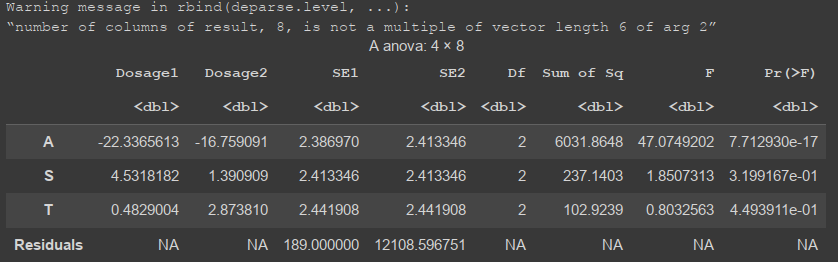
\includegraphics[width=0.8\linewidth]{part01_figures/8.png}
                \caption{Kết quả ảnh hưởng đơn giữa Drug và Dosage}
                \label{fig:Kết quả ảnh hưởng đơn giữa Drug và Dosage}
            \end{figure}
            Với các giả định như sau:
            \begin{itemize}
                \item H0: Liều lượng không ảnh hưởng đến hiệu quả thuốc
                \item H1: Liều lượng có ảnh hưởng đến hiệu quả của thuốc
            \end{itemize}
            Ta rút ra kết luận như sau: Với kết quả phân tích ta có một số nhận xét như sau, với độ tin cậy 5\% thì:
            \begin{itemize}
                \item Liều lượng có ảnh hưởng đến kết quả của loại thuốc A
                \item Liều lượng không ảnh hưởng đến kết quả của lọa thuốc S và T
            \end{itemize}
        \item Phân tích ảnh hưởng đơn của thuốc ở mỗi liều lượng
            \begin{lstlisting}
    testInteractions(int_model, fixed = "Dosage", across = "Drug")
            \end{lstlisting}
            \begin{figure}[H]
                \centering
                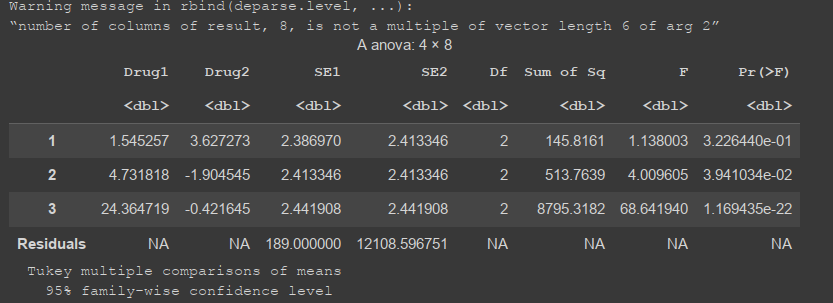
\includegraphics[width=0.8\linewidth]{part01_figures/9.png}
                \caption{Ảnh hưởng đơn giữa Drug và Dosage.}
                \label{fig:Ảnh hưởng đơn giữa Drug và Dosage.}
            \end{figure}
            Tương tự như ở phía trên, ta có các giả định như sau:
            \begin{itemize}
                \item H0: Các loại thuốc sẽ không tác động ở mỗi liều lượng
                \item H1: Các loại thuốc sẽ có tác động ở mỗi liều lượng
            \end{itemize}
        Ta rút ra kết luận như sau: Với kết quả phân tích ta có một số nhận xét như sau, với độ tin cậy 5\% thì:
            \begin{itemize}
                \item Hầu hết các loại thuốc sẽ có tác động ở liều lượng cao
                \item Liều lượng trung bình cũng sẽ có tác động nhưng không đáng kể (có ý nghĩa ở mức 0.4%)
                \item Liều lượng thấp cho kết quả không đáng kể.
            \end{itemize}
        \item Phân tích ảnh hưởng đơn giữa các nhóm thuốc ứng với mỗi liều lượng
        
        Việc phân tích sự tương tác của các nhóm trong cùng một liều lượng cũng có ý nghĩa rất quan trọng trong thống kê, từ đó sẽ hiểu rõ hơn về từng tác dụng của từng loại và từng nhóm
        \begin{lstlisting}
options(contrasts = c(unordered="contr.sum", ordered="contr.poly"))
A_vs_S = list(Drug = c(1, -1, 0))
A_vs_T = list(Drug = c(1, 0, -1))
S_vs_T = list(Drug = c(0, 1, -1))
        \end{lstlisting}

        Đầu tiên, ta sẽ đi phân tích ảnh hưởng của nhóm A và S
        \begin{lstlisting}
testInteractions(int_model, custom = c(A_vs_S), fixed = "Dosage", adjustment = "bonferroni")
        \end{lstlisting}
        Kết quả:
        \begin{figure}[H]
            \centering
            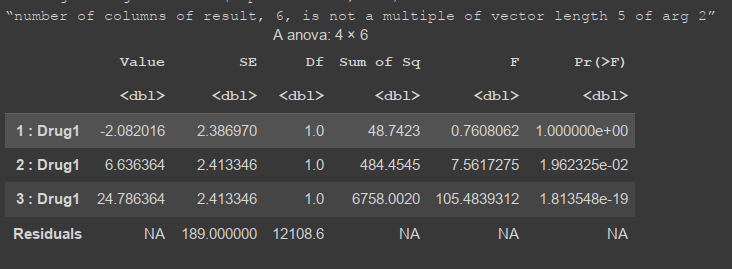
\includegraphics[width=0.8\linewidth]{part01_figures/10.png}
            \caption{Tương tác giữa nhóm A và S ở mỗi liều lượng}
            \label{fig:Tương tác giữa nhóm A và S ở mỗi liều lượng}
        \end{figure}
        Ta có giả định như sau:
        \begin{itemize}
            \item Không có sự khác nhau giữa nhóm thuốc A và S ở các liều lượng
            \item Có sự khác nhau giữa nhóm thuốc A và S ở các liều lượng
        \end{itemize}
        Ta rút ra kết luận như sau: Với kết quả phân tích ta có một số nhận xét như sau, với độ tin cậy 5\% thì:
        \begin{itemize}
            \item Có sự khác biệt về hiệu quả khi sử dụng thuốc thuốc A và S ở các  liều lượng cao và trung bình
            \item Ở liều lượng thấp: Không có sự khác biệt
        \end{itemize}

        Tiếp theo là nhóm A và T
        
        \begin{lstlisting}
testInteractions(int_model, custom = c(A_vs_T), fixed = "Dosage", adjustment = "bonferroni")
        \end{lstlisting}
        Kết quả:
        \begin{figure}[H]
            \centering
            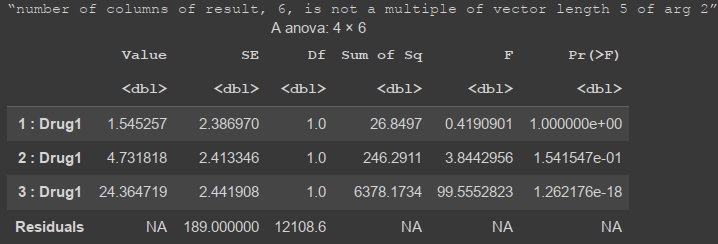
\includegraphics[width=0.8\linewidth]{part01_figures/11.png}
            \caption{Tương tác giữa nhóm A và T ở mỗi liều lượng}
            \label{fig:Tương tác giữa nhóm A và T ở mỗi liều lượng}
        \end{figure}
        Với các giả định tương tự với nhóm A và S, ta có kết luận như sau:
        \begin{itemize}
            \item Ở liều cao: Có sự khác biệt về hiệu quả khi sử dụng thuốc ở các  loại thuốc A và T
            \item Ở liều thấp và trung bình: Không có sựu ảnh hưởng rõ rệt
        \end{itemize}
        Cuối cùng là giữa nhóm S và T
        \begin{lstlisting}
testInteractions(int_model, custom = c(S_vs_T), fixed = "Dosage", adjustment = "bonferroni")
        \end{lstlisting}
        Kết quả:
        \begin{figure}[H]
            \centering
            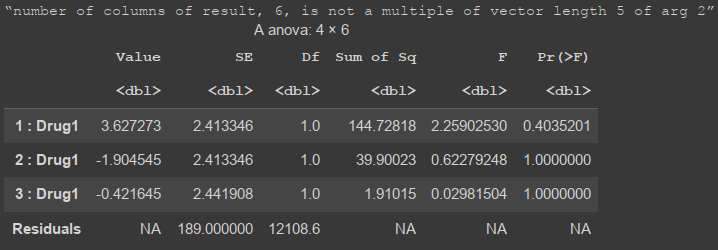
\includegraphics[width=0.8\linewidth]{part01_figures/12.png}
            \caption{Tương tác giữa nhóm S và T ở mỗi liều lượng}
            \label{fig:Tương tác giữa nhóm S và T ở mỗi liều lượng}
        \end{figure}
         Với các giả định tương tự với nhóm A và S, ta có kết luận như sau: Với độ tin cậy 5\% thì không có sự khác biệt nào ở cả 3 liều lượng.
    \end{itemize}
    Từ việc phân tích trên, ta có kết luận như sau: Khi dùng thuốc liều cao, giữa các nhóm sẽ cho ra các phản ứng ảnh hưởng đến trí nhớ ở nhóm A-T và A-S. Tuy nhiên, nhóm S-T lại không cho thấy sự tương tác nào có ý nghĩa thống kê.

    \item Phân tích ảnh hưởng đơn giữa các nhóm liều lượng ứng với mỗi loại thuốc
    Tương tự cho trường hợp \textbf{Phân tích ảnh hưởng đơn giữa các nhóm thuốc ứng với mỗi liều lượng}, ta cũng phân tích ảnh hưởng đơn giữa các nhóm liều lượng ứng với mỗi loại thuốc như thế nào
    \begin{lstlisting}
options(contrasts = c(unordered="contr.sum", ordered="contr.poly"))
low_vs_medium = list(Dosage = c(1, -1, 0))
low_vs_high = list(Dosage = c(1, 0, -1))
medium_vs_high = list(Dosage = c(0, 1, -1))
    \end{lstlisting}
    Đầu tiên là nhóm thấp và trung bình
    \begin{lstlisting}
# Nhóm thấp và trung bình
testInteractions(int_model, custom = c(low_vs_medium), fixed = "Drug", adjustment = "bonferroni")
    \end{lstlisting}
    Kết quả:
    \begin{figure}[H]
        \centering
        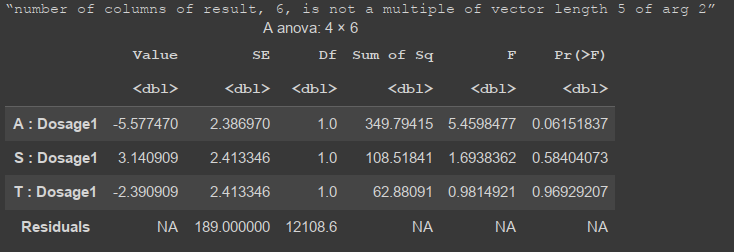
\includegraphics[width=0.8\linewidth]{part01_figures/13.png}
        \caption{Tương tác giữa nhóm thấp và nhóm trung bình}
        \label{fig:Tương tác giữa nhóm thấp và nhóm trung bình}
    \end{figure}
    Với giả định sau:
        \begin{itemize}
            \item H0: Không có sự tương tác nhau giữa liều thấp và liều trung bình ở loại thuốc X (A, T, S)
            \item H1: Có sự tương tác nhau giữa liều thấp và liều trung bình ở  ở loại thuốc X (A, T, S)
        \end{itemize}
    Với độ tin cậy 5\% thì
    \begin{itemize}
        \item Ở loại thuốc A: Có sự tương tác về hiệu quả khi sử dụng thuốc ở các  liều lượng thấp và liều lượng trung bình
        \item Ở loại thuốc S và T: Không có sự tương tác
    \end{itemize}

    Tiếp theo là nhóm thấp và cao
    \begin{lstlisting}
# Nhóm thấp và cao
testInteractions(int_model, custom = c(low_vs_high), fixed = "Drug", adjustment = "none")
    \end{lstlisting}
\begin{figure}[H]
    \centering
    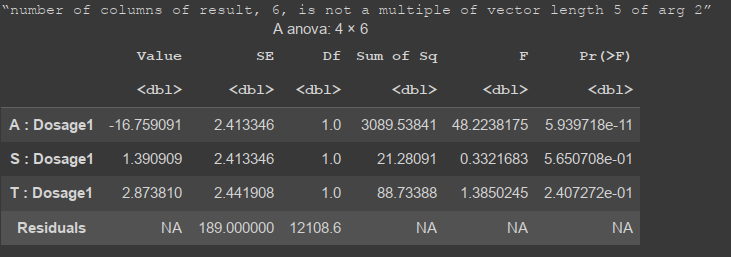
\includegraphics[width=0.8\linewidth]{part01_figures/14.png}
    \caption{Tương tác giữa nhóm thấp và cao}
    \label{fig:Tương tác giữa nhóm thấp và cao}
\end{figure}
    Tương tự như trên ta rút ra nhận xét như sau: Với mức ý nghĩa 5\%
    \begin{itemize}
        \item Ở loại thuốc A: Có sự tương tác khi sử dụng thuốc ở các liều lượng thấp và liều lượng cao
        \item Ở loại thuốc S và T: Không có sự tương tác mang ý nghĩ thống kê
    \end{itemize}

    Cuối cùng là nhóm trung bình và cao
    \begin{lstlisting}
# Nhóm trung bình và cao
testInteractions(int_model, custom = c(medium_vs_high), fixed = "Drug", adjustment = "none")
    \end{lstlisting}
\begin{figure}[H]
    \centering
    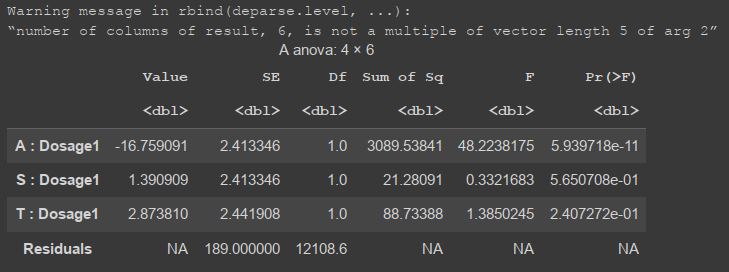
\includegraphics[width=0.8\linewidth]{part01_figures/15.png}
    \caption{Tương tác giữa nhóm trung bình và cao}
    \label{fig:Tương tác giữa nhóm trung bình và cao}
\end{figure}
    Tương tự như trên ta rút ra nhận xét như sau: Với mức ý nghĩa 5\%
    \begin{itemize}
        \item Có sự tương tác khi sử dụng thuốc ở các  liều lượng trung bình và liều lượng cao
        \item Không có sự tương tác mang ý nghĩa thống kê
    \end{itemize}

    Qua việc phân tích trên ta có một số kết luận như sau:
    \begin{itemize}
        \item Hầu hết các liều lượng thấp và trung bình sẽ cho thấy mức độ ít tương tác mang ý nghĩ thống kê ở các loại thuốc
        \item Hầu hết các loại thuốc T và S cho kết quả là không có sự tương tác giữa liều lượng với loại A
    \end{itemize}
    \item \textbf{Bước 3: Phân tích ảnh hưởng chính}

    Ở bước này ta sẽ thực hiện 2 phân tích:
    \begin{itemize}
        \item Phân tích ảnh hưởng chính của Dosage với hiệu quả của bài kiểm tra trí nhớ
        \item Phân tích ảnh hưởng chính của Drug với hiệu quả của bài kiểm tra trí nhớ
    \end{itemize}
    Với mỗi bước, ta sẽ thực hiện các công việc sau:
    \begin{itemize}
        \item Xây dựng mô hình
        \item Kiểm định các giả thiết của mô hình
        \item Kiểm định trung bình của các nhóm
        \item Nhận xét
    \end{itemize}
    Sau đây là các bước phân tích cụ thể:
    \begin{itemize}
        \item \textbf{Bước 3.1: Phân tích ảnh hưởng chính của Dosage với hiệu quả của bài kiểm tra trí nhớ}
        \begin{lstlisting}
dosage_model = aov(Diff~Dosage, data = processed_islander)
summary(dosage_model)
        \end{lstlisting}
        Kết quả:
        \begin{lstlisting}
            Df Sum Sq Mean Sq F value  Pr(>F)   
Dosage        2   1222   610.9   5.524 0.00464 **
Residuals   195  21563   110.6                   
---
Signif. codes:  0 '***' 0.001 '**' 0.01 '*' 0.05 '.' 0.1 ' ' 1
        \end{lstlisting}
        Nhận xét: Với mức ý nghĩa 0.05, ta thấy rằng Dosage có ý nghĩa trong việc giải thích mô hình

        Tiếp theo tiến hành kiểm định các giả thuyết
        \begin{lstlisting}
# Shapiro-Wilk test
av_residual = rstandard(dosage_model)
shapiro.test(av_residual)

# Trực quan bằng QQ plot
qqnorm(av_residual)
qqline(av_residual)
hist(av_residual)
        \end{lstlisting}
        Kết quả:
        \begin{lstlisting}
    Shapiro-Wilk normality test

data:  av_residual
W = 0.94813, p-value = 1.397e-06
        \end{lstlisting}
        Với giả định:
        \begin{itemize}
            \item H0: Phần dư Tuân theo phân phối chuẩn.
            \item H1: Phần dư Không tuân theo phân phối chuẩn.
        \end{itemize}
        Như vậy với độ tin cậy 5\% thì với giá trị p-value = 1.397e-06 chúng ta đủ cơ sở bác bỏ H0, vậy sai số có phân phối không chuẩn. Nhìn vào biểu đồ, ta thấy rằng ở phần đuôi kéo dài, có một vài điểm bị kéo lệch ra khỏi đường thẳng --> Khả năng các điểm nhiễu chính là các điểm ngoại lệ (outliners), tuy nhiên, về mặt tổng quan, dữ liệu vẫn có dạng gần chuẩn.

    \begin{lstlisting}
# Kiểm định các nhóm có phương sai đồng nhất hay không
leveneTest(dosage_model)
    \end{lstlisting}
    Kết quả:
    \begin{lstlisting}
        A anova: 2 x 3 	
        Df	F value	Pr(>F)
	<int>	<dbl>	  <dbl>
group	2	11.76277   1.502826e-05
	   195	       NA	       NA
    \end{lstlisting}
    Với giả định:
    \begin{itemize}
        \item Các nhóm có phương sai đồng nhất.
        \item Các nhóm không có phương sai đồng nhất.
    \end{itemize}
    Nhận xét: Với giá trị p-value = 1.502826e-05 < 0.05, ta đủ điều kiện bác bỏ H0, vậy các nhóm có phương sai không đồng nhất.
    \end{itemize}
    \begin{lstlisting}
# Kiểm định tính độc lập của phần dư
durbinWatsonTest(dosage_model)
plot(dosage_model, 1)
    \end{lstlisting}
    Kết quả:
    \begin{lstlisting}
 lag Autocorrelation D-W Statistic p-value
   1       0.3993242      1.198467       0
 Alternative hypothesis: rho != 0        
    \end{lstlisting}
    Với giả định:
    \begin{itemize}
        \item H0: Không có sự tương quan (độc lập)
        \item H1: Có sự tương quan (không độc lập)
    \end{itemize}
    Nhận xét: Với giá trị p-value = 0 nên có sự tương quan dương.

Măc dù với điều kiện phương sai giữa các nhóm không đồng nhất nên sẽ không tiến hành phân tích ANOVA được, tuy nhiên về mặc trực quan hóa dữ liệu, ta thấy rằng đồ thị phân bố dạng gần chuẩn, nên ta sẽ tiếp tục đi phân tích các yếu tố ANOVA.
\newpage

    \begin{lstlisting}
# Kiểm định trung bình giữa các nhóm liều lượng
with(processed_islander, pairwise.t.test(Diff, Dosage, p.adj = "bonferroni"))
TukeyHSD(aov(Diff~Dosage, data=processed_islander), conf.level = 0.95)
plot(TukeyHSD(aov(Diff~Dosage, data=processed_islander), conf.level = 0.95))
    \end{lstlisting}
    Kết quả:
    \begin{lstlisting}

	Pairwise comparisons using t tests with pooled SD 

data:  Diff and Dosage 

  1      2     
2 1.0000 -     
3 0.0045 0.0620

P value adjustment method: bonferroni 

  Tukey multiple comparisons of means
    95% family-wise confidence level

Fit: aov(formula = Diff ~ Dosage, data = processed_islander)

$Dosage
        diff         lwr       upr     p adj
2-1 1.611827 -2.69534819  5.919003 0.6511582
3-1 5.899403  1.57556917 10.223237 0.0042357
3-2 4.287576 -0.05235809  8.627510 0.0536311        
    \end{lstlisting}
    Với giả định:
    \begin{itemize}
        \item H0: Các giá trị trung bình giữa các cặp bằng nhau
        \item H1: Các giá trị trung bình giữa các cặp không bằng nhau
    \end{itemize}
    Nhìn vào kết quả ta có: Cặp 3-1 có p-value đều có giá trị nhỏ hơn 0.05 (độ tin cậy 95\%) nên ta cơ sở để bác bỏ H0. Vậy rõ ràng giữa các nhóm này có giá trị trung bình là khác nhau. Nghĩa là các nhóm thuốc liều cao và thấp thì cho thấy mức độ ảnh hưởng đến bệnh nhân khác nhau. Còn các nhóm còn lại thì không, Để rõ hơn, nhìn vào kết quả và hình vẽ ta cũng thấy ngay giữa nhóm 3-1 có mức độ hiệu quả trung bình khác nhau, 3-2 và 1-2 có mức độ hiệu quả trung bình như nhau (đồ thị cắt điểm 0).

    \begin{lstlisting}
# Phân tích tương tác của từng nhóm liều lượng với nhau
A_vs_S = list(Dosage = c(1, -1, 0))
A_vs_T = list(Dosage = c(1, 0, -1))
S_vs_T = list(Dosage = c(0, 1, -1))
testInteractions(dosage_model, custom = A_vs_S, adjustment = 'bonferroni')
print("----------------------------------------------------------")
testInteractions(dosage_model, custom = A_vs_T, adjustment = 'bonferroni')
print("----------------------------------------------------------")
testInteractions(dosage_model, custom = S_vs_T, adjustment = 'bonferroni')
    \end{lstlisting}
Kết quả
\begin{figure}[H]
    \centering
    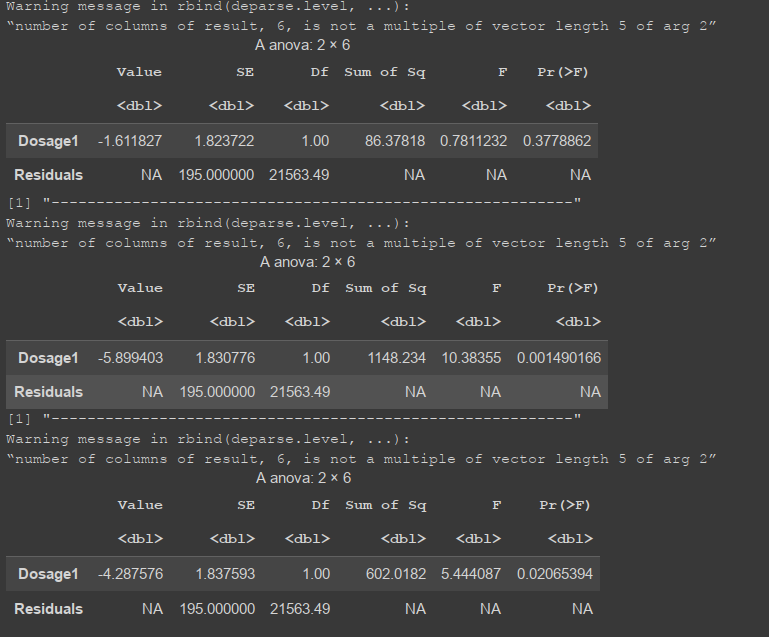
\includegraphics[width=0.8\linewidth]{part01_figures/16.png}
    \caption{Phân tích t-test các nhóm}
    \label{fig:Phân tích t-test các nhóm}
\end{figure}
Với các giả định:
    \begin{itemize}
        \item H0: Không có sự tương tác giữa 2 nhóm thuốc được nhắc đến.
        \item H1: H1: Có sự tương tác giữa 2 nhóm thuốc được nhắc đến
    \end{itemize}
    Với độ tin cậy 0.05, ta có nhận xét như sau:
    \begin{itemize}
        \item Nhóm A và S không có sự tương tác với nhau
        \item Nhóm A và T có sự tương tác với nhau
        \item Nhóm T và S có sự tương tác với nhau
    \end{itemize}

\item \textbf{Bước 3.2: Phân tích ảnh hưởng chính của Drug với hiệu quả của bài kiểm tra trí nhớ}
    \begin{lstlisting}
drug_model = aov(Diff~Drug, data = processed_islander)
summary(drug_model)
    \end{lstlisting}

\newpage
Kết quả:
    \begin{lstlisting}
             Df Sum Sq Mean Sq F value   Pr(>F)    
Drug          2   4305  2152.4   22.71 1.36e-09 ***
Residuals   195  18481    94.8                     
---
Signif. codes:  0 '***' 0.001 '**' 0.01 '*' 0.05 '.' 0.1 ' ' 1
    \end{lstlisting}
Nhận xét: Với mức ý nghĩa 0.05, ta thấy rằng Dosage có ý nghĩa trong việc giải thích mô hình.

\begin{lstlisting}
# Shapiro-Wilk test
av_residual = rstandard(drug_model)
shapiro.test(av_residual)

# Trực quan bằng QQ plot
qqnorm(av_residual)
qqline(av_residual)
hist(av_residual)
\end{lstlisting}
Kết quả:
\begin{lstlisting}
    Shapiro-Wilk normality test

data:  av_residual
W = 0.96098, p-value = 2.777e-05
\end{lstlisting}
\begin{figure}[H]
    \centering
    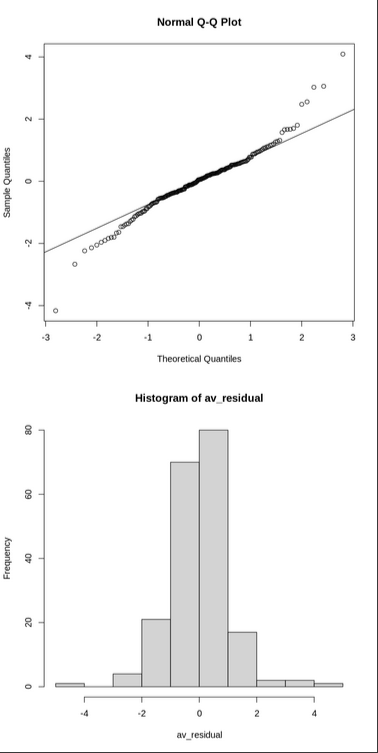
\includegraphics[width=0.5\linewidth]{part01_figures/17.png}
    \caption{Đồ thị phần dư của ảnh hưởng chính giữa Drug và Diff}
    \label{fig:Đồ thị phần dư của ảnh hưởng chính giữa Drug và Diff}
\end{figure}
Với các giả định:
    \begin{itemize}
        \item H0: Phần dư tuân theo phân phối chuẩn.
        \item H1: Phần dư không tuân theo phân phối chuẩn
    \end{itemize}
Nhận xét: với độ tin cậy 5\% thì với giá trị p-value = 2.777e-05 chúng ta đủ cơ sở bác bỏ H0, vậy sai số có phân phối không chuẩn. Nhìn vào biểu đồ, ta thấy rằng ở phần đuôi kéo dài, có một vài điểm bị kéo lệch ra khỏi đường thẳng, Khả năng các điểm nhiễu chính là các điểm ngoại lệ (outliners), tuy nhiên, về mặt tổng quan, dữ liệu vẫn có dạng gần chuẩn.

\newpage
    \begin{lstlisting}
# Kiểm định các nhóm có phương sai đồng nhất hay không
leveneTest(drug_model)
    \end{lstlisting}
Kết quả:
\begin{lstlisting}
A anova: 2 x 3 	
    Df	F value	Pr(>F)
	<int>	<dbl>	<dbl>
group	2	19.06641	2.735522e-08
	195	NA	NA
\end{lstlisting}
Với các giả định:
    \begin{itemize}
        \item H0: Các nhóm có phương sai đồng nhất
        \item H1: Các nhóm không có phương sai đồng nhất
    \end{itemize}
Nhận xét: Với giá trị p-value = 2.735522e-08 < 0.05, ta đủ điều kiện bác bỏ H0, vậy các nhóm có phương sai không đồng nhất.

\begin{lstlisting}
# Kiểm định tính độc lập của phần dư
durbinWatsonTest(drug_model)
plot(drug_model, 1)
\end{lstlisting}

Kết quả:
\begin{lstlisting}
 lag Autocorrelation D-W Statistic p-value
   1       0.2969101      1.398674       0
 Alternative hypothesis: rho != 0
\end{lstlisting}
Với các giả định:
    \begin{itemize}
        \item H0: Không có sự tương quan (độc lập)
        \item H1: Có sự tương quan (không độc lập)
    \end{itemize}
Nhận xét: Với giá trị p-value = 0 nên có sự tương quan dương.
Măc dù với điều kiện phương sai giữa các nhóm không đồng nhất nên sẽ không tiến hành phân
tích ANOVA được, tuy nhiên về mặc trực quan hóa dữ liệu, ta thấy rằng đồ thị phân bố dạng
gần chuẩn, nên ta sẽ tiếp tục đi phân tích các yếu tố ANOVA.

\newpage

\begin{lstlisting}
# Kiểm định độ hiệu quả trung bình giữa các nhóm thuốc
with(processed_islander, pairwise.t.test(Diff, Drug, p.adj = "bonferroni"))
TukeyHSD(aov(Diff~Drug, data=processed_islander), conf.level = 0.95)
plot(TukeyHSD(aov(Diff~Drug, data=processed_islander), conf.level = 0.95))
\end{lstlisting}
Kết quả:
\begin{figure}[H]
    \centering
    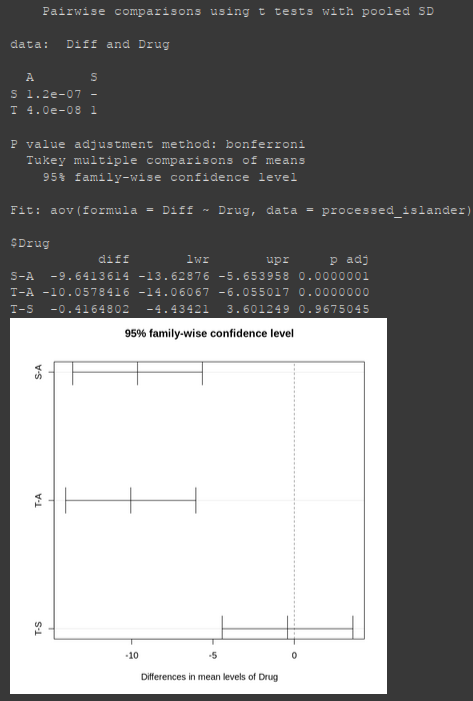
\includegraphics[width=0.7\linewidth]{part01_figures/18.png}
    \caption{Phân tích trung bình giữa các nhóm}
    \label{fig:Phân tích trung bình giữa các nhóm}
\end{figure}
Với các giả thuyết:
    \begin{itemize}
        \item H0: Các giá trị trung bình giữa các cặp bằng nhau
        \item H1: Các giá trị trung bình giữa các cặp không bằng nhau
    \end{itemize}
    Nhìn vào kết quả ta có:
    \begin{itemize}
        \item Nhóm T-S có p-value > 0.05 nên không đủ bác bỏ H0, vậy nhóm này có giá trị trung bình bằng nhau.
        \item Các nhóm còn lại p-value đều có giá trị nhỏ hơn 0.05 (độ tin cậy 95\%) nên ta có cơ sở để bác bỏ H0. Vậy rõ ràng giữa các nhóm nàycó giá trị trung bình là khác nhau. Nghĩa là các nhóm thuốc khác nhau thì cho thấy mức độ ảnh hưởng đến bệnh nhân khác nhau. Nhìn vào kết quả và hình vẽ ta cũng thấy ngay giữa nhóm S-A và T-A có mức độ hiệu quả trung bình khác nhau, T-S có mức độ hiệu quả trung bình như nhau (đồ thị cắt điểm 0)
    \end{itemize}
\end{itemize}
\subsection{Xây dựng và kiểm định mô hình cộng (Additive model)}
\begin{lstlisting}
# Xây dựng mô hình cộng
add_model = lm(Diff~., data=processed_islander)
add_model <- MASS::stepAIC(add_model, k = log(nrow(processed_islander)), trace = 0)
summary(add_model)
\end{lstlisting}
\begin{figure}[H]
    \centering
    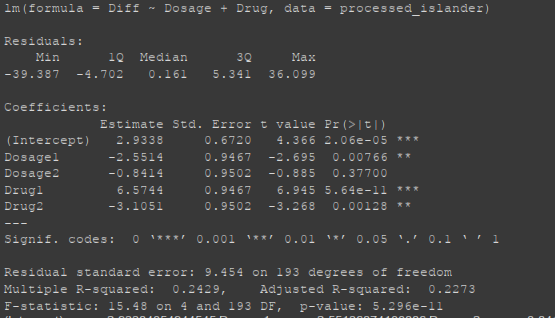
\includegraphics[width=0.8\linewidth]{part01_figures/19.png}
    \caption{Kết quả mô tả của mô hình tuyến tính}
    \label{fig:Kết quả mô tả của mô hình tuyến tính}
\end{figure}

Nhận xét:  Với độ tin cậy 5\%, các biến Dosage và Drug đều có ý nghĩa trong giải thích mô hình. Ta tiến hành kiểm định Shapiro và Breusch-Pagan

\begin{lstlisting}
# Shapiro-Wilk test
av_residual = rstandard(add_model)
shapiro.test(av_residual)

# Trực quan bằng QQ plot
qqnorm(av_residual)
qqline(av_residual)
hist(av_residual)
\end{lstlisting}

Kết quả:
\begin{lstlisting}
    Shapiro-Wilk normality test

data:  av_residual
W = 0.96409, p-value = 6.156e-05
\end{lstlisting}

Với các giả định:
    \begin{itemize}
        \item Phần dư H0: Tuân theo phân phối chuẩn
        \item H1: Phần dư Không tuân theo phân phối chuẩn
    \end{itemize}
Nhận xét: với độ tin cậy 5\% thì với giá trị p-value = 6.156e-05 chúng ta đủ cơ sở bác bỏ H0, vậy sai số có phân phối không chuẩn. Nhìn vào biểu đồ, ta thấy rằng ở phần đuôi kéo dài, có một vài điểm bị kéo lệch ra khỏi đường thẳng --> Khả năng các điểm nhiễu chính là các điểm ngoại lệ (outliners), tuy nhiên, về mặt tổng quan, dữ liệu vẫn có dạng gần chuẩn.

\begin{lstlisting}
# Kiểm định tính độc lập của phần dư
durbinWatsonTest(add_model)
plot(add_model, 1)
\end{lstlisting}

Kết quả:
\begin{lstlisting}
lag Autocorrelation D-W Statistic p-value
   1       0.2550773      1.484015   0.002
Alternative hypothesis: rho != 0
\end{lstlisting}
Với các giả định:
    \begin{itemize}
        \item H0: Không có sự tương quan (độc lập)
        \item H1: Có sự tương quan (không độc lập)
    \end{itemize}
Nhận xét:  Với giá trị p-value = 0.02 < 0.05 nên có sự tương quan dương.

\begin{lstlisting}
# Kiểm định  Breusch-Pagan
bptest(add_model)
\end{lstlisting}
Kết quả:
\begin{lstlisting}
	studentized Breusch-Pagan test

data:  add_model
BP = 9.0739, df = 4, p-value = 0.05928
\end{lstlisting}
Với các giả định:
    \begin{itemize}
        \item H0: phương sai không đổi
        \item H1: phương sai thay đổi
    \end{itemize}
Nhận xét:  Với p-value=0.059 > 0.05 thì ta không đủ điều kiện bác bỏ H0. Vậy phương sai của mô hình không thay đổi.

Như vậy, mô hình cộng được xây dựng như sau:
\[
\text{Diff} = 2.9338 - 2.5514 \times \text{Dosage}_1 - 0.8414 \times \text{Dosage}_2 + 6.5744 \times \text{Drug}_1 - 3.1051 \times \text{Drug}_2
\]
 Với Adjusted R-squared = 0.2273, các biến giải thích được 22,73\% ý nghĩa của mô hình, điều này có nghĩa rằng việc phục hồi trí nhớ sẽ bị chi phối bởi rất nhiều yếu tố (phần lớn là bản thân của ngươi bệnh trầm cảm), chứ không chỉ mỗi tác động của thuốc. Sau đây sẽ là một số nhận xét của mô hình này:
 \begin{itemize}
     \item Hiệu ứng của liều lượng thứ nhất so với mức cơ bản. Giảm thời gian hoàn thành bài kiểm tra trí nhớ xuống 2.5514 giây, có ý nghĩa thống kê (p < 0.01).
     \item Dosage2: Hiệu ứng của liều lượng thứ hai so với mức cơ bản. Giảm thời gian hoàn thành bài kiểm tra trí nhớ xuống 0.8414 giây, nhưng không có ý nghĩa thống kê (p = 0.377).
     \item Drug1: Hiệu ứng của loại thuốc thứ nhất so với mức cơ bản. Tăng thời gian hoàn thành bài kiểm tra trí nhớ lên 6.5744 giây, có ý nghĩa thống kê cao (p < 0.001).
    \item Drug2: Hiệu ứng của loại thuốc thứ hai so với mức cơ bản. Giảm thời gian hoàn thành bài kiểm tra trí nhớ xuống 3.1051 giây, có ý nghĩa thống kê (p < 0.01).
    \item  F-statistic: 15.48 với p-value = 5.296e-11, cho thấy mô hình tổng thể có ý nghĩa thống kê.
 \end{itemize}
 Kết luận: Nếu xem bản thân loại thuốc và liều thuốc tương tác một cách độc lập, thì sau đây là khuyến nghị cho bác sỹ:
 \begin{itemize}
     \item Liều lượng: Liều lượng thứ nhất có ảnh hưởng đáng kể đến thời gian hoàn thành bài kiểm tra trí nhớ, trong khi liều lượng thứ hai không có ảnh hưởng đáng kể. Khuyến nghị bác sỹ dùng liều lượng thứ nhất (liều lượng thấp). 
     \item Loại thuốc: Cả hai loại thuốc đều có ảnh hưởng đáng kể đến thời gian hoàn thành bài kiểm tra trí nhớ, với loại thuốc thứ nhất tăng thời gian và loại thuốc thứ hai giảm thời gian. Khuyến nghị bác sỹ sử cho bệnh nhân sử dụng loại thuốc thứ hai (loại thuốc S)
 \end{itemize}
 Thực tế thì 2 nhân tố này ảnh hưởng trực tiếp đến nhau và cho kết quả khác với mô hình cộng (phân tích ảnh hưởng đơn ở phần trước) vì vậy, cần phải cẩn thận cân nhắc khi sử dụng thuốc tránh đem lại hậu quả không mong muốn ngoài tầm kiểm soát.

 \subsection{Cải tiến mô hình}
 Như chúng ta đã thấy ở các bước phân tích trên, khi phân tích ảnh hưởng chính cũng như xây dựng mô hình tuyến tính, có một số yêu cầu chưa thoả mãn (ví dụ như tính chuẩn, tính độc lập của phương sai), vì vậy, trong phần này chúng ta sẽ tập trung sử lý dữ liệu cho phù hợp hơn. Như đã nhận định ở trên, hiện tại dữ liệu chúng ta đang tồn tại các điểm ngoại lai và cực ngoại lai, trong thí nghiệm này, chúng ta tiến hành loại bỏ các điểm này và tiến hành khảo sát. Ở phần này, tôi sẽ không trình bày chi tiết từng bước như trước (vì các bước thực hiện như nhau, mã thực thi đính kèm); chỉ trình bày những điểm thay đổi chính so với việc phân tích từ tập dữ liệu thô ban đầu.

 Đầu tiên ta sẽ tiến hành khảo sát các điểm ngoại lai bằng lệnh sau

 \begin{lstlisting}
 # Khảo sát ngoại lai theo biến diff
diff_data = processed_islander["Diff"]
outliers_index = list()
extreme_outliers_index = list()

for (i in 1:ncol(diff_data)) {
  # Tính toán Q1, Q3 và IQR
  Q1 = quantile(diff_data[, i], 0.25, na.rm = TRUE)
  Q3 = quantile(diff_data[, i], 0.75, na.rm = TRUE)
  IQR = Q3 - Q1

  # Xác định ngoại lai
  outliers_index_i = diff_data[, i] < (Q1 - 1.5 * IQR) | diff_data[, i] > (Q3 + 1.5 * IQR)
  # outliers_i = diff_data[diff_data[, i] < (Q1 - 1.5 * IQR) | diff_data[, i] > (Q3 + 1.5 * IQR), i]

  # Lưu trữ ngoại lai
  field_name = names(diff_data)[i]
  outliers_index[[field_name]] = which(outliers_index_i)

  # Xác định cực ngoại lai
  extreme_outliers_index_i = diff_data[, i] < (Q1 - 3 * IQR) | diff_data[, i] > (Q3 + 3 * IQR)
  extreme_outliers_index[[field_name]] = which(extreme_outliers_index_i)
}
# In kết quả theo từng biến ra màn hình
for (i in 1:ncol(diff_data)) {
  print(paste("Biến:", names(diff_data)[i]))
  print(paste("Số ngoại lai:", length(outliers_index[[names(diff_data)[i]]])))
  print(paste("Số cực ngoại lai:", length(extreme_outliers_index[[names(diff_data)[i]]])))
}

# Tìm tổng số quan trắc ngoại lai và cực ngoại lai thực sự
outliers = c()
extreme_outliners = c()
for (i in 1:ncol(diff_data)){
    outliers = c(outliers, outliers_index[[names(diff_data)[i]]])
    extreme_outliners = c(extreme_outliners, extreme_outliers_index[[names(diff_data)[i]]])
}

outliers = unique(outliers)
extreme_outliners = unique(extreme_outliners)
print(paste("Tổng số ngoại lai:", length(outliers)))
print(paste("Tổng số cực ngoại lai:", length(extreme_outliners)))
 \end{lstlisting}

\newpage
 Kết quả:
 \begin{lstlisting}
[1] "Biến: Diff"
[1] "Số ngoại lai: 20"
[1] "Số cực ngoại lai: 5"
[1] "Tổng số ngoại lai: 20"
[1] "Tổng số cực ngoại lai: 5"
 \end{lstlisting}

 Như vậy, tổng số ngoại lai và cực ngoại là là 25 samples (chiếm khoảng 12\%). Ta tiến hành loại bỏ các điểm này

 \begin{lstlisting}
# Loại bỏ các điểm ngoại lai và cực ngoại lai
rm_outliner_islander = processed_islander[-extreme_outliners,]
rm_outliner_islander = rm_outliner_islander[-outliers,]

# Kiểm tra lại số lượng dữ liệu
dim(rm_outliner_islander)
str(rm_outliner_islander)
 \end{lstlisting}
Kết quả
\begin{lstlisting}
173 3
'data.frame':	173 obs. of  3 variables:
 $ Dosage: Factor w/ 3 levels "1","2","3": 1 1 1 1 1 1 1 1 1 1 ...
 $ Drug  : Factor w/ 3 levels "A","S","T": 1 1 1 1 1 1 1 1 1 1 ...
 $ Diff  : num  -2.3 -0.9 -4.6 -0.5 0.1 -8.3 11.9 -1.5 -11.2 12 ...
\end{lstlisting}

\newpage
Như vậy, sau khi loại bỏ các điểm ngoại lai ta thu còn lại 173 samples. Ta tiến hành trực quan hoá đồ thị của dữ liệu

\begin{lstlisting}
# Biến phụ thuộc Diff
ggplot(rm_outliner_islander, aes(x = Diff)) +
  geom_histogram(aes(y = ..density..), bins = 30, color = "black", fill = "lightblue") +
  geom_density(alpha = 0.2, fill = "#FF6666") +
  stat_function(fun = dnorm, args = list(mean = mean(rm_outliner_islander$Diff, na.rm = TRUE), sd = sd(rm_outliner_islander$Diff, na.rm = TRUE)),
                color = "blue", size = 1) +
  theme_minimal() +
  labs(title = "Histogram of Diff variable", x = "Diff", y = "Density")
  summary(rm_outliner_islander$Diff)
\end{lstlisting}

Kết quả:
\begin{figure}[H]
    \centering
    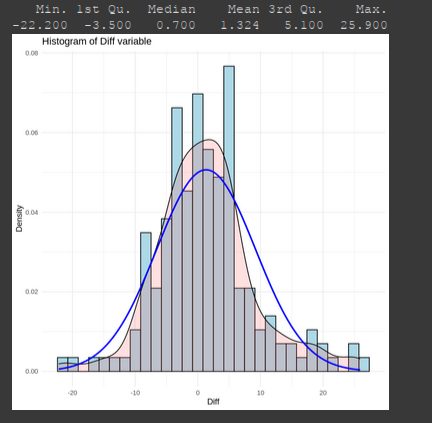
\includegraphics[width=0.7\linewidth]{part01_figures/20.png}
    \caption{Trực quan hóa dữ liệu của biến Diff}
    \label{fig:Trực quan hóa dữ liệu của biến Diff}
\end{figure}

Nhận xét: Sau khi loại bỏ các điểm ngoại lai và cực ngoại lai, ta thu được đồ thị gần chuẩn và có hình dáng tốt hơn trước khi loại.


Tiếp theo chúng ta sẽ tiến hành xây dựng mô hình tương tác và kiểm định các giả thuyết

\begin{lstlisting}
int_model = aov(Diff~ Dosage * Drug, rm_outliner_islander)
\end{lstlisting}

\begin{lstlisting}
# Kiểm định shaoiro test
av_residual = rstandard(int_model)
shapiro.test(av_residual)

# Trực quan bằng QQ plot
qqnorm(av_residual)
qqline(av_residual)
hist(av_residual)
\end{lstlisting}

Kết quả:

\begin{lstlisting}
             Df Sum Sq Mean Sq F value   Pr(>F)    
Dosage        2    190    94.8   2.115    0.124    
Drug          2    957   478.4  10.670 4.40e-05 ***
Dosage:Drug   4   2166   541.6  12.079 1.25e-08 ***
Residuals   164   7354    44.8                     
---
Signif. codes:  0 '***' 0.001 '**' 0.01 '*' 0.05 '.' 0.1 ' ' 1

	Shapiro-Wilk normality test

data:  av_residual
W = 0.98596, p-value = 0.08056
\end{lstlisting}
\begin{figure}[H]
    \centering
    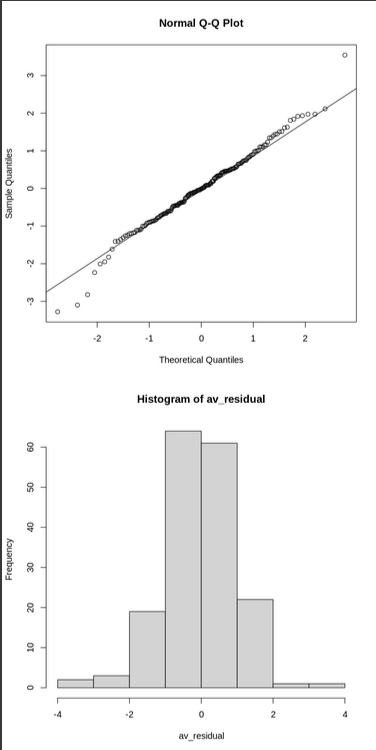
\includegraphics[width=0.7\linewidth]{part01_figures/21.png}
    \caption{Phân phối của phần dư sau khi cải tiến}
    \label{fig:Phân phối của phần dư sau khi cải tiến}
\end{figure}
Với giả định \begin{itemize}
    \item H0: Phần dư tuân theo phân phối chuẩn
    \item H1: Phần dư không tuân theo phân phối chuẩn
\end{itemize}

Với giả độ tin cậy 0.05 thì ta không đủ điều kiện bác bỏ H0, vậy phần dư tuân theo phân phối chuẩn. Măc khác ta thấy rằng thấy bản thân liều lượng (Dosage) sẽ không tác động đến hiệu quả của người sử dụng thuốc, tuy nhiên chúng có mối liên hệ mật thiết (có tương tác) với loại thuốc.
\newpage
Tiếp theo chúng ta đi kiểm định tính độc lập của phần dư:
\begin{lstlisting}
# Kiểm định tính độc lập của phần dư
durbinWatsonTest(int_model)
plot(int_model, 1)
\end{lstlisting}
Kết quả
\begin{lstlisting}
 lag Autocorrelation D-W Statistic p-value
   1      -0.1264805      2.251922   0.304
 Alternative hypothesis: rho != 0
\end{lstlisting}
\begin{figure}[H]
    \centering
    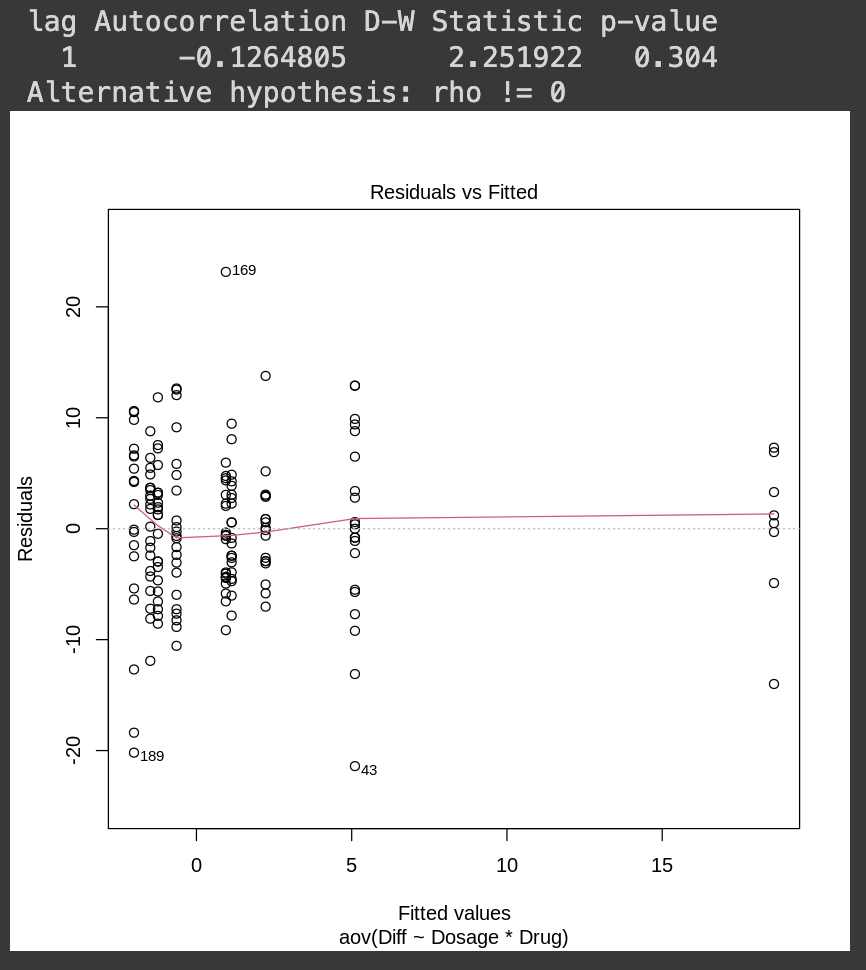
\includegraphics[width=0.8\linewidth]{part01_figures/23.png}
    \caption{Đồ thị  Residuals}
    \label{fig:Đồ thị  Residuals}
\end{figure}
Với mức ý nghĩa 5\%, ta thấy rằng mô hình có phần dư độc lập.
Tiếp tục Kiểm định các nhóm có phương sai đồng nhất hay không

\begin{lstlisting}
# Kiểm định các nhóm có phương sai đồng nhất hay không
leveneTest(int_model)
\end{lstlisting}

Kết quả
\begin{lstlisting}
A anova: 2 x 3
Df	F value	Pr(>F)
<int>	<dbl>	<dbl>
group	8	1.440304	0.1833148
164	NA	NA

\end{lstlisting}

Với mức ý nghĩa 5\%, ta thấy mô hình có phương sai của các nhóm đồng nhất. Như vậy, ta đủ điều kiện để phân tích ANOVA. Bước tiếp theo, chúng ta sẽ tiến hành kiểm tra tương tác đơn và tương tác chính như phần trước.

\begin{itemize}
    \item \textbf{Bước 1: Kiểm tra sự tương tác }
    \begin{lstlisting}
summary(int_model)
plot(interactionMeans(int_model))
    \end{lstlisting}

Kết quả:
\begin{figure}[H]
    \centering
    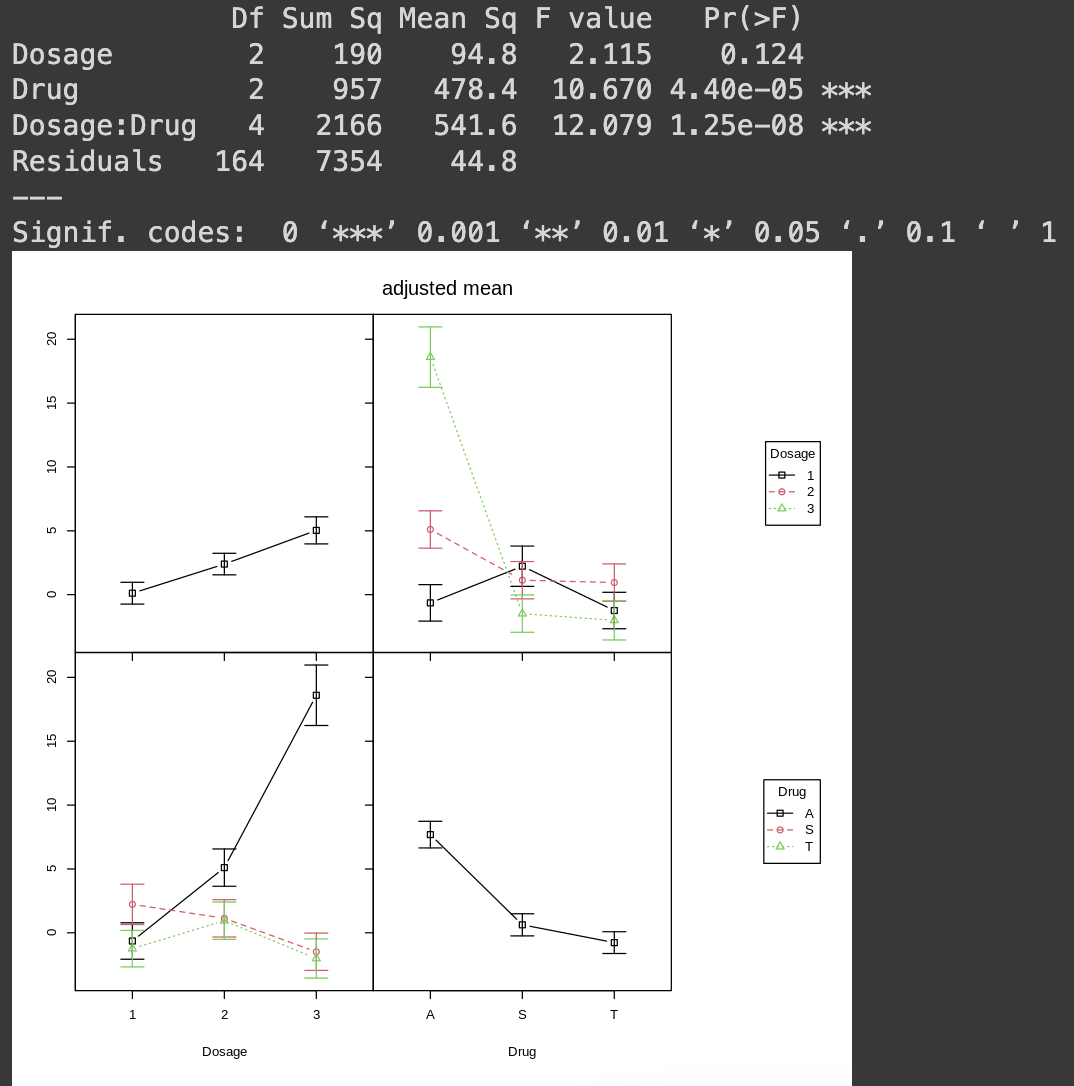
\includegraphics[width=0.7\linewidth]{part01_figures/24.png}
    \caption{Tương tác giữa Drug và Dosage}
    \label{fig:Tương tác giữa Drug và Dosage}
\end{figure}
Nhận xét: Với mức ý nghĩa 5\%, ta thấy giữa `Dosage` và `Drug` có sự tương tác với nhau (p-value=1.25e-08). Sự kết hợp giữa hàm lượng thuốc và loại thuốc có ảnh hưởng rất lớn đến thời gian hoàn thành bài kiểm tra, cho thấy rằng không chỉ từng yếu tố riêng lẻ mà sự kết hợp giữa chúng cũng rất quan trọng. Về phần nhận xét chi tiết xem lại phần đầu tiên vì kết quả biểu đồ giống với phân tích của phần đầu.

    \item \textbf{Bước 2: Phân tích ảnh hưởng đơn}
    \begin{itemize}
        \item[a.] \textbf{Phân tích ảnh hưởng đơn của liều lượng ở mỗi loại thuốc}
        \begin{lstlisting}
testInteractions(int_model, fixed = "Drug", across = "Dosage")
        \end{lstlisting}
    Kết quả:
    \begin{figure}[H]
        \centering
        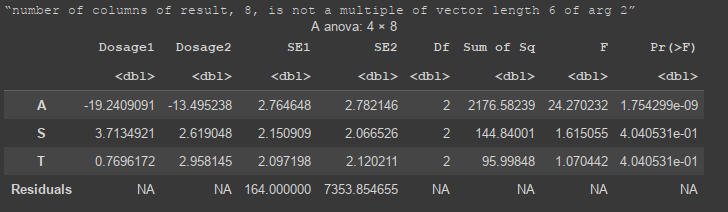
\includegraphics[width=0.8\linewidth]{part01_figures/25.png}
        \caption{Kết quả ảnh hưởng đơn của liều lượng ở mỗi loại thuốc}
        \label{fig:Kết quả ảnh hưởng đơn của liều lượng ở mỗi loại thuốc}
    \end{figure}
    Giả định:
        \begin{itemize}
            \item H0: Liều lượng Không ảnh hưởng đến hiệu quả thuốc
            \item H1: Liều lượng Có ảnh hưởng đến hiệu quả của thuốc
        \end{itemize}
    Nhận xét: Với kết quả phân tích ta có một số nhận xét như sau, với độ tin cậy 5\% thì:
        \begin{itemize}
            \item Liều lượng có ảnh hưởng đến kết quả của loại thuốc A
            \item Liều lượng không ảnh hưởng đến kết quả của lọai thuốc S và T
        \end{itemize}
    \item [b].\textbf{ Phân tích ảnh hưởng đơn của thuốc ở mỗi liều lượng}
        \begin{lstlisting}
testInteractions(int_model, fixed = "Dosage", across = "Drug")
        \end{lstlisting}
        \newpage
        Kết quả:
        \begin{figure}[H]
            \centering
            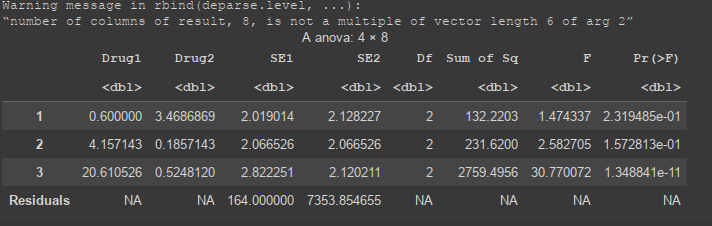
\includegraphics[width=0.8\linewidth]{part01_figures/26.png}
            \caption{Kết quả ảnh hưởng đơn của thuốc ở mỗi liều lượng}
            \label{fig:Kết quả ảnh hưởng đơn của thuốc ở mỗi liều lượng}
        \end{figure}
        Với giả định
        \begin{itemize}
            \item H0: Các loại thuốc sẽ không tác động ở mỗi liều lượng
            \item H1: Các loại thuốc sẽ có tác động ở mỗi liều lượng
        \end{itemize}
        Nhận xét: Với kết quả phân tích ta có một số nhận xét như sau, với độ tin cậy 5\% thì: Hầu hết các loại thuốc sẽ có tác động ở liều lượng cao; liều lượng thấp và trung bình cho kết quả không đáng kể.
         \item [c.] \textbf{Phân tích ảnh hưởng đơn giữa các nhóm thuốc ứng với mỗi liều lượng}
        \begin{lstlisting}
options(contrasts = c(unordered="contr.sum", ordered="contr.poly"))
A_vs_S = list(Drug = c(1, -1, 0))
A_vs_T = list(Drug = c(1, 0, -1))
S_vs_T = list(Drug = c(0, 1, -1))
# Nhóm A và S
testInteractions(int_model, custom = c(A_vs_S), fixed = "Dosage", adjustment = "bonferroni")
        \end{lstlisting}
    \begin{figure}[H]
            \centering
            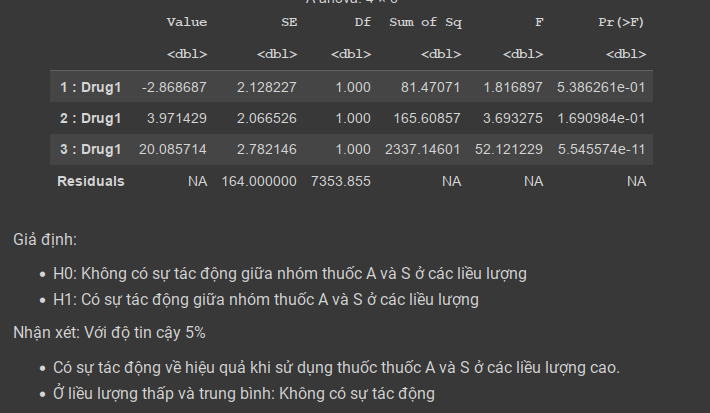
\includegraphics[width=0.7\linewidth]{part01_figures/27.png}
            \caption{Ảnh hưởng giữa nhóm A và S}
            \label{fig:Ảnh hưởng giữa nhóm A và S}
        \end{figure}
                
        Với các giả định:
        \begin{itemize}
            \item H0: Không có sự tác động giữa nhóm thuốc A và S ở các liều lượng
            \item H1: Có sự tác động giữa nhóm thuốc A và S ở các liều lượng
        \end{itemize}
        Nhận xét: Với độ tin cậy 5\% Có sự tác động về hiệu quả khi sử dụng thuốc thuốc A và S ở các liều lượng cao.Ở liều lượng thấp và trung bình: Không có sự tác động.

    \begin{lstlisting}
# Nhóm A và T
testInteractions(int_model, custom = c(A_vs_T), fixed = "Dosage", adjustment = "bonferroni")
    \end{lstlisting}
    \begin{figure}[H]
        \centering
        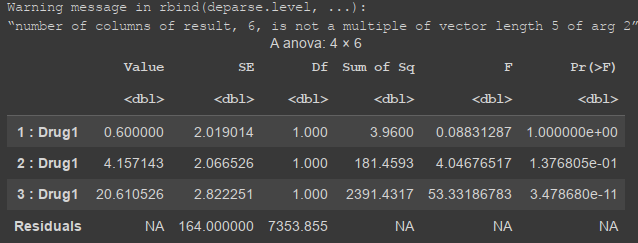
\includegraphics[width=0.7\linewidth]{part01_figures/28.png}
        \caption{Ảnh hưởng giữa nhóm A và T}
        \label{fig:Ảnh hưởng giữa nhóm A và T}
    \end{figure}
    
    Với các giả định:
        \begin{itemize}
            \item H0: Không có sự tác động giữa nhóm thuốc A và T ở các liều lượng
            \item H1: Có sự tác động giữa nhóm thuốc A và T ở các liều lượng
        \end{itemize}
        Nhận xét: Với độ tin cậy 5\% Có sự tác động về hiệu quả khi sử dụng thuốc thuốc A và T ở các liều lượng cao.Ở liều lượng thấp và trung bình: Không có sự tác động.

    \begin{lstlisting}
# Nhóm S và T
testInteractions(int_model, custom = c(S_vs_T), fixed = "Dosage", adjustment = "bonferroni")
    \end{lstlisting}
    <chèn ảnh>
    \begin{figure}[H]
            \centering
            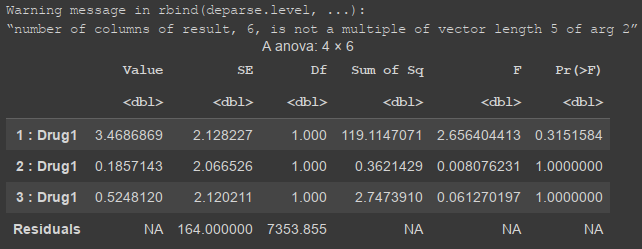
\includegraphics[width=0.8\linewidth]{part01_figures/29.png}
            \caption{Ảnh hưởng giữa S và T}
            \label{fig:Ảnh hưởng giữa S và T}
        \end{figure}
                Với các giả định:
        \begin{itemize}
            \item H0: Không có sự tác động giữa nhóm thuốc S và T ở các liều lượng
            \item H1: Có sự tác động giữa nhóm thuốc S và T ở các liều lượng
        \end{itemize}
        Nhận xét: Với độ tin cậy 5\% thì không có sự khác biệt nào ở cả 3 liều lượng.
    \item [d.] \textbf{Phân tích ảnh hưởng đơn giữa các nhóm liều lượng ứng với mỗi loại thuốc}
        \begin{lstlisting}
ptions(contrasts = c(unordered="contr.sum", ordered="contr.poly"))
low_vs_medium = list(Dosage = c(1, -1, 0))
low_vs_high = list(Dosage = c(1, 0, -1))
medium_vs_high = list(Dosage = c(0, 1, -1))
        \end{lstlisting}

        \begin{lstlisting}
# Nhóm thấp và trung bình
testInteractions(int_model, custom = c(low_vs_medium), fixed = "Drug", adjustment = "bonferroni")
        \end{lstlisting}
        Kết quả:
        \begin{figure}[H]
            \centering
            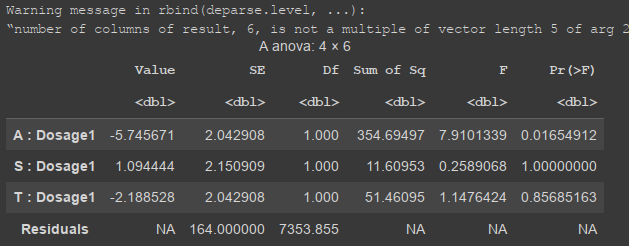
\includegraphics[width=0.8\linewidth]{part01_figures/30.png}
            \caption{Ảnh hưởng giữa nhóm thấp và trung bình}
            \label{fig:Ảnh hưởng giữa nhóm thấp và trung bình}
        \end{figure}

        Với các giả định:
        \begin{itemize}
            \item H0: Không có sự tương tác nhau giữa liều thấp và liều trung bình
            \item H1: Có sự tương tác nhau giữa liều thấp và liều trung bình
        \end{itemize}
        Nhận xét: Với độ tin cậy 5\% Ở loại thuốc A: Có sự tương tác về hiệu quả khi sử dụng thuốc ở các liều lượng thấp và liều lượng trung bình; Ở loại thuốc S và T: Không có sự tương tác có ý nghĩa thống kê.
    \begin{lstlisting}
# Nhóm thấp và cao
testInteractions(int_model, custom = c(low_vs_high), fixed = "Drug", adjustment = "none")
    \end{lstlisting}
    Kết quả:
    \begin{figure}[H]
        \centering
        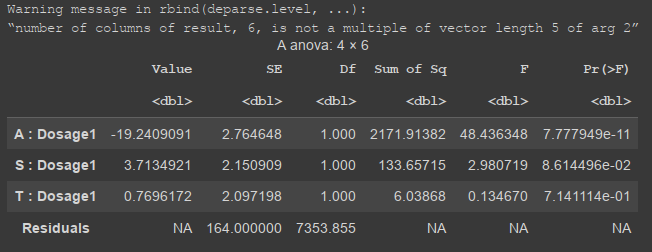
\includegraphics[width=0.8\linewidth]{part01_figures/31.png}
        \caption{Ảnh hưởng giữa nhóm thấp và cao}
        \label{fig:Ảnh hưởng giữa nhóm thấp và cao}
    \end{figure}
    Với các giả định:
        \begin{itemize}
            \item H0: Không có tương tác nhau giữa liều thấp và liều cao
            \item H1: Có tương tác nhau giữa liều thấp và liều cao
        \end{itemize}
    Nhận xét: Với độ tin cậy 5\% Ở loại thuốc A: Có sự tương tác về hiệu quả khi sử dụng thuốc ở các liều lượng thấp và liều lượng cao; Ở loại thuốc S và T: Không có sự tương tác có ý nghĩa thống kê.
    \begin{lstlisting}
# Nhóm trung bình và cao
testInteractions(int_model, custom = c(medium_vs_high), fixed = "Drug", adjustment = "none")
    \end{lstlisting}
    Kết quả:
    \begin{figure}[H]
        \centering
        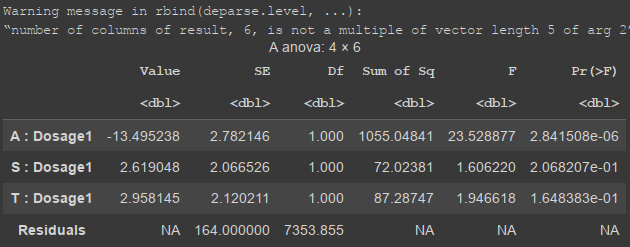
\includegraphics[width=0.8\linewidth]{part01_figures/32.png}
        \caption{Tương tác giữa nhóm trung bình vào cao}
        \label{fig:Tương tác giữa nhóm trung bình vào cao}
    \end{figure}
    
    Với các giả định:
        \begin{itemize}
            \item H0: Không có sự tương tác giữa liều trung bình và liều cao
            \item Có sự tương tác giữa liều trung bình và liều cao
        \end{itemize}
    Nhận xét: Với độ tin cậy 5\% Ở loại thuốc A: Có sự tương tác về hiệu quả khi sử dụng thuốc ở các liều lượng trung bình và liều lượng cao; Ở loại thuốc S và T: Không có sự tương tác có ý nghĩa thống kê.
    
    \item \textbf{Kết luận}: \textbf{Kết quả này giống với kết quả phân tích trước đó. Tuy nhiên các tính chất kiểm định về chuẩn cho đánh giá ANOVA đã cho kết quả tốt hơn so với trước khi chưa xử lý dữ liệu.}
    \end{itemize}
   \item \textbf{Bước 3. Phân tích ảnh hưởng chính}
   \begin{itemize}
       \item \textbf{Phân tích ảnh hưởng chính của Dosage với hiệu quả của bài kiểm tra trí nhớ}
       \begin{lstlisting}
dosage_model = aov(Diff~Dosage, data = rm_outliner_islander)
summary(dosage_model)
       \end{lstlisting}
       Kết quả:
       \begin{lstlisting}
             Df Sum Sq Mean Sq F value Pr(>F)
Dosage        2    190   94.84   1.539  0.218
Residuals   170  10477   61.63               
       \end{lstlisting}
    Nhận xét: Với mức ý nghĩa 0.05, ta thấy rằng Dosage không có ý nghĩa trong việc giải thích mô hình. Theo nguyên tắc thì ta không cần phải đi kiểm định các giả thuyết cho biến này. Tuy nhiên chúng ta vẫn kiểm định để xem kết quả cải thiện như thế nào so với trước đó.
    \begin{lstlisting}
# Shapiro-Wilk test
av_residual = rstandard(dosage_model)
shapiro.test(av_residual)

# Trực quan bằng QQ plot
qqnorm(av_residual)
qqline(av_residual)
hist(av_residual)
    \end{lstlisting}
    Kết quả:
    \begin{lstlisting}
	Shapiro-Wilk normality test
data:  av_residual
W = 0.96742, p-value = 0.0004441
    \end{lstlisting}

    \begin{figure}[H]
        \centering
        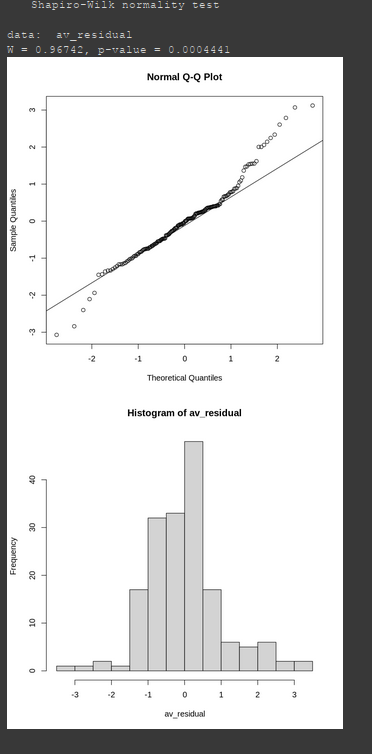
\includegraphics[width=0.6\linewidth]{part01_figures/33.png}
        \caption{Shapiro-test}
        \label{fig:Shapiro-test}
    \end{figure}

    Nhận xét: Giá trị p-value đã tăng lên rất nhiều (mặc dù < 0.05), hình dáng đồ thị gần chuẩn hơn so với trước khi chưa xử lý dữ liệu.
   \end{itemize}
    \begin{lstlisting}
# Kiểm định các nhóm có phương sai đồng nhất hay không
leveneTest(dosage_model)
    \end{lstlisting}
    Kết quả:
    \begin{lstlisting}
A anova: 
2 x 3 	Df	F value	Pr(>F)
	<int>	<dbl>	<dbl>
group	2	4.442547	0.01316301
	170	NA	NA
    \end{lstlisting}
    Nhận xét:
    Với các giả định:
        \begin{itemize}
            \item Các nhóm có phương sai đồng nhất
            \item Các nhóm không có phương sai đồng nhất
        \end{itemize}
    Nhận xét:Với giá trị p-value = 0.013 > 0.05, ta không điều kiện bác bỏ H0, vậy các nhóm có phương sai đồng nhất (trước đó là không đồng nhất) trước đó điều kiện  này không thỏa mãn.
    \begin{lstlisting}
# Kiểm định tính độc lập của phần dư
durbinWatsonTest(dosage_model)
plot(dosage_model, 1)
    \end{lstlisting}
    Kết quả:
    \begin{figure}[H]
        \centering
        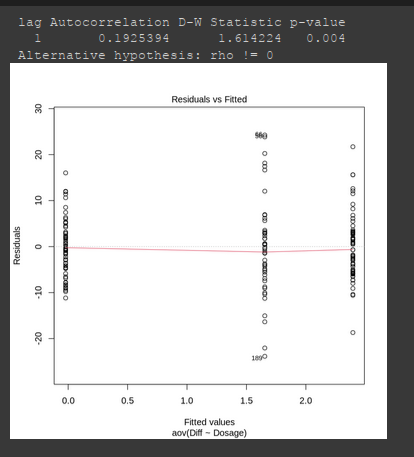
\includegraphics[width=0.8\linewidth]{part01_figures/34.png}
        \caption{Kiểm định độc lập phần dư}
        \label{fig:Kiểm định độc lập phần dư_}
    \end{figure}
        Nhận xét:
    Với các giả định:
        \begin{itemize}
            \item H0: Không có sự tương quan (độc lập)
            \item H1: Có sự tương quan (không độc lập)
        \end{itemize}
    Nhận xét:Với giá trị p-value = 0.02 nên có sự tương quan dương, tuy nhiên kết quả này lớn hơn kết quả trước đó (=0).
    \begin{lstlisting}
# Kiểm định trung bình giữa các nhóm liều lượng
with(rm_outliner_islander, pairwise.t.test(Diff, Dosage, p.adj = "bonferroni"))
TukeyHSD(aov(Diff~Dosage, data=rm_outliner_islander), conf.level = 0.95)
plot(TukeyHSD(aov(Diff~Dosage, data=rm_outliner_islander), conf.level = 0.95))
    \end{lstlisting}
    Kết quả:
    \begin{figure}[H]
        \centering
        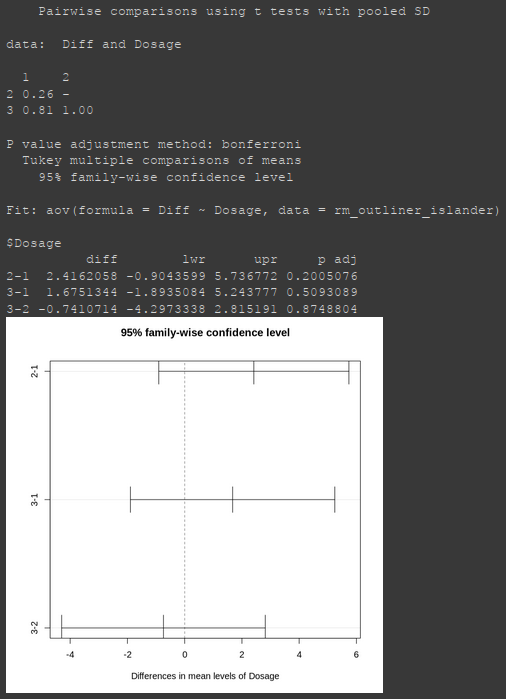
\includegraphics[width=0.8\linewidth]{part01_figures/35.png}
        \caption{Kiểm định trung bình}
        \label{fig:Kiểm định trung bình_}
    \end{figure}

    Với các giả định:
        \begin{itemize}
            \item H0: Các giá trị trung bình giữa các cặp bằng nhau
            \item H1: Các giá trị trung bình giữa các cặp không bằng nhau
        \end{itemize}
    Nhận xét:Các cặp có p-value đều có giá trị lớn hơn 0.05 (độ tin cậy 95\%) nên ta cơ sở để bác bỏ H0. Vậy rõ ràng giữa các nhóm này có giá trị trung bình là như nhau.Để rõ hơn, ta tiến hành kiểm định Tukey's. Nhìn vào kết quả và hình vẽ ta cũng thấy ngay mức độ hiệu quả trung bình như nhau ở 3 nhóm(đồ thị cắt điểm 0). \textbf{Kết quả trước đó cho ta thấy rằng  3-2 và 1-2 có mức độ hiệu quả trung bình như nhau  và 3-1 là khác nhau.}

    \begin{lstlisting}
# ttest
A_vs_S = list(Dosage = c(1, -1, 0))
A_vs_T = list(Dosage = c(1, 0, -1))
S_vs_T = list(Dosage = c(0, 1, -1))
testInteractions(dosage_model, custom = A_vs_S, adjustment = 'bonferroni')
print("----------------------------------------------------------")
testInteractions(dosage_model, custom = A_vs_T, adjustment = 'bonferroni')
print("----------------------------------------------------------")
testInteractions(dosage_model, custom = S_vs_T, adjustment = 'bonferroni')
    \end{lstlisting}
\begin{figure}[H]
    \centering
    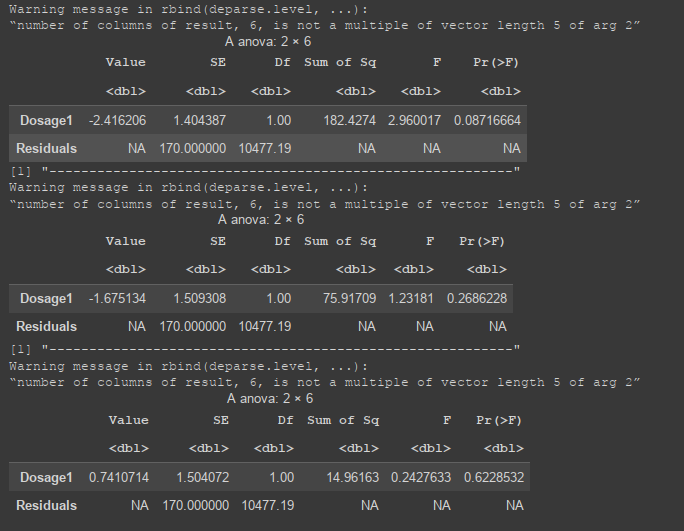
\includegraphics[width=0.8\linewidth]{part01_figures/36.png}
    \caption{Kết quả t-test}
    \label{fig:Kết quả t-test}
\end{figure}
    
    Với các giả định:
    \begin{itemize}
        \item H0: Không có sự tương tác giữa 2 nhóm thuốc được nhắc đến
        \item H1: Có sự tương tác giữa 2 nhóm thuốc được nhắc đến
    \end{itemize}
    Nhận xét: Với p-value=0.05, ta có kết luận như sau: cả 3 nhóm đều có sự tương tác mang ý nghĩa thống kê (giống kết quả trước đó).

    \item \textbf{Phân tích ảnh hưởng chính của Drug với hiệu quả của bài kiểm tra trí nhớ}
    \begin{lstlisting}
drug_model = aov(Diff~Drug, data = rm_outliner_islander)
summary(drug_model)
    \end{lstlisting}
    Kết quả:
    \begin{lstlisting}
             Df Sum Sq Mean Sq F value   Pr(>F)    
Drug          2    896   447.8   7.791 0.000579 ***
Residuals   170   9771    57.5                     
---
Signif. codes:  0 '***' 0.001 '**' 0.01 '*' 0.05 '.' 0.1 ' ' 1
    \end{lstlisting}
    Nhận xét: Với mức ý nghĩa 0.05, ta thấy rằng Drug có ý nghĩa trong việc giải thích mô hình.
    \begin{lstlisting}
# Shapiro-Wilk test
av_residual = rstandard(drug_model)
shapiro.test(av_residual)

# Trực quan bằng QQ plot
qqnorm(av_residual)
qqline(av_residual)
hist(av_residual)
    \end{lstlisting}

    Kết quả:
    \begin{lstlisting}
	Shapiro-Wilk normality test

data:  av_residual
W = 0.9859, p-value = 0.07921
    \end{lstlisting}

    \begin{figure}
        \centering
        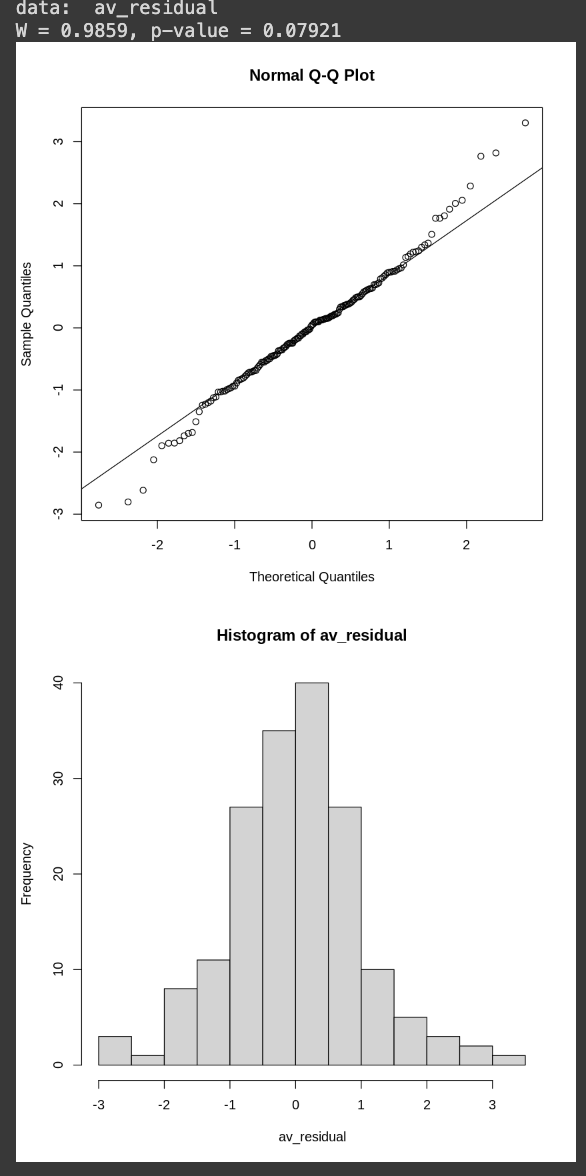
\includegraphics[width=0.5\linewidth]{part01_figures/38.png}
        \caption{Shapiro-Wilk test và đồ thị phần dư}
        \label{fig:Shapiro-Wilk test và đồ thị phần dư}
    \end{figure}

    Với các giả định:
    \begin{itemize}
        \item H0: Tuân theo phân phối chuẩn
        \item H1: Không tuân theo phân phối chuẩn
    \end{itemize}
    Nhận xét: với độ tin cậy 5\% thì với giá trị p-value =0.07921 chúng ta không đủ cơ sở bác bỏ H0, vậy sai số có phân phối chuẩn. Nhìn vào biểu đồ, ta thấy rằng ở phần đuôi kéo dài, có một vài điểm bị kéo lệch ra khỏi đường thẳng về mặt tổng quan, dữ liệu vẫn có dạng gần chuẩn (trước đó là không chuẩn)

    \begin{lstlisting}
# Kiểm định các nhóm có phương sai đồng nhất hay không
leveneTest(drug_model)
    \end{lstlisting}
    Kết quả:
    \begin{lstlisting}
A anova: 
2 x 3 	Df	F value	Pr(>F)
	<int>	<dbl>	<dbl>
group	2	11.12926	2.87001e-05
	170	NA	NA
    \end{lstlisting}
    Với các giả định:
    \begin{itemize}
        \item H0: Các nhóm có phương sai đồng nhất
        \item H1: Các nhóm không có phương sai đồng nhất
    \end{itemize}
    Nhận xét: Nhận xét: Với giá trị p-value = 2.87001e-05 < 0.05, ta đủ điều kiện bác bỏ H0, vậy các nhóm có phương sai không đồng nhất, tuy nhiên kết quả có giá trị p-value cao hơn trước (2.735522e-08).
\begin{lstlisting}
# Kiểm định tính độc lập của phần dư
durbinWatsonTest(drug_model)
plot(drug_model, 1)
\end{lstlisting}
\begin{figure}
    \centering
    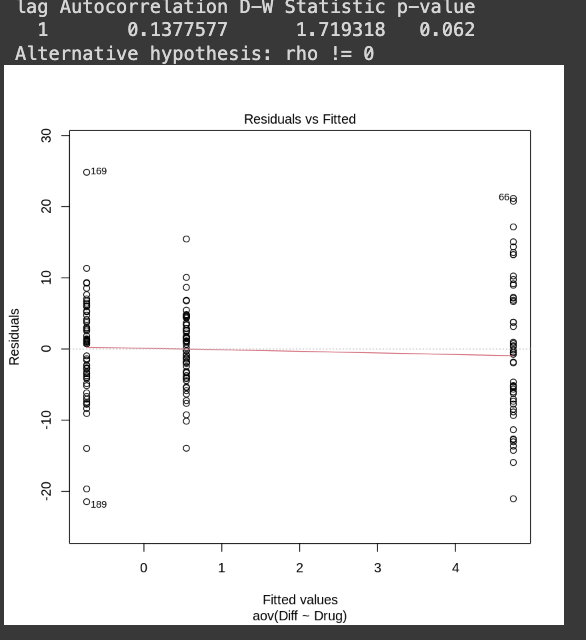
\includegraphics[width=0.8\linewidth]{part01_figures/37.png}
    \caption{Kiểm định tính độc lập của phần dư}
    \label{fig:Kiểm định tính độc lập của phần dư__}
\end{figure}
    Với các giả định:
    \begin{itemize}
        \item H0: Không có sự tương quan (độc lập)
        \item H1: Có sự tương quan (không độc lập)
    \end{itemize}
    Nhận xét: Với giá trị p-value = 0.062 nên không có sự tương quan (trước đó là tương quan dương).

\begin{lstlisting}
# Kiểm định độ hiệu quả trung bình giữa các nhóm thuốc
with(rm_outliner_islander, pairwise.t.test(Diff, Drug, p.adj = "bonferroni"))
TukeyHSD(aov(Diff~Drug, data=rm_outliner_islander), conf.level = 0.95)
plot(TukeyHSD(aov(Diff~Drug, data=rm_outliner_islander), conf.level = 0.95))
\end{lstlisting}
    Với các giả định:
    \begin{itemize}
        \item H0: Các giá trị trung bình giữa các cặp bằng nhau
        \item H1: Các giá trị trung bình giữa các cặp không bằng nhau
    \end{itemize}
    Nhận xét: \begin{itemize}
        \item Nhìn vào kết quả ta có: Nhóm T-S có p-value > 0.05 nên không đủ bác bỏ H0, vậy nhóm này có giá trị trung bình bằng nhau; Các nhóm còn lại p-value đều có giá trị nhỏ hơn 0.05 (độ tin cậy 95\%) nên ta có cơ sở để bác bỏ H0. Vậy rõ ràng giữa các nhóm này có giá trị trung bình là khác nhau.
        \item Nhìn vào kết quả và hình vẽ ta cũng thấy ngay giữa nhóm S-A và T-A có mức độ hiệu quả trung bình khác nhau, T-S có mức độ hiệu quả trung bình như nhau (đồ thị cắt điểm 0) (giống kết quả phân tích trước đó).
        \item \textbf{Kết luận}: \textbf{các tính chất kiểm định về chuẩn cho đánh giá ANOVA và kiểm định ảnh hưởng chính đã cho kết quả tốt hơn so với trước khi chưa xử lý dữ liệu.}
    \end{itemize}
    \item \textbf{Bước 4: Xây dựng và kiểm định mô hình cộng (Additive model)}
    \begin{lstlisting}
add_model = lm(Diff~., data=rm_outliner_islander)
add_model <- MASS::stepAIC(add_model, k = log(nrow(rm_outliner_islander)), trace = 0)
summary(add_model)
add_model$coefficients
    \end{lstlisting}
    Kết quả:
    \begin{lstlisting}

Call:
lm(formula = Diff ~ Drug, data = rm_outliner_islander)

Residuals:
     Min       1Q   Median       3Q      Max 
-21.4645  -4.4450   0.3569   4.3550  24.8355 

Coefficients:
            Estimate Std. Error t value Pr(>|t|)    
(Intercept)   1.5176     0.5785   2.623 0.009502 ** 
Drug1         3.2256     0.8428   3.827 0.000182 ***
Drug2        -0.9726     0.8087  -1.203 0.230799    
---
Signif. codes:  0 '***' 0.001 '**' 0.01 '*' 0.05 '.' 0.1 ' ' 1

Residual standard error: 7.581 on 170 degrees of freedom
Multiple R-squared:  0.08396,	Adjusted R-squared:  0.07318 
F-statistic: 7.791 on 2 and 170 DF,  p-value: 0.000579

(Intercept)
    1.51755112797807
Drug1
    3.22558612692389
Drug2
    -0.972551127978073

    \end{lstlisting}
    Nhận xét: Với p-value=5\%, chỉ có biến Drug có ý nghĩ trong việc giải thích mô hình. như vậy việc kiểm định mô hình cộng giống như phân tích ảnh hưởng chính của biến Drug

Như vậy, mô hình cộng được xây dựng như sau:

\textbf{Diff=1.517 + 3.225×Drug1 - 0.972×Drug2}

- Drug1: Hệ số cho Drug1 là 3.2256. Điều này cho thấy rằng khi sử dụng loại thuốc thứ nhất, sự khác biệt trong thời gian hoàn thành bài kiểm tra tăng thêm
3.2256 iây so với không sử dụng thuốc. Hệ số này có ý nghĩa thống kê (p-value = 0.000182 < 0.001)
- Drug2:Hệ số cho Drug2 là -0.9726. Điều này cho thấy rằng khi sử dụng loại thuốc thứ hai, sự khác biệt trong thời gian hoàn thành bài kiểm tra giảm đi
0.9726 giây so với không sử dụng thuốc. Tuy nhiên, hệ số này không có ý nghĩa thống kê (p-value = 0.230799 > 0.05).
- Mô hình tổng thể có ý nghĩa: F-statistic cho thấy mô hình tổng thể có ý nghĩa thống kê, tuy nhiên, Multiple R-squared thấp cho thấy mô hình chỉ giải thích được một phần nhỏ sự biến thiên của Diff

Kết luận: Nếu xem bản thân loại thuốc và liều thuốc tương tác một cách độc lập, thì sau đây là khuyến nghị cho bác sỹ:
Nên sử dụng loại thuốc 2 (thuốc S) cho bệnh nhân.
Thực tế thì việc sử dụng thuốc cần đánh giá ở nhiều khía cạnh (ví dụ như phân tích ảnh hưỏng đơn cho thấy tương tác mạnh với liều lượng) Vì vậy, cần phải cẩn thận cân nhắc khi sử dụng thuốc tránh đem lại hậu quả không mong muốn ngoài tầm kiểm soát.

\textbf{Như vậy về tổng thể sao khi loại bỏ các điểm ngoại lai và cực ngoại lai, về vieeck thống kê và phân tích ANOVA đã cho ra một mô hình có các yếu tố thỏa mãn các yếu tố kiểm định về chuẩn hơn, trong TH không chuẩn nhưng chỉ số so với trước là tốt hơn}
\end{itemize}

    \section{Phân tích phim truyền thông và xã hội}

\subsection{Giới thiệu chung}

Trong những năm gần đây, các nhà phân tích và nhà đầu tư ngày càng quan tâm đến việc đánh giá rủi ro tài chính trong sản xuất phim. Nghiên cứu này sử dụng phân tích hồi quy tuyến tính bội để dự đoán thành công về mặt tài chính của phim và nghiên cứu mối quan hệ giữa số lần chiếu và năm.

\subsection{Phát biểu bài toán}

Mục tiêu chính của phần này là khám phá và phân tích tổng doanh thu của phim trong hai năm 2014 và 2015 cũng như kiểm tra mối quan hệ và ý nghĩa của một số biến giải thích. Hơn nữa, đồ án xây dựng một mô hình hồi quy tối ưu để đưa ra dự đoán về sự thành công về mặt tài chính, tức là tổng doanh thu của một bộ phim trong hai năm 2014 và 2015. 


\subsection{Giới thiệu về dữ liệu}

Bộ dữ liệu phim truyền thông và xã hội (conventional and social media dataset) được sử dụng trong đồ án này có cấu trúc tương đối đơn giản mà một số người có ích kiến thức về phim truyền hình cũng có thể hiểu được. Vấn đề chính của bộ dữ liệu là missing values, và chúng tôi sẽ cố gắng xử lý nó bằng một số kỹ thuật đã biết.

Ngành công nghiệp điện ảnh là một ngành đóng góp đáng kể cho nền kinh tế của một quốc gia và là một nhà tuyển dụng lớn tại Hoa Kỳ. Do chi phí lớn liên quan đến sản xuất phim, các nhà phân tích cần nghiên cứu và hiểu các biến số chính góp phần vào thành công về mặt thương mại và tài chính của một bộ phim. Đồ án có thể cung cấp thông tin chi tiết về các tính năng chính góp phần vào thành công về mặt tài chính của các bộ phim và thúc đẩy nghiên cứu trong tương lai để xem xét mối quan hệ giữa các biến giải thích đặc biệt độc đáo trong tập dữ liệu. Hơn nữa nó còn có thể giúp các nhà sản xuất phim xác định những tính năng nào cần tập trung vào trong giai đoạn quảng bá để cải thiện thành công của bộ phim.


\subsection{Khám phá và tiền xử lý dữ liệu}


\subsubsection{Đọc dữ liệu và một số kiểm tra khởi đầu}

Trước hết, ta đọc dữ liệu

\begin{lstlisting}
# Đọc dữ liệu từ tập tin
raw_data = read_excel("../../data/part1/CSM.xlsx", sheet = 1)
str(raw_data)

# Thay đổi tên biến `Aggregate Followers` thành `AggregateFollowers`
names(raw_data)[names(raw_data) == 'Aggregate Followers'] <- 'AggregateFollowers'
\end{lstlisting}

Dữ liệu này không có hiện tượng trùng lặp. Dựa trên thông tin của tập dữ liệu, ta thấy mỗi dòng mang ý nghĩa khác nhau, tức là mỗi quan trắc độc lập nhau. Ý nghĩa từng cột như sau:
\begin{itemize}
    \item \textbf{Movie}: tên phim
    \item \textbf{Year}: năm phát hành
    \item \textbf{Ratings}: điểm đánh giá
    \item \textbf{Genre}: thể loại phim
    \item \textbf{Gross}: tổng doanh thu
    \item \textbf{Budget}: tổng chi phí
    \item \textbf{Screens}: số rạp chiều
    \item \textbf{Sequel}: phần phim
    \item \textbf{Sentiment}: ý kiến khán giả
    \item \textbf{Views}: số lượt xem
    \item \textbf{Likes}: số lượt thích
    \item \textbf{Dislikes}: số lượt chê
    \item \textbf{Comments}: số bình luận
    \item \textbf{Aggregate Followers}: số người theo dõi
\end{itemize}

Ta thấy biến Dislikes thể hiện ý nghĩa tương tự biến Likes nhưng có chiều hướng ngược lại. Nên ta có thể loại bỏ biến này khỏi tập dữ liệu.

\subsubsection{Các cột với kiểu dữ liệu số phân bố như thế nào?}

Ta kiểm tra một số thông tin thống kê mô tả của bộ dữ liệu

\begin{minted}{R}
# A tibble: 12 × 7
   variable           missing     min      lower     median      upper       max
   <chr>                <dbl>   <dbl>      <dbl>      <dbl>      <dbl>     <dbl>
 1 Year                   0    2014       2014       2014       2015      2.02e3
 2 Ratings                0       3.1        5.8        6.5        7.1    8.7 e0
 3 Gross                  0    2470   10300000   37400000   89350000      6.43e8
 4 Budget                 0.4 70000    9000000   28000000   65000000      2.5 e8
 5 Screens                4.3     2        449       2777       3372      4.32e3
 6 Sequel                 0       1          1          1          1      7   e0
 7 Sentiment              0     -38          0          0          5.5    2.9 e1
 8 Views                  0     698     623302    2409338    5217380.     3.26e7
 9 Likes                  0       1       1776.      6096      15248.     3.71e5
10 Dislikes               0       0        106.       341        698.     1.40e4
11 Comments               0       0        248.       837       2137      3.84e4
12 AggregateFollowers    15.2  1066     183025    1052600    3694500      3.10e7
\end{minted}
Nhận xét:
\begin{itemize}
    \item Có hiện tượng missing values đối với cột AggregateFollowers, Screens và Budget. Cụ thể, ta thấy biến Aggregate Followers có tỷ lệ missing 15.2\%, biến Screens có tỷ lệ 4.3\% và biến Budget có tỷ lệ missing 0.4\%.
    \item  Có những bộ phim không có likes/ dislikes/ comments, ta sẽ loại bỏ những dòng này.
\end{itemize}

\subsubsection{Các cột với kiểu dữ liệu phân loại phân bố như thế nào?}

Khảo sát cột Genre thể hiện các thể loại phim, ta trực quan bằng biểu đổ tròn dưới đây.

\begin{figure}[H]
    \centering
    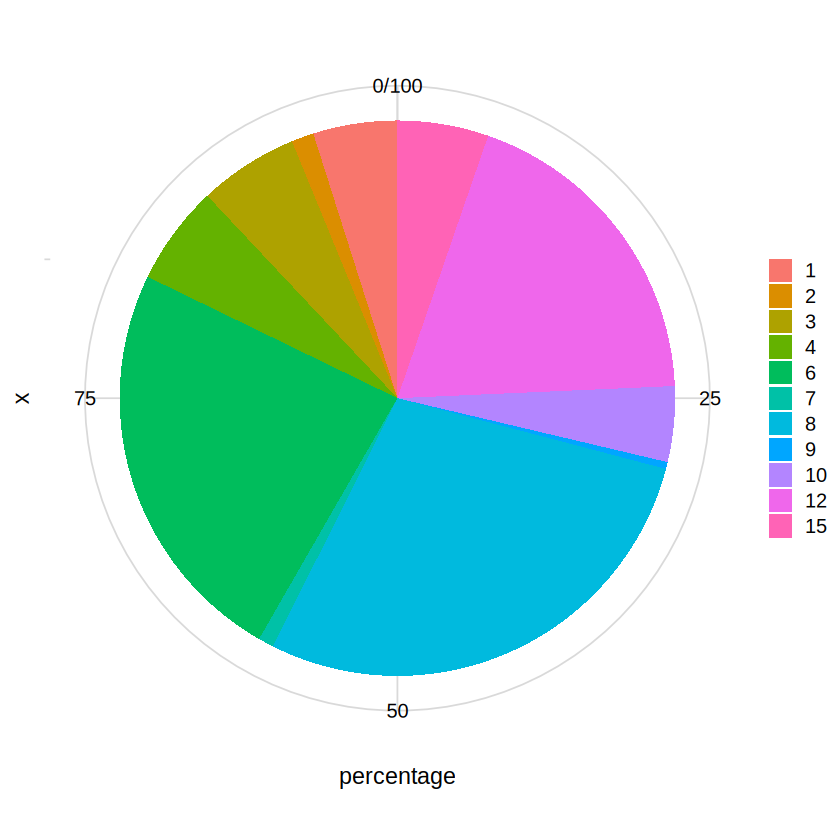
\includegraphics[width=0.75\columnwidth]{csm_figures/genre_part01.png}
    \caption{Tỷ lệ các thể loại phim.}
    \label{fig:genre}
\end{figure}
Nhận xét:
\begin{itemize}
    \item Các thể loại phim phân bố không đều nhau
    \item 
\end{itemize}

\subsubsection{Xử lý dữ liệu bị thiếu}

Trong đồ án này, chúng tôi khảo sát nhiều phương pháp xử lý dữ liệu bị thiếu như sau:
\begin{itemize}
    \item Chèn không (zeros imputed)
    \item Chèn trung bình (means imputed)
    \item Chèn trung vị (median imputed)
    \item Điền các giá trị bị thiếu dựa trên PCA (imputed PCA)
\end{itemize}

Dựa trên kết quả thực nghiệm, chúng tôi chọn điền các giá trị bị thiếu dựa trên PCA vì có kết quả xây dựng mô hình tốt. Chi tiết các kỹ thuật khác được trình bày trong các file code.

Các bước thực hiện điền các giá trị bị thiếu dựa trên PCA:
\begin{itemize}
    \item Bước 1: ước lượng số thành phần chính
\begin{lstlisting}
# Ước lượng thành phần chính
nPCs <- estim_ncpPCA(raw_data[, -c(1)])
print(nPCs)
\end{lstlisting}
    \item Bước 2: điền các giá trị bị thiếu
\begin{lstlisting}
# Xử lý missing value
processed_data <- imputePCA(raw_data[, -c(1)], ncp = nPCs$ncp, scale = TRUE)
processed_data <- processed_data$completeObs
\end{lstlisting}
\end{itemize}

Đánh giá kết quả bằng cách trực quan hóa phân phối trước và sau khi thực hiện việc điền các giá trị bị thiếu:
\begin{lstlisting}
# Trực quan phân phối trước và sau khi fill missing value

h1 <- ggplot(raw_data, aes(x = Budget)) +
  geom_histogram(fill = "#15ad4f", color = "#000000", position = "identity") +
  ggtitle("Budget Original distribution") +
  theme_classic()
h2 <- ggplot(raw_data, aes(x = Screens)) +
  geom_histogram(fill = "#1543ad", color = "#000000", position = "identity") +
  ggtitle("Screens Original distribution") +
  theme_classic()
h3 <- ggplot(raw_data, aes(x = AggregateFollowers )) +
  geom_histogram(fill = "#ad8415", color = "#000000", position = "identity") +
  ggtitle("AggregateFollowers Original distribution") +
  theme_classic()

  
h4 <- ggplot(processed_data, aes(x = Budget)) +
  geom_histogram(fill = "#15ad4f", color = "#000000", position = "identity") +
  ggtitle("Budget PCA-filled distribution") +
  theme_classic()
h5 <- ggplot(processed_data, aes(x = Screens)) +
  geom_histogram(fill = "#1543ad", color = "#000000", position = "identity") +
  ggtitle("Screens PCA-filled distribution") +
  theme_classic()
h6 <- ggplot(processed_data, aes(x = AggregateFollowers )) +
  geom_histogram(fill = "#ad8415", color = "#000000", position = "identity") +
  ggtitle("AggregateFollowers PCA-filled distribution") +
  theme_classic()

plot_grid(h1, h2, h3, h4, h5, h6, nrow = 2, ncol = 3, rel_widths = c(1, 1), rel_heights = c(1, 1))
\end{lstlisting}

\begin{figure}[H]
    \centering
    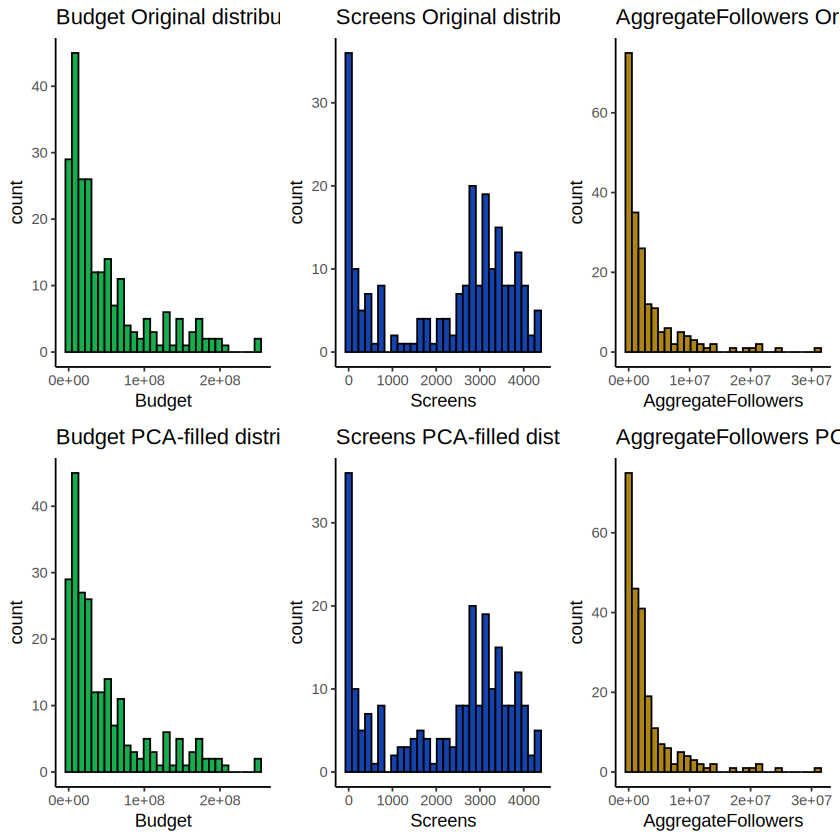
\includegraphics[width=0.75\columnwidth]{csm_figures/imputed_PCA.png}
    \caption{Phân phối trước và sau khi điền các giá trị bị thiếu đối với các cột Budget, Screens và AggregateFollowers.}
    \label{fig:imputed_PCA}
\end{figure}
Nhận xét:
\begin{itemize}
    \item Ta thấy phân phối sau khi điền không có quá nhiều chênh lệch so với phân phối dữ liệu gốc (đã bỏ qua các giá trị bị thiếu)
\end{itemize}

\subsection{Quay lại bước khám phá và tiền xử lý dữ liệu}

Trong phần này, chúng tôi khảo sát các biến để chuẩn hóa dữ liệu. Chúng tôi lựa chọn box-cox transformation để tìm kiếm giá trị $\lambda$ tối ưu để biến đổi dữ liệu.

\subsubsection{Phân tích biến Ratings}

Trong phần này, chúng ta sẽ xem xét biến Ratings thể hiện điểm đánh giá đối với một bộ phim

\begin{figure}[H]
    \centering
    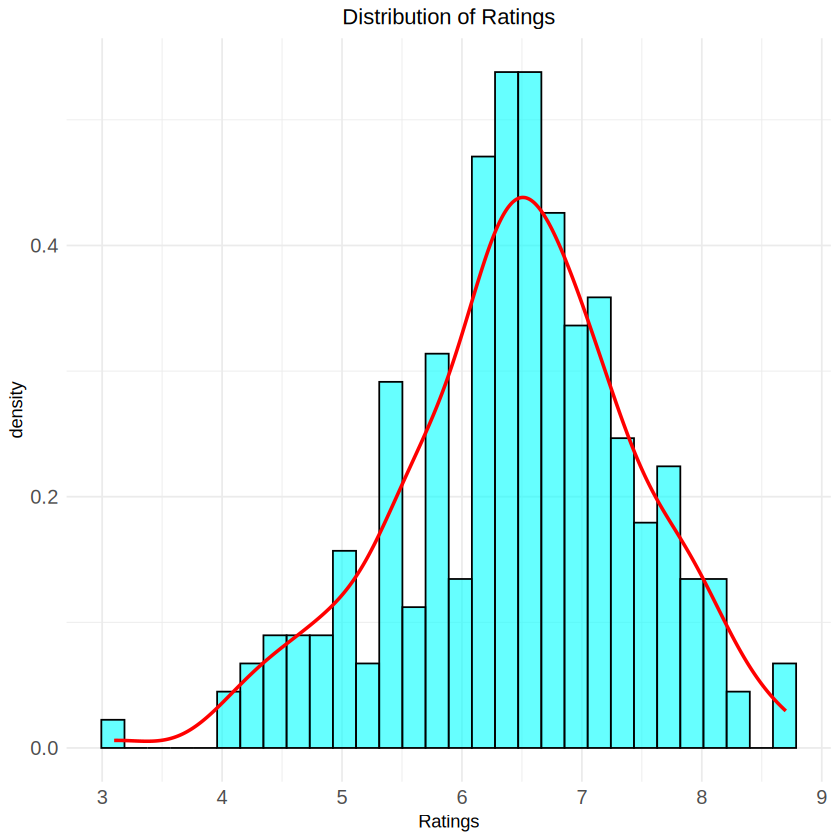
\includegraphics[width=0.75\columnwidth]{csm_figures/ratings_original_distribution.png}
    \caption{Phân phối ban đầu của Ratings.}
    \label{fig:ratings_original_distribution}
\end{figure}

Nhận xét:
\begin{itemize}
    \item Nhìn vào biểu đồ, ta thấy phân phối của biến Ratings tương đối xấp xỉ chuẩn.
\end{itemize}

Ta thử sử dụng log-transform nó và thu được phân phối như hình bên dưới.

\begin{figure}[H]
    \centering
    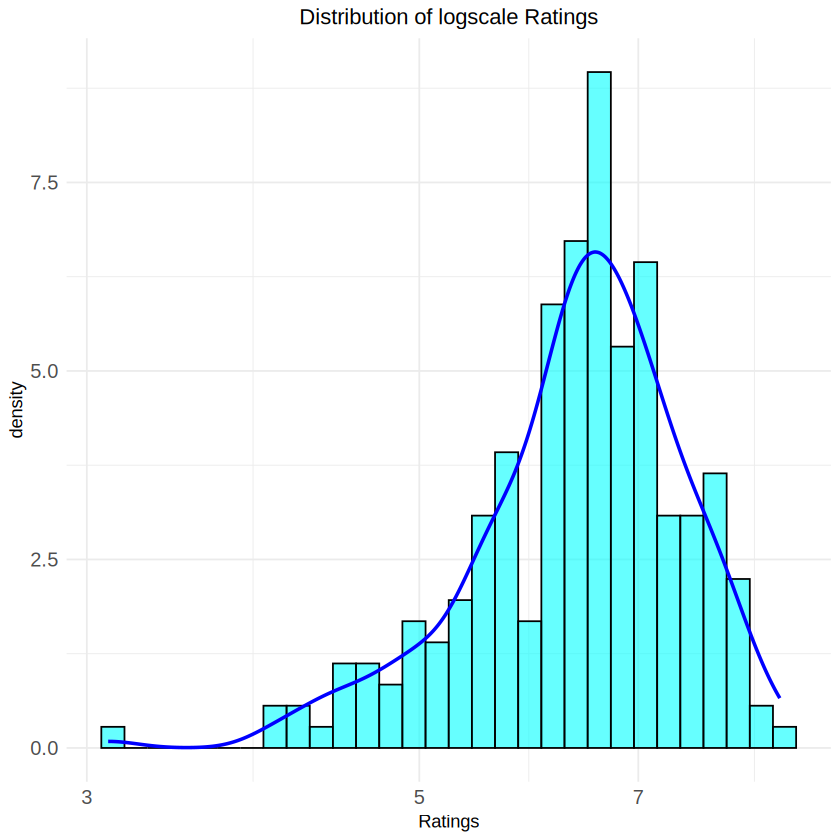
\includegraphics[width=0.75\columnwidth]{csm_figures/ratings_logscale_distribution.png}
    \caption{Phân phối sau khi log-scale của Ratings.}
    \label{fig:ratings_logscale_distribution}
\end{figure}
Nhận xét:
\begin{itemize}
    \item Ta nhận thấy sau khi sử dụng log-transform, dữ liệu bị lệch trái (lệch âm). Do đó, ta thử sử dụng biến đổi box-cox.
\end{itemize}

\begin{figure}[H]
    \centering
    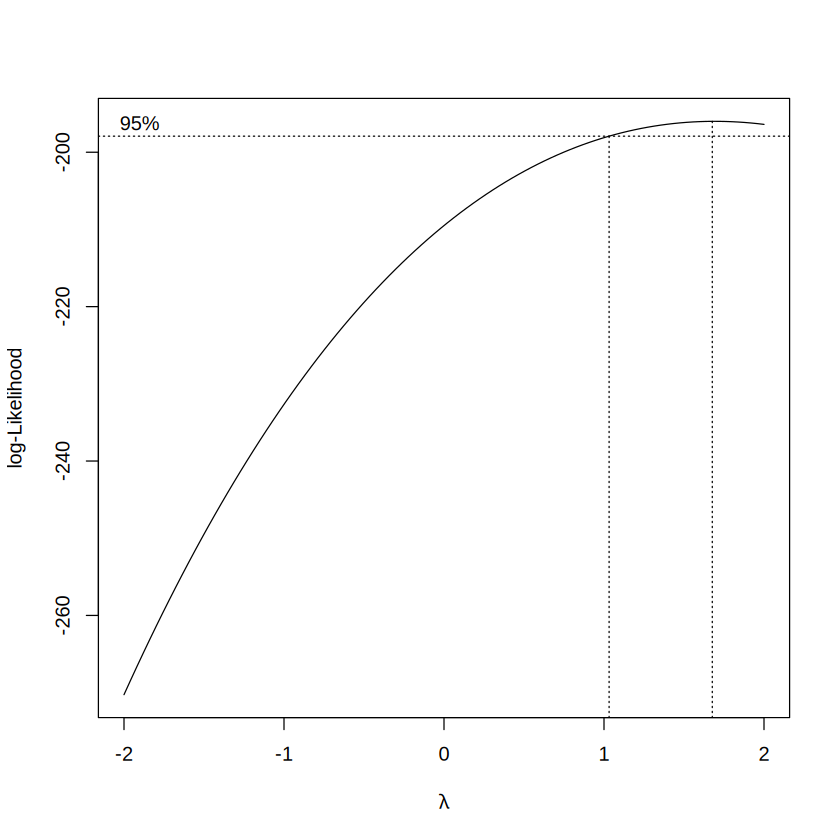
\includegraphics[width=0.75\columnwidth]{csm_figures/ratings_optimal_lambda.png}
    \caption{Log-likelihood với các giá trị $\lambda$ của Ratings.}
    \label{fig:ratings_optimal_lambda}
\end{figure}
Nhận xét:
\begin{itemize}
    \item Dựa trên biểu đồ, ta tìm được giá trị lambda tối ưu với mức ý nghĩa 5\% là 1.677.
\end{itemize}

Và ta thực hiện biến đổi dữ liệu với giá trị lambda vừa tìm được.
\begin{figure}[H]
    \centering
    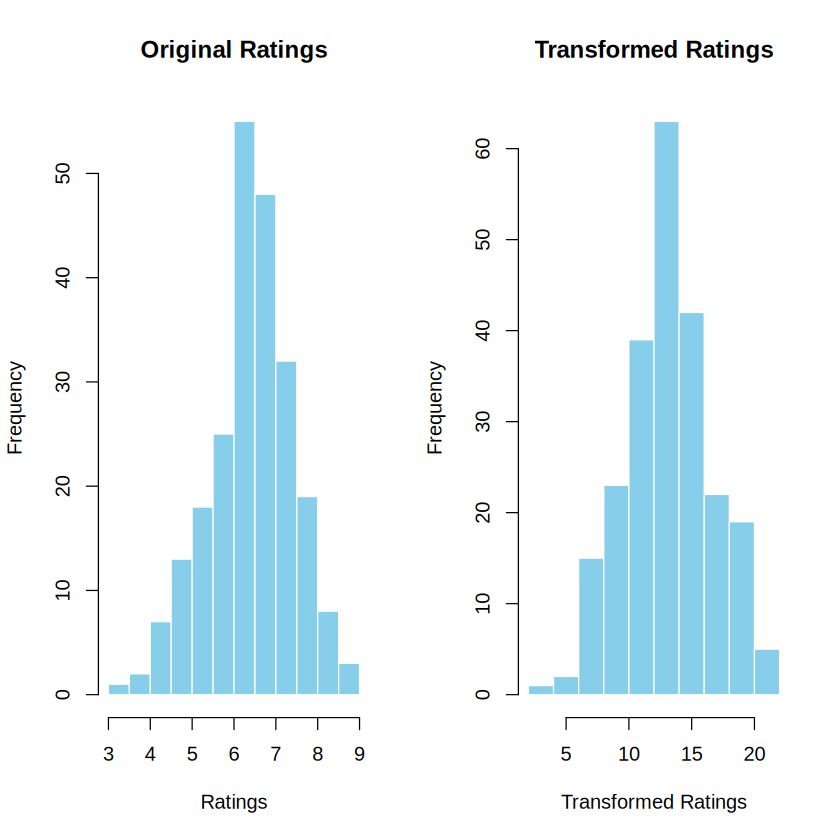
\includegraphics[width=0.75\columnwidth]{csm_figures/ratings_transformed_distribution.png}
    \caption{Phân phối trước và sau khi biến đổi của Gross.}
    \label{fig:ratings_transformed_distribution}
\end{figure}
Nhận xét:
\begin{itemize}
    \item Ta có được giá trị lambda tối ưu là 1.677 và sử dụng giá trị này để biến đổi biến Ratings. Biểu đồ histogram phía bên dưới thể hiện phân phối của biến này trước và sau khi biến đổi. Dễ dàng thấy được, sau khi biến đổi, biến này đã tương đối chuẩn hơn.
\end{itemize}

\subsubsection{Phân tích biến Budget}

Trong phần này, chúng ta sẽ xem xét biến Budget thể hiện chi phí đầu tư cho một bộ phim.

\begin{figure}[H]
    \centering
    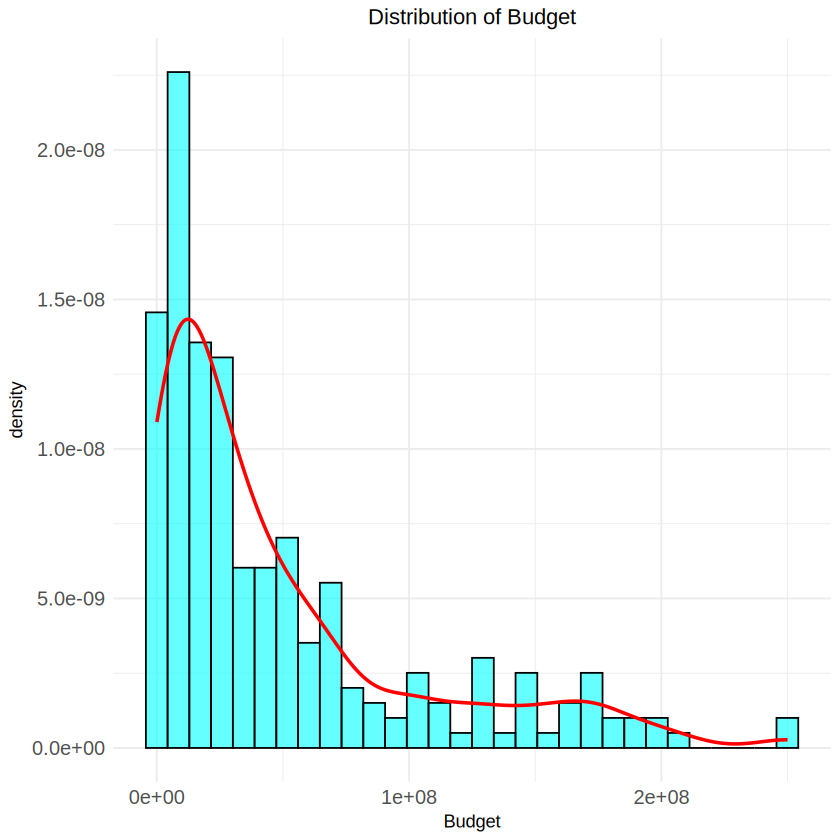
\includegraphics[width=0.75\columnwidth]{csm_figures/budget_original_distribution.png}
    \caption{Phân phối ban đầu của Budget.}
    \label{fig:budget_original_distribution}
\end{figure}

Nhận xét:
\begin{itemize}
    \item Nhìn vào biểu đồ, ta thấy phân phối của biến Ratings bị lệch phải (lệch dương).
\end{itemize}

Ta thử sử dụng log-transform nó và thu được phân phối như hình bên dưới.

\begin{figure}[H]
    \centering
    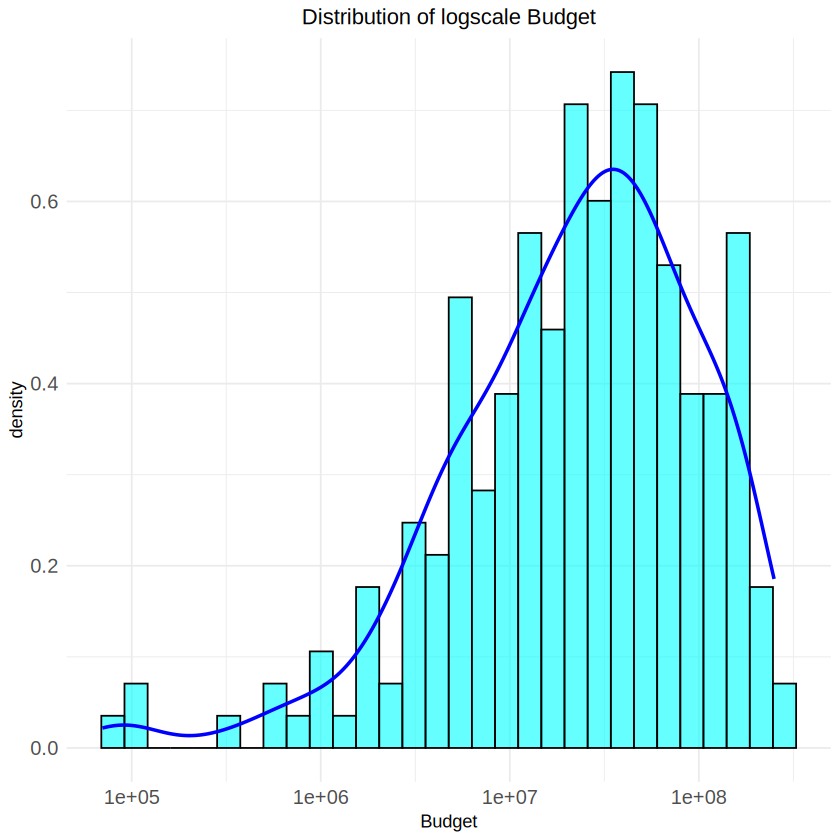
\includegraphics[width=0.75\columnwidth]{csm_figures/budget_logscale_distribution.png}
    \caption{Phân phối sau khi log-scale của Budget.}
    \label{fig:budget_logscale_distribution}
\end{figure}
Nhận xét:
\begin{itemize}
    \item Ta nhận thấy sau khi sử dụng log-transform, dữ liệu tương đối xấp xỉ chuẩn. Do đó, ta thử sử dụng biến đổi box-cox.
\end{itemize}

\begin{figure}[H]
    \centering
    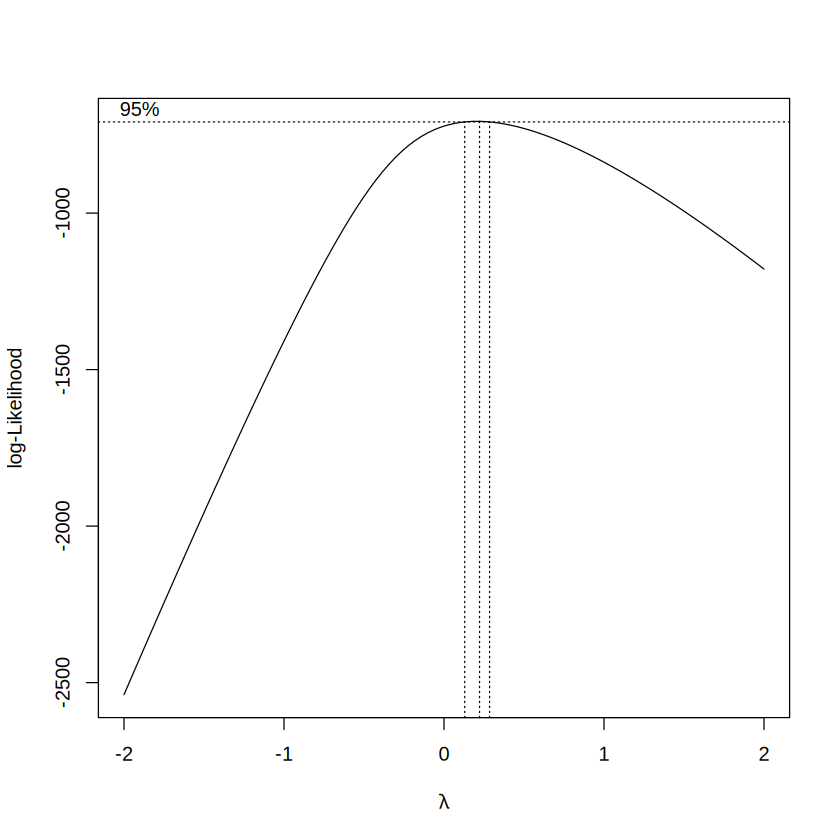
\includegraphics[width=0.75\columnwidth]{csm_figures/budget_optimal_lambda.png}
    \caption{Log-likelihood với các giá trị $\lambda$ của Budget.}
    \label{fig:budget_optimal_lambda}
\end{figure}
Nhận xét:
\begin{itemize}
    \item Dựa trên biểu đồ, ta tìm được giá trị lambda tối ưu với mức ý nghĩa 5\% là 0.222.
\end{itemize}

Và ta thực hiện biến đổi dữ liệu với giá trị lambda vừa tìm được.
\begin{figure}[H]
    \centering
    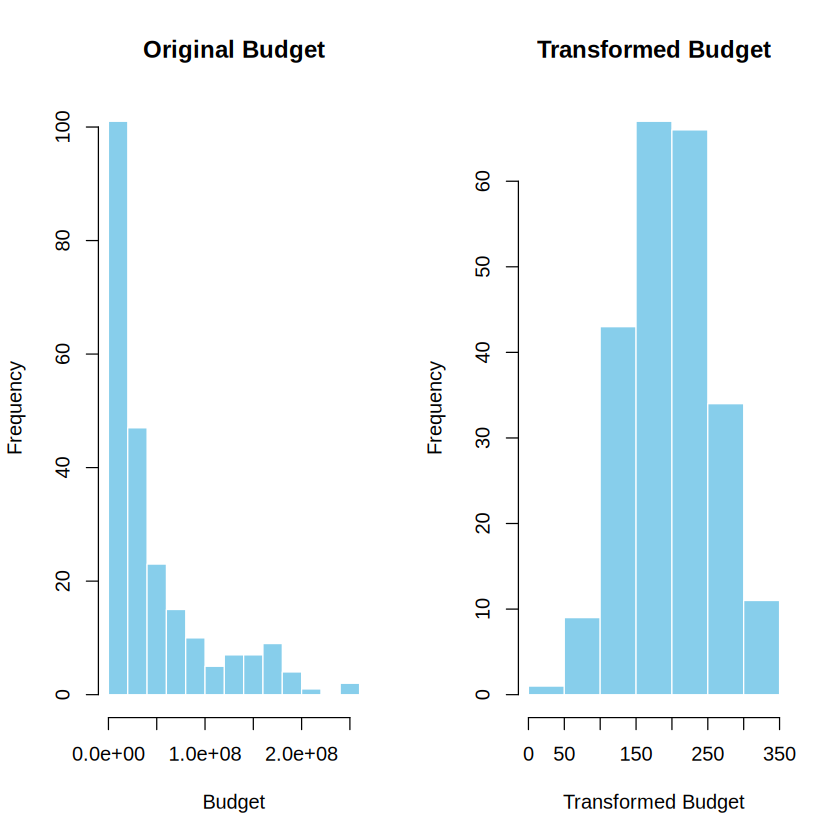
\includegraphics[width=0.75\columnwidth]{csm_figures/budget_transformed_distribution.png}
    \caption{Phân phối trước và sau khi biến đổi của Budget.}
    \label{fig:budget_transformed_distribution}
\end{figure}
Nhận xét:
\begin{itemize}
    \item Ta có được giá trị lambda tối ưu là 0.2222 và sử dụng giá trị này để biến đổi biến Budget. Biểu đồ histogram phía bên dưới thể hiện phân phối của biến này trước và sau khi biến đổi. Dễ dàng thấy được, sau khi biến đổi, biến này đã tương đối chuẩn hơn.
\end{itemize}

\subsubsection{Phân tích biến Screens}

Trong phần này, chúng ta sẽ xem xét biến Screens thể hiện số rạp chiếu của một bộ phim.

\begin{figure}[H]
    \centering
    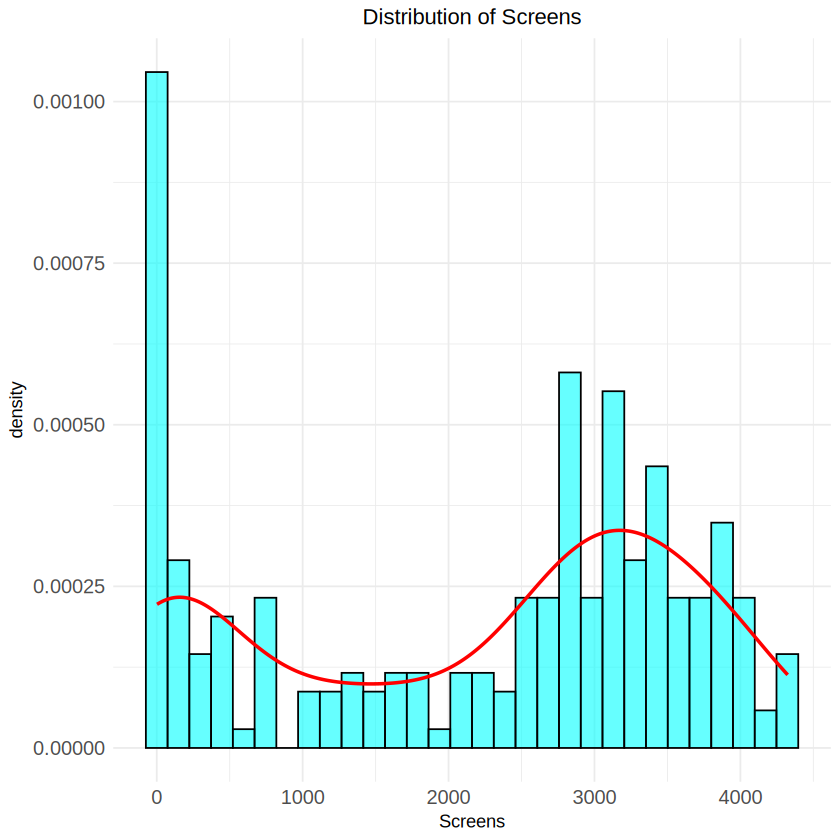
\includegraphics[width=0.75\columnwidth]{csm_figures/screens_original_distribution.png}
    \caption{Phân phối ban đầu của Screens.}
    \label{fig:screens_original_distribution}
\end{figure}

Nhận xét:
\begin{itemize}
    \item Nhìn vào biểu đồ, ta thấy phân phối của biến Screens có phân phối hai đỉnh, trong đó một đỉnh tập trung ở gần 0 và một đỉnh tập trung ở 3000.
\end{itemize}

Ta thử sử dụng log-transform nó và thu được phân phối như hình bên dưới.

\begin{figure}[H]
    \centering
    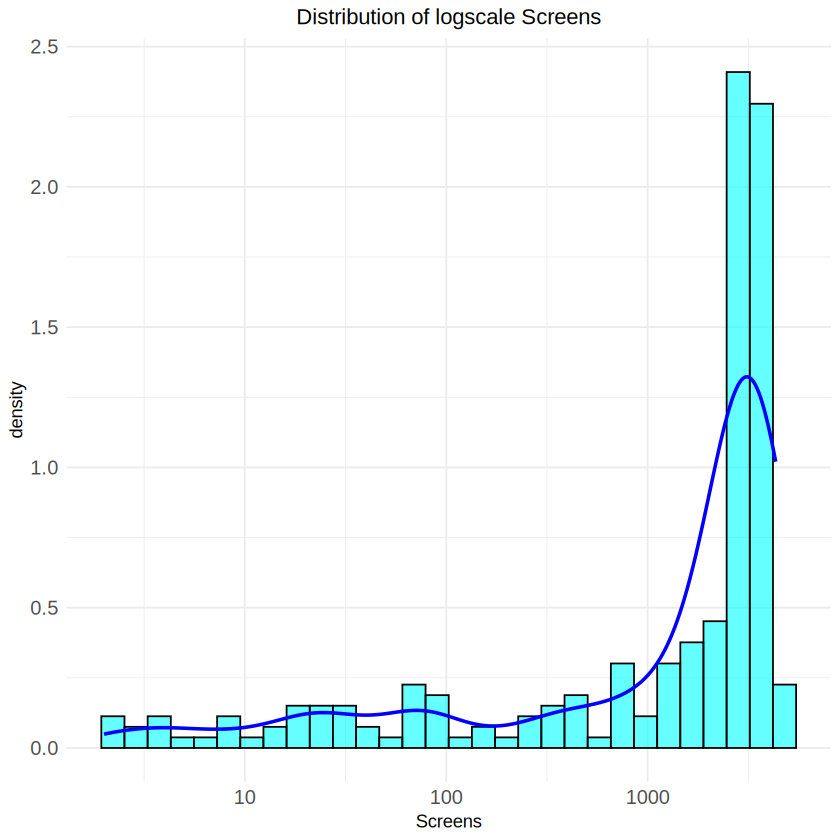
\includegraphics[width=0.75\columnwidth]{csm_figures/screens_logscale_distribution.png}
    \caption{Phân phối sau khi log-scale của Screens.}
    \label{fig:screens_logscale_distribution}
\end{figure}
Nhận xét:
\begin{itemize}
    \item Ta nhận thấy sau khi sử dụng log-transform, dữ liệu tương đối bị lệch phải (lệch dương). Do đó, ta thử sử dụng biến đổi box-cox.
\end{itemize}

\begin{figure}[H]
    \centering
    \includegraphics[width=0.75\columnwidth]{csm_figures/budget_optimal_lambda.png}
    \caption{Log-likelihood với các giá trị $\lambda$ của Screens.}
    \label{fig:screens_optimal_lambda}
\end{figure}
Nhận xét:
\begin{itemize}
    \item Dựa trên biểu đồ, ta tìm được giá trị lambda tối ưu với mức ý nghĩa 5\% là 0.5858.
\end{itemize}

Và ta thực hiện biến đổi dữ liệu với giá trị lambda vừa tìm được.
\begin{figure}[H]
    \centering
    \includegraphics[width=0.75\columnwidth]{csm_figures/screens_transformed_distribution.png}
    \caption{Phân phối trước và sau khi biến đổi của Screens.}
    \label{fig:screens_transformed_distribution}
\end{figure}
Nhận xét:
\begin{itemize}
    \item Ta có được giá trị lambda tối ưu là 0.2222 và sử dụng giá trị này để biến đổi biến Screens. Biểu đồ histogram phía bên dưới thể hiện phân phối của biến này trước và sau khi biến đổi. Dễ dàng thấy được, sau khi biến đổi, biến này vẫn có phân phối hai đỉnh trong đó một đỉnh tập trung ở gần 0 còn đỉnh còn lại tập trung ở 200.
    \item Như vậy, có thể có ngoại lai xuất hiện, ta cần thực hiện loại bỏ các cực ngoại lai để tiếp tục xây dựng môn hình.
\end{itemize}

\subsubsection{Phân tích biến Sequel}

Trong phần này, chúng ta sẽ xem xét biến Sequel thể hiện các phần của một bộ phim.

\begin{figure}[H]
    \centering
    \includegraphics[width=0.75\columnwidth]{csm_figures/sequel_original_distribution.png}
    \caption{Phân phối ban đầu của Sequel.}
    \label{fig:sequel_original_distribution}
\end{figure}

Nhận xét:
\begin{itemize}
    \item Nhìn vào biểu đồ, ta thấy phân phối của biến Ratings bị lệch trái (lệch âm).
    \item Đa số các bộ phim chỉ có một phần phim
    \item Rất ít các bộ phim có từ 4 phần trở lên
    \item Số lượng các bộ phim có 5 phần nhiều hơn các bộ phim có 4 phần, và 6 phần
\end{itemize}

\subsubsection{Phân tích biến Sentiment}

Trong phần này, chúng ta sẽ xem xét biến Sentiment thể hiện ý kiến khán giả đối với một bộ phim.

\begin{figure}[H]
    \centering
    \includegraphics[width=0.75\columnwidth]{csm_figures/sentiment_original_distribution.png}
    \caption{Phân phối ban đầu của Sentiment.}
    \label{fig:sentiment_original_distribution}
\end{figure}

Nhận xét:
\begin{itemize}
    \item Nhìn vào biểu đồ, ta thấy phân phối của biến Sentiment có phân phối xấp xỉ chuẩn.
    \item Tuy nhiên, các giá trị tập trung ở 0 rất cao.
\end{itemize}

Ta thử sử dụng log-transform nó và thu được phân phối như hình bên dưới.

\begin{figure}[H]
    \centering
    \includegraphics[width=0.75\columnwidth]{csm_figures/sentiment_logscale_distribution.png}
    \caption{Phân phối sau khi log-scale của Sentiment.}
    \label{fig:sentiment_logscale_distribution}
\end{figure}
Nhận xét:
\begin{itemize}
    \item Ta nhận thấy sau khi sử dụng log-transform, dữ liệu tương đối lệch trái (lệch dương). Do đó, ta thử sử dụng biến đổi box-cox.
\end{itemize}

\begin{figure}[H]
    \centering
    \includegraphics[width=0.75\columnwidth]{csm_figures/sentiment_optimal_lambda.png}
    \caption{Log-likelihood với các giá trị $\lambda$ của Sentiment.}
    \label{fig:sentiment_optimal_lambda}
\end{figure}
Nhận xét:
\begin{itemize}
    \item Dựa trên biểu đồ, ta tìm được giá trị lambda tối ưu với mức ý nghĩa 5\% là 1.111.
\end{itemize}

Và ta thực hiện biến đổi dữ liệu với giá trị lambda vừa tìm được.
\begin{figure}[H]
    \centering
    \includegraphics[width=0.75\columnwidth]{csm_figures/sentiment_transformed_distribution.png}
    \caption{Phân phối trước và sau khi biến đổi của Sentiment.}
    \label{fig:sentiment_transformed_distribution}
\end{figure}
Nhận xét:
\begin{itemize}
    \item Ta có được giá trị lambda tối ưu là 1.11 và sử dụng giá trị này để biến đổi biến Sentiment. Biểu đồ histogram phía bên dưới thể hiện phân phối của biến này trước và sau khi biến đổi. Dễ dàng thấy được, sau khi biến đổi, biến này đã tương đối chuẩn hơn.
\end{itemize}

\subsubsection{Phân tích biến Views}

Trong phần này, chúng ta sẽ xem xét biến Views thể hiện số lượt xem của một bộ phim.

\begin{figure}[H]
    \centering
    \includegraphics[width=0.75\columnwidth]{csm_figures/views_original_distribution.png}
    \caption{Phân phối ban đầu của Views.}
    \label{fig:views_original_distribution}
\end{figure}

Nhận xét:
\begin{itemize}
    \item Nhìn vào biểu đồ, ta thấy phân phối của biến Views có phân phối bị lệch trái (lệch dương).
\end{itemize}

Ta thử sử dụng log-transform nó và thu được phân phối như hình bên dưới.

\begin{figure}[H]
    \centering
    \includegraphics[width=0.75\columnwidth]{csm_figures/views_logscale_distribution.png}
    \caption{Phân phối sau khi log-scale của Views.}
    \label{fig:views_logscale_distribution}
\end{figure}
Nhận xét:
\begin{itemize}
    \item Ta nhận thấy sau khi sử dụng log-transform, dữ liệu tương đối lệch phải (lệch âm). Do đó, ta thử sử dụng biến đổi box-cox.
\end{itemize}

\begin{figure}[H]
    \centering
    \includegraphics[width=0.75\columnwidth]{csm_figures/views_optimal_lambda.png}
    \caption{Log-likelihood với các giá trị $\lambda$ của Views.}
    \label{fig:views_optimal_lambda}
\end{figure}
Nhận xét:
\begin{itemize}
    \item Dựa trên biểu đồ, ta tìm được giá trị lambda tối ưu với mức ý nghĩa 5\% là 0.2626.
\end{itemize}

Và ta thực hiện biến đổi dữ liệu với giá trị lambda vừa tìm được.
\begin{figure}[H]
    \centering
    \includegraphics[width=0.75\columnwidth]{csm_figures/views_transformed_distribution.png}
    \caption{Phân phối trước và sau khi biến đổi của Views.}
    \label{fig:views_transformed_distribution}
\end{figure}
Nhận xét:
\begin{itemize}
    \item Ta có được giá trị lambda tối ưu là 0.2626 và sử dụng giá trị này để biến đổi biến Views. Biểu đồ histogram phía bên dưới thể hiện phân phối của biến này trước và sau khi biến đổi. Dễ dàng thấy được, sau khi biến đổi, biến này đã tương đối chuẩn hơn.
\end{itemize}

\subsubsection{Phân tích biến Likes}

Trong phần này, chúng ta sẽ xem xét biến Likes thể hiện số lượt thích của một bộ phim.

\begin{figure}[H]
    \centering
    \includegraphics[width=0.75\columnwidth]{csm_figures/likes_original_distribution.png}
    \caption{Phân phối ban đầu của Likes.}
    \label{fig:likes_original_distribution}
\end{figure}

Nhận xét:
\begin{itemize}
    \item Nhìn vào biểu đồ, ta thấy phân phối của biến Likes có phân phối bị lệch trái (lệch dương).
\end{itemize}

Ta thử sử dụng log-transform nó và thu được phân phối như hình bên dưới.

\begin{figure}[H]
    \centering
    \includegraphics[width=0.75\columnwidth]{csm_figures/likes_logscale_distribution.png}
    \caption{Phân phối sau khi log-scale của Likes.}
    \label{fig:likes_logscale_distribution}
\end{figure}
Nhận xét:
\begin{itemize}
    \item Ta nhận thấy sau khi sử dụng log-transform, dữ liệu tương đối lệch phải (lệch âm). Do đó, ta thử sử dụng biến đổi box-cox.
\end{itemize}

\begin{figure}[H]
    \centering
    \includegraphics[width=0.75\columnwidth]{csm_figures/likes_optimal_lambda.png}
    \caption{Log-likelihood với các giá trị $\lambda$ của Likes.}
    \label{fig:likes_optimal_lambda}
\end{figure}
Nhận xét:
\begin{itemize}
    \item Dựa trên biểu đồ, ta tìm được giá trị lambda tối ưu với mức ý nghĩa 5\% là 0.2222.
\end{itemize}

Và ta thực hiện biến đổi dữ liệu với giá trị lambda vừa tìm được.
\begin{figure}[H]
    \centering
    \includegraphics[width=0.75\columnwidth]{csm_figures/likes_transformed_distribution.png}
    \caption{Phân phối trước và sau khi biến đổi của Likes.}
    \label{fig:likes_transformed_distribution}
\end{figure}
Nhận xét:
\begin{itemize}
    \item Ta có được giá trị lambda tối ưu là 0.2222 và sử dụng giá trị này để biến đổi biến Likes. Biểu đồ histogram phía bên dưới thể hiện phân phối của biến này trước và sau khi biến đổi. Dễ dàng thấy được, sau khi biến đổi, biến này đã tương đối chuẩn hơn.
\end{itemize}

\subsubsection{Phân tích biến Comments}

Trong phần này, chúng ta sẽ xem xét biến Comments thể hiện số bình luận của một bộ phim.

\begin{figure}[H]
    \centering
    \includegraphics[width=0.75\columnwidth]{csm_figures/comments_original_distribution.png}
    \caption{Phân phối ban đầu của Likes.}
    \label{fig:comments_original_distribution}
\end{figure}

Nhận xét:
\begin{itemize}
    \item Nhìn vào biểu đồ, ta thấy phân phối của biến Comments có phân phối bị lệch trái (lệch dương).
\end{itemize}

Ta thử sử dụng log-transform nó và thu được phân phối như hình bên dưới.

\begin{figure}[H]
    \centering
    \includegraphics[width=0.75\columnwidth]{csm_figures/comments_logscale_distribution.png}
    \caption{Phân phối sau khi log-scale của Comments.}
    \label{fig:comments_logscale_distribution}
\end{figure}
Nhận xét:
\begin{itemize}
    \item Ta nhận thấy sau khi sử dụng log-transform, dữ liệu tương đối lệch phải (lệch âm). Do đó, ta thử sử dụng biến đổi box-cox.
\end{itemize}

\begin{figure}[H]
    \centering
    \includegraphics[width=0.75\columnwidth]{csm_figures/comments_optimal_lambda.png}
    \caption{Log-likelihood với các giá trị $\lambda$ của Comments.}
    \label{fig:comments_optimal_lambda}
\end{figure}
Nhận xét:
\begin{itemize}
    \item Dựa trên biểu đồ, ta tìm được giá trị lambda tối ưu với mức ý nghĩa 5\% là  0.1818.
\end{itemize}

Và ta thực hiện biến đổi dữ liệu với giá trị lambda vừa tìm được.
\begin{figure}[H]
    \centering
    \includegraphics[width=0.75\columnwidth]{csm_figures/comments_transformed_distribution.png}
    \caption{Phân phối trước và sau khi biến đổi của Comments.}
    \label{fig:comments_transformed_distribution}
\end{figure}
Nhận xét:
\begin{itemize}
    \item Ta có được giá trị lambda tối ưu là  0.1818 và sử dụng giá trị này để biến đổi biến Comments. Biểu đồ histogram phía bên dưới thể hiện phân phối của biến này trước và sau khi biến đổi. Dễ dàng thấy được, sau khi biến đổi, biến này đã tương đối chuẩn hơn.
\end{itemize}

\subsubsection{Phân tích biến Gross}

\begin{figure}[H]
    \centering
    \includegraphics[width=0.75\columnwidth]{csm_figures/gross_original_distribution.png}
    \caption{Phân phối ban đầu của Gross.}
    \label{fig:gross_original_distribution}
\end{figure}

Nhận xét:
\begin{itemize}
    \item Nhìn vào biểu đồ, ta thấy phân phối của biến Gross bị lệch trái.
\end{itemize}

Ta thử sử dụng log-transform nó.

\begin{figure}[H]
    \centering
    \includegraphics[width=0.75\columnwidth]{csm_figures/gross_logscale_distribution.png}
    \caption{Phân phối sau khi log-scale của Gross.}
    \label{fig:gross_logscale_distribution}
\end{figure}
Nhận xét:
\begin{itemize}
    \item Ta nhận thấy sau khi sử dụng log-transform, dữ liệu bị lệch phải. Do đó, ta thử sử dụng box-cox.
\end{itemize}

\begin{figure}[H]
    \centering
    \includegraphics[width=0.75\columnwidth]{csm_figures/gross_optimal_lambda.png}
    \caption{Log-likelihood với các giá trị $\lambda$ của Gross.}
    \label{fig:gross_optimal_lambda}
\end{figure}
Nhận xét:
\begin{itemize}
    \item Dựa trên biểu đồ, ta tìm được giá trị lambda tối ưu với mức ý nghĩa 5\% là 0.262
\end{itemize}

Và ta thực hiện biến đổi dữ liệu với giá trị lambda vừa tìm được.
\begin{figure}[H]
    \centering
    \includegraphics[width=0.75\columnwidth]{csm_figures/gross_transformed_distribution.png}
    \caption{Phân phối trước và sau khi biến đổi của Gross.}
    \label{fig:gross_transformed_distribution}
\end{figure}
Nhận xét:
\begin{itemize}
    \item Ta có được giá trị lambda tối ưu là 0.262 và sử dụng giá trị này để biến đổi biến Gross. Biểu đồ histogram phía bên dưới thể hiện phân phối của biến này trước và sau khi biến đổi. Dễ dàng thấy được, sau khi biến đổi, biến này đã tương đối chuẩn hơn.
\end{itemize}

\subsubsection{Phân tích biến AggregateFollowers}

\begin{figure}[H]
    \centering
    \includegraphics[width=0.75\columnwidth]{csm_figures/af_original_distribution.png}
    \caption{Phân phối ban đầu của Gross.}
    \label{fig:af_original_distribution}
\end{figure}
Nhận xét:
\begin{itemize}
    \item Nhìn vào biểu đồ, ta thấy phân phối của biến AggregateFollowers bị lệch phải.
\end{itemize}

\begin{figure}[H]
    \centering
    \includegraphics[width=0.75\columnwidth]{csm_figures/af_logscale_distribution.png}
    \caption{Phân phối sau khi logscale của AggregateFollowers.}
    \label{fig:af_logscale_distribution}
\end{figure}
Nhận xét:
\begin{itemize}
    \item Khi dùng log-scale, phân phối của biến Comments đã xấp xỉ chuẩn hơn.
    \item Ta có thể dùng box-cox để biến đổi dữ liệu nhờ vào việc tìm lambda tối ưu.
\end{itemize}

\begin{figure}[H]
    \centering
    \includegraphics[width=0.75\columnwidth]{csm_figures/af_optimal_lambda.png}
    \caption{Log-likelihood với các giá trị $\lambda$ của AggregateFollowers.}
    \label{fig:af_optimal_lambda}
\end{figure}
Nhận xét:
\begin{itemize}
    \item Dựa trên biểu đồ, ta tìm được giá trị lambda tối ưu với mức ý nghĩa 5\% là 0.182
\end{itemize}

Và ta thực hiện biến đổi dữ liệu với giá trị lambda vừa tìm được.
\begin{figure}[H]
    \centering
    \includegraphics[width=0.75\columnwidth]{csm_figures/af_transformed_distribution.png}
    \caption{Phân phối trước và sau khi biến đổi của AggregateFollowers.}
    \label{fig:af_transformed_distribution}
\end{figure}
Nhận xét:
\begin{itemize}
    \item Ta có được giá trị lambda tối ưu là 0.33 và sử dụng giá trị này để biến đổi biến AggregateFollowers. Biểu đồ histogram phía bên dưới thể hiện phân phối của biến này trước và sau khi biến đổi. Dễ dàng thấy được, sau khi biến đổi, biến này đã tương đối chuẩn hơn.
\end{itemize}

\subsection{Mô hình hóa}

\subsubsection{Xử lý đa cộng tuyến}

Đầu tiên, ta trực quan hóa ma trận tương quan giữa các biến trong tập dữ liệu
\begin{figure}[H]
    \centering
    \includegraphics[width=0.75\columnwidth]{csm_figures/corr.png}
    \caption{Ma trận tương quan giữa các biến trong tập dữ liệu phim truyền thông.}
    \label{fig:csm_corr}
\end{figure}

Nhận xét:
\begin{itemize}
    \item Một số cặp có khả năng đa cộng tuyến cao: Views` và `Comments`, Likes` và `Comments`, `Gross` và `Budget`
    \item Một số cặp tương quan nghịch tương đối vừa: Sequel và Sentiment (-0.11)
\end{itemize}

Ta xử lý đa cộng tuyến thông qua các bước sau. Bước 1: Tính toán chỉ số VIF
\begin{lstlisting}
Ratings             Budget            Screens             Sequel 
          1.196619           2.239092           1.740774           1.406844 
         Sentiment              Views              Likes           Comments 
          1.050186           2.172907           7.324670           7.884851 
AggregateFollowers 
          1.147767 
\end{lstlisting}
Nhận xét:
\begin{itemize}
    \item Ta có chọn ngưỡng bằng 3
\end{itemize}
Bước 2: Loại bỏ các biến dựa trên VIF nếu vượt quá ngưỡng
\begin{lstlisting}
    Ratings             Budget            Screens             Sequel 
          1.152850           2.075596           1.736352           1.362376 
         Sentiment              Views              Likes AggregateFollowers 
          1.050070           2.007632           1.905291           1.129789 

Call:
lm(formula = Gross ~ Ratings + Budget + Screens + Sequel + Sentiment + 
    Views + Likes + AggregateFollowers, data = csm_df)

Residuals:
       Min         1Q     Median         3Q        Max 
-125889542  -27197502   -3079763   16371993  417347246 

Coefficients:
                     Estimate Std. Error t value Pr(>|t|)    
(Intercept)        -1.226e+08  2.671e+07  -4.588 7.50e-06 ***
Ratings             1.590e+07  4.005e+06   3.970 9.73e-05 ***
Budget              7.509e-01  9.803e-02   7.660 5.68e-13 ***
Screens             1.448e+04  3.372e+03   4.294 2.62e-05 ***
Sequel              8.854e+06  4.451e+06   1.989  0.04788 *  
Sentiment          -4.850e+05  5.402e+05  -0.898  0.37022    
Views               4.518e-01  1.158e+00   0.390  0.69692    
Likes               9.093e+01  1.766e+02   0.515  0.60717    
AggregateFollowers  2.494e+00  8.657e-01   2.880  0.00436 ** 
---
Signif. codes:  0 '***' 0.001 '**' 0.01 '*' 0.05 '.' 0.1 ' ' 1

Residual standard error: 55930000 on 222 degrees of freedom
Multiple R-squared:  0.6179,	Adjusted R-squared:  0.6042 
F-statistic: 44.88 on 8 and 222 DF,  p-value: < 2.2e-16
\end{lstlisting}
Như vậy, chúng ta đã thu được tập dữ liệu bao gồm các biến không có đa cộng tuyến với nhau. (Đã loại bỏ được biến comments)

\subsubsection{Khảo sát ngoại lai}

Để loại bỏ những ngoại lại, ta sử dụng IQR để tìm và loại bỏ các điểm cực ngoại lai.

\begin{lstlisting}
# Ở đây sử dụng IQR để loại bỏ ngoại lai
Q1 <- quantile(cleaned_df$'Gross', 0.25)
Q3 <- quantile(cleaned_df$'Gross', 0.75)
IQR <- Q3 - Q1
lower_bound <- Q1 - 1.5 * IQR
upper_bound <- Q3 + 1.5 * IQR
outliers <- which(cleaned_df$'Gross' < lower_bound | cleaned_df$'Gross' > upper_bound)
print(outliers)

lower_bound <- Q1 - 3 * IQR
upper_bound <- Q3 + 3 * IQR
extreme_outliers <- which(cleaned_df$'Gross' < lower_bound | cleaned_df$'Gross' > upper_bound)
print(extreme_outliers)
\end{lstlisting}

Ta thu được các điểm dữ liệu ngoại lai: 11  19  27  28  47  71 125 128 134 151 162 164 165 166 167 168

Các điểm dữ liệu cực ngoại lai: 11  47 128 164 165 166 167

Bằng cách loại bỏ các điểm dữ liệu cực ngoại lai, ta thu được tập dữ liệu để có thể khảo sát tiếp.


\subsubsection{Xây dựng mô hình đầy đủ}

Đầu tiên, ta phân chia tập dữ liệu thành 2 phần: train (80\%) và test (20\%).
\begin{lstlisting}
split_ratio <- 0.8
split_index <- floor(nrow(csm_df) * split_ratio)

train = csm_df[1:split_index,]
test = csm_df[(split_index + 1):nrow(csm_df),]
\end{lstlisting}

Sau đó, ta xây dựng mô hình đầy đủ các biến như sau:

\begin{lstlisting}
full.lm <- lm(Gross ~ ., data = train)
print(summary(full.lm))
\end{lstlisting}

Kết quả

\begin{lstlisting}
lm(formula = Gross ~ ., data = train)

Residuals:
    Min      1Q  Median      3Q     Max 
-136.99  -18.79    3.70   22.97   84.15 

Coefficients:
                    Estimate Std. Error t value Pr(>|t|)    
(Intercept)        -60.21332   62.87576  -0.958   0.3396    
Ratings             21.80737   12.55030   1.738   0.0841 .  
Budget               0.65118    0.08619   7.555 2.46e-12 ***
Screens              2.89668    0.49989   5.795 3.25e-08 ***
Sequel              11.31840    6.07145   1.864   0.0640 .  
Sentiment           -0.21697   10.96256  -0.020   0.9842    
Views               -0.29107    0.25634  -1.136   0.2578    
Likes                1.79341    0.75762   2.367   0.0190 *  
AggregateFollowers   0.03477    0.09788   0.355   0.7228    
---
Signif. codes:  0 '***' 0.001 '**' 0.01 '*' 0.05 '.' 0.1 ' ' 1

Residual standard error: 34.9 on 170 degrees of freedom
Multiple R-squared:  0.6614,	Adjusted R-squared:  0.6455 
F-statistic: 41.51 on 8 and 170 DF,  p-value: < 2.2e-16
\end{lstlisting}
Nhận xét:
\begin{itemize}
    \item Mô hình này có R-squared hiệu chỉnh 0.6455, tức là phương sai biến Gross có thể được giải thích được 64.55\% dựa trên các biến độc lập của mô hình.
    \item Với mức ý nghĩa 5\%, ta thấy các biến Budget, Screen, Ratings, Sequel và Likes có ý nghĩa đối với mô hình
\end{itemize}

\subsubsection{Lựa chọn model tốt nhất}

Với số lượng lớn các yếu tố dự đoán, điều quan trọng là phải giảm thiểu mô hình bằng cách chỉ bao gồm các yếu tố dự đoán hữu ích. Có tất cả 8 yếu tố dự đoán trong tập dữ liệu, nghĩ là có thể có $2^{8}$ mô hình hồi quy. Để chọn mô hình một cách hiệu quả, việc lựa chọn lùi được thực hiện bằng sử dụng step function. Phương pháp này lặp lại các quy trình để giảm thiểu Akaike’s Information Criteria (AIC) và Bayesian Information Criteria (BIC). Lựa chọn mô hình ngược so với lựa chọn tiến vì nó loại bỏ khả năng một yếu tố dự đoán mới được chọn có khả năng tương tự hoặc nhiều hơn để giải thích các phần của phản hồi đã được giải thích bởi một yếu tố dự đoán khác có trong mô hình.

\begin{lstlisting}
# Mô hình chặn dưới
model.lb <- lm(Gross ~ 1, data = train) 

# Mô hình chặn trên
model.up <- full.lm

step(full.lm, scope = list(lower = model.lb, upper = model.up), direction = "both", trace = FALSE)
\end{lstlisting}

Kết quả
\begin{lstlisting}
Call:
lm(formula = Gross ~ Ratings + Budget + Screens + Sequel + Likes, 
    data = train)

Coefficients:
(Intercept)      Ratings       Budget      Screens       Sequel        Likes  
   -72.5562      24.4101       0.6444       2.9817      11.9940       1.0309  
\end{lstlisting}

\begin{lstlisting}
csm_models<- regsubsets(Gross ~  Ratings + Dislikes + AggregateFollowers, data = train)
summary.csm<-summary(csm_models)

# Lựa chọn mô hình tốt nhất từ reg subsets 
summary.csm$which
\end{lstlisting}


Xây dựng mô hình tốt nhất dựa trên BIC

\begin{lstlisting}
# Tiêu chí chọn mô hình tốt nhất 4: mô hình với BIC nhỏ
summary.csm$bic

best_model_index <- which.min(summary.csm$bic)
best_model <- summary.csm$which[best_model_index, ]
print(best_model)
best_vars <- names(best_model[best_model])
best_vars <- best_vars[best_vars != "(Intercept)"]
print(best_vars)

# Xây dựng mô hình tốt nhất
formula_str <- paste("Gross ~", paste(best_vars, collapse = " + "))
best_model_csm <- lm(as.formula(formula_str), data=train)

# Tóm tắt mô hình
summary(best_model_csm)
\end{lstlisting}

Kết quả:
\begin{lstlisting}
lm(formula = as.formula(formula_str), data = train)

Residuals:
     Min       1Q   Median       3Q      Max 
-142.604  -17.715    1.929   22.419   87.326 

Coefficients:
             Estimate Std. Error t value Pr(>|t|)    
(Intercept) -27.97801   10.72422  -2.609 0.009870 ** 
Budget        0.75150    0.07662   9.808  < 2e-16 ***
Screens       2.78579    0.48627   5.729 4.33e-08 ***
Likes         1.02351    0.29564   3.462 0.000674 ***
---
Signif. codes:  0 '***' 0.001 '**' 0.01 '*' 0.05 '.' 0.1 ' ' 1

Residual standard error: 35.3 on 175 degrees of freedom
Multiple R-squared:  0.6434,	Adjusted R-squared:  0.6373 
F-statistic: 105.3 on 3 and 175 DF,  p-value: < 2.2e-16
\end{lstlisting}
Như vậy, ta thu được mô hình
\begin{equation}
    \text{Gross ~ -27.97801 * (Intercept) + 0.75150 * Budget + 2.78579 * Screens * 1.02351 * Likes}
\end{equation}
Nhận xét:
\begin{itemize}
    \item R-squared hiệu chỉnh của mô hình là 0.6373, tức là 63.73\% phương sai của biến  Gross được giải thích bởi các biến độc lập của mô hình được chọn.
    \item Điều này có ý nghĩa là, biến Gross sẽ được giải thích thông qua hai biến Budget, Screens và Likes 
    \item Số lượng rạp chiếu có ảnh hưởng nhiều đến với tổng doanh thu của một bộ phim. Số lượng rạp chiếu càng nhiều thì doanh thu của một bộ phim càng cao.
    \item Số lượt thích của một bộ phim cũng ảnh hưởng đến tổng doanh thu của một bộ phim. Một bộ phim được nhiều người yêu thích thì doanh thu càng cao.
\end{itemize}

Bây giờ, ta sẽ đi phân tích mô hình này. 
\begin{figure}[H]
    \centering
    \includegraphics[width=0.75\columnwidth]{csm_figures/best_csm_model.png}
    \caption{.}
    \label{fig:best_csm_model}
\end{figure}

\textbf{Phân tích Residuals vs Fitted Plot}: Biểu đồ Residuals vs Fitted Plot đưa ra dấu hiệu nếu có các mẫu phi tuyến tính. Để hồi quy tuyến tính chính xác, dữ liệu cần phải tuyến tính nên điều này sẽ kiểm tra xem điều kiện đó có được đáp ứng hay không.

\begin{figure}[H]
    \centering
    \includegraphics[width=0.75\columnwidth]{csm_figures/best_csm_model_residual_fitted.png}
    \caption{Biểu đồ Residuals vs Fitted Plot.}
    \label{fig:best_model_fig2}
\end{figure}

Dựa trên biểu đồ này, ta thấy đường cong màu đỏ có dáng gần như một đường thẳng, và các phần tử trải dọc theo đường cong này một cách tương đồng đều. Điều này chứng tỏ không có quan hệ phi tuyến xuất hiện trong dữ liệu.

\textbf{Phân tích Normal Q–Q (quantile-quantile) Plot}: Các giá trị thặng dư (residual) nên có phân phối chuẩn. Để kiểm tra điều này, chúng ta cần quan sát biểu đồ QQ Residuals plot, nếu các điểm được xếp thành một đường thẳng (hoặc gần như thẳng) thì chứng tỏ các giá trị thặng dư (residual) có phân phối chuẩn.

\begin{figure}[H]
    \centering
    \includegraphics[width=0.75\columnwidth]{csm_figures/best_csm_model_qq.png}
    \caption{Normal Q–Q (quantile-quantile) Plot.}
    \label{fig:best_csm_model_qq}
\end{figure}

Như hình vẽ kết quả ở trên, ta thấy rõ điều đó, residual có phân phối chuẩn.

Cẩn thận hơn, chúng ta thử dùng Shapiro–Wilk test để kiểm tra có đúng thật là các giá trị thặng dư có phân phối chuẩn hay không?
\begin{itemize}
    \item H0: Biến thặng dư của mô hình phân phối chuẩn trong một số quần thể.
    \item H1: Biến thặng dư của mô hình không phân phối chuẩn trong một số quần thể.
\end{itemize}

Kết quả:
\begin{lstlisting}
Shapiro-Wilk normality test

data:  model$residuals
W = 0.97565, p-value = 0.003158

[1] "H0 rejected: the residuals are NOT distributed normally"
\end{lstlisting}

Kết quả cho thấy p-value bé hơn mức ý nghĩa alpha 0.05 nên ta có thể bác bỏ giả thhuyết H0, biến thặng dư của chúng ta không chuẩn trong một số quần thể.  

\begin{figure}[H]
    \centering
    \includegraphics[width=0.75\columnwidth]{csm_figures/best_csm_model_qq2.png}
    \caption{Histogram biến thặng dư của mô hình hồi quy CSM.}
    \label{fig:best_csm_model_qq2}
\end{figure}

\textbf{Phân tích Scale-Location}: Biểu đồ scale-location kiểm định giả định hồi quy về phương sai bằng nhau (homoscedasticity), tức là giá trị thặng dư có phương sai bằng với đường hồi quy.

\begin{figure}[H]
    \centering
    \includegraphics[width=0.75\columnwidth]{csm_figures/best_csm_model_scale.png}
    \caption{Scale-Location Plot.}
    \label{fig:best_csm_model_scale}
\end{figure}
Nhận xét:
\begin{itemize}
    \item Đường màu đỏ gần bị lệch về phía dưới của biểu đồ. Nghĩa là, độ phân tán của giá trị thặng dư gần không bằng nhau ở tất cả các giá trị phù hợp. 
    \item  Các giá trị thặng dư được phân tán ngẫu nhiên xung quanh đường màu đỏ với độ biến thiên tương đối bằng nhau ở tất cả các giá trị phù hợp.
\end{itemize}

Cẩn thận hơn, chúng ta sử dụng Breusch-Pagan test để kiểm tra có thật là như vậy không?
\begin{itemize}
    \item H0: Các giá trị thặng dư là homoscedastic
    \item H1: Các giá trị thặng dư là heteroscedastic
\end{itemize}
Kết quả:
\begin{lstlisting}
studentized Breusch-Pagan test

data:  model
BP = 6.8056, df = 3, p-value = 0.07836

[1] "H0 failed to reject: Error variance spreads CONSTANTLY (Homoscedasticity)"
\end{lstlisting}

Như vậy, ta thấy p-value lớn hơn múc ý nghĩa 0.05, ta chưa đủ điều kiện bác bỏ H0. Vậy các giá trị thặng dư là homoscedastic

\textbf{Phân tích Residuals vs Leverage} Biểu đồ này có thể được sử dụng để tìm các trường hợp có ảnh hưởng trong tập dữ liệu. Một trường hợp có ảnh hưởng là một trường hợp mà nếu bị loại bỏ sẽ ảnh hưởng đến mô hình nên việc đưa vào hoặc loại trừ nó cần được xem xét.

Một trường hợp có ảnh hưởng có thể là một trường hợp ngoại lệ hoặc không và mục đích của biểu đồ này là xác định các trường hợp có ảnh hưởng lớn đến mô hình. Các ngoại lệ sẽ có xu hướng có giá trị cực cao hoặc cực thấp và do đó ảnh hưởng đến mô hình.

\begin{figure}[H]
    \centering
    \includegraphics[width=0.75\columnwidth]{csm_figures/best_csm_model_residual_leverage.png}
    \caption{Residuals vs Leverage Plot.}
    \label{fig:best_csm_model_residual_leverage}
\end{figure}
Nhận xét:
\begin{itemize}
    \item Một số điểm như 57, 83, 145 có thể là các điểm ngoại lai. Ta có thể thử loại bỏ để nâng cao chất lượng mô hình.
\end{itemize}

Ta cũng có thể nhận thấy có một số giá trị ngoại lai ở cách xa đường thằng giữa. Ta có thể xem rõ hơn thông qua histogram của Cook's Distance
\begin{figure}[H]
    \centering
    \includegraphics[width=0.75\columnwidth]{csm_figures/best_csm_model_cook.png}
    \caption{Cook Distance Plot của mô hình hồi quy CSM.}
    \label{fig:best_csm_model_cook}
\end{figure}

\subsubsection{Loại bỏ ngoại lai dựa trên Cook'Distance}

Sau khi loại bỏ những điểm có tiềm năng là ngoại lai, ta thu được các mô hình. Dựa trên các tiêu chí và R-squared hiệu chỉnh, đánh giá kiểm định phần thặng dư và đồng nhất phương sai. Ta vẫn lựa chọn được mô hình khi loại bỏ vừa đủ các điểm tiềm năng (Xem file code).

\begin{lstlisting}
lm(formula = as.formula(formula_str), data = train[-c(influential_points), 
    ])

Residuals:
   Min     1Q Median     3Q    Max 
-71.07 -17.18   0.42  19.32  58.85 

Coefficients:
             Estimate Std. Error t value Pr(>|t|)    
(Intercept) -21.37468    9.25407  -2.310   0.0222 *  
Budget        0.65659    0.06692   9.811  < 2e-16 ***
Screens       3.27610    0.41667   7.863 4.99e-13 ***
Likes         1.14767    0.25277   4.540 1.09e-05 ***
---
Signif. codes:  0 '***' 0.001 '**' 0.01 '*' 0.05 '.' 0.1 ' ' 1

Residual standard error: 27.76 on 162 degrees of freedom
Multiple R-squared:  0.7377,	Adjusted R-squared:  0.7329 
F-statistic: 151.9 on 3 and 162 DF,  p-value: < 2.2e-16
\end{lstlisting}
Nhận xét:
\begin{itemize}
    \item R-squared hiệu chỉnh của mô hình là 0.7329, có nghĩa là 73.29\% phương sai của Gross có thể được giải thích bởi các biến độc lập của mô hình.
\end{itemize}

Kiểm định phân phối chuẩn cho biến thặng dư. Ta có kết quả như sau:
\begin{lstlisting}
Shapiro-Wilk normality test

data:  model$residuals
W = 0.98973, p-value = 0.2725

[1] "H0 failed to reject: the residuals ARE distributed normally"
\end{lstlisting}
Kết quả cho thấy p-value lớn hơn mức ý nghĩa alpha 0.05 nên ta có thể bác bỏ giả thhuyết H0, biến thặng dư của chúng ta chuẩn trong một số quần thể.  

Và kiểm định đồng nhất phương sai. Ta có kết quả:
\begin{lstlisting}
studentized Breusch-Pagan test

data:  model
BP = 11.356, df = 3, p-value = 0.009948

[1] "H0 rejected: Error variance spreads INCONSTANTLY/generating patterns (Heteroscedasticity)"
\end{lstlisting}
Như vậy, ta thấy p-value nhỏ hơn múc ý nghĩa 0.05, ta chưa đủ điều kiện bác bỏ H0. Vậy các giá trị thặng dư là heteroscedasticity

\subsubsection{Dự đoán và đánh giá kết quả}

Ta trực quan kết quả dự đoán và đánh giá RMSE của mô hình đã chọn.

\begin{figure}[H]
    \centering
    \includegraphics[width=0.75\columnwidth]{csm_figures/prediction_model_best.png}
    \caption{Trực quan kết quả dự đoán của mô hình tốt nhất. RMSE = 196.83.}
    \label{fig:prediction_model_best}
\end{figure}

Hiệu suất trên các độ đo:
\begin{itemize}
    \item "MSE: 1231.319394"
    \item "RMSE: 35.090161"
    \item "MAE: 28.99513"
    \item "Correlation: 0.694378"
    \item "R\^2 between y\_pred \& y\_true: 0.482161"
\end{itemize}

\subsection{Mô hình hóa bằng PCR}

Principal Component Regression (PCR) là một kỹ thuật kết hợp Phân tích thành phần chính (PCA) và hồi quy tuyến tính để giải quyết đa cộng tuyến và giảm chiều trong các tập dữ liệu cao chiều. Các bước chính trong PCR là:
\begin{itemize}
    \item PCA biến đổi các biến dự báo ban đầu thành một tập hợp các biến mới, không tương quan được gọi là các thành phần chính. Các thành phần này là các tổ hợp tuyến tính của các biến ban đầu và được sắp xếp theo lượng phương sai mà chúng giải thích trong dữ liệu. Mỗi thành phần chính nắm bắt được phương sai tối đa có thể trong khi vẫn trực giao với các thành phần trước đó.
    \item Một tập hợp con các thành phần chính (giải thích phương sai lớn nhất) được chọn và sử dụng làm các yếu tố dự báo trong mô hình hồi quy tuyến tính để dự báo biến phản hồi. Bằng cách tập trung vào các thành phần chính nắm bắt được phương sai lớn nhất, PCR hướng đến mục tiêu xây dựng một mô hình hồi quy ổn định và dễ diễn giải hơn.
\end{itemize}

\begin{lstlisting}
pcr_model <- pcr(`Gross` ~ ., data = train, scale = TRUE, validation = "CV") # Fit PCR model with cross-validation
\end{lstlisting}

Đối số xác thực = “CV” chỉ định rằng xác thực chéo (cross-validation - CV) nên được sử dụng để xác thực mô hình. Xác thực chéo là một phương pháp mạnh mẽ để đánh giá hiệu suất dự đoán của một mô hình. Nó bao gồm việc phân vùng dữ liệu thành các tập hợp con, huấn luyện mô hình trên một số tập hợp con (bộ huấn luyện - training set) và xác thực nó trên các tập hợp con còn lại (bộ xác thực - validation set). Quá trình này được lặp lại nhiều lần để đảm bảo hiệu suất của mô hình là nhất quán và không phụ thuộc vào phân vùng dữ liệu cụ thể.

Bằng cách sử dụng xác thực chéo, mô hình ít có khả năng quá khớp với dữ liệu huấn luyện. Quá khớp xảy ra khi mô hình nắm bắt được nhiễu và các mẫu cụ thể trong dữ liệu huấn luyện không tổng quát hóa thành dữ liệu mới, chưa từng thấy. Xác thực chéo giúp phát hiện và giảm thiểu tình trạng quá khớp bằng cách kiểm tra mô hình trên các tập hợp con khác nhau của dữ liệu.

\begin{lstlisting}
Data: 	X dimension: 184 9 
	Y dimension: 184 1
Fit method: svdpc
Number of components considered: 9

VALIDATION: RMSEP
Cross-validated using 10 random segments.
       (Intercept)  1 comps  2 comps  3 comps  4 comps  5 comps  6 comps
CV           61.54    50.28    39.01    38.64    36.10    35.65    36.19
adjCV        61.54    50.21    39.01    38.64    36.03    35.53    36.10
       7 comps  8 comps  9 comps
CV       36.42    36.61    36.68
adjCV    36.32    36.49    36.54

TRAINING: % variance explained
       1 comps  2 comps  3 comps  4 comps  5 comps  6 comps  7 comps  8 comps
X        36.99    56.35    69.36    79.30    87.38    94.55    98.22    99.47
Gross    34.19    61.29    62.20    67.11    68.00    68.02    68.39    68.44
       9 comps
X       100.00
Gross    69.01
\end{lstlisting}

\textbf{Lựa chọn số lượng thành phần chính}: Để quyết định được số thành phần chính tối ưu, chúng ta cần phải trung hòa giữa độ phức tạp của mô hình (tức là số lượng components) và RMSEP (Root Mean Squared Error of Prediction).

\begin{figure}[H]
    \centering
    \includegraphics[width=0.75\columnwidth]{csm_figures/pcr_part01.png}
    \caption{Giá trị RMSEP với số lượng thành phần chính khác nhau.}
    \label{fig:pcr_part01}
\end{figure}

\begin{itemize}
    \item RMSEP Values: 5 components - 35.53 (nhỏ nhất)
    \item Variance Explained: 5 components - 68.00\%
\end{itemize}
Do đó ta chọn 5 components.

\textbf{Đánh giá kết quả dự đoán}

\begin{figure}[H]
    \centering
    \includegraphics[width=0.75\columnwidth]{csm_figures/pcr_predict_part01.png}
    \caption{Kết quả dự đoán của mô hình PCR.}
    \label{fig:pcr_predict_part01}
\end{figure}

\begin{lstlisting}
# Calculate and print the Root Mean Squared Error (RMSE)
rmse <- sqrt(mean((test$`Gross` - predictions)^2))  # Calculate RMSE between actual and predicted values
print(paste("RMSE: ", rmse)) 
\end{lstlisting}

Kết quả: RMSE:  29.0363826627182

\begin{lstlisting}
# Calculate the sum of squares of residuals
ss_res <- sum((test$`Gross` - predictions)^2)

# Calculate the total sum of squares
ss_tot <- sum((test$`Gross` - mean(test$`Gross`))^2)

# Calculate R-squared
r_squared <- 1 - (ss_res / ss_tot)

# Print R-squared
print(paste("R-squared: ", r_squared))
\end{lstlisting}

Kết quả: 0.418260507745999

Giá trị R-squared 0.4182 có nghĩa là 41.82\% phương sai của biến phụ thuộc Gross được giải thích bởi các biến độc lập của mô hình.

Kiểm định thặng dư và đồng nhất phương sai cho kết quả:
\begin{lstlisting}
Shapiro-Wilk normality test

data:  model$residuals
W = 0.98315, p-value = 4.99e-13

[1] "H0 rejected: the residuals are NOT distributed normally"
\end{lstlisting}
Nhận xét:
\begin{itemize}
    \item Mô hình thỏa mãn giả định phân phối thặng dư không xấp xỉ chuẩn
\end{itemize}
\begin{figure}[H]
    \centering
    \includegraphics[width=0.75\columnwidth]{csm_figures/pcr_normality_test.png}
    \caption{Kiểm định tính chuẩn thặng dư của mô hình PCR.}
    \label{fig:pcr_normality_test}
\end{figure}

\begin{lstlisting}
studentized Breusch-Pagan test

data:  model
BP = 16.065, df = 9, p-value = 0.06554

[1] "H0 failed to reject: Error variance spreads CONSTANTLY (Homoscedasticity)"
\end{lstlisting}
\begin{itemize}
    \item Mô hình không đồng nhất phương sai
\end{itemize}
\begin{figure}[H]
    \centering
    \includegraphics[width=0.75\columnwidth]{csm_figures/pcr_homo_test.png}
    \caption{Kiểm định đồng nhất phương sai của mô hình PCR.}
    \label{fig:pcr_homo_test}
\end{figure}

\subsection{Mô hình hóa bằng PLS}

Partial Least Squares Regression là một kỹ thuật, không giống như PCR, xem xét cả các biến dự báo và biến phản hồi trong quá trình giảm chiều. Các bước chính trong PLS là:
\begin{itemize}
    \item Latent Variable Extraction: PLS trích xuất một tập hợp các biến tiềm ẩn (thành phần) tối đa hóa hiệp phương sai giữa các biến dự báo và biến phản hồi. Các thành phần này là các tổ hợp tuyến tính của các biến ban đầu, được chọn theo cách mà chúng nắm bắt được càng nhiều thông tin có liên quan càng tốt để dự đoán biến phản hồi. Điều này đảm bảo rằng các thành phần được trích xuất có liên quan trực tiếp đến kết quả quan tâm.
    \item Regression: Các biến tiềm ẩn sau đó được sử dụng làm biến dự báo trong mô hình hồi quy tuyến tính để dự báo biến phản hồi. Bằng cách kết hợp biến phản hồi vào quy trình trích xuất thành phần, PLS hướng đến mục tiêu cải thiện độ chính xác dự báo của mô hình hồi quy.
\end{itemize}

\begin{lstlisting}
Data: 	X dimension: 184 9 
	Y dimension: 184 1
Fit method: kernelpls
Number of components considered: 9

VALIDATION: RMSEP
Cross-validated using 10 random segments.
       (Intercept)  1 comps  2 comps  3 comps  4 comps  5 comps  6 comps
CV           61.54    39.76    36.29    36.20    36.70    36.84    37.03
adjCV        61.54    39.71    36.22    36.12    36.58    36.71    36.88
       7 comps  8 comps  9 comps
CV       37.20    37.15    37.11
adjCV    37.03    36.98    36.95

TRAINING: % variance explained
       1 comps  2 comps  3 comps  4 comps  5 comps  6 comps  7 comps  8 comps
X        33.56    55.01    66.00    73.38    81.48    86.81    91.62    94.29
Gross    59.95    67.52    68.43    68.62    68.75    68.91    69.00    69.01
       9 comps
X       100.00
Gross    69.01
\end{lstlisting}

\textbf{Lựa chọn số lượng thành phần chính}: Để quyết định được số thành phần chính tối ưu, chúng ta cần phải trung hòa giữa độ phức tạp của mô hình (tức là số lượng components) và RMSEP (Root Mean Squared Error of Prediction).

\begin{figure}[H]
    \centering
    \includegraphics[width=0.75\columnwidth]{csm_figures/pls_part01.png}
    \caption{Giá trị RMSEP với số lượng thành phần chính khác nhau.}
    \label{fig:pls_part01}
\end{figure}

\begin{itemize}
    \item RMSEP Values: 2 components - 36.22
    \item Variance Explained: 3 components - 67.52\% 
\end{itemize}
Do đó ta chọn 2 components.

\textbf{Đánh giá kết quả dự đoán}

\begin{figure}[H]
    \centering
    \includegraphics[width=0.75\columnwidth]{csm_figures/pls_part01.png}
    \caption{Kết quả dự đoán của mô hình PLS.}
    \label{fig:pls_predict_part01}
\end{figure}

\begin{lstlisting}
# Calculate and print the Root Mean Squared Error (RMSE)
rmse <- sqrt(mean((test$`Gross` - predictions2)^2))  # Calculate RMSE between actual and predicted values
print(paste("RMSE: ", rmse)) 
\end{lstlisting}

Kết quả: RMSE:  31.276

\begin{lstlisting}
# Calculate the sum of squares of residuals
ss_res <- sum((test$`Gross` - predictions2)^2)

# Calculate the total sum of squares
ss_tot <- sum((test$`Gross` - mean(test$`Gross`))^2)

# Calculate R-squared
r_squared <- 1 - (ss_res / ss_tot)

# Print R-squared
print(paste("R-squared: ", r_squared))
\end{lstlisting}

Kết quả: R-squared:  0.4259

Giá trị R-squared 0.4259 có nghĩa là 42.59\% phương sai của biến phụ thuộc `Gross` được giải thích bởi các biến độc lập của mô hình.

Kiểm định thặng dư và đồng nhất phương sai cho kết quả:
\begin{lstlisting}
Shapiro-Wilk normality test

data:  model$residuals
W = 0.97724, p-value = 1.508e-15

[1] "H0 rejected: the residuals are NOT distributed normally"
\end{lstlisting}
Nhận xét:
\begin{itemize}
    \item Mô hình thỏa mãn giả định phân phối thặng dư không xấp xỉ chuẩn
\end{itemize}
\begin{figure}[H]
    \centering
    \includegraphics[width=0.75\columnwidth]{csm_figures/pls_normality_test.png}
    \caption{Kiểm định tính chuẩn thặng dư của mô hình PCR.}
    \label{fig:pls_normality_test}
\end{figure}

\begin{lstlisting}
studentized Breusch-Pagan test

data:  model
BP = 16.065, df = 9, p-value = 0.06554

[1] "H0 failed to reject: Error variance spreads CONSTANTLY (Homoscedasticity)"
\end{lstlisting}
\begin{itemize}
    \item Mô hình không đồng nhất phương sai
\end{itemize}
\begin{figure}[H]
    \centering
    \includegraphics[width=0.75\columnwidth]{csm_figures/pls_homo_test.png}
    \caption{Kiểm định đồng nhất phương sai của mô hình PCR.}
    \label{fig:pls_homo_test}
\end{figure}

\subsection{So sánh hai mô hình PCR và PLS}

\textbf{So sánh về hiệu suất về mặt độ đo} 
\begin{itemize}
    \item RMSEP: 
    \begin{itemize}
        \item PCR RMSE: 29.0363
        \item PLS RMSE: 31.2765
    \end{itemize}
    \item R-Squared:
    \begin{itemize}
        \item PCR: 0.4182
        \item PLS:  0.4259
    \end{itemize}
\end{itemize}

Nhận xét:
\begin{itemize}
    \item RMSE đánh giá độ lớn trung bình của các lỗi giữa giá trị dự đoán và giá trị thực tế. RMSE thấp hơn đáng kể của mô hình PLS cho thấy độ chính xác vượt trội của nó trong việc dự đoán doanh thu Gross, làm nổi bật hiệu quả của nó trong các ứng dụng thực tế khi mà các dự đoán chính xác là rất quan trọng.
    \item R-squared là tỷ lệ phương sai trong biến phụ thuộc có thể dự đoán được từ các biến độc lập. R-bình phương cao hơn của mô hình PLS cho thấy nó nắm bắt được mức độ biến động lớn hơn trong tổng doanh thu Gross, cho thấy sự phù hợp tổng thể tốt hơn với dữ liệu.
\end{itemize}

\textbf{Phân tích độ phức tạp của mô hình}
\begin{itemize}
    \item PCR: Tập trung vào việc nắm bắt phương sai tối đa trong các yếu tố dự báo. Nó có hiệu quả trong việc giảm chiều và khám phá cấu trúc trong dữ liệu cao chiều. Tuy nhiên, hạn chế chính là các thành phần có phương sai cao nhất trong các yếu tố dự báo có thể không phải là thành phần có liên quan nhất để dự báo biến phản hồi.
    \item PLS: Nhằm mục đích tối đa hóa hiệp phương sai giữa các yếu tố dự báo và biến phản hồi. Phương pháp này không chỉ làm giảm tính cao chiều mà còn đảm bảo rằng các thành phần được giữ lại có liên quan trực tiếp đến kết quả quan tâm. Điểm mạnh của PLS nằm ở khả năng xác định các thành phần có khả năng dự báo phản hồi cao nhất, khiến nó rất phù hợp cho các nghiên cứu tập trung vào dự báo.
\end{itemize}

\textbf{Phân tích điểm mạnh điểm yếu của PCR}
\begin{itemize}
    \item Điểm mạnh:
    \begin{itemize}
        \item Tuyệt vời cho phân tích dữ liệu khám phá và hiểu cấu trúc cơ bản của dữ liệu.
        \item Hiệu quả trong các tình huống mà việc hiểu cấu trúc phương sai trong các yếu tố dự báo quan trọng hơn việc dự đoán một kết quả cụ thể.
    \end{itemize}
    \item Điểm yếu: Có thể bỏ qua mối quan hệ giữa các yếu tố dự báo và biến phản hồi.
Không lý tưởng cho mô hình dự báo khi mục tiêu là giảm thiểu lỗi dự báo.
\end{itemize}

\textbf{Phân tích điểm mạnh điểm yếu của PLS}
\begin{itemize}
    \item Trực tiếp nhắm mục tiêu vào phương sai có khả năng dự báo nhất của biến phản hồi, nâng cao độ chính xác dự báo.
    \item Rất hiệu quả trong việc xử lý dữ liệu đa cộng tuyến, khiến nó trở nên lý tưởng cho các tập dữ liệu phức tạp trong đó các yếu tố dự báo có mối quan hệ với nhau.
\end{itemize}

\textbf{Khi nào nên dùng PCR}
\begin{itemize}
    \item Ưu tiên PCR khi mối quan tâm chính là giảm chiều và hiểu phương sai trong các yếu tố dự báo, không phụ thuộc vào tác động của chúng lên biến phản hồi.
    \item Phù hợp hơn với các phân tích thăm dò nhằm khám phá các cấu trúc ẩn trong dữ liệu, có thể không nhất thiết liên kết trực tiếp với biến mục tiêu.
\end{itemize}

\textbf{Khi nào nên dùng PLS}
\begin{itemize}
    \item Chọn PLS khi cần độ chính xác dự đoán cao, đặc biệt là trong các tập dữ liệu phức tạp, trong đó các yếu tố dự đoán có tính cộng tuyến cao.
    \item Phù hợp khi tập trung vào việc nắm bắt và mô hình hóa các mối quan hệ cơ bản ảnh hưởng trực tiếp đến biến mục tiêu.
\end{itemize}

Trong tình huống tập trung vào khía cạnh dự đoán tổng doanh thu, chúng tôi ưu tiên sử dụng PLS.

    \chapter{HOẠT ĐỘNG 2}


\section{Phân tích chất lượng rượu}


\subsection{Giới thiệu chung}

Bộ dữ liệu về chất lượng rượu vang, có sẵn tại UCI Machine Learning Repository, chứa thông tin về các loại rượu vang đỏ và trắng từ vùng phía Bắc Bồ Đào Nha. Bộ dữ liệu này được sử dụng rộng rãi trong các nghiên cứu về học máy và phân tích dữ liệu nhằm dự đoán chất lượng của rượu dựa trên các đặc tính hóa học của nó.
\begin{itemize}
    \item Bộ dữ liệu này được cung cấp bởi Paulo Cortez, António Cerdeira, Fernando Almeida, Telmo Matos và José Reis.
    \item Bao gồm hai tệp riêng biệt cho rượu vang đỏ và rượu vang trắng.
    \item Mỗi tệp chứa các giá trị về các thuộc tính hóa học và một cột chỉ số chất lượng (quality) từ 0 đến 10.
\end{itemize}

\subsection{Phát biểu bài toán}

Mục tiêu của đồ án này là giải quyết phương trình mô hình cuối cùng và xuất ra các giá trị thống kê như R-squared điều chỉnh, Mean Squared Error (MSE), Root Mean Squared Error (RMSE) và Mean Absolute Error (MAE). Đồng thời, đồ án sẽ kiểm tra mô hình bằng cách sử dụng các số liệu và hình ảnh minh họa để đánh giá tính tuyến tính của các tham số mô hình, kiểm tra tính độc lập tuần tự của các sai số, tính đồng nhất của phương sai (heteroscedasticity), tính bình thường của phân phối phần dư và đa cộng tuyến (multicollinearity). Ngoài ra, đồ án cũng sẽ xem xét các yếu tố khác như liệu có bất kỳ giá trị ngoại lệ (outliers) nào không và liệu có dữ liệu bị thiếu hay không. Cuối cùng, mô hình sẽ được kiểm tra bằng cách sử dụng bộ dữ liệu kiểm tra và kết quả sẽ được thảo luận chi tiết.

\subsection{Phân tích chất lượng rượu trắng}

\subsubsection{Các thông tin thống kê mô tả về bộ dữ liệu}

\begin{lstlisting}
   variable             missing   min lower median upper     max
   <chr>                  <dbl> <dbl> <dbl>  <dbl> <dbl>   <dbl>
 1 fixed.acidity              0 3.8     6.3    6.8   7.3  14.2  
 2 volatile.acidity           0 0.08    0.2    0.3   0.3   1.1  
 3 citric.acid                0 0       0.3    0.3   0.4   1.66 
 4 residual.sugar             0 0.6     1.7    5.2   9.9  65.8  
 5 chlorides                  0 0.009   0      0     0     0.346
 6 free.sulfur.dioxide        0 2      23     34    46   289    
 7 total.sulfur.dioxide       0 9     108    134   167   440    
 8 density                    0 0.987   1      1     1     1.04 
 9 pH                         0 2.72    3.1    3.2   3.3   3.82 
10 sulphates                  0 0.22    0.4    0.5   0.6   1.08 
11 alcohol                    0 8       9.5   10.4  11.4  14.2  
12 quality                    0 3       5      6     6     9    
\end{lstlisting}

\subsubsection{Phân tích đơn biến}

% Chất lượng rượu
\textbf{Chất lượng rượu}
\begin{figure}[H]
    \centering
    \includegraphics[width=0.75\columnwidth]{wine_figures/white_quality.png}
    \caption{Chất lượng rượu trắng.}
    \label{fig:white_quality}
\end{figure}
Nhận xét:
\begin{itemize}
    \item Chất lượng rượu có phân phối đối xứng 
    \item Hầu hết chất lượng rượu đỏ nằm ở mức 5, 6
    \item Không có rượu trắng nào đạt điểm tuyệt đối
    \item Chất lượng rượu trắng tệ nhất có điểm số là 3
\end{itemize}

% Khảo sát tính chua (acidity) trong rượu trắng
\textbf{Khảo sát tính chua (acidity) trong rượu trắng}
\begin{figure}[H]
    \centering
    \includegraphics[width=0.75\columnwidth]{wine_figures/white_acidity.png}
    \caption{Histogram tính chua (acidity) trong rượu trắng.}
    \label{fig:white_acidity}
\end{figure}
Nhận xét:
\begin{itemize}
    \item Fixed và volatile acidity có phân phối (tương đối) bị lệch trái.
    \item Axit citric tạo thành phân bố biên vì một nhóm rượu vang dường như có nồng độ axit citric gần bằng 0.
    \item Histogram của pH tương đối đối xứng.
    \item Có một số ít các ngoại lại trong các biến này.
\end{itemize}

\begin{figure}[H]
    \centering
    \includegraphics[width=0.75\columnwidth]{wine_figures/white_acidity_boxplot.png}
    \caption{Boxplot tính chua (acidity) trong rượu trắng.}
    \label{fig:white_acidity_boxplot}
\end{figure}
Nhận xét:
\begin{itemize}
    \item Nhìn vào các thông số độ axit trong biểu đồ hộp cho thấy một hình ảnh tương tự. 
    \item Ta có thể thấy đuôi dương dài của nồng độ axit cố định (fixed acide) và dễ bay hơi (volatile acide) và phân phối hẹp hơn đối với axit citric và độ pH. 
    \item Giá trị trung bình của axit citric và pH gần giá trị median hơn là giá trị trung bình của axit cố định (fixed acide) và dễ bay hơi (volatile acide).
\end{itemize}

% Khảo sát hàm lượng lưu huỳnh trong rượu trắng
\textbf{Khảo sát hàm lượng lưu huỳnh trong rượu trắng}
\begin{figure}[H]
    \centering
    \includegraphics[width=0.75\columnwidth]{wine_figures/white_sulfur_dis.png}
    \caption{Phân phối SO2 tự do và tổng lượng SO2 trong rượu.}
    \label{fig:white_sulfur_dis}
\end{figure}
Nhận xét:
\begin{itemize}
    \item Nồng độ lưu huỳnh dioxit tự do tập trung hẹp quanh mức 50 mg/L. Nồng độ lưu huỳnh dioxit tổng thể cho thấy một phân phối tương đối đối xứng.
\end{itemize}

\begin{figure}[H]
    \centering
    \includegraphics[width=0.75\columnwidth]{wine_figures/white_ratio.png}
    \caption{Phân phối tỷ lệ SO2 tự do và tổng lượng SO2.}
    \label{fig:white_free_so2}
\end{figure}
Nhận xét:
\begin{itemize}
    \item Khi vẽ biểu đồ tỷ lệ giữa lưu huỳnh dioxit tự do và lưu huỳnh dioxit tổng trong rượu vang, người ta có thể thấy rằng khoảng 30\% lưu huỳnh dioxit tổng xuất hiện ở dạng tự do. Sự phân bố bị lệch dương với một số loại rượu vang có tỷ lệ cao hơn đáng kể.
\end{itemize}

\begin{figure}[H]
    \centering
    \includegraphics[width=0.75\columnwidth]{wine_figures/white_sulphate.png}
    \caption{Phân phối Lượng muối sunphat trong rượu.}
    \label{fig:white_sulphate}
\end{figure}
Nhận xét:
\begin{itemize}
    \item Hầu hết rượu vang trắng có nồng độ sulfat khoảng 0,5 g/L. Có thể thấy ba nhóm ngoại lệ nhỏ trong biểu đồ.
\end{itemize}

% Khảo sát lượng đường còn lại sau khi lên men trong rượu trắng
\textbf{Khảo sát lượng đường còn lại sau khi lên men trong rượu trắng}
\begin{figure}[H]
    \centering
    \includegraphics[width=0.75\columnwidth]{wine_figures/white_sugar.png}
    \caption{Phân phối lượng đường còn lại sau khi lên men trong rượu.}
    \label{fig:white_sugar}
\end{figure}
Nhận xét:
\begin{itemize}
    \item Nhìn chung, rượu vang trắng trong tập dữ liệu có vẻ có nồng độ đường dư thấp gần bằng 0. 
\end{itemize}

% Khảo sát phần trăm cồn trong rượu trắng
\textbf{Khảo sát phần trăm cồn trong rượu trắng}
\begin{figure}[H]
    \centering
    \includegraphics[width=0.75\columnwidth]{wine_figures/white_alcohol.png}
    \caption{Phân phối phần trăm cồn trong rượu.}
    \label{fig:white_alcohol}
\end{figure}
Nhận xét:
\begin{itemize}
    \item Hàm lượng cồn của rượu vang trong tập dữ liệu dao động từ 8 đến 15 vol\%. Giá trị trung bình nằm trong khoảng 10 vol. Phân phối khá rộng và cho thấy độ lệch dương.
\end{itemize}

% Khảo sát mật độ trong rượu trắng
\textbf{Khảo sát mật độ trong rượu trắng}
\begin{figure}[H]
    \centering
    \includegraphics[width=0.75\columnwidth]{wine_figures/white_density.png}
    \caption{Phân phối mật độ rượu.}
    \label{fig:white_density}
\end{figure}
Nhận xét:
\begin{itemize}
    \item Tham số mật độ cho thấy sự phân bố rất hẹp với sự thay đổi thấp. Người ta có thể thấy một vài giá trị ngoại lệ trong khoảng 1,01 và 1,04 g/cm3 nhưng hầu hết các loại rượu vang có mật độ trong khoảng 0,99 và 1,00 g/cm3.
\end{itemize}

% Khảo sát lượng muối trong rượu trắng
\textbf{Khảo sát lượng muối trong rượu trắng}
\begin{figure}[H]
    \centering
    \includegraphics[width=0.75\columnwidth]{wine_figures/white_chlorides.png}
    \caption{Phân phối lượng muối rượu.}
    \label{fig:white_chlorides}
\end{figure}
Nhận xét:
\begin{itemize}
    \item Biểu đồ histogram của nồng độ clo cho thấy dữ liệu rượu trắng bị lệch.
\end{itemize}

\subsubsection{Phân tích đa biến}

\begin{figure}[H]
    \centering
    \includegraphics[width=0.75\columnwidth]{wine_figures/white_corr.png}
    \caption{Biểu đồ tương quan giữa các biến trong tập dữ liệu rượu trắng.}
    \label{fig:white_corr}
\end{figure}
Chọn ngưỡng là 0.3, ta thấy:
\begin{itemize}
    \item Nồng độ cồn (alcohol) có ảnh hưởng (thuận) đến chất lượng rượu (chỉ số tương quan 0.436)
    \item Các biến `residual.sugar` và `density` có tương quan thuận cao 0.83
\end{itemize}
Chọn ngưỡng là -0.3, ta thấy:
\begin{itemize}
    \item Mật độ trong rượu (`density`) có ảnh hưởng (nghịch) đến chất lượng của rượu (chỉ số tương quan -0.307)
    \item Các biến `alcohol` và `density` có tương quan nghịch cao -0.78
\end{itemize}

\subsubsection{Khảo sát đa cộng tuyến}

Bước 1: Tính toán chỉ số VIF
\begin{lstlisting}
fixed.acidity     volatile.acidity          citric.acid 
            2.691435             1.141156             1.165215 
      residual.sugar            chlorides  free.sulfur.dioxide 
           12.644064             1.236822             1.787880 
total.sulfur.dioxide              density                   pH 
            2.239233            28.232546             2.196362 
           sulphates              alcohol 
            1.138540             7.706957 
\end{lstlisting}
Nhận xét:
\begin{itemize}
    \item Ta có chọn ngưỡng bằng 3
\end{itemize}
Bước 2: Loại bỏ các biến dựa trên VIF nếu vượt quá ngưỡng
\begin{lstlisting}
fixed.acidity     volatile.acidity          citric.acid 
            1.356128             1.128298             1.159884 
      residual.sugar            chlorides  free.sulfur.dioxide 
            1.435215             1.203645             1.744627 
total.sulfur.dioxide                   pH            sulphates 
            2.153170             1.330912             1.056637 
             alcohol 
            1.647117 

Call:
lm(formula = quality ~ fixed.acidity + volatile.acidity + citric.acid + 
    residual.sugar + chlorides + free.sulfur.dioxide + total.sulfur.dioxide + 
    pH + sulphates + alcohol, data = wine_quality_white)

Residuals:
    Min      1Q  Median      3Q     Max 
-3.9098 -0.4957 -0.0330  0.4666  3.1785 

Coefficients:
                       Estimate Std. Error t value Pr(>|t|)    
(Intercept)           2.0636371  0.3482321   5.926 3.32e-09 ***
fixed.acidity        -0.0503197  0.0149092  -3.375 0.000744 ***
volatile.acidity     -1.9583442  0.1138553 -17.200  < 2e-16 ***
citric.acid          -0.0289483  0.0961455  -0.301 0.763360    
residual.sugar        0.0256438  0.0025518  10.049  < 2e-16 ***
chlorides            -0.9525303  0.5425208  -1.756 0.079194 .  
free.sulfur.dioxide   0.0047672  0.0008391   5.682 1.41e-08 ***
total.sulfur.dioxide -0.0008697  0.0003730  -2.331 0.019771 *  
pH                    0.1651688  0.0825418   2.001 0.045444 *  
sulphates             0.4193440  0.0973099   4.309 1.67e-05 ***
alcohol               0.3626941  0.0112672  32.190  < 2e-16 ***
---
Signif. codes:  0 '***' 0.001 '**' 0.01 '*' 0.05 '.' 0.1 ' ' 1

Residual standard error: 0.756 on 4887 degrees of freedom
Multiple R-squared:  0.2727,	Adjusted R-squared:  0.2713 
F-statistic: 183.3 on 10 and 4887 DF,  p-value: < 2.2e-16
\end{lstlisting}

\subsubsection{Khảo sát ngoại lai}

Ta sử dụng IQR để tìm các điểm ngoại lai và cực ngoại lai:
\begin{itemize}
    \item Tổng số ngoại lai: 1040
    \item Tổng số cực ngoại lai: 206
\end{itemize}
Trong bài toán này, ta sẽ loại bỏ các điểm cực ngoại lai

\subsubsection{Chuẩn hóa và phân chia tập dữ liệu}

Ta sử dụng box-cox tranform và sau đó phân chia tập dữ liệu thành 2 phần: train (80\%) và test (20\%).

\subsubsection{Mô hình hóa hồi quy tuyến tính đa biến}

\begin{lstlisting}
# Mô hình chặn dưới
model.lb <- lm(quality ~ 1, data = train)

# Mô hình chặn trên
model.up <- full.lm

step(full.lm, scope = list(lower = model.lb, upper = model.up), direction = "both", trace = FALSE)
\end{lstlisting}
Kết quả:
\begin{lstlisting}
lm(formula = quality ~ fixed.acidity + volatile.acidity + citric.acid + 
    residual.sugar + chlorides + free.sulfur.dioxide + total.sulfur.dioxide + 
    sulphates + alcohol, data = train)

Coefficients:
         (Intercept)         fixed.acidity      volatile.acidity  
          -1.812e+00            -1.266e-01            -1.267e-04  
         citric.acid        residual.sugar             chlorides  
           3.298e-03             4.790e-03            -8.670e-07  
 free.sulfur.dioxide  total.sulfur.dioxide             sulphates  
           2.258e-01             2.467e+00             2.396e-04  
             alcohol  
           2.036e+00  
\end{lstlisting}

\begin{lstlisting}
wqr_models <- regsubsets(quality ~ volatile.acidity + chlorides + density + pH + sulphates + alcohol, data = train)
summary.wqr <-summary(wqr_models)
\end{lstlisting}
Ta lựa chọn mô hình tốt nhất dựa trên BIC. Kết quả:
\begin{lstlisting}
lm(formula = as.formula(formula_str), data = train)

Residuals:
      Min        1Q    Median        3Q       Max 
-0.041608 -0.002218  0.000647  0.002862  0.024640 

Coefficients:
                      Estimate Std. Error t value Pr(>|t|)    
(Intercept)         -6.348e-01  4.355e-02 -14.576  < 2e-16 ***
fixed.acidity       -1.091e-01  2.976e-02  -3.667 0.000249 ***
volatile.acidity    -1.279e-04  1.118e-05 -11.432  < 2e-16 ***
residual.sugar       4.993e-03  5.319e-04   9.388  < 2e-16 ***
free.sulfur.dioxide  2.482e-01  1.874e-02  13.243  < 2e-16 ***
sulphates            2.405e-04  7.085e-05   3.394 0.000695 ***
alcohol              2.113e+00  7.701e-02  27.431  < 2e-16 ***
---
Signif. codes:  0 '***' 0.001 '**' 0.01 '*' 0.05 '.' 0.1 ' ' 1

Residual standard error: 0.004705 on 3746 degrees of freedom
Multiple R-squared:  0.2246,	Adjusted R-squared:  0.2234 
F-statistic: 180.8 on 6 and 3746 DF,  p-value: < 2.2e-16
\end{lstlisting}
Kiểm định phân phối chuẩn cho các giá trị thặng dư
\begin{itemize}
    \item H0: Biến thặng dư của mô hình phân phối chuẩn trong một số quần thể.
    \item H1: Biến thặng dư của mô hình không phân phối chuẩn trong một số quần thể.
\end{itemize}
\begin{figure}[H]
    \centering
    \includegraphics[width=0.75\columnwidth]{wine_figures/white_residual_test.png}
    \caption{Histogram của biến thặng dư mô hình.}
    \label{fig:white_residual_test}
\end{figure}
Kết quả:
\begin{lstlisting}
Shapiro-Wilk normality test

data:  model$residuals
W = 0.8476, p-value < 2.2e-16

[1] "H0 rejected: the residuals are NOT distributed normally"
\end{lstlisting}
Như vậy, biến thặng dư không có phân phối chuẩn. Như vậy, các phân tích về sau có thể chưa đủ độ tin cậy. Cần có những biến đổi để cải thiện kết quả phân tích.

Kiểm định phương sai đồng nhất bằng việc sử dụng Biểu đồ scale-location kiểm định giả định hồi quy về phương sai bằng nhau (homoscedasticity), tức là giá trị thặng dư có phương sai bằng với đường hồi quy.
\begin{itemize}
    \item H0: Các giá trị thặng dư là homoscedastic
    \item H1: Các giá trị thặng dư là heteroscedastic
\end{itemize}
\begin{figure}[H]
    \centering
    \includegraphics[width=0.75\columnwidth]{wine_figures/white_scale_test.png}
    \caption{Biểu đồ Heteroscedasticity.}
    \label{fig:white_scale_test}
\end{figure}
Kết quả:
\begin{lstlisting}
studentized Breusch-Pagan test

data:  model
BP = 140.19, df = 6, p-value < 2.2e-16

[1] "H0 rejected: Error variance spreads INCONSTANTLY/generating patterns (Heteroscedasticity)"(Heteroscedasticity)"
\end{lstlisting}
Như vậy, ta thấy p-value nhỏ hơn múc ý nghĩa 0.05, ta đủ điều kiện bác bỏ H0. Vậy các giá trị thặng dư là heteroscedastic.

\subsubsection{Kết quả dự đoán}

Dựa trên quá trình mô hình hóa, ta thu được mô hình

\begin{lstlisting}
quality = fixed.acidity + volatile.acidity + residual.sugar + free.sulfur.dioxide + sulphate + alcohol
\end{lstlisting}

với các hệ số:

\begin{lstlisting}
Coefficients:
(Intercept)        fixed.acidity     volatile.acidity  
         -0.6041273           -0.1045400           -0.0001204  
     residual.sugar  free.sulfur.dioxide            sulphates  
          0.0039231            0.2933424            0.0001746  
            alcohol  
          2.0023690 
\end{lstlisting}

Điều này có nghĩa là:
\begin{itemize}
    \item Chất lượng rượu phụ thuộc vào nồng độ cồn, nồng độ cồn càng cao, chất lượng rượu càng tăng.
    \item Các chỉ số về tính chua khiến chất lượng của rượu bị giảm.
    \item  Lượng đường, muối nhỏ có thể giúp rượu trắng ngon hơn.
    \item Khí SO2 có tác động tích cực đến chất lượng rượu trắng
\end{itemize}


\subsection{Phân tích chất lượng rượu đỏ}

\subsubsection{Các thông tin thống kê mô tả về bộ dữ liệu}

\begin{lstlisting}
   variable             missing   min lower median upper     max
   <chr>                  <dbl> <dbl> <dbl>  <dbl> <dbl>   <dbl>
 1 fixed.acidity              0 4.6     7.1    7.9   9.2  15.9  
 2 volatile.acidity           0 0.12    0.4    0.5   0.6   1.58 
 3 citric.acid                0 0       0.1    0.3   0.4   1    
 4 residual.sugar             0 0.9     1.9    2.2   2.6  15.5  
 5 chlorides                  0 0.012   0.1    0.1   0.1   0.611
 6 free.sulfur.dioxide        0 1       7     14    21    72    
 7 total.sulfur.dioxide       0 6      22     38    62   289    
 8 density                    0 0.990   1      1     1     1.00 
 9 pH                         0 2.74    3.2    3.3   3.4   4.01 
10 sulphates                  0 0.33    0.6    0.6   0.7   2    
11 alcohol                    0 8.4     9.5   10.2  11.1  14.9  
12 quality                    0 3       5      6     6     8   
\end{lstlisting}
Nhận xét:
\begin{itemize}
    \item 
\end{itemize}

\subsubsection{Phân tích đơn biến}

% Chất lượng rượu
\textbf{Chất lượng rượu đỏ}
\begin{figure}[H]
    \centering
    \includegraphics[width=0.75\columnwidth]{wine_figures/red_quality.png}
    \caption{Chất lượng rượu đỏ.}
    \label{fig:red_quality}
\end{figure}
Nhận xét:
\begin{itemize}
    \item Chất lượng rượu có phân phối đối xứng 
    \item Hầu hết chất lượng rượu đỏ nằm ở mức 5, 6
    \item Không có rượu đỏ nào đạt điểm tuyệt đối
    \item Chất lượng rượu đỏ tệ nhất có điểm số là 3
\end{itemize}

% Khảo sát tính chua (acidity) trong rượu đỏ
\textbf{Khảo sát tính chua (acidity) trong rượu đỏ}
\begin{figure}[H]
    \centering
    \includegraphics[width=0.75\columnwidth]{wine_figures/red_acidity.png}
    \caption{Histogram tính chua (acidity) trong rượu đỏ.}
    \label{fig:red_acidity}
\end{figure}
Nhận xét:
\begin{itemize}
    \item Fixed và volatile acidity có phân phối (tương đối) bị lệch trái.
    \item Axit citric tạo thành phân bố biên vì một nhóm rượu vang dường như có nồng độ axit citric gần bằng 0.
    \item Histogram của pH tương đối đối xứng.
    \item Có một số ít các ngoại lại trong các biến này.
\end{itemize}

\begin{figure}[H]
    \centering
    \includegraphics[width=0.75\columnwidth]{wine_figures/red_acidity_boxplot.png}
    \caption{Boxplot tính chua (acidity) trong rượu đỏ.}
    \label{fig:red_acidity_boxplot}
\end{figure}
Nhận xét:
\begin{itemize}
    \item Nhìn vào các thông số độ axit trong biểu đồ hộp cho thấy một hình ảnh tương tự. 
    \item Ta có thể thấy đuôi dương dài của nồng độ axit cố định (fixed acide) và dễ bay hơi (volatile acide) và phân phối hẹp hơn đối với axit citric và độ pH. 
    \item Giá trị trung bình của axit citric và pH gần giá trị median hơn là giá trị trung bình của axit cố định (fixed acide) và dễ bay hơi (volatile acide).
\end{itemize}

% Khảo sát hàm lượng lưu huỳnh trong rượu đỏ
\textbf{Khảo sát hàm lượng lưu huỳnh trong rượu đỏ}
\begin{figure}[H]
    \centering
    \includegraphics[width=0.75\columnwidth]{wine_figures/red_sulfur_dis.png}
    \caption{Phân phối SO2 tự do và tổng lượng SO2 trong rượu.}
    \label{fig:red_sulfur_dis}
\end{figure}
Nhận xét:
\begin{itemize}
    \item Nồng độ lưu huỳnh dioxit tự do tập trung hẹp quanh mức 30 mg/L. Nồng độ lưu huỳnh dioxit tổng thể cho thấy một phân phối bị lệch trái.
\end{itemize}

\begin{figure}[H]
    \centering
    \includegraphics[width=0.75\columnwidth]{wine_figures/red_ratio.png}
    \caption{Phân phối tỷ lệ SO2 tự do và tổng lượng SO2.}
    \label{fig:red_free_so2}
\end{figure}
Nhận xét:
\begin{itemize}
    \item Khi vẽ biểu đồ tỷ lệ giữa lưu huỳnh dioxit tự do và lưu huỳnh dioxit tổng trong rượu vang, người ta có thể thấy rằng khoảng 30\% lưu huỳnh dioxit tổng xuất hiện ở dạng tự do. Sự phân bố bị lệch dương với một số loại rượu vang có tỷ lệ cao hơn đáng kể. Điểm đáng chú ý nữa là đỉnh xuất hiện chính xác ở mức 0,5.
\end{itemize}

\begin{figure}[H]
    \centering
    \includegraphics[width=0.75\columnwidth]{wine_figures/red_sulphate.png}
    \caption{Phân phối Lượng muối sunphat trong rượu.}
    \label{fig:red_sulphate}
\end{figure}
Nhận xét:
\begin{itemize}
    \item Hầu hết rượu vang đỏ có nồng độ sulfat khoảng 0,5 g/L. Có thể thấy ba nhóm ngoại lệ nhỏ trong biểu đồ.
\end{itemize}

% Khảo sát lượng đường còn lại sau khi lên men trong rượu đỏ
\textbf{Khảo sát lượng đường còn lại sau khi lên men trong rượu đỏ}
\begin{figure}[H]
    \centering
    \includegraphics[width=0.75\columnwidth]{wine_figures/red_sugar.png}
    \caption{Phân phối lượng đường còn lại sau khi lên men trong rượu.}
    \label{fig:red_sugar}
\end{figure}
Nhận xét:
\begin{itemize}
    \item Nhìn chung, rượu vang đỏ trong tập dữ liệu có vẻ có nồng độ đường dư thấp gần bằng 0. 
\end{itemize}

% Khảo sát phần trăm cồn trong rượu đỏ
\textbf{Khảo sát phần trăm cồn trong rượu đỏ}
\begin{figure}[H]
    \centering
    \includegraphics[width=0.75\columnwidth]{wine_figures/red_alcohol.png}
    \caption{Phân phối phần trăm cồn trong rượu.}
    \label{fig:red_alcohol}
\end{figure}
Nhận xét:
\begin{itemize}
    \item Hàm lượng cồn của rượu vang đỏ trong tập dữ liệu dao động từ 8 đến 15 vol\%. Giá trị trung bình nằm trong khoảng 10 vol. Phân phối khá rộng và cho thấy độ lệch dương.
\end{itemize}

% Khảo sát mật độ trong rượu đỏ
\textbf{Khảo sát mật độ trong rượu đỏ}
\begin{figure}[H]
    \centering
    \includegraphics[width=0.75\columnwidth]{wine_figures/red_density.png}
    \caption{Phân phối mật độ rượu.}
    \label{fig:red_density}
\end{figure}
Nhận xét:
\begin{itemize}
    \item Tham số mật độ cho thấy sự phân bố rất hẹp với sự thay đổi thấp. Người ta có thể thấy một vài giá trị ngoại lệ trong khoảng 1,01 và 1,04 g/cm3 nhưng hầu hết các loại rượu vang có mật độ trong khoảng 0,99 và 1,00 g/cm3.
\end{itemize}

% Khảo sát lượng muối trong rượu đỏ
\textbf{Khảo sát lượng muối trong rượu đỏ}
\begin{figure}[H]
    \centering
    \includegraphics[width=0.75\columnwidth]{wine_figures/red_chlorides.png}
    \caption{Phân phối lượng muối rượu.}
    \label{fig:red_chlorides}
\end{figure}
Nhận xét:
\begin{itemize}
    \item Biểu đồ histogram của nồng độ clo cho thấy dữ liệu rượu đỏ tương dối cân bằng.
\end{itemize}

\subsubsection{Phân tích đa biến}

\begin{figure}[H]
    \centering
    \includegraphics[width=0.75\columnwidth]{wine_figures/red_corr.png}
    \caption{Biểu đồ tương quan giữa các biến trong tập dữ liệu rượu đỏ.}
    \label{fig:red_corr}
\end{figure}
Chọn ngưỡng là 0.3, ta thấy:
\begin{itemize}
    \item Nồng độ cồn (alcohol) có ảnh hưởng (thuận) đến chất lượng rượu (chỉ số tương quan 0.476)
    \item Các biến `residual.sugar` và `density` có tương quan thuận thấp 0.35
    \item Biến fixed.acidity và citric.acid có tương quan dương mạnh, 0.671
\end{itemize}
Chọn ngưỡng là -0.3, ta thấy:
\begin{itemize}
    \item Mật độ trong rượu (`density`) có ảnh hưởng (nghịch) đến pH của rượu (chỉ số tương quan -0.34) và alcohol (-0.496)
\end{itemize}


\subsubsection{Khảo sát đa cộng tuyến}

Bước 1: Tính toán chỉ số VIF
\begin{lstlisting}
fixed.acidity     volatile.acidity          citric.acid 
            7.767512             1.789390             3.128022 
      residual.sugar            chlorides  free.sulfur.dioxide 
            1.702588             1.481932             1.963019 
total.sulfur.dioxide              density                   pH 
            2.186813             6.343760             3.329732 
           sulphates              alcohol 
            1.429434             3.031160 
\end{lstlisting}
Nhận xét:
\begin{itemize}
    \item Ta có chọn ngưỡng bằng 3
\end{itemize}
Bước 2: Loại bỏ các biến dựa trên VIF nếu vượt quá ngưỡng
\begin{lstlisting}
 volatile.acidity          citric.acid       residual.sugar 
            1.784963             2.780557             1.386375 
           chlorides  free.sulfur.dioxide total.sulfur.dioxide 
            1.401232             1.939209             2.069396 
             density                   pH            sulphates 
            2.430096             1.610775             1.396382 
             alcohol 
            2.136067 

Call:
lm(formula = quality ~ volatile.acidity + citric.acid + residual.sugar + 
    chlorides + free.sulfur.dioxide + total.sulfur.dioxide + 
    density + pH + sulphates + alcohol, data = wine_quality_red)

Residuals:
     Min       1Q   Median       3Q      Max 
-2.65461 -0.36856 -0.04552  0.45670  2.03464 

Coefficients:
                       Estimate Std. Error t value Pr(>|t|)    
(Intercept)           6.1795700 13.4367180   0.460   0.6456    
volatile.acidity     -1.0777894  0.1209486  -8.911  < 2e-16 ***
citric.acid          -0.1353226  0.1387582  -0.975   0.3296    
residual.sugar        0.0101047  0.0135372   0.746   0.4555    
chlorides            -1.9684566  0.4076978  -4.828 1.51e-06 ***
free.sulfur.dioxide   0.0045916  0.0021580   2.128   0.0335 *  
total.sulfur.dioxide -0.0034272  0.0007089  -4.835 1.46e-06 ***
density              -1.5167406 13.3889717  -0.113   0.9098    
pH                   -0.5462340  0.1332577  -4.099 4.36e-05 ***
sulphates             0.8995900  0.1130053   7.961 3.23e-15 ***
alcohol               0.2900579  0.0222316  13.047  < 2e-16 ***
---
Signif. codes:  0 '***' 0.001 '**' 0.01 '*' 0.05 '.' 0.1 ' ' 1

Residual standard error: 0.648 on 1588 degrees of freedom
Multiple R-squared:  0.3602,	Adjusted R-squared:  0.3561 
F-statistic: 89.39 on 10 and 1588 DF,  p-value: < 2.2e-16
\end{lstlisting}


\subsubsection{Khảo sát ngoại lai}

Ta sử dụng IQR để tìm các điểm ngoại lai và cực ngoại lai:
\begin{itemize}
    \item Tổng số ngoại lai: 393
    \item Tổng số cực ngoại lai: 160
\end{itemize}
Trong bài toán này, ta sẽ loại bỏ các điểm cực ngoại lai

\subsubsection{Chuẩn hóa và phân chia tập dữ liệu}

Ta sử dụng box-cox tranform và sau đó phân chia tập dữ liệu thành 2 phần: train (80\%) và test (20\%).

\subsubsection{Mô hình hóa hồi quy tuyến tính đa biến}

\begin{lstlisting}
# Mô hình chặn dưới
model.lb <- lm(quality ~ 1, data = train)

# Mô hình chặn trên
model.up <- full.lm

step(full.lm, scope = list(lower = model.lb, upper = model.up), direction = "both", trace = FALSE)
\end{lstlisting}
Kết quả:
\begin{lstlisting}
lm(formula = quality ~ volatile.acidity + chlorides + density + 
    pH + sulphates + alcohol, data = train)

Coefficients:
     (Intercept)  volatile.acidity         chlorides           density  
      -2.489e-01        -2.356e-04        -2.089e-06        -2.798e-01  
              pH         sulphates           alcohol  
      -1.626e-01         2.639e-03         1.629e+00 
\end{lstlisting}

\begin{lstlisting}
wqr_models <- regsubsets(quality ~ volatile.acidity + chlorides + density + pH + sulphates + alcohol, data = train)
summary.wqr <-summary(wqr_models)
\end{lstlisting}
Ta lựa chọn mô hình tốt nhất dựa trên BIC. Kết quả:
\begin{lstlisting}
lm(formula = as.formula(formula_str), data = train)

Residuals:
      Min        1Q    Median        3Q       Max 
-0.039242 -0.001816  0.000235  0.002780  0.009180 

Coefficients:
                   Estimate Std. Error t value Pr(>|t|)    
(Intercept)      -2.579e-01  8.929e-02  -2.888 0.003952 ** 
volatile.acidity -2.447e-04  4.915e-05  -4.979 7.38e-07 ***
density          -3.156e-01  8.656e-02  -3.646 0.000279 ***
pH               -1.648e-01  3.290e-02  -5.008 6.36e-07 ***
sulphates         2.545e-03  2.811e-04   9.054  < 2e-16 ***
alcohol           1.649e+00  1.773e-01   9.300  < 2e-16 ***
---
Signif. codes:  0 '***' 0.001 '**' 0.01 '*' 0.05 '.' 0.1 ' ' 1

Residual standard error: 0.004389 on 1145 degrees of freedom
Multiple R-squared:  0.2724,	Adjusted R-squared:  0.2693 
F-statistic: 85.75 on 5 and 1145 DF,  p-value: < 2.2e-16
\end{lstlisting}
Kiểm định phân phối chuẩn cho các giá trị thặng dư
\begin{itemize}
    \item H0: Biến thặng dư của mô hình phân phối chuẩn trong một số quần thể.
    \item H1: Biến thặng dư của mô hình không phân phối chuẩn trong một số quần thể.
\end{itemize}
\begin{figure}[H]
    \centering
    \includegraphics[width=0.75\columnwidth]{wine_figures/red_residual_test.png}
    \caption{Histogram của biến thặng dư mô hình.}
    \label{fig:red_residual_test}
\end{figure}
Kết quả:
\begin{lstlisting}
Shapiro-Wilk normality test

data:  model$residuals
W = 0.81862, p-value < 2.2e-16

[1] "H0 rejected: the residuals are NOT distributed normally"
\end{lstlisting}
Như vậy, biến thặng dư không có phân phối chuẩn. Như vậy, các phân tích về sau có thể chưa đủ độ tin cậy. Cần có những biến đổi để cải thiện kết quả phân tích.

Kiểm định phương sai đồng nhất bằng việc sử dụng Biểu đồ scale-location kiểm định giả định hồi quy về phương sai bằng nhau (homoscedasticity), tức là giá trị thặng dư có phương sai bằng với đường hồi quy.
\begin{itemize}
    \item H0: Các giá trị thặng dư là homoscedastic
    \item H1: Các giá trị thặng dư là heteroscedastic
\end{itemize}
\begin{figure}[H]
    \centering
    \includegraphics[width=0.75\columnwidth]{wine_figures/red_scale_test.png}
    \caption{Biểu đồ Heteroscedasticity.}
    \label{fig:red_scale_test}
\end{figure}
Kết quả:
\begin{lstlisting}
studentized Breusch-Pagan test

data:  model
BP = 15.396, df = 5, p-value = 0.008798

[1] "H0 rejected: Error variance spreads INCONSTANTLY/generating patterns (Heteroscedasticity)"
\end{lstlisting}
Như vậy, ta thấy p-value nhỏ hơn múc ý nghĩa 0.05, ta đủ điều kiện bác bỏ H0. Vậy các giá trị thặng dư là heteroscedastic

\subsubsection{Kết quả dự đoán}

Dựa trên quá trình mô hình hóa, ta thu được mô hình

\begin{lstlisting}
quality = volatile.acidity + density + pH + sulphates + alcohol
\end{lstlisting}

với các hệ số:
\begin{lstlisting}
Coefficients:
     (Intercept)  volatile.acidity           density                pH  
      -0.3675126        -0.0002588        -0.1598464        -0.0902720  
       sulphates           alcohol  
       0.0021522         1.8035125 
\end{lstlisting}

Điều này có nghĩa là:
\begin{itemize}
    \item  Chất lượng rượu phụ thuộc vào nồng độ cồn, nồng độ cồn càng cao, chất lượng rượu càng tăng
    \item Các chỉ số về tính chua, mật độ rượu, độ pH khiến chất lượng giảm.
\end{itemize}

Ta sử dụng mô hình để dự đoán kết quả:
\begin{itemize}
    \item "MSE: 2.6e-05"
    \item "RMSE: 0.005062"
    \item "MAE: 0.003118"
    \item "Correlation: 0.464513"
    \item "$R^2$ between y\_pred \& y\_true: 0.215773"
\end{itemize}
Trực quan hóa:
\begin{figure}[H]
    \centering
    \includegraphics[width=0.75\columnwidth]{wine_figures/red_pred.png}
    \caption{Kết quả dự đoán trên bộ dữ liệu chất lượng rượu đỏ.}
    \label{fig:red_pred}
\end{figure}


\subsection{Phân tích chất lượng rượu (bao gồm nhiều tố màu sắc)}


\subsubsection{Các thông tin thống kê mô tả về tập dữ liệu}


\subsubsection{Phân tích đơn biến}

% Chất lượng rượu
\textbf{Chất lượng rượu}
\begin{figure}[H]
    \centering
    \includegraphics[width=0.75\columnwidth]{wine_colors/wine_quality.png}
    \caption{Chất lượng rượu.}
    \label{fig:wine_quality}
\end{figure}
Nhận xét:
\begin{itemize}
    \item Chất lượng rượu có phân phối đối xứng 
    \item Hầu hết chất lượng rượu đỏ nằm ở mức 5, 6
    \item Không có rượu đỏ nào đạt điểm tuyệt đối
    \item Chất lượng rượu đỏ tệ nhất có điểm số là 3
\end{itemize}

% Khảo sát tính chua (acidity) trong rượu
\textbf{Khảo sát tính chua (acidity) trong rượu}
\begin{figure}[H]
    \centering
    \includegraphics[width=0.75\columnwidth]{wine_colors/wine_acidity.png}
    \caption{Histogram tính chua (acidity) trong rượu.}
    \label{fig:wine_acidity}
\end{figure}
Nhận xét:
\begin{itemize}
    \item Độ axit cố định (fixed acidity) và dễ bay hơi (volatile acidity) cho thấy sự phân bố lệch dương (lệch phải). Axit xitric tạo thành sự phân bố đỉnh cạnh vì một nhóm rượu vang dường như có nồng độ axit xitric gần bằng 0. Biểu đồ pH có vẻ đối xứng hơn. Chỉ có một vài giá trị ngoại lệ có mặt xuất hiện ở các đặc trưng này.
\end{itemize}

\begin{figure}[H]
    \centering
    \includegraphics[width=0.75\columnwidth]{wine_colors/wine_acidity_boxplot.png}
    \caption{Boxplot tính chua (acidity) trong rượu.}
    \label{fig:wine_acidity_boxplot}
\end{figure}
Nhận xét:
\begin{itemize}
    \item Nhìn vào các thông số độ axit trong biểu đồ hộp cho thấy một hình ảnh tương tự. Người ta có thể thấy đuôi dương dài của nồng độ axit cố định và dễ bay hơi và phân phối hẹp hơn đối với axit citric và độ pH. Quan sát này cũng được xác nhận bởi các giá trị trung bình được hiển thị bằng dấu chấm đen trong biểu đồ. Chúng gần với các giá trị trung bình tương ứng đối với axit citric và độ pH hơn là đối với độ axit cố định và dễ bay hơi.
\end{itemize}

% Khảo sát hàm lượng lưu huỳnh trong rượu
\textbf{Khảo sát hàm lượng lưu huỳnh trong rượu}
\begin{figure}[H]
    \centering
    \includegraphics[width=0.75\columnwidth]{wine_colors/wine_sulfur.png}
    \caption{Phân phối SO2 tự do và tổng lượng SO2 trong rượu.}
    \label{fig:wine_sulfur_dis}
\end{figure}
Nhận xét:
\begin{itemize}
    \item Nồng độ lưu huỳnh dioxit tự do tập trung hẹp quanh mức 30 mg/L. Nồng độ lưu huỳnh dioxit tổng thể cho thấy dấu hiệu lưỡng cực với các đỉnh quanh mức 20 và 120 mg/L.
\end{itemize}

\begin{figure}[H]
    \centering
    \includegraphics[width=0.75\columnwidth]{wine_colors/wine_ratio_sulfur.png}
    \caption{Phân phối tỷ lệ SO2 tự do và tổng lượng SO2.}
    \label{fig:wine_ratio_sulfur}
\end{figure}
Nhận xét:
\begin{itemize}
    \item Khi vẽ biểu đồ tỷ lệ giữa lưu huỳnh dioxit tự do và lưu huỳnh dioxit tổng trong rượu vang, người ta có thể thấy rằng khoảng 30\% lưu huỳnh dioxit tổng xuất hiện ở dạng tự do. Sự phân bố bị lệch dương với một số loại rượu vang có tỷ lệ cao hơn đáng kể. Điểm đáng chú ý nữa là đỉnh xuất hiện chính xác ở mức 0,5.
\end{itemize}

\begin{figure}[H]
    \centering
    \includegraphics[width=0.75\columnwidth]{wine_colors/wine_sulphate.png}
    \caption{Phân phối Lượng muối sunphat trong rượu.}
    \label{fig:wine_sulphate}
\end{figure}
Nhận xét:
\begin{itemize}
    \item Hầu hết các loại rượu vang có nồng độ sulfat khoảng 0,5 g/L. Có thể thấy hai nhóm ngoại lệ nhỏ khoảng 1,6 và 1,9 g/L trong biểu đồ hộp.
\end{itemize}

% Khảo sát lượng đường còn lại sau khi lên men trong rượu
\textbf{Khảo sát lượng đường còn lại sau khi lên men trong rượu}
\begin{figure}[H]
    \centering
    \includegraphics[width=0.75\columnwidth]{wine_colors/wine_sugar.png}
    \caption{Phân phối lượng đường còn lại sau khi lên men trong rượu.}
    \label{fig:wine_sugar}
\end{figure}
Nhận xét:
\begin{itemize}
    \item  Nhìn chung, các loại rượu vang trong tập dữ liệu có vẻ có nồng độ đường dư thấp. Độ lệch dương di chuyển giá trị trung bình (5,4) lên trên giá trị trung vị (3,0). Có thể tìm thấy giá trị ngoại lệ cực độ xung quanh 65 g/L đường dư
\end{itemize}

% Khảo sát phần trăm cồn trong rượu
\textbf{Khảo sát phần trăm cồn trong rượu}
\begin{figure}[H]
    \centering
    \includegraphics[width=0.75\columnwidth]{wine_colors/wine_alcohol.png}
    \caption{Phân phối phần trăm cồn trong rượu.}
    \label{fig:wine_alcohol}
\end{figure}
Nhận xét:
\begin{itemize}
    \item Hàm lượng cồn của rượu vang trong tập dữ liệu dao động từ 8 đến 15 vol\%. Giá trị trung bình nằm trong khoảng 10 vol. Phân phối khá rộng và cho thấy độ lệch dương (lệch phải).
\end{itemize}

% Khảo sát mật độ trong rượu
\textbf{Khảo sát mật độ trong rượu}
\begin{figure}[H]
    \centering
    \includegraphics[width=0.75\columnwidth]{wine_colors/wine_density.png}
    \caption{Phân phối mật độ rượu.}
    \label{fig:wine_density}
\end{figure}
Nhận xét:
\begin{itemize}
    \item Tham số mật độ cho thấy sự phân bố rất hẹp với sự thay đổi thấp. Người ta có thể thấy một vài giá trị ngoại lệ trong khoảng 1,01 và 1,04 g/cm3 nhưng hầu hết các loại rượu vang có mật độ trong khoảng 0,99 và 1,00 g/cm3.
\end{itemize}

% Khảo sát lượng muối trong rượu
\textbf{Khảo sát lượng muối trong rượu}
\begin{figure}[H]
    \centering
    \includegraphics[width=0.75\columnwidth]{wine_colors/wine_chlorides.png}
    \caption{Phân phối lượng muối rượu.}
    \label{fig:wine_chlorides}
\end{figure}
Nhận xét:
\begin{itemize}
    \item Biểu đồ histogram cho thấy nồng độ clo trong tập dữ liệu có hai đỉnh chính riêng biệt. Nồng độ clo thường gặp nhất có thể được tìm thấy ở khoảng 0,04 g/L. Đỉnh thứ hai xuất hiện ở khoảng 0,08 g/L. Phân phối có đuôi rất dài theo hướng tích cực với các giá trị ngoại lệ lên đến 0,6 g/L.
\end{itemize}

Tiểu kết phần phân tích đơn biến. Một số nhận xét chính:
\begin{itemize}
    \item Hầu hết các loại rượu vang đều có xếp hạng chất lượng là 6. Không có loại rượu nào đạt điểm tối đa là 10.
    \item Độ axit được đo bằng các thành phần cố định và dễ bay hơi. Hầu hết các loại rượu vang đều có độ pH là 3,2.
    \item Nồng độ lưu huỳnh dioxit thay đổi rất nhiều trong các loại rượu vang được nghiên cứu.
    \item Các loại rượu vang có hàm lượng cồn dao động từ 8 đến 15 vol\%. Nồng độ clorua cho thấy sự phân bố bimodal với các đỉnh ở 0,04 và 0,08 g/L.
\end{itemize}

\subsubsection{Phân tích ma trận tương quan}

\begin{figure}[H]
    \centering
    \includegraphics[width=0.75\columnwidth]{wine_colors/wine_corr.png}
    \caption{Ma trận tương quan giữa các biến trong tập dữ liệu về rượu.}
    \label{fig:wine_corr}
\end{figure}
Nhận xét:
\begin{itemize}
    \item Chọn ngưỡng là 0.3, ta thấy:
    \begin{itemize}
        \item Nồng độ cồn (alcohol) có ảnh hưởng (thuận) đến chất lượng rượu (chỉ số tương quan 0.436)
        \item Các biến `residual.sugar` và `density` có tương quan thuận cao 0.83
        \item Mật độ trong rượu (`density`) có ảnh hưởng (nghịch) đến chất lượng của rượu (chỉ số tương quan -0.307)
        \item Các biến `alcohol` và `density` có tương quan nghịch cao -0.78
    \end{itemize}
\end{itemize}

\subsubsection{Phân tích ảnh hưởng của các biến đối với chất lượng rượu}

\textbf{Khảo sát mối quan hệ giữa Density và Quality}
\begin{figure}[H]
    \centering
    \includegraphics[width=0.75\columnwidth]{wine_colors/wine_density_quality.png}
    \caption{Mối quan hệ giữa .Density và Quality}
    \label{fig:wine_density_quality}
\end{figure}
Nhận xét:
\begin{itemize}
    \item Biểu đồ trên cho thấy mật độ rượu được nhóm theo xếp hạng chất lượng của chúng. 
    \item Các giá trị ngoại lệ có thể bị bỏ qua do scale trục y. 
    \item Đường màu xanh lam kết nối các giá trị trung bình của các nhóm chất lượng khác nhau trong khi một đường xu hướng tuyến tính được thêm vào màu đỏ. Chúng ta có thể quan sát thấy xu hướng tiêu cực giữa mật độ và chất lượng nhưng vì chúng ta có các biến thể mật độ lớn trong các nhóm chất lượng khác nhau nên tôi không mong đợi mật độ là một biến dự báo tốt cho chất lượng rượu.
\end{itemize}

\begin{figure}[H]
    \centering
    \includegraphics[width=0.75\columnwidth]{wine_colors/wine_density_quality_boxplot.png}
    \caption{Biểu đồ boxplot về mối quan hệ giữa Density và Quality}
    \label{fig:wine_density_quality_boxplot}
\end{figure}
Nhận xét:
\begin{itemize}
    \item Chúng ta có được một số nhận định tương tự khi hình dung mối quan hệ giữa chất lượng và mật độ bằng biểu đồ hộp. 
    \item Rượu có mật độ thấp hơn có xu hướng có chất lượng tốt hơn nhưng mật độ thay đổi trong các cửa sổ tương tự trong tất cả các nhóm chất lượng.
\end{itemize}

\textbf{Khảo sát mối quan hệ giữa Alcohol và Quality}
\begin{figure}[H]
    \centering
    \includegraphics[width=0.75\columnwidth]{wine_colors/wine_alcohol_quality.png}
    \caption{Mối quan hệ giữa Alcoholy và Quality}
    \label{fig:wine_alcohol_quality}
\end{figure}
Nhận xét:
\begin{itemize}
    \item Biểu đồ hộp cho thấy rượu vang có chất lượng cao hơn có vẻ có nồng độ cồn cao hơn. Nhưng mối quan hệ này có vẻ không đáng kể vì các hộp rất rộng và chồng chéo lên nhau đối với các loại khác nhau.
\end{itemize}

\textbf{Khảo sát mối quan hệ giữa Chlorides và Quality}
\begin{figure}[H]
    \centering
    \includegraphics[width=0.75\columnwidth]{wine_colors/wine_chlorides_quality.png}
    \caption{Mối quan hệ giữa Chlorides và Quality}
    \label{fig:wine_chlorides_quality}
\end{figure}
Nhận xét:
\begin{itemize}
    \item Rượu vang có nồng độ clorua thấp hơn có xu hướng có chất lượng tốt hơn nhưng hiệu ứng có vẻ rất yếu. Các khối hộp rộng và ta có thể thấy rất nhiều ngoại lệ đối với rượu vang chất lượng trung bình.
\end{itemize}

\textbf{Khảo sát mối quan hệ giữa Volatile Acidity và Quality}
\begin{figure}[H]
    \centering
    \includegraphics[width=0.75\columnwidth]{wine_colors/wine_volatile_acidity_quality.png}
    \caption{Mối quan hệ giữa Volatile Acidity và Quality}
    \label{fig:wine_volatile_acidity_quality}
\end{figure}
Nhận xét:
\begin{itemize}
    \item Một lần nữa chúng ta chỉ có thể thấy mối tương quan âm rất yếu trong việc hình dung nồng độ axit axetic so với chất lượng rượu.
\end{itemize}

\textbf{Khảo sát mối quan hệ giữa tổng lượng SO2 và lượng đường còn lại sau khi lên men}
\begin{figure}[H]
    \centering
    \includegraphics[width=0.75\columnwidth]{wine_colors/wine_sulfur_sugar.png}
    \caption{Mối quan hệ giữa tổng lượng SO2 và lượng đường còn lại sau khi lên men}
    \label{fig:wine_sulfur_sugar}
\end{figure}
Nhận xét:
\begin{itemize}
    \item Đối với phần lớn rượu vang, nồng độ lưu huỳnh dioxit tổng thể dường như không bị ảnh hưởng bởi lượng đường còn lại. Chúng ta có thể thấy rằng rượu vang trải dài toàn bộ phạm vi nồng độ lưu huỳnh dioxit đối với mức đường còn lại thấp. Nhưng có vẻ như rượu vang có lượng đường còn lại cao cũng thường có nồng độ lưu huỳnh dioxit tổng thể cao.
\end{itemize}

\textbf{Khảo sát tác động của nồng độ cồn, đường dư và lượng đường đến mật độ rượu}
\begin{figure}[H]
    \centering
    \includegraphics[width=0.75\columnwidth]{wine_colors/wine_alcohol_density.png}
    \caption{Mối quan hệ giữa nồng độ cồn và lượng đường đến mật độ rượu}
    \label{fig:wine_alcohol_density}
\end{figure}

\begin{figure}[H]
    \centering
    \includegraphics[width=0.75\columnwidth]{wine_colors/wine_sugar_density.png}
    \caption{Mối quan hệ giữa đường dư và lượng đường đến mật độ rượu}
    \label{fig:wine_sugar_density}
\end{figure}

Nhận xét:
\begin{itemize}
    \item Nồng độ cồn cũng như nồng độ đường còn lại cho thấy ảnh hưởng dự kiến đến mật độ rượu.
    \item Nồng độ cồn cao hơn làm giảm mật độ rượu trong khi lượng đường còn lại nhiều hơn làm tăng mật độ.
    \item  Đường có mật độ cao hơn nước và do đó làm tăng mật độ của hỗn hợp trong khi rượu thì ngược lại.
\end{itemize}

\subsubsection{Phân tích dựa trên màu sắc của rượu}

\textbf{Phân tích mối quan hệ giữa màu sắc và mật độ rượu}
\begin{figure}[H]
    \centering
    \includegraphics[width=0.75\columnwidth]{wine_colors/wine_color_density.png}
    \caption{Mối quan hệ giữa màu sắc và mật độ rượu}
    \label{fig:wine_color_density}
\end{figure}
Nhận xét:
\begin{itemize}
    \item Trong biểu đồ phân bố mật độ ở trên, ta có thể thấy rằng rượu vang trắng và rượu vang đỏ có mật độ khác nhau. Rượu vang đỏ có sự phân bố khá hẹp với giá trị trung bình khoảng 0,997 g/cm3. Ngược lại, rượu vang trắng có sự thay đổi mật độ rộng hơn nhiều nhưng trung bình của chúng nằm dưới giá trị trung bình của rượu vang đỏ khoảng 0,993 g/cm3.
\end{itemize}

\textbf{Phân tích mối quan hệ giữa màu sắc và lượng đường còn lại sau khi lên men}
\begin{figure}[H]
    \centering
    \includegraphics[width=0.75\columnwidth]{wine_colors/wine_color_sugar.png}
    \caption{Mối quan hệ giữa màu sắc và lượng đường còn lại sau khi lên men}
    \label{fig:wine_color_sugar}
\end{figure}
Nhận xét:
\begin{itemize}
    \item Nồng độ đường còn lại thấp hơn ở rượu vang đỏ so với rượu vang trắng và sự phân bố của chúng hẹp hơn.
\end{itemize}

\textbf{Phân tích mối quan hệ giữa màu sắc và tổng lượng lưu huỳnh trong rượu}
\begin{figure}[H]
    \centering
    \includegraphics[width=0.75\columnwidth]{wine_colors/wine_color_sulfur.png}
    \caption{Mối quan hệ giữa màu sắc và tổng lượng lưu huỳnh trong rượu}
    \label{fig:wine_color_sulfur}
\end{figure}
Nhận xét:
\begin{itemize}
    \item Biểu đồ ở trên cho thấy mối quan hệ giữa màu rượu vang và nồng độ lưu huỳnh đioxit tổng thể. Hầu hết rượu vang đỏ có nồng độ lưu huỳnh đioxit tổng thể thấp trong khi rượu vang trắng cho thấy sự phân bố đối xứng xung quanh giá trị trung bình cao hơn là 130 g/L.
\end{itemize}

\textbf{Phân tích mối quan hệ giữa màu sắc và lượng lưu huỳnh tự do trong rượu}
\begin{figure}[H]
    \centering
    \includegraphics[width=0.75\columnwidth]{wine_colors/wine_color_freesulfur.png}
    \caption{Mối quan hệ giữa màu sắc và lượng lưu huỳnh tự do trong rượu}
    \label{fig:wine_color_freesulfur}
\end{figure}
Nhận xét:
\begin{itemize}
    \item Khi xem xét sự khác biệt giữa lưu huỳnh đioxit tổng và tự do, chúng ta có thể khẳng định rõ ràng rằng lưu huỳnh đioxit cố định là nguyên nhân tạo nên sự khác biệt về màu sắc của rượu vang.
\end{itemize}

\textbf{Phân tích mối quan hệ giữa màu sắc và tính chua của rượu}
\begin{figure}[H]
    \centering
    \includegraphics[width=0.75\columnwidth]{wine_colors/wine_color_volatile_acidity.png}
    \caption{Mối quan hệ giữa màu sắc và tính chua của rượu}
    \label{fig:wine_color_volatile_acidity}
\end{figure}
Nhận xét:
\begin{itemize}
    \item Sự phân bố của độ axit dễ bay hơi cho thấy đỉnh chính của nó ở nồng độ thấp hơn đối với rượu vang trắng so với rượu vang đỏ. Trong khi đường cong đối với rượu vang trắng hẹp với độ lệch dương, đường cong mật độ rượu vang đỏ rộng và cho thấy dấu hiệu của phân phối hai đỉnh.
\end{itemize}

\subsubsection{Phân tích tương quan giữa các biến dựa trên màu sắc}

\textbf{Khảo sát tương quan giữa mật độ và chất lượng rượu dựa trên màu sắc}
\begin{figure}[H]
    \centering
    \includegraphics[width=0.75\columnwidth]{wine_colors/wine_density_quality_color.png}
    \caption{Mối quan hệ giữa mật độ và chất lượng rượu dựa trên màu sắc}
    \label{fig:wine_density_quality_color}
\end{figure}
Nhận xét:
\begin{itemize}
    \item Đối với cả hai nhóm rượu, chất lượng có tương quan nghịch với mật độ. Nhưng tác dụng có vẻ mạnh hơn một chút đối với rượu vang trắng.
\end{itemize}

\textbf{Khảo sát tương quan giữa nồng độ cồn và chất lượng rượu dựa trên màu sắc}
\begin{figure}[H]
    \centering
    \includegraphics[width=0.75\columnwidth]{wine_colors/wine_alcohol_quality_color.png}
    \caption{Mối quan hệ giữa nồng độ cồn và chất lượng rượu dựa trên màu sắc}
    \label{fig:wine_alcohol_quality_color}
\end{figure}
Nhận xét:
\begin{itemize}
    \item Ngoài ra đối với nồng độ cồn, ta thấy xu hướng tương tự đối với cả hai màu rượu.
\end{itemize}

\textbf{Khảo sát tương quan giữa lượng muối và chất lượng rượu dựa trên màu sắc}
\begin{figure}[H]
    \centering
    \includegraphics[width=0.75\columnwidth]{wine_colors/wine_chlorides_quality_color.png}
    \caption{Mối quan hệ giữa lượng muối và chất lượng rượu dựa trên màu sắc}
    \label{fig:wine_chlorides_quality_color}
\end{figure}
Nhận xét:
\begin{itemize}
    \item Rượu vang trắng nhìn chung có nồng độ clorua thấp hơn rượu vang đỏ. Nhưng cả hai nhóm đều cho thấy xu hướng tương quan nghịch giữa nồng độ clorua và đánh giá chất lượng nhưng tác động rất yếu và có rất nhiều ngoại lệ đối với rượu vang chất lượng trung bình.
\end{itemize}

\textbf{Khảo sát tương quan giữa độ chua và chất lượng rượu dựa trên màu sắc}
\begin{figure}[H]
    \centering
    \includegraphics[width=0.75\columnwidth]{wine_colors/wine_volatile_acidity_quality_color.png}
    \caption{Mối quan hệ giữa độ chua và chất lượng rượu dựa trên màu sắc}
    \label{fig:wine_volatile_acidity_quality_color}
\end{figure}
Nhận xét:
\begin{itemize}
    \item Nồng độ axit axetic có ảnh hưởng đến chất lượng rượu vang đỏ
    \item Đối vợi rượu vang trắng, ta thấy có khá nhiều ngoại lai ở chất lượng 8
\end{itemize}

\subsubsection{Khảo sát đa cộng tuyến}

Bước 1: Tính toán chỉ số VIF
\begin{lstlisting}
 fixed.acidity     volatile.acidity          citric.acid 
            5.048348             2.168159             1.622151 
      residual.sugar            chlorides  free.sulfur.dioxide 
            9.634653             1.659342             2.235693 
total.sulfur.dioxide              density                   pH 
            4.045899            22.337223             2.563776 
           sulphates              alcohol                color 
            1.555807             5.616857             7.224467 
\end{lstlisting}
Nhận xét:
\begin{itemize}
    \item Ta có chọn ngưỡng bằng 3
\end{itemize}
Bước 2: Loại bỏ các biến dựa trên VIF nếu vượt quá ngưỡng
\begin{lstlisting}
 fixed.acidity     volatile.acidity          citric.acid 
            1.783515             1.703665             1.608022 
      residual.sugar            chlorides  free.sulfur.dioxide 
            1.511206             1.564130             2.135374 
total.sulfur.dioxide                   pH            sulphates 
            2.843819             1.415649             1.347969 
             alcohol 
            1.410019 

Call:
lm(formula = quality ~ fixed.acidity + volatile.acidity + citric.acid + 
    residual.sugar + chlorides + free.sulfur.dioxide + total.sulfur.dioxide + 
    pH + sulphates + alcohol, data = wine_quality)

Residuals:
    Min      1Q  Median      3Q     Max 
-3.8056 -0.4637 -0.0367  0.4685  3.0529 

Coefficients:
                       Estimate Std. Error t value Pr(>|t|)    
(Intercept)           1.9132915  0.2755174   6.944 4.17e-12 ***
fixed.acidity         0.0114495  0.0094124   1.216   0.2239    
volatile.acidity     -1.4523016  0.0724401 -20.048  < 2e-16 ***
citric.acid          -0.1136536  0.0797334  -1.425   0.1541    
residual.sugar        0.0227933  0.0023608   9.655  < 2e-16 ***
chlorides            -0.7908671  0.3261855  -2.425   0.0154 *  
free.sulfur.dioxide   0.0059939  0.0007523   7.968 1.89e-15 ***
total.sulfur.dioxide -0.0022574  0.0002726  -8.281  < 2e-16 ***
pH                    0.1672385  0.0676144   2.473   0.0134 *  
sulphates             0.6460948  0.0712907   9.063  < 2e-16 ***
alcohol               0.3306436  0.0090968  36.347  < 2e-16 ***
---
Signif. codes:  0 '***' 0.001 '**' 0.01 '*' 0.05 '.' 0.1 ' ' 1

Residual standard error: 0.7364 on 6486 degrees of freedom
Multiple R-squared:  0.2899,	Adjusted R-squared:  0.2888 
F-statistic: 264.8 on 10 and 6486 DF,  p-value: < 2.2e-16
\end{lstlisting}

\subsubsection{Khảo sát ngoại lai}

Ta sử dụng IQR để tìm các điểm ngoại lai và cực ngoại lai:
\begin{itemize}
    \item Tổng số ngoại lai: 1657
    \item Tổng số cực ngoại lai: 304
\end{itemize}
Trong bài toán này, ta sẽ loại bỏ các điểm cực ngoại lai

\subsubsection{Chuẩn hóa và phân chia tập dữ liệu}

Ta sử dụng box-cox tranform và sau đó phân chia tập dữ liệu thành 2 phần: train (80\%) và test (20\%).

\subsubsection{Xây dựng mô hình}

\begin{lstlisting}
# Xây dựng mô hình đầy đủ
full.lm <- lm(quality ~ ., data = train)
print(summary(full.lm))

# Mô hình chặn dưới
model.lb <- lm(quality ~ 1, data = train)

# Mô hình chặn trên
model.up <- full.lm

step(full.lm, scope = list(lower = model.lb, upper = model.up), direction = "both", trace = FALSE)
\end{lstlisting}
Kết quả:
\begin{lstlisting}
lm(formula = quality ~ fixed.acidity + volatile.acidity + citric.acid + 
    residual.sugar + chlorides + free.sulfur.dioxide + sulphates + 
    alcohol, data = train)

Coefficients:
        (Intercept)        fixed.acidity     volatile.acidity  
         -4.973e-01           -6.243e-02           -1.378e-04  
        citric.acid       residual.sugar            chlorides  
          4.438e-03            5.123e-03           -1.505e-06  
free.sulfur.dioxide            sulphates              alcohol  
          2.354e-02            5.480e-04            2.013e+00  
\end{lstlisting}

\begin{lstlisting}
wqr_models <- regsubsets(quality ~ volatile.acidity + chlorides + density + pH + sulphates + alcohol, data = train)
summary.wqr <-summary(wqr_models)
\end{lstlisting}
Ta lựa chọn mô hình tốt nhất dựa trên BIC. Kết quả:
\begin{lstlisting}
lm(formula = as.formula(formula_str), data = train)

Residuals:
      Min        1Q    Median        3Q       Max 
-0.042990 -0.002084  0.000506  0.002979  0.013610 

Coefficients:
                      Estimate Std. Error t value Pr(>|t|)    
(Intercept)         -5.274e-01  3.736e-02 -14.117  < 2e-16 ***
volatile.acidity    -1.423e-04  1.068e-05 -13.321  < 2e-16 ***
citric.acid          3.596e-03  1.016e-03   3.538 0.000407 ***
residual.sugar       5.113e-03  5.168e-04   9.894  < 2e-16 ***
chlorides           -1.691e-06  3.393e-07  -4.983 6.48e-07 ***
free.sulfur.dioxide  2.516e-02  5.535e-03   4.546 5.59e-06 ***
sulphates            5.368e-04  6.610e-05   8.121 5.78e-16 ***
alcohol              2.011e+00  7.478e-02  26.889  < 2e-16 ***
---
Signif. codes:  0 '***' 0.001 '**' 0.01 '*' 0.05 '.' 0.1 ' ' 1

Residual standard error: 0.004731 on 4946 degrees of freedom
Multiple R-squared:  0.2087,	Adjusted R-squared:  0.2076 
F-statistic: 186.4 on 7 and 4946 DF,  p-value: < 2.2e-16
\end{lstlisting}

Nhận xét:
\begin{itemize}
    \item Adjusted R-squared 0.2076 có nghĩa là 20.76\% phương sai của biến quality được giải thích bởi các biến độc lập trong mô hình.
    \item Ta thu được phương trình quality ~ volatile.acidity + chlorides + density + pH + sulphates + alcohol, có nghĩa là chất lượng rượu phụ thuộc vào các yếu tố như lượng muối, mật độ, nồng độ pH, sulphates, nồng độ cồn và độ acid bay hơi. 
    \item Lượng muối và độ acid bay hơi có ảnh hưởng tiêu cực đến chất lượng rượu. Vì thế, để đảm bảo chất lượng, cần điều chỉnh giảm thiểu lượng muối và acid trong rượu.
\end{itemize}

Phân tích thặng dư, ta được kết quả:
\begin{lstlisting}
    Shapiro-Wilk normality test

    data:  model$residuals
    W = 0.83609, p-value < 2.2e-16
    
    [1] "H0 rejected: the residuals are NOT distributed normally"
\end{lstlisting}

Kết quả cho thấy các biến thặng dư không có phân phối chuẩn. Vì thế các phân tích về sau có thể không đảm bảo được tính tin cậy.

\subsubsection{Đánh giá hiệu suất và dự đoán kết quả}


Các kết quả trên các độ đo:
\begin{itemize}
    \item RMSE: 0.0042
    \item MAE: 0.002927
\end{itemize}

Trực quan hóa trong mã nguồn.

\subsection{Kết luận}

\begin{itemize}
    \item Ta thu được phương trình quality ~ volatile.acidity + chlorides + density + pH + sulphates + alcohol, có nghĩa là chất lượng rượu phụ thuộc vào các yếu tố như lượng muối, mật độ, nồng độ pH, sulphates, nồng độ cồn và độ acid bay hơi. 
    \item Lượng muối và độ acid bay hơi có ảnh hưởng tiêu cực đến chất lượng rượu. Vì thế, để đảm bảo chất lượng, cần điều chỉnh giảm thiểu lượng muối và acid trong rượu.
\end{itemize}
    \section{Phân tích chất lượng không khí}

\subsection{Giới thiệu chung}

Trong lĩnh vực khoa học dữ liệu và mô hình hóa thống kê, việc xử lý dữ liệu cao chiều (high-dimensional data) với đa cộng tuyến giữa các biến dự báo là một thách thức phổ biến. Các kỹ thuật hồi quy truyền thống thường gặp khó khăn trong các tình huống như vậy, dẫn đến ước tính không ổn định và hiệu suất dự báo kém. Để giải quyết các vấn đề này, các kỹ thuật giảm chiều như Hồi quy thành phần chính (Principal Component Regression - PCR) và Hồi quy bình phương tối tiểu riêng phần (Partial Least Squares Regression - PLS) được sử dụng. Trong đồ án này, chúng tôi thực nghiệm nghiên cứu và áp dụng hai kỹ thuật này thông qua bộ dữ liệu thực tế về đánh giá chất lượng không khí.

\subsection{Phát biểu bài toán}

Trong đồ án này, chúng tôi quan tâm đến vấn đề chất lượng không khí mà trong đó chúng tôi quan tâm đến nồng độ chất C6H6 (benzene), được ký hiệu trong dữ liệu là C6H6(GT) dựa trên ý nghĩa của nó đối với sức khỏe cộng đồng và môi trường môi sinh. Benzen là một chất gây ô nhiễm chính, được phân loại là chất gây ung thư và sự hiện diện của nó trong khí quyển có liên quan chặt chẽ đến nhiều nguy cơ sức khỏe, bao gồm cả tỷ lệ ung thư gia tăng. Ngoài ra, nồng độ benzen đóng vai trò là chỉ số về khí thải từ phương tiện giao thông và công nghiệp, đây là những mối quan tâm chính trong quản lý ô nhiễm đô thị.

Ý nghĩa của đồ án này nằm ở việc phân tích và đưa ra các thông tin hữu ích có giá trị từ khảo sát dữ liệu chất lượng không khí, từ đó giúp người quản lý có thể đưa ra những chiến lược phù hợp nhằm cải thiện chất lượng không khí.

\subsection{Giới thiệu về dữ liệu}

Bộ dữ liệu này, The Air Quality Dataset, được lấy từ UCI Machine Learning Repository, chứa các chỉ số đo đạt các chất gây ô nhiễm không khí và các biến số khí tượng khác nhau được thu thập tại một trạm giám sát của Ý. Bộ dữ liệu bao gồm các phép đo hàng ngày về các chất gây ô nhiễm như ôzôn, nitơ điôxít và cacbon monoxit, cũng như các biến số khí tượng như nhiệt độ, tốc độ gió và độ ẩm. Với hơn 9.000 quan trắc, bộ dữ liệu này cung cấp một nguồn dữ liệu phong phú để phân tích.

Trong đồ án này, biến mục tiêu là một trong những chất gây ô nhiễm, cho phép sử dụng các mô hình hồi quy như PCR và PLS để dự đoán chất lượng không khí dựa trên các yếu tố dự báo sẵn có.


\subsection{Khám phá và tiền xử lý dữ liệu}

Dữ liệu này có 15 cột và 9357 dòng. Dựa trên thông tin của tập dữ liệu, ta thấy mỗi dòng mang ý nghĩa khác nhau, tức là mỗi quan trắc độc lập nhau. Và ta cũng dễ dàng kiểm tra được dữ liệu không có hiện tượng trùng lặp. 

Ta có ý nghĩa của từng cột như sau:
% \begin{table}[!ht]
%     \centering
\begin{longtable}{|l|l|p{4cm}|l|l|}
\caption{Ý nghĩa các cột của dữ liệu chất lượng không khí.}\\
\hline
    Tên biến & Phân loại & Mô tả & Đơn vị & Missing Values \\ \hline
    Date & Date (Ngày tháng năm) & Ngày tháng mà các giá trị độ đo được thu thập. & ~ & Không \\ \hline
    Time & Categorical (Phân loại) & Thời gian mà các giá trị độ đo được thu thập. & ~ & Không \\ \hline
    CO(GT) & Integer (Nguyên) & Nồng độ CO (carbon monoxide) trung bình thực tế theo giờ tính bằng mg/m\^3 (máy phân tích tham chiếu) & mg/m\^3 & Không \\ \hline
    PT08.S1(CO) & Categorical (Phân loại) & (Trung bình theo giờ) Phản hồi cảm biến (PPM) của cảm biến hồng ngoại không phân tán (NDIR) đối với carbon monoxide. & ~ & Không \\ \hline
    NMHC(GT) & Integer (Nguyên) & Nồng độ Non Metanic HydroCarbons trong không khí (đơn vị microg/m\^3/ trung bình theo giờ/ dựa trên máy phân tích tham chiếu) & microg/m\^3 & Không \\ \hline
    C6H6(GT) & Continuous & Nồng độ trung bình Benzene trong không khí (đơn vị microg/m\^3/ trung bình theo giờ/ dựa trên máy phân tích tham chiếu) & microg/m\^3 & Không \\ \hline
    PT08.S2(NMHC) & Categorical (Phân loại) & (Trung bình theo giờ) Phản hồi cảm biến (PPM) của cảm biến hồng ngoại không phân tán (NDIR) đối với Non Metanic HydroCarbons & ~ & Không \\ \hline
    NOx(GT) & Integer (Nguyên) & Nồng độ trung bình NOx (oxit nitơ) trong không khí (đơn vị PPB/ trung bình theo giờ/ dựa trên máy phân tích tham chiếu) & ppb & Không \\ \hline
    PT08.S3(NOx) & Categorical (Phân loại) & (Trung bình theo giờ) Phản hồi cảm biến (PPM) của cảm biến hồng ngoại không phân tán (NDIR) đối với NOx (oxit nitơ) & ~ & Không \\ \hline
    NO2(GT) & Integer (Nguyên) & Nồng độ trung bình NO2 (nitơ dioxit) trong không khí (đơn vị microg/m\^3 / trung bình theo giờ/ dựa trên máy phân tích tham chiếu) & microg/m\^3 & Không \\ \hline
    PT08.S4(NO2) & Categorical (Phân loại) & (Trung bình theo giờ) Phản hồi cảm biến (PPM) của cảm biến hồng ngoại không phân tán (NDIR) đối với NO2 (nitơ dioxit) & ~ & Không \\ \hline
    PT08.S5(O3) & Categorical (Phân loại) & (Trung bình theo giờ) Phản hồi cảm biến (PPM) của cảm biến hồng ngoại không phân tán (NDIR) đối với O3 & ~ & Không \\ \hline
    T & Continuous (Liên tục) & Nhiệt độ (Thang độ Celsius) & °C & Không \\ \hline
    RH & Continuous (Liên tục) & Độ ẩm tương đối (Relative Humidity) & \% & Không \\ \hline
    AH & Continuous (Liên tục) & Độ ẩm tuyệt đối (Absolute Humidity) & ~ & Không \\ \hline
\end{longtable}
% \end{table}

\subsection{Phân tích đơn biến}

\subsubsection{CO(GT): Carbon monoxide concentration ($mg/m^3$)}

\begin{figure}[H]
    \centering
    \includegraphics[width=0.75\columnwidth]{air_figures/CO(GT)_original_distribution.png}
    \caption{Phân phối ban đầu của Carbon monoxide.}
    \label{fig:co_original_distribution}
\end{figure}

Nhận xét:
\begin{itemize}
    \item Nhìn vào histogram trên, ta thấy phân phối của biến này bị lệch trái (lệch dương).
\end{itemize}

Ta thử sử dụng log-transform nó.

\begin{figure}[H]
    \centering
    \includegraphics[width=0.75\columnwidth]{air_figures/CO(GT)_logscale_distribution.png}
    \caption{Phân phối sau khi log-scale của Carbon monoxide.}
    \label{fig:co_logscale_distribution}
\end{figure}
Nhận xét:
\begin{itemize}
    \item Sau khi sử dụng log-transform, hình dạng phân phối tương đối chuẩn hơn.
    \item Ta có thể thử sử dụng box-cox transform
\end{itemize}

\begin{figure}[H]
    \centering
    \includegraphics[width=0.75\columnwidth]{air_figures/CO(GT)_optimal_lambda.png}
    \caption{Log-likelihood với các giá trị $\lambda$ của Carbon monoxide.}
    \label{fig:co_optimal_lambda}
\end{figure}
Nhận xét:
\begin{itemize}
    \item Dựa trên biểu đồ, ta tìm được giá trị lambda tối ưu với mức ý nghĩa 5\% là 0.343
\end{itemize}

Và ta thực hiện biến đổi dữ liệu với giá trị lambda vừa tìm được.
\begin{figure}[H]
    \centering
    \includegraphics[width=0.75\columnwidth]{air_figures/CO(GT)_transformed_distribution.png}
    \caption{Phân phối trước và sau khi biến đổi của Carbon monoxide.}
    \label{fig:co_transformed_distribution}
\end{figure}
Nhận xét:
\begin{itemize}
    \item Ta có được giá trị lambda tối ưu là 0.343 và sử dụng giá trị này để biến đổi biến CO(GT). Biểu đồ histogram phía bên dưới thể hiện phân phối của biến này trước và sau khi biến đổi. Dễ dàng thấy được, sau khi biến đổi, biến này đã tương đối chuẩn hơn
\end{itemize}

\subsubsection{PT08.S1(CO): Sensor response for CO}

\begin{figure}[H]
    \centering
    \includegraphics[width=0.75\columnwidth]{air_figures/PT08.S1(CO)_original_distribution.png}
    \caption{Phân phối ban đầu của Sensor response Carbon monoxide.}
    \label{fig:srco_original_distribution}
\end{figure}

Nhận xét:
\begin{itemize}
    \item Nhìn vào histogram trên, ta thấy phân phối của biến này bị lệch trái (lệch dương).
\end{itemize}

Ta thử sử dụng log-transform nó.

\begin{figure}[H]
    \centering
    \includegraphics[width=0.75\columnwidth]{air_figures/PT08.S1(CO)_logscale_distribution.png}
    \caption{Phân phối sau khi log-scale của Sensor response Carbon monoxide.}
    \label{fig:srco_logscale_distribution}
\end{figure}
Nhận xét:
\begin{itemize}
    \item Sau khi sử dụng log-transform, hình dạng phân phối tương đối chuẩn hơn.
    \item Ta có thể thử sử dụng box-cox transform
\end{itemize}

\begin{figure}[H]
    \centering
    \includegraphics[width=0.75\columnwidth]{air_figures/PT08.S1(CO)_optimal_lambda.png}
    \caption{Log-likelihood với các giá trị $\lambda$ của Sensor response Carbon monoxide.}
    \label{fig:srco_optimal_lambda}
\end{figure}
Nhận xét:
\begin{itemize}
    \item Dựa trên biểu đồ, ta tìm được giá trị lambda tối ưu với mức ý nghĩa 5\% là -0.101
\end{itemize}

Và ta thực hiện biến đổi dữ liệu với giá trị lambda vừa tìm được.
\begin{figure}[H]
    \centering
    \includegraphics[width=0.75\columnwidth]{air_figures/PT08.S1(CO)_transformed_distribution.png}
    \caption{Phân phối trước và sau khi biến đổi của Sensor response Carbon monoxide.}
    \label{fig:srco_transformed_distribution}
\end{figure}
Nhận xét:
\begin{itemize}
    \item Ta có được giá trị lambda tối ưu là -0.101 và sử dụng giá trị này để biến đổi biến PT08.S1(CO). Biểu đồ histogram phía bên dưới thể hiện phân phối của biến này trước và sau khi biến đổi. Dễ dàng thấy được, sau khi biến đổi, biến này đã tương đối chuẩn hơn.
\end{itemize}

\subsubsection{NMHC(GT): Non-methane hydrocarbons concentration ($\mu g/ m^3$)}

\begin{figure}[H]
    \centering
    \includegraphics[width=0.75\columnwidth]{air_figures/NMHC(GT)_original_distribution.png}
    \caption{Phân phối ban đầu của Non-methane hydrocarbons.}
    \label{fig:nmhc_original_distribution}
\end{figure}

Nhận xét:
\begin{itemize}
    \item Phân phối tập trung ở giá trị 200
\end{itemize}

Ta thử sử dụng log-transform nó.

\begin{figure}[H]
    \centering
    \includegraphics[width=0.75\columnwidth]{air_figures/NMHC(GT)_logscale_distribution.png}
    \caption{Phân phối sau khi log-scale của Non-methane hydrocarbons.}
    \label{fig:nmhc_logscale_distribution}
\end{figure}
Nhận xét:
\begin{itemize}
    \item Nhìn vào histogram trên, ta thấy phân phối của biến này không có nhiều thay đổi.
\end{itemize}

\begin{figure}[H]
    \centering
    \includegraphics[width=0.75\columnwidth]{air_figures/NMHC(GT)_optimal_lambda.png}
    \caption{Log-likelihood với các giá trị $\lambda$ của Non-methane hydrocarbons.}
    \label{fig:nmhc_optimal_lambda}
\end{figure}
Nhận xét:
\begin{itemize}
    \item Giá trị lambda phù hợp: 0.5858
\end{itemize}

Và ta thực hiện biến đổi dữ liệu với giá trị lambda vừa tìm được.
\begin{figure}[H]
    \centering
    \includegraphics[width=0.75\columnwidth]{air_figures/NMHC(GT)_transformed_distribution.png}
    \caption{Phân phối trước và sau khi biến đổi của Non-methane hydrocarbons}
    \label{fig:nmhc_transformed_distribution}
\end{figure}
Nhận xét:
\begin{itemize}
    \item Sau khi biến đổi, giá trị NMHC(GT) tập trung nhiều ở giá trị 40
\end{itemize}

\subsubsection{C6H6(GT): Benzene concentration ($\mu g/ m^3$)}

\begin{figure}[H]
    \centering
    \includegraphics[width=0.75\columnwidth]{air_figures/C6H6(GT)_original_distribution.png}
    \caption{Phân phối ban đầu của Benzene concentration.}
    \label{fig:benzene_original_distribution}
\end{figure}

Nhận xét:
\begin{itemize}
    \item Nhìn vào histogram trên, ta thấy phân phối của biến này bị lệch trái (lệch dương).
\end{itemize}

Ta thử sử dụng log-transform nó.

\begin{figure}[H]
    \centering
    \includegraphics[width=0.75\columnwidth]{air_figures/C6H6(GT)_logscale_distribution.png}
    \caption{Phân phối sau khi log-scale của Non-methane hydrocarbons.}
    \label{fig:benzene_logscale_distribution}
\end{figure}
Nhận xét:
\begin{itemize}
    \item Sau khi sử dụng log-transform, hình dạng phân phối tương đối chuẩn hơn.
    \item Ta có thể thử sử dụng box-cox transform
\end{itemize}

\begin{figure}[H]
    \centering
    \includegraphics[width=0.75\columnwidth]{air_figures/C6H6(GT)_optimal_lambda.png}
    \caption{Log-likelihood với các giá trị $\lambda$ của Non-methane hydrocarbons.}
    \label{fig:benzene_optimal_lambda}
\end{figure}
Nhận xét:
\begin{itemize}
    \item Giá trị lambda phù hợp: 0.303
\end{itemize}

Và ta thực hiện biến đổi dữ liệu với giá trị lambda vừa tìm được.
\begin{figure}[H]
    \centering
    \includegraphics[width=0.75\columnwidth]{air_figures/C6H6(GT)_transformed_distribution.png}
    \caption{Phân phối trước và sau khi biến đổi của Non-methane hydrocarbons}
    \label{fig:benzene_transformed_distribution}
\end{figure}
Nhận xét:
\begin{itemize}
    \item Ta có được giá trị lambda tối ưu là 0.303 và sử dụng giá trị này để biến đổi biến C6H6(GT). Biểu đồ histogram phía bên dưới thể hiện phân phối của biến này trước và sau khi biến đổi. Dễ dàng thấy được, sau khi biến đổi, biến này đã tương đối chuẩn hơn.
\end{itemize}

\subsubsection{PT08.S2(NMHC): Sensor response for NMHC}

\begin{figure}[H]
    \centering
    \includegraphics[width=0.75\columnwidth]{air_figures/PT08.S2(NMHC)_original_distribution.png}
    \caption{Phân phối ban đầu của Sensor response cho NMHC.}
    \label{fig:srnmhc_original_distribution}
\end{figure}

Nhận xét:
\begin{itemize}
    \item Nhìn vào histogram trên, ta thấy phân phối của biến này tương đối chuẩn.
    \item Tuy nhiên, cẩn thận hơn, ta cũng chuẩn hóa biến này.
\end{itemize}

Ta thử sử dụng log-transform nó.

\begin{figure}[H]
    \centering
    \includegraphics[width=0.75\columnwidth]{air_figures/PT08.S2(NMHC)_logscale_distribution.png}
    \caption{Phân phối sau khi log-scale của Sensor response cho NMHC.}
    \label{fig:srnmhc_logscale_distribution}
\end{figure}
Nhận xét:
\begin{itemize}
    \item Sau khi log-transform, ta thấy phân phối của biến bị lệch trái. 
    \item Ta cần sử dụng box-cox để tìm giá trị biến đổi phù hợp cho nó.
\end{itemize}

\begin{figure}[H]
    \centering
    \includegraphics[width=0.75\columnwidth]{air_figures/PT08.S2(NMHC)_optimal_lambda.png}
    \caption{Log-likelihood với các giá trị $\lambda$ của Sensor response cho NMHC.}
    \label{fig:srnmhc_optimal_lambda}
\end{figure}
Nhận xét:
\begin{itemize}
    \item Giá trị lambda phù hợp với mức ý nghĩa 5\% là 0.18181
\end{itemize}

Và ta thực hiện biến đổi dữ liệu với giá trị lambda vừa tìm được.
\begin{figure}[H]
    \centering
    \includegraphics[width=0.75\columnwidth]{air_figures/PT08.S2(NMHC)_transformed_distribution.png}
    \caption{Phân phối trước và sau khi biến đổi của Sensor response cho NMHC}
    \label{fig:srnmhc_transformed_distribution}
\end{figure}
Nhận xét:
\begin{itemize}
    \item Ta có được giá trị lambda tối ưu là 0.18181 và sử dụng giá trị này để biến đổi biến PT08.S2(NMHC). Biểu đồ histogram phía bên dưới thể hiện phân phối của biến này trước và sau khi biến đổi. Dễ dàng thấy được, sau khi biến đổi, biến này đã tương đối chuẩn hơn.
\end{itemize}

\subsubsection{NOx(GT): Nitrogen oxides concentration (ppb)}

\begin{figure}[H]
    \centering
    \includegraphics[width=0.75\columnwidth]{air_figures/NOx(GT)_original_distribution.png}
    \caption{Phân phối ban đầu của Sensor response cho Nitrogen oxides.}
    \label{fig:nox_original_distribution}
\end{figure}

Nhận xét:
\begin{itemize}
    \item Nhìn vào histogram trên, ta thấy phân phối của biến này bị lệch trái (lệch dương).
\end{itemize}

Ta thử sử dụng log-transform nó.

\begin{figure}[H]
    \centering
    \includegraphics[width=0.75\columnwidth]{air_figures/NOx(GT)_logscale_distribution.png}
    \caption{Phân phối sau khi log-scale của Sensor response cho Nitrogen oxides.}
    \label{fig:nox_logscale_distribution}
\end{figure}
Nhận xét:
\begin{itemize}
    \item Sau khi logscale, ta thấy phân phối có chiều hướng lệch phải (lệch âm)
    \item Ta cần sử dụng box-cox
\end{itemize}

\begin{figure}[H]
    \centering
    \includegraphics[width=0.75\columnwidth]{air_figures/NOx(GT)_optimal_lambda.png}
    \caption{Log-likelihood với các giá trị $\lambda$ của Sensor response cho Nitrogen oxides.}
    \label{fig:nox_optimal_lambda}
\end{figure}
Nhận xét:
\begin{itemize}
    \item Với mức ý nghĩa 5\%, ta tìm được giá trị lambda phù hợp là 0.2222
\end{itemize}

Và ta thực hiện biến đổi dữ liệu với giá trị lambda vừa tìm được.
\begin{figure}[H]
    \centering
    \includegraphics[width=0.75\columnwidth]{air_figures/NOx(GT)_transformed_distribution.png}
    \caption{Phân phối trước và sau khi biến đổi của Sensor response cho Nitrogen oxides.}
    \label{fig:nox_transformed_distribution}
\end{figure}
Nhận xét:
\begin{itemize}
    \item Ta có được giá trị lambda tối ưu là 0.2222 và sử dụng giá trị này để biến đổi biến NOx(GT). Biểu đồ histogram phía bên dưới thể hiện phân phối của biến này trước và sau khi biến đổi. Dễ dàng thấy được, sau khi biến đổi, biến này đã tương đối chuẩn hơn.
\end{itemize}

\subsubsection{PT08.S3(NOx): Sensor response for NOx}

\begin{figure}[H]
    \centering
    \includegraphics[width=0.75\columnwidth]{air_figures/PT08.S3(NOx)_original_distribution.png}
    \caption{Phân phối ban đầu của Sensor response cho Nitrogen oxides.}
    \label{fig:ptnox_original_distribution}
\end{figure}

Nhận xét:
\begin{itemize}
    \item Nhìn vào histogram trên, ta thấy phân phối của biến này bị lệch trái (lệch dương).
\end{itemize}

Ta thử sử dụng log-transform nó.

\begin{figure}[H]
    \centering
    \includegraphics[width=0.75\columnwidth]{air_figures/PT08.S3(NOx)_logscale_distribution.png}
    \caption{Phân phối sau khi log-scale của Sensor response cho Nitrogen oxides.}
    \label{fig:ptnox_logscale_distribution}
\end{figure}
Nhận xét:
\begin{itemize}
    \item Sau khi logscale, ta thấy phân phối của biến này xấp xỉ chuẩn hơn
\end{itemize}

\begin{figure}[H]
    \centering
    \includegraphics[width=0.75\columnwidth]{air_figures/PT08.S3(NOx)_optimal_lambda.png}
    \caption{Log-likelihood với các giá trị $\lambda$ của Sensor response cho Nitrogen oxides.}
    \label{fig:ptnox_optimal_lambda}
\end{figure}
Nhận xét:
\begin{itemize}
    \item Với mức ý nghĩa 5\%, ta tìm được giá trị lambda phù hợp là -0.02020
\end{itemize}

Và ta thực hiện biến đổi dữ liệu với giá trị lambda vừa tìm được.
\begin{figure}[H]
    \centering
    \includegraphics[width=0.75\columnwidth]{air_figures/PT08.S3(NOx)_transformed_distribution.png}
    \caption{Phân phối trước và sau khi biến đổi của Sensor response cho Nitrogen oxides.}
    \label{fig:ptnox_transformed_distribution}
\end{figure}
Nhận xét:
\begin{itemize}
    \item Ta có được giá trị lambda tối ưu là -0.02020 và sử dụng giá trị này để biến đổi biến PT08.S3(NOx). Biểu đồ histogram phía bên dưới thể hiện phân phối của biến này trước và sau khi biến đổi. Dễ dàng thấy được, sau khi biến đổi, biến này đã tương đối chuẩn hơn.
\end{itemize}

\subsubsection{NO2(GT): Nitrogen dioxide concentration ($\mu g/ m^3$)}

\begin{figure}[H]
    \centering
    \includegraphics[width=0.75\columnwidth]{air_figures/NO2(GT)_original_distribution.png}
    \caption{Phân phối ban đầu của Sensor response cho Nitrogen oxides.}
    \label{fig:no2_original_distribution}
\end{figure}

Nhận xét:
\begin{itemize}
    \item Nhìn vào histogram trên, ta thấy phân phối của biến này xấp xỉ chuẩn.
\end{itemize}

Ta thử sử dụng log-transform nó.

\begin{figure}[H]
    \centering
    \includegraphics[width=0.75\columnwidth]{air_figures/NO2(GT)_logscale_distribution.png}
    \caption{Phân phối sau khi log-scale của Sensor response cho Nitrogen oxides.}
    \label{fig:no2_logscale_distribution}
\end{figure}
Nhận xét:
\begin{itemize}
    \item Sau khi logscale, ta thấy phân phối của biến này có chiều hướng lệch phải (lệch âm)
\end{itemize}

\begin{figure}[H]
    \centering
    \includegraphics[width=0.75\columnwidth]{air_figures/NO2(GT)_optimal_lambda.png}
    \caption{Log-likelihood với các giá trị $\lambda$ của Sensor response cho Nitrogen oxides.}
    \label{fig:no2_optimal_lambda}
\end{figure}
Nhận xét:
\begin{itemize}
    \item Với mức ý nghĩa 5\%, ta tìm được giá trị lambda phù hợp 0.58585
\end{itemize}

Và ta thực hiện biến đổi dữ liệu với giá trị lambda vừa tìm được.
\begin{figure}[H]
    \centering
    \includegraphics[width=0.75\columnwidth]{air_figures/NO2(GT)_transformed_distribution.png}
    \caption{Phân phối trước và sau khi biến đổi của Sensor response cho Nitrogen oxides.}
    \label{fig:no2_transformed_distribution}
\end{figure}
Nhận xét:
\begin{itemize}
    \item Ta có được giá trị lambda tối ưu là 0.58585 và sử dụng giá trị này để biến đổi biến NO2(GT)). Biểu đồ histogram phía bên dưới thể hiện phân phối của biến này trước và sau khi biến đổi. Dễ dàng thấy được, sau khi biến đổi, biến này đã tương đối chuẩn hơn.
\end{itemize}

\subsubsection{PT08.S4(NO2): Sensor response for NO2}

\begin{figure}[H]
    \centering
    \includegraphics[width=0.75\columnwidth]{air_figures/PT08.S4(NO2)_original_distribution.png}
    \caption{Phân phối ban đầu của Sensor response cho Nitrogen oxides.}
    \label{fig:ptno2_original_distribution}
\end{figure}

Nhận xét:
\begin{itemize}
    \item Nhìn vào histogram trên, ta thấy phân phối của biến này xấp xỉ chuẩn.
\end{itemize}

Ta thử sử dụng log-transform nó.

\begin{figure}[H]
    \centering
    \includegraphics[width=0.75\columnwidth]{air_figures/PT08.S4(NO2)_logscale_distribution.png}
    \caption{Phân phối sau khi log-scale của Sensor response cho Nitrogen oxides.}
    \label{fig:ptno2_logscale_distribution}
\end{figure}
Nhận xét:
\begin{itemize}
    \item Sau khi logscale, ta vẫn thấy phân phối của biến này vẫn xấp xỉ chuẩn
\end{itemize}

\begin{figure}[H]
    \centering
    \includegraphics[width=0.75\columnwidth]{air_figures/PT08.S4(NO2)_optimal_lambda.png}
    \caption{Log-likelihood với các giá trị $\lambda$ của Sensor response cho Nitrogen oxides.}
    \label{fig:ptno2_optimal_lambda}
\end{figure}
Nhận xét:
\begin{itemize}
    \item Với mức ý nghĩa 5\%, ta tìm được giá trị lambda phù hợp là 0.7070707
\end{itemize}

Và ta thực hiện biến đổi dữ liệu với giá trị lambda vừa tìm được.
\begin{figure}[H]
    \centering
    \includegraphics[width=0.75\columnwidth]{air_figures/PT08.S4(NO2)_transformed_distribution.png}
    \caption{Phân phối trước và sau khi biến đổi của Sensor response cho Nitrogen oxides.}
    \label{fig:ptno2_transformed_distribution}
\end{figure}
Nhận xét:
\begin{itemize}
    \item Ta có được giá trị lambda tối ưu là 0.7070707 và sử dụng giá trị này để biến đổi biến PT08.S4(NO2). Biểu đồ histogram phía bên dưới thể hiện phân phối của biến này trước và sau khi biến đổi. Dễ dàng thấy được, sau khi biến đổi, biến này đã tương đối chuẩn hơn.
\end{itemize}

\subsubsection{PT08.S5(O3): Sensor response for ozone}

\begin{figure}[H]
    \centering
    \includegraphics[width=0.75\columnwidth]{air_figures/PT08.S5(O3)_original_distribution.png}
    \caption{Phân phối ban đầu của Sensor response cho Nitrogen oxides.}
    \label{fig:pto3_original_distribution}
\end{figure}

Nhận xét:
\begin{itemize}
    \item Nhìn vào histogram trên, ta thấy phân phối của biến này bị lệch trái (lệch dương).
\end{itemize}

Ta thử sử dụng log-transform nó.

\begin{figure}[H]
    \centering
    \includegraphics[width=0.75\columnwidth]{air_figures/PT08.S5(O3)_logscale_distribution.png}
    \caption{Phân phối sau khi log-scale của Sensor response cho Nitrogen oxides.}
    \label{fig:pto3_logscale_distribution}
\end{figure}
Nhận xét:
\begin{itemize}
    \item Sau khi logscale, ta thấy phân phối của biến này có chiều hướng lệch phải (lệch âm)
\end{itemize}

\begin{figure}[H]
    \centering
    \includegraphics[width=0.75\columnwidth]{air_figures/PT08.S5(O3)_optimal_lambda.png}
    \caption{Log-likelihood với các giá trị $\lambda$ của Sensor response cho Nitrogen oxides.}
    \label{fig:pto3_optimal_lambda}
\end{figure}
Nhận xét:
\begin{itemize}
    \item Với mức ý nghĩa 5\%, ta tìm được giá trị lambda phù hợp 0.3434
\end{itemize}

Và ta thực hiện biến đổi dữ liệu với giá trị lambda vừa tìm được.
\begin{figure}[H]
    \centering
    \includegraphics[width=0.75\columnwidth]{air_figures/PT08.S5(O3)_transformed_distribution.png}
    \caption{Phân phối trước và sau khi biến đổi của Sensor response cho Nitrogen oxides.}
    \label{fig:pto3_transformed_distribution}
\end{figure}
Nhận xét:
\begin{itemize}
    \item Ta có được giá trị lambda tối ưu là 0.3434 và sử dụng giá trị này để biến đổi biến PT08.S5(O3). Biểu đồ histogram phía bên dưới thể hiện phân phối của biến này trước và sau khi biến đổi. Dễ dàng thấy được, sau khi biến đổi, biến này đã tương đối chuẩn hơn.
\end{itemize}

\subsubsection{T: Temperature (Celsius)}

\begin{figure}[H]
    \centering
    \includegraphics[width=0.75\columnwidth]{air_figures/T_original_distribution.png}
    \caption{Phân phối ban đầu của Sensor response cho Nitrogen oxides.}
    \label{fig:t_original_distribution}
\end{figure}

Nhận xét:
\begin{itemize}
    \item Nhìn vào histogram trên, ta thấy phân phối của biến này bị lệch trái (lệch âm).
\end{itemize}

Ta thử sử dụng log-transform nó.

\begin{figure}[H]
    \centering
    \includegraphics[width=0.75\columnwidth]{air_figures/T_logscale_distribution.png}
    \caption{Phân phối sau khi log-scale của Sensor response cho Nitrogen oxides.}
    \label{fig:t_logscale_distribution}
\end{figure}
Nhận xét:
\begin{itemize}
    \item Sau khi logscale, ta thấy phân phối của biến này có chiều hướng lệch phải (lệch âm)
\end{itemize}

\begin{figure}[H]
    \centering
    \includegraphics[width=0.75\columnwidth]{air_figures/T_optimal_lambda.png}
    \caption{Log-likelihood với các giá trị $\lambda$ của Sensor response cho Nitrogen oxides.}
    \label{fig:t_optimal_lambda}
\end{figure}
Nhận xét:
\begin{itemize}
    \item Với mức ý nghĩa 5\%, ta tìm được giá trị lambda phù hợp là 0.62626
\end{itemize}

Và ta thực hiện biến đổi dữ liệu với giá trị lambda vừa tìm được.
\begin{figure}[H]
    \centering
    \includegraphics[width=0.75\columnwidth]{air_figures/T_transformed_distribution.png}
    \caption{Phân phối trước và sau khi biến đổi của Sensor response cho Nitrogen oxides.}
    \label{fig:t_transformed_distribution}
\end{figure}
Nhận xét:
\begin{itemize}
    \item Ta có được giá trị lambda tối ưu là 0.62626 và sử dụng giá trị này để biến đổi biến T. Biểu đồ histogram phía bên dưới thể hiện phân phối của biến này trước và sau khi biến đổi. Dễ dàng thấy được, sau khi biến đổi, biến này đã tương đối chuẩn hơn.
\end{itemize}

\subsubsection{RH: Relative humidity (\%)}

\begin{figure}[H]
    \centering
    \includegraphics[width=0.75\columnwidth]{air_figures/RH_original_distribution.png}
    \caption{Phân phối ban đầu của Sensor response cho Nitrogen oxides.}
    \label{fig:rh_original_distribution}
\end{figure}

Nhận xét:
\begin{itemize}
    \item Nhìn vào histogram trên, ta thấy phân phối của biến này xấp xỉ chuẩn.
\end{itemize}

Ta thử sử dụng log-transform nó.

\begin{figure}[H]
    \centering
    \includegraphics[width=0.75\columnwidth]{air_figures/RH_logscale_distribution.png}
    \caption{Phân phối sau khi log-scale của Sensor response cho Nitrogen oxides.}
    \label{fig:rh_logscale_distribution}
\end{figure}
Nhận xét:
\begin{itemize}
    \item Sau khi logscale, ta thấy phân phối của biến này có chiều hướng lệch phải (lệch âm)
\end{itemize}

\begin{figure}[H]
    \centering
    \includegraphics[width=0.75\columnwidth]{air_figures/RH_optimal_lambda.png}
    \caption{Log-likelihood với các giá trị $\lambda$ của Sensor response cho Nitrogen oxides.}
    \label{fig:rh_optimal_lambda}
\end{figure}
Nhận xét:
\begin{itemize}
    \item Với mức ý nghĩa 5\%, ta tìm được giá trị lambda phù hợp 0.909
\end{itemize}

Và ta thực hiện biến đổi dữ liệu với giá trị lambda vừa tìm được.
\begin{figure}[H]
    \centering
    \includegraphics[width=0.75\columnwidth]{air_figures/RH_transformed_distribution.png}
    \caption{Phân phối trước và sau khi biến đổi của Sensor response cho Nitrogen oxides.}
    \label{fig:rh_transformed_distribution}
\end{figure}
Nhận xét:
\begin{itemize}
    \item Ta có được giá trị lambda tối ưu là 0.909 và sử dụng giá trị này để biến đổi biến RH. Biểu đồ histogram phía bên dưới thể hiện phân phối của biến này trước và sau khi biến đổi. Dễ dàng thấy được, sau khi biến đổi, biến này đã tương đối chuẩn hơn.
\end{itemize}

\subsubsection{AH: Absolute humidity ($g/m^3$)}

\begin{figure}[H]
    \centering
    \includegraphics[width=0.75\columnwidth]{air_figures/AH_original_distribution.png}
    \caption{Phân phối ban đầu của Sensor response cho Nitrogen oxides.}
    \label{fig:ah_original_distribution}
\end{figure}

Nhận xét:
\begin{itemize}
    \item Nhìn vào histogram trên, ta thấy phân phối của biến bị lệch phải (lệch âm).
\end{itemize}

Ta thử sử dụng log-transform nó.

\begin{figure}[H]
    \centering
    \includegraphics[width=0.75\columnwidth]{air_figures/AH_logscale_distribution.png}
    \caption{Phân phối sau khi log-scale của Sensor response cho Nitrogen oxides.}
    \label{fig:ah_logscale_distribution}
\end{figure}
Nhận xét:
\begin{itemize}
    \item Sau khi logscale, phân phối của biến này vẫn bị lệch.
\end{itemize}

\begin{figure}[H]
    \centering
    \includegraphics[width=0.75\columnwidth]{air_figures/AH_optimal_lambda.png}
    \caption{Log-likelihood với các giá trị $\lambda$ của Sensor response cho Nitrogen oxides.}
    \label{fig:ah_optimal_lambda}
\end{figure}
Nhận xét:
\begin{itemize}
    \item Với mức ý nghĩa 5\%, ta tìm được giá trị lambda phù hợp 0.6666
\end{itemize}

Và ta thực hiện biến đổi dữ liệu với giá trị lambda vừa tìm được.
\begin{figure}[H]
    \centering
    \includegraphics[width=0.75\columnwidth]{air_figures/AH_transformed_distribution.png}
    \caption{Phân phối trước và sau khi biến đổi của Sensor response cho Nitrogen oxides.}
    \label{fig:ah_transformed_distribution}
\end{figure}
Nhận xét:
\begin{itemize}
    \item Ta có được giá trị lambda tối ưu là 0.6666 và sử dụng giá trị này để biến đổi biến AH. Biểu đồ histogram phía bên dưới thể hiện phân phối của biến này trước và sau khi biến đổi. Dễ dàng thấy được, sau khi biến đổi, biến này đã tương đối chuẩn hơn.
    \item Ta để ý thấy có một số ngoại lệ ở giá trị -0.2.
\end{itemize}

\subsection{Phân tích đa biến}

\begin{figure}[H]
    \centering
    \includegraphics[width=0.75\columnwidth]{air_figures/air_corr.png}
    \caption{Ma trận tương quan giữa các biến trong tập dữ liệu Air.}
    \label{fig:air_corr}
\end{figure}
Nhận xét:
\begin{itemize}
    \item Ta thấy các biến trong tập dữ liệu chất lượng không khí có tương quan mạnh với nhau. Điều này có thể chỉ ra rằng trong tập dữ liệu này có hiện tượng đa cộng tuyến rất cao.
\end{itemize}
 Phân tích cụ thể, ta xem xét các biến có mối tương quan thuận mạnh:
 \begin{lstlisting}
  Var1          Var2      value
1         CO.GT.   PT08.S1.CO.  0.7733943
2         CO.GT.      C6H6.GT.  0.8123923
3         CO.GT. PT08.S2.NMHC.  0.7955864
4         CO.GT.       NOx.GT.  0.7622972
5         CO.GT.   PT08.S5.O3.  0.7590266
6    PT08.S1.CO.      C6H6.GT.  0.8838209
7    PT08.S1.CO. PT08.S2.NMHC.  0.8929724
8    PT08.S1.CO.  PT08.S3.NOx. -0.7719181
9    PT08.S1.CO.   PT08.S5.O3.  0.8993259
10      C6H6.GT. PT08.S2.NMHC.  0.9819620
11      C6H6.GT.  PT08.S3.NOx. -0.7357112
12      C6H6.GT.  PT08.S4.NO2.  0.7657168
13      C6H6.GT.   PT08.S5.O3.  0.8657266
14 PT08.S2.NMHC.  PT08.S3.NOx. -0.7966873
15 PT08.S2.NMHC.  PT08.S4.NO2.  0.7772348
16 PT08.S2.NMHC.   PT08.S5.O3.  0.8805903
17       NOx.GT.       NO2.GT.  0.7631329
18  PT08.S3.NOx.   PT08.S5.O3. -0.7965536
 \end{lstlisting}
 Nhận xét:
 \begin{itemize}
     \item Trong dữ liệu, các biến có sự tương quan mạnh với nhau.
     \item  Ta dễ dàng thấy được, đa số cặp tương quan đều có chỉ số cao hơn 0.7
     \item   Điều này giúp chúng ta định hướng được nên sử dụng các mô hình có khả năng xử lý hiện tượng đa cộng tuyến cao trong dữ liệu.
 \end{itemize}

 Và ta cũng xem xét các cặp biến có mối tương quan nghịch mạnh
 \begin{lstlisting}
          Var1         Var2       value
1         CO.GT. PT08.S3.NOx. -0.61387028
2    PT08.S1.CO. PT08.S3.NOx. -0.77191812
3       NMHC.GT. PT08.S3.NOx. -0.26198519
4       NMHC.GT.           RH -0.05279411
5       C6H6.GT. PT08.S3.NOx. -0.73571121
6       C6H6.GT.           RH -0.06164347
7  PT08.S2.NMHC. PT08.S3.NOx. -0.79668731
8  PT08.S2.NMHC.           RH -0.09035172
9        NOx.GT. PT08.S3.NOx. -0.56325927
10       NOx.GT.            T -0.23565652
11       NOx.GT.           AH -0.12683093
12  PT08.S3.NOx.      NO2.GT. -0.56953458
13  PT08.S3.NOx. PT08.S4.NO2. -0.53846012
14  PT08.S3.NOx.  PT08.S5.O3. -0.79655364
15  PT08.S3.NOx.            T -0.14513301
16  PT08.S3.NOx.           RH -0.05672984
17  PT08.S3.NOx.           AH -0.23202063
18       NO2.GT.            T -0.16531710
19       NO2.GT.           RH -0.08064472
20       NO2.GT.           AH -0.29119971
21  PT08.S4.NO2.           RH -0.03218809
22   PT08.S5.O3.            T -0.02719336
23             T           RH -0.57856879
 \end{lstlisting}
Nhận xét:
\begin{itemize}
    \item Chúng ta cũng rút ra kết luận tương tự.
\end{itemize}

\subsubsection{Khảo sát ngoại lai}

Ta sử dụng IQR để tìm các điểm ngoại lai và cực ngoại lai:
\begin{itemize}
    \item Tổng số ngoại lai: 0
    \item Tổng số cực ngoại lai: 0
\end{itemize}

\subsubsection{Chuẩn hóa và phân chia tập dữ liệu}

Ta sử dụng box-cox tranform và sau đó phân chia tập dữ liệu thành 2 phần: train (70\%) và test (30\%).

\subsection{Mô hình hóa bằng hồi quy tuyến tính đa biến}

Trước tiên, ta xây dựng mô hình đầy đủ như sau

\begin{lstlisting}
full.lm <- lm(`C6H6.GT.` ~ ., data = train)
print(summary(full.lm))
\end{lstlisting}
Kết quả:
\begin{lstlisting}
lm(formula = C6H6.GT. ~ ., data = train)

Residuals:
    Min      1Q  Median      3Q     Max 
-1.3855 -0.1963 -0.0553  0.1558  3.9380 

Coefficients:
                Estimate Std. Error t value Pr(>|t|)    
(Intercept)   -1.423e+01  1.795e-01 -79.253  < 2e-16 ***
CO.GT.         4.689e-02  8.772e-03   5.346 9.32e-08 ***
PT08.S1.CO.   -1.518e-03  4.185e-04  -3.626 0.000290 ***
NMHC.GT.       1.064e-03  2.993e-04   3.556 0.000379 ***
PT08.S2.NMHC.  1.083e-01  5.774e-04 187.655  < 2e-16 ***
NOx.GT.        8.187e-03  2.838e-04  28.845  < 2e-16 ***
PT08.S3.NOx.   1.125e-02  3.328e-04  33.819  < 2e-16 ***
NO2.GT.       -1.848e-02  7.815e-04 -23.649  < 2e-16 ***
PT08.S4.NO2.   5.558e-03  3.845e-04  14.453  < 2e-16 ***
PT08.S5.O3.    1.357e-03  2.494e-04   5.443 5.44e-08 ***
T             -8.847e-02  7.468e-03 -11.846  < 2e-16 ***
RH            -4.064e-02  3.545e-03 -11.464  < 2e-16 ***
AH             5.389e-01  4.896e-02  11.008  < 2e-16 ***
---
Signif. codes:  0 '***' 0.001 '**' 0.01 '*' 0.05 '.' 0.1 ' ' 1
...
Residual standard error: 0.3119 on 6536 degrees of freedom
Multiple R-squared:  0.9923,	Adjusted R-squared:  0.9923 
F-statistic: 7.05e+04 on 12 and 6536 DF,  p-value: < 2.2e-16
\end{lstlisting}
Nhận xét:
\begin{itemize}
    \item Mô hình có R-squared là 0.9923, tức là 99.23\% phương sai của biến C6H6.GT. được giải thích bởi các biến độc lập trong mô hình.
\end{itemize}

Tiếp theo, ta định nghĩa mô hình chặn trên và chặn dưới để lựa chọn mô hình
\begin{lstlisting}
# Mô hình chặn dưới
model.lb <- lm(`C6H6.GT.` ~ 1, data = train) 

# Mô hình chặn trên
model.up <- full.lm

step(full.lm, scope = list(lower = model.lb, upper = model.up), direction = "both", trace = FALSE)
\end{lstlisting}
Kết quả:
\begin{lstlisting}
lm(formula = C6H6.GT. ~ CO.GT. + PT08.S1.CO. + NMHC.GT. + PT08.S2.NMHC. + 
    NOx.GT. + PT08.S3.NOx. + NO2.GT. + PT08.S4.NO2. + PT08.S5.O3. + 
    T + RH + AH, data = train)

Coefficients:
  (Intercept)         CO.GT.    PT08.S1.CO.       NMHC.GT.  PT08.S2.NMHC.  
   -14.229708       0.046891      -0.001518       0.001064       0.108347  
      NOx.GT.   PT08.S3.NOx.        NO2.GT.   PT08.S4.NO2.    PT08.S5.O3.  
     0.008187       0.011255      -0.018483       0.005558       0.001357  
            T             RH             AH  
    -0.088472      -0.040642       0.538945  
\end{lstlisting}

\begin{lstlisting}
air_models<- regsubsets(C6H6.GT. ~ CO.GT. + PT08.S1.CO. + NMHC.GT. + PT08.S2.NMHC. + 
    NOx.GT. + PT08.S3.NOx. + NO2.GT. + PT08.S4.NO2. + PT08.S5.O3. + 
    T + RH + AH, data = train)
summary.air<-summary(air_models)

# Lựa chọn mô hình tốt nhất từ reg subsets 
summary.air$which
\end{lstlisting}
Ta lựa chọn mô hình tốt nhất dựa trên BIC
\begin{lstlisting}
# Tiêu chí chọn mô hình tốt nhất 4: mô hình với BIC nhỏ
summary.air$bic

best_model_index <- which.min(summary.csm$bic)
best_model <- summary.csm$which[best_model_index, ]
print(best_model)
best_vars <- names(best_model[best_model])
best_vars <- best_vars[best_vars != "(Intercept)"]
print(best_vars)
\end{lstlisting}
Kết quả:
\begin{lstlisting}
(Intercept)        CO.GT.   PT08.S1.CO.      NMHC.GT. PT08.S2.NMHC. 
         TRUE         FALSE         FALSE         FALSE          TRUE 
      NOx.GT.  PT08.S3.NOx.       NO2.GT.  PT08.S4.NO2.   PT08.S5.O3. 
         TRUE          TRUE          TRUE          TRUE         FALSE 
            T            RH            AH 
         TRUE          TRUE          TRUE 
[1] "PT08.S2.NMHC." "NOx.GT."       "PT08.S3.NOx."  "NO2.GT."      
[5] "PT08.S4.NO2."  "T"             "RH"            "AH"           
\end{lstlisting}

Xây dựng mô hình tốt nhất
\begin{lstlisting}
# Xây dựng mô hình tốt nhất
formula_str <- paste("C6H6.GT. ~", paste(best_vars, collapse = " + "))
best_model_air <- lm(as.formula(formula_str), data=train)

# Tóm tắt mô hình
summary(best_model_air)
\end{lstlisting}
Kết quả:
\begin{lstlisting}
lm(formula = as.formula(formula_str), data = train)

Residuals:
    Min      1Q  Median      3Q     Max 
-1.3449 -0.1997 -0.0546  0.1609  3.8753 

Coefficients:
                Estimate Std. Error t value Pr(>|t|)    
(Intercept)   -1.434e+01  1.717e-01  -83.53   <2e-16 ***
PT08.S2.NMHC.  1.091e-01  5.156e-04  211.67   <2e-16 ***
NOx.GT.        8.707e-03  2.648e-04   32.88   <2e-16 ***
PT08.S3.NOx.   1.081e-02  3.248e-04   33.27   <2e-16 ***
NO2.GT.       -1.743e-02  7.717e-04  -22.59   <2e-16 ***
PT08.S4.NO2.   5.917e-03  3.628e-04   16.31   <2e-16 ***
T             -9.191e-02  7.381e-03  -12.45   <2e-16 ***
RH            -4.096e-02  3.558e-03  -11.51   <2e-16 ***
AH             5.359e-01  4.887e-02   10.97   <2e-16 ***
---
Signif. codes:  0 '***' 0.001 '**' 0.01 '*' 0.05 '.' 0.1 ' ' 1

Residual standard error: 0.3136 on 6540 degrees of freedom
Multiple R-squared:  0.9922,	Adjusted R-squared:  0.9922 
F-statistic: 1.046e+05 on 8 and 6540 DF,  p-value: < 2.2e-16
\end{lstlisting}
Nhận xét:
\begin{itemize}
    \item Mô hình có R-squared là 0.9922, tức là 99.22\% phương sai của biến C6H6.GT. được giải thích bởi các biến độc lập trong mô hình.
\end{itemize}

Bây giờ, ta sẽ đi phân tích mô hình này. 
\begin{figure}[H]
    \centering
    \includegraphics[width=0.75\columnwidth]{air_figures/best_model_air.png}
    \caption{.}
    \label{fig:best_model_air}
\end{figure}

\textbf{Phân tích Residuals vs Fitted Plot}: Biểu đồ Residuals vs Fitted Plot đưa ra dấu hiệu nếu có các mẫu phi tuyến tính. Để hồi quy tuyến tính chính xác, dữ liệu cần phải tuyến tính nên điều này sẽ kiểm tra xem điều kiện đó có được đáp ứng hay không.

\begin{figure}[H]
    \centering
    \includegraphics[width=0.75\columnwidth]{air_figures/best_model_air_residual_fitted.png}
    \caption{Biểu đồ Residuals vs Fitted Plot của mô hình hồi quy Air.}
    \label{fig:best_model_air_residual_fitted}
\end{figure}
Nhận xét:
\begin{itemize}
    \item Dựa trên biểu đồ này, ta thấy đường cong màu đỏ có dáng gần như một đường thẳng, và các phần tử trải dọc theo đường cong này một cách tương đồng đều. Điều này chứng tỏ không có quan hệ phi tuyến xuất hiện trong dữ liệu.
\end{itemize}


\textbf{Phân tích Normal Q–Q (quantile-quantile) Plot}: Các giá trị thặng dư (residual) nên có phân phối chuẩn. Để kiểm tra điều này, chúng ta cần quan sát biểu đồ QQ Residuals plot, nếu các điểm được xếp thành một đường thẳng (hoặc gần như thẳng) thì chứng tỏ các giá trị thặng dư (residual) có phân phối chuẩn.
\begin{figure}[H]
    \centering
    \includegraphics[width=0.75\columnwidth]{air_figures/best_model_air_qq.png}
    \caption{Normal Q–Q (quantile-quantile) Plot cho mô hình hồi quy Air.}
    \label{fig:best_model_air_qq}
\end{figure}

Cẩn thận hơn, chúng ta thử dùng Shapiro–Wilk test để kiểm tra có đúng thật là các giá trị thặng dư có phân phối chuẩn hay không?
\begin{itemize}
    \item H0: Biến thặng dư của mô hình phân phối chuẩn trong một số quần thể.
    \item H1: Biến thặng dư của mô hình không phân phối chuẩn trong một số quần thể.
\end{itemize}

Kết quả:
\begin{lstlisting}
Shapiro-Wilk normality test

data:  model$residuals[3:5000]
W = 0.96092, p-value < 2.2e-16

[1] "H0 rejected: the residuals are NOT distributed normally"
\end{lstlisting}

Kết quả cho thấy p-value bé hơn mức ý nghĩa alpha 0.05 nên ta có thể bác bỏ giả thhuyết H0, biến thặng dư của chúng ta không chuẩn trong một số quần thể. Do biến thặng dư không thoả mãn được tính chuẩn nên những phân tích về sau có thể không đảm bảo độ tin cậy.

\begin{figure}[H]
    \centering
    \includegraphics[width=0.75\columnwidth]{air_figures/best_model_air_histogram_residual.png}
    \caption{Histogram biến thặng dư của mô hình hồi quy Air.}
    \label{fig:best_model_air_histogram_residual}
\end{figure}

\textbf{Phân tích Scale-Location}: Biểu đồ scale-location kiểm định giả định hồi quy về phương sai bằng nhau (homoscedasticity), tức là giá trị thặng dư có phương sai bằng với đường hồi quy.

\begin{figure}[H]
    \centering
    \includegraphics[width=0.75\columnwidth]{air_figures/best_model_air_scale.png}
    \caption{Scale-Location Plot cho mô hình hồi quy Air.}
    \label{fig:best_model_air_scale}
\end{figure}
Nhận xét:
\begin{itemize}
    \item Đường màu đỏ gần bị lệch về phía dưới của biểu đồ. Nghĩa là, độ phân tán của giá trị thặng dư gần không bằng nhau ở tất cả các giá trị phù hợp. 
    \item  Các giá trị thặng dư được phân tán ngẫu nhiên xung quanh đường màu đỏ với độ biến thiên tương đối bằng nhau ở tất cả các giá trị phù hợp.
\end{itemize}

Cẩn thận hơn, chúng ta sử dụng Breusch-Pagan test để kiểm tra có thật là như vậy không?
\begin{itemize}
    \item H0: Các giá trị thặng dư là homoscedastic
    \item H1: Các giá trị thặng dư là heteroscedastic
\end{itemize}
Kết quả:
\begin{lstlisting}
studentized Breusch-Pagan test

data:  model
BP = 1157, df = 8, p-value < 2.2e-16

[1] "H0 rejected: Error variance spreads INCONSTANTLY/generating patterns (Heteroscedasticity)"
\end{lstlisting}
Như vậy, ta thấy p-value lớn hơn múc ý nghĩa 0.05, ta đủ điều kiện bác bỏ H0. Vậy các giá trị thặng dư là heteroscedasticity.

\textbf{Phân tích Residuals vs Leverage} Biểu đồ này có thể được sử dụng để tìm các trường hợp có ảnh hưởng trong tập dữ liệu. Một trường hợp có ảnh hưởng là một trường hợp mà nếu bị loại bỏ sẽ ảnh hưởng đến mô hình nên việc đưa vào hoặc loại trừ nó cần được xem xét.

Một trường hợp có ảnh hưởng có thể là một trường hợp ngoại lệ hoặc không và mục đích của biểu đồ này là xác định các trường hợp có ảnh hưởng lớn đến mô hình. Các ngoại lệ sẽ có xu hướng có giá trị cực cao hoặc cực thấp và do đó ảnh hưởng đến mô hình.

\begin{figure}[H]
    \centering
    \includegraphics[width=0.75\columnwidth]{air_figures/best_model_air_residual_leverage.png}
    \caption{Residuals vs Leverage Plot cho mô hình hồi quy Air.}
    \label{fig:best_model_air_residual_leverage}
\end{figure}
Nhận xét:
\begin{itemize}
    \item Một số điểm như 1840, 6101, 6100 có thể là các điểm ngoại lai. Ta có thể thử loại bỏ để nâng cao chất lượng mô hình.
\end{itemize}

Ta cũng có thể nhận thấy có một số giá trị ngoại lai ở cách xa đường thằng giữa. Ta có thể xem rõ hơn thông qua histogram của Cook's Distance
\begin{figure}[H]
    \centering
    \includegraphics[width=0.75\columnwidth]{air_figures/best_model_air_cook.png}
    \caption{Cook Distance Plot của mô hình hồi quy CSM.}
    \label{fig:best_model_air_cook}
\end{figure}

Bằng cách loại bỏ các điểm ảnh hưởng dựa trên Cook Distance, ta thử nghiệm việc loại bỏ các giá trị này để xem liệu mô hình có thỏa mãn các điều kiện của mô hình hồi quy tuyến tính hay không. Tuy nhiên, các lần thử nghiệm cho đều cho thấy phân phối của biến thặng dư không chuẩn. Do đó, các phân tích về sau có thể không đảm bảo được tính tin cậy.

Ta trực quan kết quả dự đoán và đánh giá RMSE của mô hình đã chọn.

\begin{figure}[H]
    \centering
    \includegraphics[width=0.75\columnwidth]{air_figures/best_model_air_prediction.png}
    \caption{Trực quan kết quả dự đoán của mô hình Air tốt nhất. RMSE = 0.5201.}
    \label{fig:best_model_air_predictiont}
\end{figure}

Hiệu suất trên các độ đo:
\begin{itemize}
    \item R-squared: 0.974160108813221
    \item RMSE:  0.520176239781131
\end{itemize}


\subsection{Mô hình hóa bằng PCR}

Principal Component Regression (PCR) là một kỹ thuật kết hợp Phân tích thành phần chính (PCA) và hồi quy tuyến tính để giải quyết đa cộng tuyến và giảm chiều trong các tập dữ liệu cao chiều. Các bước chính trong PCR là:
\begin{itemize}
    \item PCA biến đổi các biến dự báo ban đầu thành một tập hợp các biến mới, không tương quan được gọi là các thành phần chính. Các thành phần này là các tổ hợp tuyến tính của các biến ban đầu và được sắp xếp theo lượng phương sai mà chúng giải thích trong dữ liệu. Mỗi thành phần chính nắm bắt được phương sai tối đa có thể trong khi vẫn trực giao với các thành phần trước đó.
    \item Một tập hợp con các thành phần chính (giải thích phương sai lớn nhất) được chọn và sử dụng làm các yếu tố dự báo trong mô hình hồi quy tuyến tính để dự báo biến phản hồi. Bằng cách tập trung vào các thành phần chính nắm bắt được phương sai lớn nhất, PCR hướng đến mục tiêu xây dựng một mô hình hồi quy ổn định và dễ diễn giải hơn.
\end{itemize}

\begin{lstlisting}
# Fitting the PCR model on the training data
pcr_model <- pcr(`C6H6.GT.` ~ ., data = train, scale = TRUE, validation = "CV") # Fit PCR model with cross-validation

summary(pcr_model)
\end{lstlisting}

Đối số xác thực = “CV” chỉ định rằng xác thực chéo (cross-validation - CV) nên được sử dụng để xác thực mô hình. Xác thực chéo là một phương pháp mạnh mẽ để đánh giá hiệu suất dự đoán của một mô hình. Nó bao gồm việc phân vùng dữ liệu thành các tập hợp con, huấn luyện mô hình trên một số tập hợp con (bộ huấn luyện - training set) và xác thực nó trên các tập hợp con còn lại (bộ xác thực - validation set). Quá trình này được lặp lại nhiều lần để đảm bảo hiệu suất của mô hình là nhất quán và không phụ thuộc vào phân vùng dữ liệu cụ thể.

Bằng cách sử dụng xác thực chéo, mô hình ít có khả năng quá khớp với dữ liệu huấn luyện. Quá khớp xảy ra khi mô hình nắm bắt được nhiễu và các mẫu cụ thể trong dữ liệu huấn luyện không tổng quát hóa thành dữ liệu mới, chưa từng thấy. Xác thực chéo giúp phát hiện và giảm thiểu tình trạng quá khớp bằng cách kiểm tra mô hình trên các tập hợp con khác nhau của dữ liệu.

Và ta có kết quả như sau:
\begin{lstlisting}
Data: 	X dimension: 6549 12 
	Y dimension: 6549 1
Fit method: svdpc
Number of components considered: 12

VALIDATION: RMSEP
Cross-validated using 10 random segments.
       (Intercept)  1 comps  2 comps  3 comps  4 comps  5 comps  6 comps
CV           3.559    1.063    1.053    1.016    1.001   0.7721   0.7637
adjCV        3.559    1.063    1.053    1.016    1.001   0.7721   0.7637
       7 comps  8 comps  9 comps  10 comps  11 comps  12 comps
CV      0.7315   0.7142   0.5740    0.5741    0.3266    0.3129
adjCV   0.7314   0.7141   0.5738    0.5740    0.3265    0.3128

TRAINING: % variance explained
          1 comps  2 comps  3 comps  4 comps  5 comps  6 comps  7 comps
X           51.80    68.66    80.52    87.53    92.94    95.34    97.08
C6H6.GT.    91.09    91.26    91.86    92.10    95.30    95.41    95.79
          8 comps  9 comps  10 comps  11 comps  12 comps
X           98.14    98.95     99.65     99.89    100.00
C6H6.GT.    95.99    97.41     97.41     99.17     99.23
\end{lstlisting}

\textbf{Lựa chọn số lượng thành phần chính}: Để quyết định được số thành phần chính tối ưu, chúng ta cần phải trung hòa giữa độ phức tạp của mô hình (tức là số lượng components) và RMSEP (Root Mean Squared Error of Prediction).

\begin{figure}[H]
    \centering
    \includegraphics[width=0.75\columnwidth]{air_figures/pcr_model.png}
    \caption{Giá trị RMSEP với số lượng thành phần chính khác nhau của mô hình Air PCR.}
    \label{fig:air_pcr_model}
\end{figure}
Nhận xét:
\begin{itemize}
    \item Dựa trên RMSEP, ta thấy khi sử dụng 12 component mô hình cho kết quả RMSE thấp nhất. Do đó, ta sẽ chọn 12 components
\end{itemize}

\begin{lstlisting}
# Predict using the model and evaluate on the test set with optimal number of components
optimal_number_of_components <- 12  # Optimal number of components based on the RMSEP plot and summary
predictions <- predict(pcr_model, ncomp = optimal_number_of_components, newdata = test)  

# Compare predictions with actual values
plot(test$`C6H6.GT.`, predictions, xlab = "Actual", ylab = "Predicted", main = "Predicted vs Actual C6H6(GT) Values (PCR Model)")  # Plot actual vs predicted values
abline(0, 1)  # Add a diagonal line for reference
\end{lstlisting}

\textbf{Đánh giá kết quả dự đoán}
\begin{figure}[H]
    \centering
    \includegraphics[width=0.75\columnwidth]{air_figures/pcr_prediction.png}
    \caption{Kết quả dự đoán của mô hình Air PCR.}
    \label{fig:air_pcr_prediction}
\end{figure}

Tính toán RMSE
\begin{lstlisting}
# Calculate and print the Root Mean Squared Error (RMSE)
rmse <- sqrt(mean((test$`C6H6.GT.` - predictions)^2))  # Calculate RMSE between actual and predicted values
print(paste("RMSE: ", rmse)) 
\end{lstlisting}
Kết quả: RMSE = 0.517225894818149

Tính toán R-squared
\begin{lstlisting}
# Calculate the sum of squares of residuals
ss_res <- sum((test$`C6H6.GT.` - predictions)^2)

# Calculate the total sum of squares
ss_tot <- sum((test$`C6H6.GT.` - mean(test$`C6H6.GT.`))^2)

# Calculate R-squared
r_squared <- 1 - (ss_res / ss_tot)

# Print R-squared
print(paste("R-squared: ", r_squared))
\end{lstlisting}

Kết quả: R-squared = 0.97445239587654

\subsection{Mô hình hóa bằng PLS}

Partial Least Squares Regression là một kỹ thuật, không giống như PCR, xem xét cả các biến dự báo và biến phản hồi trong quá trình giảm chiều. Các bước chính trong PLS là:
\begin{itemize}
    \item Latent Variable Extraction: PLS trích xuất một tập hợp các biến tiềm ẩn (thành phần) tối đa hóa hiệp phương sai giữa các biến dự báo và biến phản hồi. Các thành phần này là các tổ hợp tuyến tính của các biến ban đầu, được chọn theo cách mà chúng nắm bắt được càng nhiều thông tin có liên quan càng tốt để dự đoán biến phản hồi. Điều này đảm bảo rằng các thành phần được trích xuất có liên quan trực tiếp đến kết quả quan tâm.
    \item Regression: Các biến tiềm ẩn sau đó được sử dụng làm biến dự báo trong mô hình hồi quy tuyến tính để dự báo biến phản hồi. Bằng cách kết hợp biến phản hồi vào quy trình trích xuất thành phần, PLS hướng đến mục tiêu cải thiện độ chính xác dự báo của mô hình hồi quy.
\end{itemize}

\begin{lstlisting}
# Fitting the PLS model on the training data
pls_model <- plsr(`C6H6.GT.` ~ ., data = train, scale = TRUE, validation = "CV")

summary(pls_model)
\end{lstlisting}

Và ta có kết quả:
\begin{lstlisting}
Data: 	X dimension: 6549 12 
	Y dimension: 6549 1
Fit method: kernelpls
Number of components considered: 12

VALIDATION: RMSEP
Cross-validated using 10 random segments.
       (Intercept)  1 comps  2 comps  3 comps  4 comps  5 comps  6 comps
CV           3.559   0.9928   0.7452   0.6638   0.6035   0.4785   0.4408
adjCV        3.559   0.9928   0.7450   0.6638   0.6035   0.4783   0.4407
       7 comps  8 comps  9 comps  10 comps  11 comps  12 comps
CV      0.3843   0.3322   0.3156    0.3145     0.313    0.3131
adjCV   0.3842   0.3321   0.3156    0.3144     0.313    0.3130

TRAINING: % variance explained
          1 comps  2 comps  3 comps  4 comps  5 comps  6 comps  7 comps
X           51.76    60.82    72.13    82.96    87.34    92.87    95.43
C6H6.GT.    92.23    95.63    96.54    97.14    98.21    98.48    98.84
          8 comps  9 comps  10 comps  11 comps  12 comps
X           96.64    98.12     99.15     99.30    100.00
C6H6.GT.    99.14    99.22     99.23     99.23     99.23
\end{lstlisting}

\textbf{Lựa chọn số lượng thành phần chính}: Để quyết định được số thành phần chính tối ưu, chúng ta cần phải trung hòa giữa độ phức tạp của mô hình (tức là số lượng components) và RMSEP (Root Mean Squared Error of Prediction).

\begin{figure}[H]
    \centering
    \includegraphics[width=0.75\columnwidth]{air_figures/pls_model.png}
    \caption{Giá trị RMSEP với số lượng thành phần chính khác nhau của mô hình Air PLS.}
    \label{fig:air_pls_model}
\end{figure}
Nhận xét:
\begin{itemize}
    \item Dựa trên RMSEP, ta thấy khi sử dụng 11 component mô hình cho kết quả RMSE thấp nhất. Do đó, ta sẽ chọn 11 components
\end{itemize}

\begin{lstlisting}
# Predict using the model and evaluate on the test set with optimal number of components
optimal_number_of_components <- 11  # Optimal number of components based on the RMSEP plot and summary
predictions2 <- predict(pls_model, ncomp = optimal_number_of_components, newdata = test)  

# Compare predictions with actual values
plot(test$`C6H6.GT.`, predictions2, xlab = "Actual", ylab = "Predicted", main = "Predicted vs Actual C6H6(GT) Values (PLS Model)")  # Plot actual vs predicted values
abline(0, 1)  # Add a diagonal line for reference
\end{lstlisting}
\textbf{Đánh giá kết quả dự đoán}
\begin{figure}[H]
    \centering
    \includegraphics[width=0.75\columnwidth]{air_figures/pls_prediction.png}
    \caption{Kết quả dự đoán của mô hình Air PLS.}
    \label{fig:air_pls_prediction}
\end{figure}

Tính toán RMSE
\begin{lstlisting}
# Calculate and print the Root Mean Squared Error (RMSE)
rmse <- sqrt(mean((test$`C6H6.GT.` - predictions)^2))  # Calculate RMSE between actual and predicted values
print(paste("RMSE: ", rmse)) 
\end{lstlisting}
Kết quả: RMSE = 0.517942615593671

Tính toán R-squared
\begin{lstlisting}
# Calculate the sum of squares of residuals
ss_res <- sum((test$`C6H6.GT.` - predictions)^2)

# Calculate the total sum of squares
ss_tot <- sum((test$`C6H6.GT.` - mean(test$`C6H6.GT.`))^2)

# Calculate R-squared
r_squared <- 1 - (ss_res / ss_tot)

# Print R-squared
print(paste("R-squared: ", r_squared))
\end{lstlisting}

Kết quả: R-squared = 0.97438154410648

\subsection{So sánh và đánh giá PCR và PLS}


\subsection{Cải tiến: Random Forest}

Xây dựng mô hình Random Forest

\begin{lstlisting}
library(randomForest)

set.seed(123)
model_rf <- randomForest(x = train[,-c(4)],
                         y = train$`C6H6.GT.`, 
                         ntree = 500)

model_rf
\end{lstlisting}

Dự đoán và đánh giá kết quả

\begin{lstlisting}
library(MLmetrics)
library(performance)

pred_rf_val <- predict(object = model_rf, newdata = test)

# Compare predictions with actual values
plot(test$`C6H6.GT.`, pred_rf_val, xlab = "Actual", ylab = "Predicted", main = "Predicted vs Actual C6H6(GT) Values (Random Forest)")  # Plot actual vs predicted values
abline(0, 1)  # Add a diagonal line for reference
\end{lstlisting}
\begin{figure}[H]
    \centering
    \includegraphics[width=0.75\columnwidth]{air_figures/air_random_forest.png}
    \caption{Kết quả dự đoán của mô hình Air Random Forest.}
    \label{fig:air_random_forest_prediction}
\end{figure}

Đánh giá hiệu suất trên các độ đo
\begin{lstlisting}
# Calculate and print the Root Mean Squared Error (RMSE)
rmse2 <- sqrt(mean((test$`C6H6.GT.` - pred_rf_val)^2))  # Calculate RMSE between actual and predicted values
print(paste("RMSE: ", rmse2)) 
\end{lstlisting}
Kết quả: RMSE = 0.4141

\begin{lstlisting}
# Calculate the sum of squares of residuals
ss_res2 <- sum((test$`C6H6.GT.` - pred_rf_val)^2)

# Calculate the total sum of squares
ss_tot2 <- sum((test$`C6H6.GT.` - mean(test$`C6H6.GT.`))^2)

# Calculate R-squared
r_squared2 <- 1 - (ss_res2 / ss_tot2)

# Print R-squared
print(paste("R-squared: ", r_squared2))
\end{lstlisting}

Kết quả: R-squared = 0.98362

Mô hình Random Forest có thể giúp ta đánh giá mức độ quan trọng, tức là đóng góp của đặc trưng đối với kết quả của mô hình. 
\begin{figure}[H]
    \centering
    \includegraphics[width=0.75\columnwidth]{air_figures/air_feature_importance.png}
    \caption{Mức độ quan trọng của đặc trưng từ mô hình Air Random Forest.}
    \label{fig:air_random_forest_feature_importance}
\end{figure}
Nhận xét:
\begin{itemize}
    \item Ta thấy đặc trưng PT08.S2.NMHC, tức là (Trung bình theo giờ) Phản hồi cảm biến (PPM) của cảm biến hồng ngoại không phân tán (NDIR) đối với Non Metanic HydroCarbons có ảnh hưởng lớn đến kết quả dự đoán C6H6(GT) trong không khí.
    \item Bên cạnh đó, các đặc tính như CO.GT, PT08.S2.NO2, PT08.S2.NOx, PT08.S2.CO, PT08.S2.O3 cũng có ảnh hưởng đến kết quả dự đoán. Khi so sánh với mô hình hồi quy đa biến, ta cũng nhận thấy các biến này có sự tham gia trong việc giải thích biến C6H6(GT).
\end{itemize}

Sử dụng phương pháp LIME để giải thích kết quả
\begin{lstlisting}
library(lime)

set.seed(123)
explainer <- lime(x = test[,-c(4)],
                  model = model_rf)

model_type.randomForest <- function(x){
  return("regression") # for regression problem
}

predict_model.randomForest <- function(x, newdata, type = "response") {

    # return prediction value
    predict(x, newdata) %>% as.data.frame()
    
}

#  Select only the first 4 observations
selected_data <- test[,-c(4)] %>% 
  slice(1:4)

#  Explain the model
set.seed(123)
explanation <- explain(x = selected_data, 
                       explainer = explainer,
                       n_features = 27 #  Number of features to explain the model
                       )
\end{lstlisting}
\begin{figure}[H]
    \centering
    \includegraphics[width=0.75\columnwidth]{air_figures/air_lime_random_forest.png}
    \caption{Giải thích kết quả từ mô hình Air Random Forest.}
    \label{fig:air_lime_random_forest}
\end{figure}

\subsection{Cải tiến: Support Vector Machine}

Xây dựng mô hình SVM
\begin{lstlisting}
library(e1071)
model_svm <- svm(`C6H6.GT.` ~ ., data = train)
pred_svm_val <- predict(object = model_svm, newdata = test)
\end{lstlisting}

Kết quả dự đoán
\begin{lstlisting}
# Compare predictions with actual values
plot(test$`C6H6.GT.`, pred_svm_val, xlab = "Actual", ylab = "Predicted", main = "Predicted vs Actual C6H6(GT) Values (SVM)")  # Plot actual vs predicted values
abline(0, 1)  # Add a diagonal line for reference
\end{lstlisting}
\begin{figure}[H]
    \centering
    \includegraphics[width=0.75\columnwidth]{air_figures/air_svm.png}
    \caption{Kết quả dự đoán của mô hình Air SVM.}
    \label{fig:air_svm_prediction}
\end{figure}

Đánh giá hiệu suất trên các độ đo
\begin{lstlisting}
# Calculate and print the Root Mean Squared Error (RMSE)
rmse2 <- sqrt(mean((test$`C6H6.GT.` - pred_svm_val)^2))  # Calculate RMSE between actual and predicted values
print(paste("RMSE: ", rmse2)) 
\end{lstlisting}

Kết quả: RMSE = 0.7319

\begin{lstlisting}
# Calculate the sum of squares of residuals
ss_res2 <- sum((test$`C6H6.GT.` - pred_svm_val)^2)

# Calculate the total sum of squares
ss_tot2 <- sum((test$`C6H6.GT.` - mean(test$`C6H6.GT.`))^2)

# Calculate R-squared
r_squared2 <- 1 - (ss_res2 / ss_tot2)

# Print R-squared
print(paste("R-squared: ", r_squared2))
\end{lstlisting}

Kết quả: R-squared = 0.9488


Sử dụng phương pháp LIME để giải thích kết quả
\begin{lstlisting}
library(lime)

# create the explanation for the SVR model.
set.seed(123)
explainer_svm <- lime(x = train[,-c(4)], 
                  model = model_svm)

# Create SVR model specification for lime.
model_type.svm <- function(x){
  return("regression") # for regression problem
}

predict_model.svm <- function(x, newdata, type = "response") {

    # return prediction value
    predict(x, newdata) %>% as.data.frame()
    
}

set.seed(123)
explanation_svm <- explain(x = selected_data, 
                       explainer = explainer_svm,
                       kernel_width = 1,
                       feature_select = "auto", # Method of feature selection for lime
                       n_features = 10 # Number of features to explain the model
                       )


set.seed(123)
explanation_svm <- explain(x = selected_data, 
                       explainer = explainer_svm,
                       kernel_width = 1,
                       feature_select = "auto", # Method of feature selection for lime
                       n_features = 10 # Number of features to explain the model
                       )

plot_features(explanation_svm)
\end{lstlisting}
\begin{figure}[H]
    \centering
    \includegraphics[width=0.75\columnwidth]{air_figures/air_lime_svm.png}
    \caption{Giải thích kết quả từ mô hình Air SVM.}
    \label{fig:air_lime_svm}
\end{figure}

\subsection{Kết luận}

So sánh hiệu suất của các mô hình dựa trên RMSE
\begin{itemize}
    \item Mô hình hồi quy đa biến: 0.5201
    \item Mô hình PCR: 0.5172
    \item Mô hình PLS: 0.5179
    \item Mô hình Random Forest: 0.4141
    \item Mô hình SVM: 0.7319
\end{itemize}

Và dựa trên R-squared
\begin{itemize}
    \item Mô hình hồi quy đa biến: 0.9741
    \item Mô hình PCR: 0.9744
    \item Mô hình PLS: 0.9743
    \item Mô hình Random Forest:  0.9836
    \item Mô hình SVM: 0.9488
\end{itemize}

Dựa trên kết quả, ta thấy mô hình Random Forest có RMSE thấp nhất. Tuy nhiên, khi sử dụng mô hình này tương đối nặng. Mô hình PCR và PLS cho kết quả cải thiện hơn so với mô hình hồi quy đa biến ban đầu và cũng có tốc độ thực thi phù hợp. Ta xem xét sử dụng mô hình này trong việc dự đoán kết quả.
    \section{Phân tích hiệu quả tương tác của bài đăng trên mạng xã hội facebook}
\subsection{Giới thiệu chung}
Trong thời đại kỹ thuật số, mạng xã hội đã trở thành một phần không thể thiếu của cuộc sống hàng ngày. Các nền tảng như Facebook, Twitter, Instagram, LinkedIn, và TikTok không chỉ là nơi để kết nối bạn bè mà còn là môi trường quan trọng để doanh nghiệp tương tác với khách hàng, chính trị gia tiếp cận cử tri, và các nhà hoạt động xã hội lan tỏa thông điệp của họ.

\subsection{Phát biểu bài toán}
\textbf{Tại sao phân tích tương tác trên mạng xã hội lại quan trọng?}

Phân tích tương tác trên mạng xã hội là quá trình thu thập, phân tích và diễn giải các dữ liệu về hành vi của người dùng, bao gồm các lượt thích, chia sẻ, bình luận, và các loại tương tác khác. Bài toán đặt ra là cần hiểu rõ tầm quan trọng của việc phân tích này để từ đó tối ưu hóa các chiến lược truyền thông, tiếp thị, và xây dựng thương hiệu.

\subsection*{Các khía cạnh của bài toán}
\begin{itemize}
    \item \textbf{Đo lường hiệu quả chiến lược tiếp thị:} 
    Phân tích tương tác giúp xác định những chiến dịch tiếp thị nào đang hoạt động hiệu quả và đâu là những điểm cần cải thiện. Bằng cách theo dõi các chỉ số như lượt thích, chia sẻ, và bình luận, các nhà tiếp thị có thể điều chỉnh chiến lược để tăng tương tác và thu hút khách hàng.

    \item \textbf{Xây dựng thương hiệu và tăng cường sự hiện diện:} 
    Tương tác cao thường liên quan đến nhận diện thương hiệu mạnh và sự trung thành của khách hàng. Phân tích tương tác giúp xác định những nội dung hoặc chủ đề nào có sức hút đối với người theo dõi, từ đó thúc đẩy việc tạo ra nội dung phù hợp hơn.

    \item \textbf{Hiểu rõ hành vi người dùng:} 
    Phân tích tương tác cung cấp cái nhìn sâu sắc về sở thích và hành vi của người dùng. Hiểu được những gì người dùng thích hoặc không thích có thể giúp doanh nghiệp tạo ra sản phẩm, dịch vụ hoặc nội dung phù hợp hơn với nhu cầu của họ.

    \item \textbf{Phát hiện xu hướng và cơ hội:} 
    Phân tích tương tác cho phép doanh nghiệp và tổ chức phát hiện sớm các xu hướng mới nổi, từ đó tận dụng cơ hội để dẫn đầu thị trường hoặc cộng đồng của mình.

    \item \textbf{Quản lý khủng hoảng:} 
    Khi có khủng hoảng hoặc phản hồi tiêu cực trên mạng xã hội, phân tích tương tác cho phép các tổ chức phát hiện sớm và phản ứng nhanh chóng để giảm thiểu thiệt hại và bảo vệ danh tiếng.
\end{itemize}


\subsection{Giới thiệu về tập dữ liệu}
Dữ liệu được cho trong tập tin ``dataset\_Facebook.csv`` lấy từ \textit{http://dx.doi.org/10.1016/j.jbusres.2016.02.010}

Thông tin về các biến của bộ dữ liệu như sau:

\begin{table}[H]
\centering
\begin{tabular}{|l|l|l|p{7cm}|}
\hline
\textbf{Variable Name}                  & \textbf{Role}   & \textbf{Type}        & \textbf{Description}                                                                                     \\ \hline
\textbf{Page total likes}               & Feature         & Integer              & Tổng số lượt thích của bài viết trên trang.                                                              \\ \hline
\textbf{Type}                           & Feature         & Categorical          & Loại bài viết hoặc quảng cáo (ví dụ: hình ảnh, video, bài viết).                                         \\ \hline
\textbf{Category}                       & Feature         & Integer              & Danh mục của bài viết hoặc quảng cáo (có thể là mã số của các loại danh mục khác nhau).                  \\ \hline
\textbf{Post Month}                     & Feature         & Integer              & Tháng mà bài viết được đăng.                                                                             \\ \hline
\textbf{Post Weekday}                   & Feature         & Integer              & Ngày trong tuần mà bài viết được đăng (0 = Chủ Nhật, 1 = Thứ Hai, v.v.).                                 \\ \hline
\textbf{Post Hour}                      & Feature         & Integer              & Giờ trong ngày mà bài viết được đăng (0-23).                                                            \\ \hline
\textbf{Paid}                           & Feature         & Continuous           & Chi phí quảng cáo cho bài viết hoặc quảng cáo (có thể là chi phí phải trả hoặc số tiền đã chi).         \\ \hline
\textbf{Lifetime Post Total Reach}      & Feature         & Integer              & Tổng số người tiếp cận bài viết trong suốt thời gian bài viết được đăng.                                \\ \hline
\textbf{Lifetime Post Total Impressions}& Feature         & Integer              & Tổng số lần bài viết được nhìn thấy trong suốt thời gian bài viết được đăng.                            \\ \hline
\textbf{Lifetime Engaged Users}         & Feature         & Integer              & Tổng số người đã tương tác với bài viết (như lượt thích, bình luận, chia sẻ) trong suốt thời gian.      \\ \hline
\end{tabular}
\caption{Danh sách các biến và thông tin tương ứng}
\label{table:variables}
\end{table}

Trong đó, các biến Post, Lifetime sẽ được chia thành các phần nhỏ hơn (có giải thích chi tiết ở trên).Có tất cả 500 samples.

\subsection{Đọc và phân tích dữ liệu}
Ở bước này, chúng ta sẽ thực hiện một số công việc chính như sau:
\begin{itemize}
    \item [1]. Đọc dữ liệu và nhận xét tổng quan
    \item [2]. Thực hiện kiểm tra về bộ dữ liệu bao gồm: Kiểm tra tính độc lập, Kiểm tra dữ liệu khuyết, và kiểm tra outliners của bộ dữ liệu.
    \item [4]. Trực quan hóa dữ liệu và rút ra nhận xét.
\end{itemize}
Ngôn ngữ được sử dụng xuyên suốt trong toàn bộ bài báo cáo là R.

\begin{itemize}
    \item [\textbf{Bước 1}]: \textbf{Đọc dữ liệu và nhận xét tổng quan}
    \newpage
    \begin{lstlisting}
data_path = "dataset_Facebook.csv"
fb_raw = read.csv(data_path, header = TRUE, sep = ";", stringsAsFactors = FALSE)

# Kiểm tra thông tin về tên biến và kiểu dữ liệu
str(fb_raw)

# Kiểm tra chiều dư liệu
dim(fb_raw)
    \end{lstlisting}

    Kết quả trả về như sau:
    \begin{figure}[H]
        \centering
        \includegraphics[width=0.8\linewidth]{part23_figures/01.png}
        \caption{Tóm tắt dữ liệu Facebook}
        \label{fig:Tóm tắt dữ liệu Facebook}
    \end{figure}
    \item[\textbf{Bước 2}]: \textbf{Thực hiện kiểm tra về bộ dữ liệu bao gồm: Kiểm tra tính độc lập, Kiểm tra dữ liệu khuyết, và kiểm tra outliners của bộ dữ liệu.}
    
    Hiện tại, bộ dữ liệu chứa rất nhiều biến thông tin, trong phạm vi của đề tài này, chúng tôi sẽ không tiến hành khảo sát tất cả các biến mà chỉ chọn ra 2 biến độc lập để phân tích ANOVA đó là `Category`  và `Paid` có ảnh hưởng đến kết quả số lượt thích của bài viết `like` như thế nào.
    
        \begin{itemize}
            \item Kiểm tra tính độc lập của dữ liệu
                \begin{lstlisting}              
# Kiểm tra tính độc lập của dữ liệu
processed_data = fb_raw[c("Category", "Paid", "like")]
duplicates = fb_raw[duplicated(processed_data), ]
duplicate_counts = table(processed_data[duplicated(processed_data), ])
duplicate_counts
                \end{lstlisting}
                \newpage
                Thực thi đoạn mã trên, ta thấy rằng đối với bộ dữ liệu này, có sự trùng lặp giữa các quan trắc, vậy chúng độc lập với nhau. Vì vậy chúng ta sẽ loại bỏ các điểm này
                \begin{lstlisting}
rm_duplicated_data = processed_data[!duplicated(processed_data),]
processed_data = rm_duplicated_data
dim(processed_data)
                \end{lstlisting}
    Sau bước này, ta thu được 407 samples.

            \item Kiểm tra dữ liệu khuyết
                \begin{lstlisting}
missing_ratio = function(s) {
  round(mean(is.na(s)) * 100, 1)
}
sapply(islander_raw, missing_ratio)
                \end{lstlisting}
                Thực thi đoạn mã trên, ta thấy rằng đối với bộ dữ liệu này, các quan trắc có khuyết đặc trưng, ta tiến hành loại bỏ chúng.
                \begin{lstlisting}
processed_data = na.omit(processed_data)
dim(processed_data)
                \end{lstlisting}
                Thực thi đoạn ma này ta còn lại 405 quan trắc.
            \item Kiểm tra ngoại lai và cực ngoại lai
                Đối với bước này, ta chỉ kiểm tra đối với các biến có giá trị là numerics, như vậy ta sẽ khảo sát các biến \textbf{like}
                \begin{lstlisting}
# Create a box plot
boxplot(processed_data["like"], main="Outliers Analysis", col="lightblue")
                \end{lstlisting}
                \begin{figure}[H]
                    \centering
                    \includegraphics[width=0.8\linewidth]{part23_figures/02.png}
                    \caption{Khảo sát outliners}
                    \label{fig:Khảo sát outliners}
                \end{figure}
                
                Từ biểu đồ hộp, ta có nhận xét sau đây:Nhìn vào biểu đồ này, chúng ta thấy có rất nhiều điểm ngoại lai và cực ngoại lai ở phía trên, chứng tỏ rằng có một số bài đăng trên facebook có sự tương tác rất mạnh.
                
                Tiếp theo là biểu đồ phân phối của biến \textbf{like}
                \begin{figure}[H]
                    \centering
                    \includegraphics[width=0.8\linewidth]{part23_figures/03.png}
                    \caption{Biểu đồ phân phối biến like}
                    \label{fig:Biểu đồ phân phối biến like}
                \end{figure}
                Nhận xét: Phân bố có vẻ hơi lệch về phía bên trái so với trung bình.
        \end{itemize}
        
    \item [\textbf{Bước 3}]: \textbf{Trực quan hóa dữ liệu và rút ra nhận xét.}
    
        Ta sẽ dùng R để vẽ ra biểu đồ phân bố của dữ liệu
        \begin{lstlisting}
# Đưa về kiểu dữ liệu phù hợp
processed_data$Paid = factor(processed_data$Paid)
processed_data$Category = factor(processed_data$Category)

# Visualize biến Paid
ggplot(processed_data ,aes(x=Paid, y=like, colour=Paid, fill=Paid))+
  geom_jitter(width=0.25)+
  geom_boxplot(alpha=0.25, outlier.alpha=0) +
  stat_summary(fun.y=mean, colour="black", geom="point",
               shape=18, size=3,show.legend = FALSE) +
  theme_classic() +
  theme(legend.position="none")+
  theme(axis.text = element_text(angle=30, hjust=1, vjust=1))
        \end{lstlisting}
            \begin{figure}[H]
                \centering
                \includegraphics[width=0.8\linewidth]{part23_figures/04.png}
                \caption{Biểu đồ phân bố biến Paid}
                \label{fig:Biểu đồ phân bố biến Paid}
            \end{figure}
        Từ hai đồ thị trên, ta có một số nhận xét như sau:\begin{itemize}
            \item Ở nhóm 0 (Không thuê quảng cáo):Trung vị lớn hơn 0, đa số tập trung trong box; tồn tại ngoại lệ và cực ngoại lệ
            \item Ở nhóm 1 (Có thuê quảng cáo): Trung vị lớn hơn 0 và lớn hơn nhóm không thuê quảng cáo, chứng tỏ rằng việc chi trả tiền cho quảng cáo sẽ mang lại kết quả tích cực hơn.Số lượng ngoại lai và cực ngoại lai ít hơn nhóm 0 nhưng biến động hơn ở phía trên.
            \item Việc chi trả tiền thuê quảng cáo về mặt tổng quan cho hiệu quả tích cực hơn so với không thuê quảng cáo, tuy nhiên không phải lúc nào cũng giúp cho bài post tăng sự tương tác (có nhiều điểm gần điểm 0)

        Tiếp theo ta sẽ biểu diễn cho biến \textbf{Category}:
        \begin{lstlisting}
# Biến Category
ggplot(processed_data ,aes(x=Category, y=like, colour=Category,fill=Category))+
  geom_jitter(width=0.25)+
  geom_boxplot(alpha=0.25, outlier.alpha=0) +
  stat_summary(fun.y=mean, colour="black", geom="point",
               shape=18, size=3,show.legend = FALSE)+
  theme_classic()+
  theme(legend.position="none")+
  theme(axis.text = element_text(angle=30, hjust=1, vjust=1))
        \end{lstlisting}
    \begin{figure}[H]
        \centering
        \includegraphics[width=0.8\linewidth]{part23_figures/05.png}
        \caption{Biểu đồ phân bố biến Category}
        \label{fig:Biểu đồ phân bố biến Category}
    \end{figure}
    Nhận xét: Về tổng quan ta thấy rằng các nhóm đa số đều nằm trong khoảng box, vẫn tồn tại các điểm ngoại lai, Tuy nhiên ở chủ đề 2 và 3 cho thấy rằng hiệu quả tích cực hơn nhóm 1 (trung vị cao hơn và biến động ngoại lai rộng hơn)
    Cuối cùng là biến \textbf{Like}
    \begin{figure}[H]
        \centering
        \includegraphics[width=0.8\linewidth]{part23_figures/03.png}
        \caption{Phân phối biến Like}
        \label{fig:Phân phối biến Like}
    \end{figure}
        \begin{enumerate}
            \item \textbf{Thống Kê Mô Tả}:
            \begin{itemize}
                \item \textbf{Giá trị nhỏ nhất}: 0.0
                \item \textbf{Phân vị thứ nhất (Q1)}: 63.0
                \item \textbf{Trung vị (Q2)}: 118.0
                \item \textbf{Giá trị trung bình}: 202.3
                \item \textbf{Phân vị thứ ba (Q3)}: 210.0
                \item \textbf{Giá trị lớn nhất}: 5172.0
            \end{itemize}
        
            \item \textbf{Hình Dạng Phân Bố}:
            \begin{itemize}
                \item Phân bố có độ lệch phải lớn (lệch dương). Điều này thể hiện qua đuôi dài mở rộng về phía các giá trị lớn hơn.
                \item Phần lớn các điểm dữ liệu tập trung ở phía đầu dưới, với đỉnh nhọn gần giá trị nhỏ nhất.
            \end{itemize}
        
            \item \textbf{Xu Hướng Trung Tâm}:
            \begin{itemize}
                \item Trung vị (118.0) thấp hơn đáng kể so với giá trị trung bình (202.3), đây là một dấu hiệu khác của sự lệch.
                \item Các giá trị phân vị thứ nhất và thứ ba cũng cho thấy phần lớn dữ liệu tập trung ở khoảng giá trị thấp.
            \end{itemize}
        
            \item \textbf{Giá Trị Ngoại Lệ}:
            \begin{itemize}
                \item Có một số giá trị ngoại lệ lớn kéo dài đến 5172.0, xa so với phần lớn dữ liệu. Những ngoại lệ này làm ảnh hưởng đến giá trị trung bình, làm cho nó cao hơn so với trung vị.
            \end{itemize}
        
            \item \textbf{Biểu Đồ Mật Độ}:
            \begin{itemize}
                \item Đường màu xanh biểu thị ước lượng mật độ của biến "like".
                \item Biểu đồ mật độ cũng xác nhận sự lệch, với đỉnh cao ở các giá trị thấp và giảm dần về phía các giá trị cao.
            \end{itemize}
\end{enumerate}

\end{itemize}

\subsection{Kiểm định các giả thiết thống kê (ANOVA assumptions)}
Nhắc lại các điều kiện để phân tích ANOVA như sau:
\begin{itemize}
    \item [1.] Các mẫu độc lập
    \item [2.] Biến phụ thuộc là biến liên tục
    \item [3.] Các nhóm có phân phối chuẩn hoặc gần chuẩn, đồng nghĩa với việc kiểm định phương sai các nhóm cho kết quả là đồng nhất.
\end{itemize}

Rõ ràng, theo như phân tích phía trên, bộ dữ liệu chúng ta đã thỏa mãn điều kiện (1) và (2). Để chắc chắn ta sẽ đi kiểm định yêu cầu số (3) bằng cách tiến hành thực hiện các kiểm định sau:
\begin{itemize}
    \item Shapiro-Wilk test
    \item leveneTest
    \item durbinWatsonTest
\end{itemize}

Đầu tiên ta sẽ xây dựng mô hình tương tác bằng dòng lệnh sau
\begin{lstlisting}
# Xây dựng mô hình tương tác
int_model = aov(like~Category * Paid, data = processed_data)
summary(int_model)
\end{lstlisting}

Kết quả thu được:

\begin{lstlisting}
               Df   Sum Sq Mean Sq F value Pr(>F)  
Category        1   584670  584670   4.741 0.0300 *
Paid            1   487829  487829   3.956 0.0474 *
Category:Paid   1      971     971   0.008 0.9293  
Residuals     401 49452484  123323                 
---
Signif. codes:  0 '***' 0.001 '**' 0.01 '*' 0.05 '.' 0.1 ' ' 1
\end{lstlisting}
Với mức ý nghĩa 5\%, ta thấy rằng giữa `Category` và `Paid` có mối quan hệ tương tác với nhau dẫn đến tác động hiệu quả của việc dùng thuốc đối với trí nhớ của người sử dụng. Tiếp tục đi kiểm định các thông số sau:

\begin{lstlisting}
# Shapiro-Wilk test
av_residual = rstandard(int_model)
shapiro.test(av_residual)
# Trực quan bằng QQ plot
qqnorm(av_residual)
qqline(av_residual)
hist(av_residual)
\end{lstlisting}
\begin{figure}[H]
    \centering
    \includegraphics[width=0.5\linewidth]{part23_figures/06.png}
    \caption{Biểu đồ phần dư}
    \label{fig:Biểu đồ phần dư_}
\end{figure}

\newpage
Kết quả như sau:
\begin{lstlisting}
	Shapiro-Wilk normality test

data:  av_residual
W = 0.94585, p-value = 1.579e-11
\end{lstlisting}

Xét giả định
\begin{itemize}
    \item H0: Tuân theo phân phối chuẩn
    \item H1: Không tuân theo phân phối chuẩn
\end{itemize}

Nhận xét: với độ tin cậy 5\% thì với giá trị p-value = 1.579e-11 chúng ta đủ cơ sở bác bỏ H0, vậy sai số có phân phối không chuẩn. Nhìn vào biểu đồ, ta thấy rằng ở phần đuôi kéo dài, nhiều điểm bị kéo lệch ra khỏi đường thẳng,  Khả năng các điểm nhiễu chính là các điểm ngoại lệ (outliners).

Bước tiếp theo ta Kiểm định các nhóm có phương sai đồng nhất hay không
\begin{lstlisting}
leveneTest(int_model)
\end{lstlisting}

Kết quả
\begin{lstlisting}
A anova: 2 x 3 	
Df	F value	Pr(>F)
	<int>	<dbl>	<dbl>
group	5	3.431213	0.004772486
	399	NA	NA
\end{lstlisting}

Giả định:

- H0: Các nhóm có phương sai đồng nhất

- H1: Các nhóm không có phương sai đồng nhất

Nhận xét: Với giá trị p-value = 0.004 < 0.05, ta đủ điều kiện bác bỏ H0, vậy các nhóm có phương sai không đồng nhất.

\newpage
\begin{lstlisting}
# Kiểm định tính độc lập của phần dư
durbinWatsonTest(int_model)
plot(int_model, 1)
\end{lstlisting}

Kết quả 
\begin{figure}[H]
    \centering
    \includegraphics[width=0.8\linewidth]{part23_figures/07.png}
    \caption{Kết quả kiệm định durbinWatsonTest}
    \label{fig:Kết quả kiệm định durbinWatsonTest}
\end{figure}
Với giả định:
\begin{itemize}
    \item H0: Không có sự tương quan (độc lập).
    \item H1: H1: Có sự tương quan (không độc lập).
\end{itemize}

Thì với giá trị p-value = 0.318 (> 0.05) nên không có sự tương quan. Vậy phần dư độc lập

\subsection{Phân tích phương sai k nhân tố}
Với bước kiểm định levene ta thấy rằng mô hình chúng ta không đảm bảo tính chuẩn, tuy nhiên với mức giá trị p=0.047 ta thấy rằng xấp xỉ chuẩn với độ tự tin 0.05. Vì thế, ta vẫn có thể tiếp tục đi phân tích ANOVA.
Tiếp theo chung ta sẽ tiến hành đi phân tích phương sai k nhân tố. Việc này gồm các bước sau:
\begin{itemize}
    \item [1.] Kiểm tra sự tương tác
    \item [2.] Phân tích ảnh hưởng đơn
    \begin{itemize}
        \item Phân tích ảnh hưởng đơn của quảng cáo ở mỗi loại thể loại
        \item Phân tích ảnh hưởng đơn của thể loại trong việc sử dụng quảng cáo
    \end{itemize}
    \item [3.] Phân tích ảnh hưởng chính
    \begin{itemize}
        \item Phân tích ảnh hưởng chính của Quảng cáo với hiệu quả của bài post
        \item Phân tích ảnh hưởng chính của Thể loại với hiệu quả của bài post
    \end{itemize}
\end{itemize}

Sau đây là các bước chi tiết:
\begin{itemize}
    \item \textbf{Bước 1: Xây dựng mô hình tương tác (interaction model) và kiểm tra tương tác của các biến}

    \begin{lstlisting}
int_model = aov(like~Category * Paid, data = processed_data)
summary(int_model)
plot(interactionMeans(int_model))
    \end{lstlisting}

    Kết quả
    \begin{figure}[H]
        \centering
        \includegraphics[width=0.8\linewidth]{part23_figures/08.png}
        \caption{Tương tác giữa các biến trong mô hình}
        \label{fig:Tương tác giữa các biến trong mô hình}
    \end{figure}
Ta rút ra một số nhận xét dựa trên kết quả như sau: 

- Với mức ý nghĩa 5\%,  Kết quả ANOVA cho thấy các yếu tố "Category" và "Paid" đều có ảnh hưởng đáng kể đến biến phụ thuộc (p-value < 0.05).Tương tác giữa "Category" và "Paid" cũng có ảnh hưởng đáng kể (p-value < 0.01).

- Đối với biểu đồ bên trái:
    \begin{itemize}
        \item [+]  Đồ thị trên cùng bên trái (Thể hiện mối quan hệ giữa "Category" và giá trị trung bình điều chỉnh): "Category 2" có giá trị trung bình cao nhất, trong khi "Category 1" và "Category 3" có giá trị trung bình thấp hơn.
        \item [+]  Đồ thị dưới cùng bên trái (Thể hiện mối quan hệ giữa "Category" và "Paid"):
        \begin{itemize}
            \item "Category 2" có giá trị trung bình cao nhất khi "Paid" = 0, và giảm khi "Paid" = 1.
            \item Khi Paid = 0, ta thấy rằng có sự tăng trưởng khi Category đi từ 1 đến 3. Ngược lại "Paid" = 1 thì kết quả lúc tăng lúc giảm
            \item Về tổng quan thì Paid = 1 sẽ cho kết quả tốt hơn, đặc biệt là category 2.
        \end{itemize}
    \end{itemize}

- Đối với biểu đồ bên phải:
    \begin{itemize}
        \item [+] Đồ thị trên cùng bên phải (Thể hiện mối quan hệ giữa "Paid" và giá trị trung bình điều chỉnh cho các nhóm "Category"): Nhóm category2 cho thấy hiệu quả vượt bậc khi Paid = 1, trong khi 2 nhóm còn lại thì không có sự thay đổi không đáng kể (tăng giảm rất ít).
        \item [+] Đồ thị dưới cùng bên phải (Thể hiện mối quan hệ giữa "Paid" và giá trị trung bình điều chỉnh.): Tương tác giữa "Category" và "Paid" cho thấy sự thay đổi trong giá trị trung bình giữa các nhóm "Category" phụ thuộc vào trạng thái "Paid".
    \end{itemize}
Ta có kết luận sau đây:
    \begin{itemize}
        \item Cả "Category" và "Paid" đều ảnh hưởng đáng kể đến giá trị trung bình điều chỉnh của biến phụ thuộc.
        \item Tương tác giữa "Category" và "Paid" cho thấy sự thay đổi trong giá trị trung bình giữa các nhóm "Category" phụ thuộc vào trạng thái "Paid".
    \end{itemize}

\item \textbf{Bước 2: Phân tích ảnh hưởng đơn}

        Để phân tích ảnh hưởng đơn ta sẽ sử dụng hàm \textbf{testInteractions} để tiến hành phân tích. Sau đây là các bước chi tiết
    \begin{itemize}
        \item Phân tích ảnh hưởng đơn của quảng cáo ở mỗi loại thể loại
            \begin{lstlisting}
testInteractions(int_model, fixed = "Paid", across = "Category")
            \end{lstlisting}
            Kết quả:
            \begin{figure}[H]
                \centering
                \includegraphics[width=0.8\linewidth]{part23_figures/09.png}
                \caption{Kết quả tương tác giữa Paid và Category}
                \label{fig:Kết quả tương tác giữa Paid và Category}
            \end{figure}
            Với các giả định như sau:
            \begin{itemize}
                \item H0:  Thuê quảng cáo Không ảnh hưởng đến hiệu quả tương tác bài post
                \item H1:  Thuê quảng cáo Có ảnh hưởng đến hiệu quả của tương tác bài post
            \end{itemize}
            Ta rút ra kết luận như sau: Với kết quả phân tích ta có một số nhận xét như sau, với độ tin cậy 5\% thì: Thuê quảng cáo có ảnh hưởng đến kết quả của loại tương tác bài post ở các thể loại
        \item Phân tích ảnh hưởng đơn của thể loại ở việc thuê quảng cáo
            \begin{lstlisting}
testInteractions(int_model, fixed = "Category", across = "Paid")
            \end{lstlisting}
            \begin{figure}[H]
                \centering
                \includegraphics[width=0.8\linewidth]{part23_figures/10.png}
                \caption{Ảnh hưởng đon giữa thể loại ở việc thuê quảng cáo}
                \label{fig:Ảnh hưởng đon giữa thể loại ở việc thuê quảng cáo}
            \end{figure}
            Tương tự như ở phía trên, ta có các giả định như sau:
            \begin{itemize}
                \item H0: Thể loại không có sự tương tác trong việc thuê quảng cáo
                \item H1: Thể loại có sự tương tác trong việc thuê quảng cáo
            \end{itemize}
        Ta rút ra kết luận như sau: Với kết quả phân tích ta có một số nhận xét như sau, với độ tin cậy 5\% thì: Chỉ có thể loại thứ 2 thể hiện rõ sự tương tác với \textbf{Paid}, các trường hợp còn lại là không thể hiện sự tương tác.

        \item Phân tích ảnh hưởng đơn giữa các nhóm thể loại ứng với việc thuê quảng cáo hay không thuê quảng cáo
        
        Việc phân tích sự tương tác của các nhóm trong cùng một điều kiện nhất định cũng có ý nghĩa rất quan trọng trong thống kê, từ đó sẽ hiểu rõ hơn về từng tác dụng của từng loại và từng nhóm
        \begin{lstlisting}
options(contrasts = c(unordered="contr.sum", ordered="contr.poly"))
one_vs_two = list(Category = c(1, -1, 0))
one_vs_three = list(Category = c(1, 0, -1))
two_vs_three = list(Category = c(0, 1, -1))
        \end{lstlisting}

        Đầu tiên, ta sẽ đi phân tích ảnh hưởng của nhóm Category1 và Category2
        \begin{lstlisting}
testInteractions(int_model, custom = c(one_vs_two), fixed = "Paid", adjustment = "bonferroni")
        \end{lstlisting}
        Kết quả:
        \begin{figure}[H]
            \centering
            \includegraphics[width=0.8\linewidth]{part23_figures/11.png}
            \caption{Tương tác giữa nhóm 1 và 2 ở mỗi liều lượng}
            \label{Tương tác giữa nhóm 1 và 2 ở mỗi liều lượng}
        \end{figure}
        Ta có giả định như sau:
        \begin{itemize}
            \item H0: Không có sự khác nhau giữa nhóm 1 và nhóm 2
            \item H1: Có sự khác nhau giữa nhóm 1 và nhóm 2
        \end{itemize}
        Ta rút ra kết luận như sau: Với kết quả phân tích ta có một số nhận xét như sau, với độ tin cậy 5\% thì: Có sự tương tác có ý nghĩa thống kê ở việc thuê quảng cáo giữa nhóm 1 và nhóm 2.

        
        Tiếp theo là nhóm Category1 và Category3
        
        \begin{lstlisting}
testInteractions(int_model, custom = c(one_vs_three), fixed = "Paid", adjustment = "bonferroni")
        \end{lstlisting}
        Kết quả:
        \begin{figure}[H]
            \centering
            \includegraphics[width=0.5\linewidth]{part23_figures/12.png}
            \caption{Tương tác giữa nhóm 1 và 3}
            \label{fig:Tương tác giữa nhóm 1 và 3}
        \end{figure}
        Với các giả định tương tự với nhóm 1 và 2, ta có kết luận như sau:
        \begin{itemize}
            \item Có sự tương tác có ý nghĩa thống kê ở việc thuê quảng cáo giữa nhóm 1 và nhóm 3
            \item Có sự tương tác có ý nghĩa thống kê ở việc không thuê quảng cáo giữa nhóm 1 và nhóm 3
        \end{itemize}
        Cuối cùng là giữa nhóm 2 và 3
        \begin{lstlisting}
testInteractions(int_model, custom = c(two_vs_three), fixed = "Paid", adjustment = "bonferroni")
        \end{lstlisting}
        Kết quả:
        \begin{figure}[H]
            \centering
            \includegraphics[width=0.5\linewidth]{part23_figures/13.png}
            \caption{Tương tác giữa nhóm 2 và 3}
            \label{fig:Tương tác giữa nhóm 2 và 3}
        \end{figure}
         Với các giả định tương tự với nhóm 1 và 2, ta có kết luận như sau: Với độ tin cậy 5\% thì \begin{itemize}
             \item Có sự tương tác có ý nghĩa thống kê ở việc thuê quảng cáo giữa nhóm 2 và nhóm 3
             \item Có sự tương tác có ý nghĩa thống kê ở việc không thuê quảng cáo giữa nhóm 2 và nhóm 3
         \end{itemize}
    \end{itemize}
    Từ việc phân tích trên, ta có kết luận như sau: Việc thuê quảng cáo chỉ cho kết quả tốt hơn ở nhóm 1 và 2. Các nhóm còn lại việc chi tiền cho quảng cáo và không chi tiền đều cho kết quả như nhau, Khả năng cao mức ảnh hưởng này sẽ giải thích bới một yếu tố khác mà ta chưa khảo sát (như content chẳng hạn).

    \item Phân tích ảnh hưởng đơn giữa quảng cáo ứng với các nhóm thể loại
    \begin{lstlisting}
options(contrasts = c(unordered="contr.sum", ordered="contr.poly"))
no_vs_yes = list(Paid = c(1, -1))
testInteractions(int_model, custom = c(no_vs_yes), fixed = "Category", adjustment = "bonferroni")
    \end{lstlisting}
   Kết quả:
   \begin{figure}[H]
       \centering
       \includegraphics[width=0.8\linewidth]{part23_figures/14.png}
       \caption{Ảnh hưởng đơn giữa quảng cáo ứng với các nhóm thể loại}
       \label{fig:Ảnh hưởng đơn giữa quảng cáo ứng với các nhóm thể loại}
   \end{figure}
    Với giả định sau:
        \begin{itemize}
            \item H0: Không có sự khác nhau trong tương tác hiệu quả giữa việc thuê quảng cáo và không thuê quảng cáo
            \item H1: Có sự khác nhau trong tương tác hiệu quả giữa việc thuê quảng cáo và không thuê quảng cáo
        \end{itemize}
    Với độ tin cậy 5\% thì: Ở thể loại 1 và 3, chỉ ra không có sự khác nhau hiệu quả giữa việc thuê và không thuê quảng cáo, trong khi đó thể loại 2 cho thấy sự khác nhau này về mặt thống kê.

    \item \textbf{Bước 3: Phân tích ảnh hưởng chính}

    Ở bước này ta sẽ thực hiện 2 phân tích:
    \begin{itemize}
        \item Phân tích ảnh hưởng chính của Paid với hiệu quả của bài post thông qua số lượt like
        \item Phân tích ảnh hưởng chính của Category với hiệu quả của bài post thông qua lượt like
    \end{itemize}
    Với mỗi bước, ta sẽ thực hiện các công việc sau:
    \begin{itemize}
        \item Xây dựng mô hình
        \item Kiểm định các giả thiết của mô hình
        \item Kiểm định trung bình của các nhóm
        \item Nhận xét
    \end{itemize}
    Sau đây là các bước phân tích cụ thể:
    \begin{itemize}
        \item \textbf{Bước 3.1: Phân tích ảnh hưởng chính của Paid với hiệu quả của bài post thông qua số lượt like}
        \begin{lstlisting}
paid_model = aov(like~Paid, data = processed_data)
summary(paid_model)
        \end{lstlisting}
        Kết quả:
        \begin{lstlisting}
            Df   Sum Sq Mean Sq F value Pr(>F)  
Paid          1   439911  439911    3.54 0.0606 .
Residuals   403 50086044  124283                 
---
Signif. codes:  0 '***' 0.001 '**' 0.01 '*' 0.05 '.' 0.1 ' ' 1
        \end{lstlisting}
        Nhận xét: Với mức ý nghĩa 0.05, ta thấy rằng Paid không có ý nghĩa trong việc giải thích mô hình, tuy nhiên chúng ta vẫn đi kiểm định các giả thiết phía sau (vì với mức ý nghĩa 0.06 cũng khá là gần với 0.05)

        Tiếp theo tiến hành kiểm định các giả thuyết
        \begin{lstlisting}
# Shapiro-Wilk test
av_residual = rstandard(paid_model)
shapiro.test(av_residual)

# Trực quan bằng QQ plot
qqnorm(av_residual)
qqline(av_residual)
hist(av_residual)
        \end{lstlisting}
        Kết quả:
\begin{figure}
    \centering
    \includegraphics[width=0.6\linewidth]{part23_figures/15.png}
    \caption{Kết quả kiểm định Shapiro-Wilk test}
    \label{fig:Kết quả kiểm định Shapiro-Wilk test}
\end{figure}
        Với giả định:
        \begin{itemize}
            \item H0: Phần dư Tuân theo phân phối chuẩn.
            \item H1: Phần dư Không tuân theo phân phối chuẩn.
        \end{itemize}
        Nhận xét: với độ tin cậy 5\% thì với giá trị p-value = 2.2e-16 chúng ta đủ cơ sở bác bỏ H0, vậy sai số có phân phối không chuẩn. Nhìn vào biểu đồ, ta thấy rằng ở phần đuôi kéo dài, có nhiều điểm bị kéo lệch ra khỏi đường thẳng đặc biệt là đuôi phía trên --> Khả năng các điểm nhiễu chính là các điểm ngoại lệ (outliners), biểu đồ lệch chuẩn

    \begin{lstlisting}
# Kiểm định các nhóm có phương sai đồng nhất hay không
leveneTest(paid_model)
    \end{lstlisting}
    Kết quả:
    \begin{lstlisting}
        A anova: 2 x 3
Df	F value	Pr(>F)
<int>	<dbl>	<dbl>
group	1	2.460602	0.1175189
        403	NA	NA

    \end{lstlisting}
    Với giả định:
    \begin{itemize}
        \item Các nhóm có phương sai đồng nhất.
        \item Các nhóm không có phương sai đồng nhất.
    \end{itemize}
    Nhận xét: Với giá trị p-value = 0.1175189 > 0.05, ta không đủ điều kiện bác bỏ H0, vậy các nhóm có phương sai đồng đồng nhất.
    \end{itemize}
    \begin{lstlisting}
# Kiểm định tính độc lập của phần dư
durbinWatsonTest(paid_model)
plot(paid_model, 1)
    \end{lstlisting}
    Kết quả:
    \begin{figure}[H]
        \centering
        \includegraphics[width=0.8\linewidth]{part23_figures/16.png}
        \caption{Kiểm định durbinWatsonTest}
        \label{fig:Kiểm định durbinWatsonTest}
    \end{figure}
    Với giả định:
    \begin{itemize}
        \item H0: Không có sự tương quan (độc lập)
        \item H1: Có sự tương quan (không độc lập)
    \end{itemize}
    Nhận xét: Với giá trị p-value = 0.292 nên không có sự tương quan.

Măc dù với điều kiện phương sai giữa các nhóm không đồng nhất nên sẽ không tiến hành phân tích ANOVA được, tuy nhiên về mặc trực quan hóa dữ liệu, ta thấy rằng đồ thị phân bố dạng gần chuẩn, nên ta sẽ tiếp tục đi phân tích các yếu tố ANOVA.
\newpage

    \begin{lstlisting}
with(processed_data, pairwise.t.test(like, Paid, p.adj = "bonferroni"))
TukeyHSD(aov(like~Paid, data=processed_data), conf.level = 0.95)
plot(TukeyHSD(aov(like~Paid, data=processed_data), conf.level = 0.95))
    \end{lstlisting}
    Kết quả:
    \begin{figure}[H]
        \centering
        \includegraphics[width=0.8\linewidth]{part23_figures/17.png}
        \caption{Kiểm định Tukey's}
        \label{fig:Kiểm định Tukey's}
    \end{figure}
    Với giả định:
    \begin{itemize}
        \item H0: Các giá trị trung bình giữa các cặp bằng nhau
        \item H1: Các giá trị trung bình giữa các cặp không bằng nhau
    \end{itemize}
    Nhìn vào kết quả ta có: \begin{itemize}
        \item Nhìn vào kết quả ta có: p-value=0.060641 có giá trị lớn hơn 0.05 (độ tin cậy 95\%) nên ta không có cơ sở để bác bỏ H0. Vậy rõ ràng giữa các nhóm này có giá trị trung bình là như nhau. Nghĩa là các nhóm có quảng cáo hay không quảng cáo thì độ hiệu quả là như nhau thông qua số lượng lượt like.
        \item Nhìn vào kết quả và hình vẽ ta cũng thấy ngay giữa nhóm có mức độ hiệu quả trung bình như nhau (đồ thị cắt điểm 0)
    \end{itemize}
Vì chỉ có 2 nhóm nên ta sẽ không tiến hành phân tích tương tác nhóm. Như vậy, ta có kết luận như sau: Việc chi tiền cho quảng cáo hay không cũng chỉ cho cùng một kết quả như nhau (do trung bình như nhau).

\item \textbf{Bước 3.2: Phân tích ảnh hưởng chính của Category với hiệu quả của bài post thông qua lượt like}
    \begin{lstlisting}
category_model = aov(like~Category, data = processed_data)
summary(category_model)
    \end{lstlisting}

Kết quả:
    \begin{lstlisting}
                         Df   Sum Sq Mean Sq F value Pr(>F)  
Category      2   800440  400220   3.236 0.0404 *
Residuals   402 49725514  123695                 
---
Signif. codes:  0 '***' 0.001 '**' 0.01 '*' 0.05 '.' 0.1 ' ' 1
    \end{lstlisting}
Nhận xét: Với mức ý nghĩa 0.05, ta thấy rằng Category có ý nghĩa trong việc giải thích mô hình

\begin{lstlisting}
# Shapiro-Wilk test
av_residual = rstandard(category_model)
shapiro.test(av_residual)

# Trực quan bằng QQ plot
qqnorm(av_residual)
qqline(av_residual)
hist(av_residual)
\end{lstlisting}
Kết quả:
\begin{figure}[H]
    \centering
    \includegraphics[width=0.6\linewidth]{part23_figures/18.png}
    \caption{Kết quả Shapiro-Wilk test và đồ thị phân phối }
    \label{fig:Kết quả Shapiro-Wilk test và đồ thị phân phối }
\end{figure}
Với các giả định:
    \begin{itemize}
        \item H0: Phần dư tuân theo phân phối chuẩn.
        \item H1: Phần dư không tuân theo phân phối chuẩn
    \end{itemize}
Nhận xét: với độ tin cậy 5\% thì với giá trị p-value = 2.2e-16 chúng ta đủ cơ sở bác bỏ H0, vậy sai số có phân phối không chuẩn. Nhìn vào biểu đồ, ta thấy rằng ở phần đuôi kéo dài, có nhiều điểm bị kéo lệch ra khỏi đường thẳng đặc biệt là đuôi phía trên, Khả năng các điểm nhiễu chính là các điểm ngoại lệ (outliners), biểu đồ lệch chuẩn

    \begin{lstlisting}
# Kiểm định các nhóm có phương sai đồng nhất hay không
leveneTest(category_model)
    \end{lstlisting}
Kết quả:
\begin{lstlisting}
A anova: 2 x 3
Df	F value	Pr(>F)
<int>	<dbl>	<dbl>
group	2	1.191298	0.3048969
        402	NA	NA

\end{lstlisting}
Với các giả định:
    \begin{itemize}
        \item H0: Các nhóm có phương sai đồng nhất
        \item H1: Các nhóm không có phương sai đồng nhất
    \end{itemize}
Nhận xét: Với giá trị p-value = 0.3048969 > 0.05, ta không đủ điều kiện bác bỏ H0, vậy các nhóm có phương sai đồng nhất.

\begin{lstlisting}
# Kiểm định tính độc lập của phần dư
durbinWatsonTest(category_model)
plot(category_model, 1)
\end{lstlisting}

Kết quả:
\begin{figure}
    \centering
    \includegraphics[width=0.8\linewidth]{part23_figures/19.png}
    \caption{Kiểm định durbinWatsonTest}
    \label{fig:Kiểm định durbinWatsonTest_}
\end{figure}
Với các giả định:
    \begin{itemize}
        \item H0: Không có sự tương quan (độc lập)
        \item H1: Có sự tương quan (không độc lập)
    \end{itemize}
Nhận xét: Nhận xét: Với giá trị p-value = 0.87 nên không có sự tương quan.
Măc dù với điều kiện phương sai giữa các nhóm không đồng nhất nên sẽ không tiến hành phân tích ANOVA được, tuy nhiên về mặc trực quan hóa dữ liệu, ta thấy rằng đồ thị phân bố dạng gần chuẩn, nên ta sẽ tiếp tục đi phân tích các yếu tố ANOVA.

\begin{lstlisting}
# Kiểm định độ hiệu quả trung bình giữa các nhóm category
with(processed_data, pairwise.t.test(like, Category, p.adj = "bonferroni"))
TukeyHSD(aov(like~Category, data=processed_data), conf.level = 0.95)
plot(TukeyHSD(aov(like~Category, data=processed_data), conf.level = 0.95))
\end{lstlisting}
Kết quả:
\begin{figure}[H]
    \centering
    \includegraphics[width=0.5\linewidth]{part23_figures/20.png}
    \caption{Kết quả kiểm định giá trị trung bình}
    \label{fig:Kết quả kiểm định giá trị trung bình}
\end{figure}

Với các giả thuyết:
    \begin{itemize}
        \item H0: Các giá trị trung bình giữa các cặp bằng nhau
        \item H1: Các giá trị trung bình giữa các cặp không bằng nhau
    \end{itemize}
    Nhìn vào kết quả ta có:
    \begin{itemize}
        \item Nhìn vào kết quả ta có: Tất cả các nhóm đều có p-value > 0.05 nên các mức độ trung bình giữa các cặp là như nhau.
        \item Nhìn vào kết quả và hình vẽ ta cũng thấy ngay giữa các cặp có mức độ hiệu quả trung bình như nhau (đồ thị cắt điểm 0)
    \end{itemize}
\end{itemize}
\subsection{Xây dựng và kiểm định mô hình cộng (Additive model)}
\begin{lstlisting}
# Xây dựng mô hình cộng
add_model = aov(like~Category + Paid, processed_data)
summary(add_model)
\end{lstlisting}

Kết quả
\begin{lstlisting}
                 Df   Sum Sq Mean Sq F value  Pr(>F)   
Category      1   838265  838265   8.206 0.00435 **
Paid          1   673770  673770   6.596 0.01051 * 
Residuals   495 50564590  102151                   
---
Signif. codes:  0 '***' 0.001 '**' 0.01 '*' 0.05 '.' 0.1 ' ' 1
\end{lstlisting}

Nhận xét: Với p-value=5\%, các biến đều có ý nghĩa trong giải thích mô hình. Ta tiến hành kiểm định Shapiro và Breusch-Pagan

\begin{lstlisting}
# Shapiro-Wilk test
av_residual = rstandard(add_model)
shapiro.test(av_residual)

# Trực quan bằng QQ plot
qqnorm(av_residual)
qqline(av_residual)
hist(av_residual)
\end{lstlisting}

Kết quả:
\begin{lstlisting}
	Shapiro-Wilk normality test

data:  av_residual
W = 0.43469, p-value < 2.2e-16
\end{lstlisting}

\begin{figure}[H]
    \centering
    \includegraphics[width=0.6\linewidth]{part23_figures/21.png}
    \caption{Shapiro test và biểu đồ chuẩn của phần dư}
    \label{fig:Shapiro test và biểu đồ chuẩn của phần dư}
\end{figure}

Với các giả định:
    \begin{itemize}
        \item Phần dư H0: Tuân theo phân phối chuẩn
        \item H1: Phần dư Không tuân theo phân phối chuẩn
    \end{itemize}
Nhận xét: với độ tin cậy 5\% thì với giá trị p-value = 2.2e-16 chúng ta đủ cơ sở bác bỏ H0, vậy sai số có phân phối không chuẩn. Nhìn vào biểu đồ, ta thấy rằng ở phần đuôi kéo dài, có nhiều điểm bị kéo lệch ra khỏi đường thẳng đặc biệt là đuôi phía trên --> Khả năng các điểm nhiễu chính là các điểm ngoại lệ (outliners), biểu đồ lệch chuẩn

\begin{lstlisting}
# Kiểm định tính độc lập của phần dư
durbinWatsonTest(add_model)
plot(add_model, 1)
\end{lstlisting}

Kết quả:
\begin{lstlisting}
lag Autocorrelation D-W Statistic p-value
   1     -0.03610975       2.07151   0.428
 Alternative hypothesis: rho != 0
\end{lstlisting}
Với các giả định:
    \begin{itemize}
        \item H0: Không có sự tương quan (độc lập)
        \item H1: Có sự tương quan (không độc lập)
    \end{itemize}
Nhận xét: Với giá trị p-value = 0.412 nên không có sự tương quan.

\begin{lstlisting}
# Kiểm định  Breusch-Pagan
bptest(add_model)
\end{lstlisting}
Kết quả:
\begin{lstlisting}
	studentized Breusch-Pagan test

data:  add_model
BP = 5.3467, df = 3, p-value = 0.1481
\end{lstlisting}
Với các giả định:
    \begin{itemize}
        \item H0: phương sai không đổi
        \item H1: phương sai thay đổi
    \end{itemize}
Nhận xét:  Với p-value=0.148 > 0.05 thì ta không đủ điều kiện bác bỏ H0. Vậy phương sai của mô hình không thay đổi.

 Kết luận: Giữa "Paid" và "Category" có sự tương tác với nhau tác động đến hiệu quả của bài post thông qua số lượt like. Đặc biệt là nhóm category2 nếu dùng quảng cao sẽc cho kết quả tích cực. Trong trường hợp ngược lại thì không nên thuê quảng cáo vì không có sự khác biệt giữa trước và sau thuê.
 
 \subsection{Cải tiến mô hình}
 Như chúng ta đã biết, trong quá trình xử lý dữ liệu, ta thấy có một các điểm cực ngoại lai, khả năng cao sẽ ảnh hưởng đến chất lượng mô hình. Vì vậy chúng ta sẽ tiến hành loại bỏ các điểm này.

 Đầu tiên ta sẽ tiến hành khảo sát các điểm ngoại lai bằng lệnh sau

 \begin{lstlisting}
 # Khảo sát ngoại lai theo biến diff
like_data = processed_data["like"]
outliers_index = list()
extreme_outliers_index = list()

for (i in 1:ncol(like_data)) {
  # Tính toán Q1, Q3 và IQR
  Q1 = quantile(like_data[, i], 0.25, na.rm = TRUE)
  Q3 = quantile(like_data[, i], 0.75, na.rm = TRUE)
  IQR = Q3 - Q1

  # Xác định ngoại lai
  outliers_index_i = like_data[, i] < (Q1 - 1.5 * IQR) | like_data[, i] > (Q3 + 1.5 * IQR)
  # outliers_i = like_data[like_data[, i] < (Q1 - 1.5 * IQR) | like_data[, i] > (Q3 + 1.5 * IQR), i]

  # Lưu trữ ngoại lai
  field_name = names(like_data)[i]
  outliers_index[[field_name]] = which(outliers_index_i)

  # Xác định cực ngoại lai
  extreme_outliers_index_i = like_data[, i] < (Q1 - 3 * IQR) | like_data[, i] > (Q3 + 3 * IQR)
  extreme_outliers_index[[field_name]] = which(extreme_outliers_index_i)
}
# In kết quả theo từng biến ra màn hình
for (i in 1:ncol(like_data)) {
  print(paste("Biến:", names(like_data)[i]))
  print(paste("Số ngoại lai:", length(outliers_index[[names(like_data)[i]]])))
  print(paste("Số cực ngoại lai:", length(extreme_outliers_index[[names(like_data)[i]]])))
}

# Tìm tổng số quan trắc ngoại lai và cực ngoại lai thực sự
outliers = c()
extreme_outliners = c()
for (i in 1:ncol(like_data)){
    outliers = c(outliers, outliers_index[[names(like_data)[i]]])
    extreme_outliners = c(extreme_outliners, extreme_outliers_index[[names(like_data)[i]]])
}

outliers = unique(outliers)
extreme_outliners = unique(extreme_outliners)
print(paste("Tổng số ngoại lai:", length(outliers)))
print(paste("Tổng số cực ngoại lai:", length(extreme_outliners)))
 \end{lstlisting}

\newpage
 Kết quả:
 \begin{lstlisting}
[1] "Biến: like"
[1] "Số ngoại lai: 40"
[1] "Số cực ngoại lai: 22"
[1] "Tổng số ngoại lai: 40"
[1] "Tổng số cực ngoại lai: 22"
 \end{lstlisting}

 Như vậy, tổng số ngoại lai và cực ngoại là là 62 samples (chiếm khoảng 12\%). Ta tiến hành loại bỏ các điểm này

 \begin{lstlisting}
# Loại bỏ các điểm ngoại lai và cực ngoại lai
rm_outliner_data = processed_data[-extreme_outliners,]
rm_outliner_data = rm_outliner_data[-outliers,]

# Kiểm tra lại số lượng dữ liệu
dim(rm_outliner_data)
str(rm_outliner_data)
 \end{lstlisting}
Kết quả
\begin{lstlisting}
4383
'data.frame':	438 obs. of  3 variables:
 $ Category: Factor w/ 3 levels "1","2","3": 2 2 3 2 3 3 2 3 2 2 ...
 $ Paid    : Factor w/ 2 levels "0","1": 1 1 1 1 2 2 1 1 1 1 ...
 $ like    : int  79 130 66 152 249 325 161 113 233 88 ...
\end{lstlisting}

\newpage
Như vậy, sau khi loại bỏ các điểm ngoại lai ta thu còn lại 438 samples. Ta tiến hành trực quan hoá đồ thị của dữ liệu

\begin{lstlisting}
# Biến phụ thuộc Diff
ggplot(rm_outliner_islander, aes(x = Diff)) +
  geom_histogram(aes(y = ..density..), bins = 30, color = "black", fill = "lightblue") +
  geom_density(alpha = 0.2, fill = "#FF6666") +
  stat_function(fun = dnorm, args = list(mean = mean(rm_outliner_islander$Diff, na.rm = TRUE), sd = sd(rm_outliner_islander$Diff, na.rm = TRUE)),
                color = "blue", size = 1) +
  theme_minimal() +
  labs(title = "Histogram of Diff variable", x = "Diff", y = "Density")
  summary(rm_outliner_islander$Diff)
\end{lstlisting}

Kết quả:
\begin{figure}[H]
    \centering
    \includegraphics[width=0.8\linewidth]{part01_figures/22.png}
    \caption{Biểu đồ trước khi loại bỏ ngoại lai}
    \label{fig:Biểu đồ trước khi loại bỏ ngoại lai}
\end{figure}
\begin{figure}
    \centering
    \includegraphics[width=0.8\linewidth]{part23_figures/23.png}
    \caption{Biểu đồ sau khi loại bỏ ngoại lai}
    \label{fig:Biểu đồ sau khi loại bỏ ngoại lai}
\end{figure}
Nhận xét: Sau khi loại bỏ các điểm ngoại lai và cực ngoại lai, ta thu được đồ thị gần chuẩn và có hình dáng tốt hơn trước khi loại.


Tiếp theo chúng ta sẽ tiến hành xây dựng mô hình tương tác và kiểm định các giả thuyết

\begin{lstlisting}
# Shapiro-Wilk test
int_model = aov(like ~ Category * Paid, rm_outliner_data)
summary(int_model)

av_residual = rstandard(int_model)
shapiro.test(av_residual)

# Trực quan bằng QQ plot
qqnorm(av_residual)
qqline(av_residual)
hist(av_residual)
\end{lstlisting}

Kết quả:

\begin{lstlisting}
              Df  Sum Sq Mean Sq F value   Pr(>F)    
Category        2  200989  100494   9.143 0.000129 ***
Paid            1   85534   85534   7.782 0.005512 ** 
Category:Paid   2   11079    5539   0.504 0.604487    
Residuals     430 4726373   10992                     
---
Signif. codes:  0 '***' 0.001 '**' 0.01 '*' 0.05 '.' 0.1 ' ' 1
2 observations deleted due to missingness

	Shapiro-Wilk normality test

data:  av_residual
W = 0.84158, p-value < 2.2e-16
\end{lstlisting}
\begin{figure}
    \centering
    \includegraphics[width=0.5\linewidth]{part23_figures/24.png}
    \caption{Shapiro-Wilk normality test và biểu đồ phần dư}
    \label{fig:Shapiro-Wilk normality test và biểu đồ phần dư}
\end{figure}
Với giả định \begin{itemize}
    \item H0: Phần dư tuân theo phân phối chuẩn
    \item H1: Phần dư không tuân theo phân phối chuẩn
\end{itemize}

Nhận xét: Với mức ý nghĩa 5\%, ta thấy Category vaf Paid có mối liên hệ mật thiết (có tương tác)  tới like. ta thấy rằng phần dư không tuân theo chuẩn nhưng về tổng quan sẽ cho kết quả tốt hơn trước khi chưa xử lý dữ liệu.
\newpage
Tiếp theo chúng ta đi kiểm định tính độc lập của phần dư:
\begin{lstlisting}
# Kiểm định tính độc lập của phần dư
durbinWatsonTest(int_model)
plot(int_model, 1)
\end{lstlisting}
Kết quả
\begin{lstlisting}
lag Autocorrelation D-W Statistic p-value
   1      0.01959622      1.960124   0.678
 Alternative hypothesis: rho != 0
\end{lstlisting}
\begin{figure}[H]
    \centering
    \includegraphics[width=0.5\linewidth]{part23_figures/25.png}
    \caption{Đồ thị  Residuals}
    \label{fig:Đồ thị  Residuals}
\end{figure}

Với mức ý nghĩa 5\%, ta thấy rằng mô hình không có sự tương quan (độc lập)

Tiếp tục Kiểm định các nhóm có phương sai đồng nhất hay không

\begin{lstlisting}
# Kiểm định các nhóm có phương sai đồng nhất hay không
leveneTest(int_model)
\end{lstlisting}

Kết quả
\begin{lstlisting}
A anova: 2 x 3
Df	F value	Pr(>F)
<int>	<dbl>	<dbl>
group	5	0.7839293	0.561649
430	NA	NA

\end{lstlisting}

Với mức ý nghĩa 5\%, ta thấy mô hình có phương sai của các nhóm đồng nhất. Như vậy, ta đủ điều kiện để phân tích ANOVA. Bước tiếp theo, chúng ta sẽ tiến hành kiểm tra tương tác đơn và tương tác chính như phần trước.

% \begin{itemize}
    \item \textbf{Bước 1: Kiểm tra sự tương tác }
    \begin{lstlisting}
summary(int_model)
plot(interactionMeans(int_model))
    \end{lstlisting}

Kết quả:
\begin{figure}[H]
    \centering
    \includegraphics[width=0.8\linewidth]{part23_figures/26.png}
    \caption{Tương tác giữa Category và Paid}
    \label{fig:Tương tác giữa Category và Paid}
\end{figure}

\textbf{Nhận xét:}

    \begin{itemize}
        \item Với mức ý nghĩa 5\% ta thấy giữa \texttt{Category} và \texttt{Paid} không có sự tương tác, nhưng bản thân chúng sẽ có sự ảnh hưởng độc lập đến \texttt{like}. Vì vậy ta chỉ sẽ đi phân tích ảnh hưởng chính của hai thành phần này mà không đi phân tích ảnh hưởng đơn lẻ.
        
        \item \textbf{Biểu đồ bên trái} cho thấy hiệu quả tăng dần khi thay đổi từ 1-2-3 (ảnh hưởng của 3 là rõ rệt nhất trong nhóm \texttt{Category}).
        
        \item \textbf{Biểu đồ bên phải} cho thấy rằng việc sử dụng quảng cáo (\texttt{Paid}) sẽ cho kết quả tốt hơn khi không sử dụng quảng cáo.
    \end{itemize}


   \item \textbf{Bước 3. Phân tích ảnh hưởng chính}
   \begin{itemize}
       \item \textbf{Phân tích ảnh hưởng chính của Category với hiệu quả tương tác bài post thông qua lượt like}
       \begin{lstlisting}
category_model = lm(like~Category, data = rm_outliner_data)
summary(category_model)
       \end{lstlisting}
       Kết quả:
       \begin{lstlisting}
             Call:
lm(formula = like ~ Category, data = rm_outliner_data)

Residuals:
    Min      1Q  Median      3Q     Max 
-138.63  -73.09  -31.09   39.91  475.91 

Coefficients:
            Estimate Std. Error t value Pr(>|t|)    
(Intercept)  103.092      7.551  13.653  < 2e-16 ***
Category2     37.541     12.610   2.977 0.003074 ** 
Category3     46.539     11.858   3.925 0.000101 ***
---
Signif. codes:  0 '***' 0.001 '**' 0.01 '*' 0.05 '.' 0.1 ' ' 1

Residual standard error: 105.4 on 434 degrees of freedom
  (1 observation deleted due to missingness)
Multiple R-squared:  0.03975,	Adjusted R-squared:  0.03533 
F-statistic: 8.984 on 2 and 434 DF,  p-value: 0.0001503            
       \end{lstlisting}
    Nhận xét: Nhận xét: Với mức ý nghĩa 0.05, ta thấy rằng các nhóm category đều ảnh hưởng đến số lượt like
    \begin{lstlisting}
# Shapiro-Wilk test
av_residual = rstandard(category_model)
shapiro.test(av_residual)

# Trực quan bằng QQ plot
qqnorm(av_residual)
qqline(av_residual)
hist(av_residual)
    \end{lstlisting}
    Kết quả:
    \begin{lstlisting}
	Shapiro-Wilk normality test

data:  av_residual
W = 0.83235, p-value < 2.2e-16
    \end{lstlisting}
    \begin{figure}[H]
        \centering
        \includegraphics[width=0.8\linewidth]{part23_figures/27.png}
        \caption{Shapiro-test}
        \label{fig:Shapiro-test và đồ thị phân phối}
    \end{figure}

    Nhận xét: Giá trị p-value đã tăng lên rất nhiều (mặc dù < 0.05), hình dáng đồ thị gần chuẩn hơn so với trước khi chưa xử lý dữ liệu
   \end{itemize}
    \begin{lstlisting}
# Kiểm định các nhóm có phương sai đồng nhất hay không
leveneTest(category_model)
    \end{lstlisting}
    Kết quả:
    \begin{lstlisting}
A anova: 2 x 3
Df	F value	Pr(>F)
<int>	<dbl>	<dbl>
group	2	0.1707522	0.843087
434	NA	NA

    \end{lstlisting}
    Nhận xét:
    Với các giả định:
        \begin{itemize}
            \item H0: Các nhóm có phương sai đồng nhất
            \item H1: Các nhóm không có phương sai đồng nhất
        \end{itemize}
    Nhận xét: Với giá trị p-value = 0.843087 > 0.05, ta không điều kiện bác bỏ H0, vậy các nhóm có phương sai đồng nhất (giá trị p-value tăng lên).
    \begin{lstlisting}
# Kiểm định tính độc lập của phần dư
durbinWatsonTest(category_model)
plot(category_model, 1)
    \end{lstlisting}
    Kết quả:
    \begin{figure}[H]
        \centering
        \includegraphics[width=0.8\linewidth]{part23_figures/28.png}
        \caption{Kiểm định độc lập phần dư}
        \label{fig:Kiểm định độc lập phần dư__}
    \end{figure}

        Nhận xét:
    Với các giả định:
        \begin{itemize}
            \item H0: Không có sự tương quan (độc lập)
            \item H1: Có sự tương quan (không độc lập)
        \end{itemize}
    Nhận xét:Với giá trị p-value = 0.178 nên có sự tương quan dương, tuy nhiên kết quả này lớn hơn kết quả trước đó (=0).
    \begin{lstlisting}
# Kiểm định trung bình giữa các nhóm 
with(rm_outliner_data, pairwise.t.test(like, Category, p.adj = "bonferroni"))
TukeyHSD(aov(like~Category, data=rm_outliner_data), conf.level = 0.95)
plot(TukeyHSD(aov(like~Category, data=rm_outliner_data), conf.level = 0.95))
    \end{lstlisting}
    Kết quả:
    \begin{figure}[H]
        \centering
        \includegraphics[width=0.8\linewidth]{part23_figures/29.png}
        \caption{Kiểm định trung bình}
        \label{fig:Kiểm định trung bình}
    \end{figure}

    Với các giả định:
        \begin{itemize}
            \item H0: Các giá trị trung bình giữa các cặp bằng nhau
            \item H1: Các giá trị trung bình giữa các cặp không bằng nhau
        \end{itemize}
    Nhận xét: \begin{itemize}
        \item Cặp 2-1 và 3-1 không có mean bằng nhau (đồ thị ko cắt điểm 0, p-value > 0.05)
        \item Cặp 3-2 có mean bằng nhau (đồ thị cắt điểm 0, p-value < 0.05)
    \end{itemize}

    \item \textbf{Phân tích ảnh hưởng chính của Quảng cáo với hiệu quả của bài post thông qua số lượt like}
    \begin{lstlisting}
paid_model = lm(like~Paid, data = rm_outliner_data)
summary(paid_model)
    \end{lstlisting}
    Kết quả:
    \begin{lstlisting}
             Call:
lm(formula = like ~ Paid, data = rm_outliner_data)

Residuals:
    Min      1Q  Median      3Q     Max 
-148.43  -71.43  -29.55   40.70  430.57 

Coefficients:
            Estimate Std. Error t value Pr(>|t|)    
(Intercept)  118.546      5.996  19.770  < 2e-16 ***
Paid1         29.883     11.478   2.604  0.00954 ** 
---
Signif. codes:  0 '***' 0.001 '**' 0.01 '*' 0.05 '.' 0.1 ' ' 1

Residual standard error: 106.8 on 434 degrees of freedom
  (2 observations deleted due to missingness)
Multiple R-squared:  0.01538,	Adjusted R-squared:  0.01311 
F-statistic: 6.779 on 1 and 434 DF,  p-value: 0.009542
    \end{lstlisting}
    Nhận xét: Với mức ý nghĩa 0.05, ta thấy rằng Paid có ý nghĩa trong việc giải thích mô hình.
    \begin{lstlisting}
# Shapiro-Wilk test
av_residual = rstandard(paid_model)
shapiro.test(av_residual)

# Trực quan bằng QQ plot
qqnorm(av_residual)
qqline(av_residual)
hist(av_residual)
    \end{lstlisting}

    Kết quả:
    \begin{lstlisting}
	Shapiro-Wilk normality test

data:  av_residual
W = 0.9859, p-value = 0.07921
    \end{lstlisting}
\begin{figure}
    \centering
    \includegraphics[width=0.5\linewidth]{part23_figures/30.png}
    \caption{Shapiro-Wilk normality test và độ thị phân phối}
    \label{fig:Shapiro-Wilk normality test và đồ thị phân phối}
\end{figure}

    Với các giả định:
    \begin{itemize}
        \item H0: Tuân theo phân phối chuẩn
        \item H1: Không tuân theo phân phối chuẩn
    \end{itemize}
    Nhận xét: với độ tin cậy 5\% thì với giá trị p-value = 2.2e-16 chúng ta đủ cơ sở bác bỏ H0, vậy sai số có phân phối không chuẩn. (Giống kết quả trước đó), tuy nhiên về biểu đồ phân phối cho ta kết quả đẹp hơn

    \begin{lstlisting}
# Kiểm định các nhóm có phương sai đồng nhất hay không
leveneTest(drug_model)
    \end{lstlisting}
    Kết quả:
    \begin{lstlisting}
A anova: 2 x 3
Df	F value	Pr(>F)
<int>	<dbl>	<dbl>
group	1	2.750614	0.09793961
434	NA	NA

    \end{lstlisting}
    Với các giả định:
    \begin{itemize}
        \item H0: Các nhóm có phương sai đồng nhất
        \item H1: Các nhóm không có phương sai đồng nhất
    \end{itemize}
    Nhận xét: Với giá trị p-value = 0.097 > 0.05, ta không đủ điều kiện bác bỏ H0, vậy các nhóm có phương sai đồng nhất (giống cũ)
\begin{lstlisting}
# Kiểm định tính độc lập của phần dư
durbinWatsonTest(paid_model)
plot(paid_model, 1)
\end{lstlisting}
\begin{figure}[H]
    \centering
    \includegraphics[width=0.8\linewidth]{part23_figures/31.png}
    \caption{Kiểm định tính độc lập của phần dư}
    \label{fig:Kiểm định tính độc lập của phần dư_}
\end{figure}
    Với các giả định:
    \begin{itemize}
        \item H0: Không có sự tương quan (độc lập)
        \item H1: Có sự tương quan (không độc lập)
    \end{itemize}
    Nhận xét: Với giá trị p-value = 0.57 nên không có sự tương quan (trước đó là 0.11).

\begin{lstlisting}
# Kiểm định độ hiệu quả trung bình
with(rm_outliner_data, pairwise.t.test(like, Paid, p.adj = "bonferroni"))
TukeyHSD(aov(like~Paid, data=rm_outliner_data), conf.level = 0.95)
plot(TukeyHSD(aov(like~Paid, data=rm_outliner_data), conf.level = 0.95))

\end{lstlisting}
\begin{figure}[H]
    \centering
    \includegraphics[width=0.8\linewidth]{part23_figures/32.png}
    \caption{Kiểm định độ hiệu quả trung bình}
    \label{fig:Kiểm định độ hiệu quả trung bình}
\end{figure}
    Với các giả định:
    \begin{itemize}
        \item H0: Các giá trị trung bình giữa các cặp bằng nhau
        \item H1: Các giá trị trung bình giữa các cặp không bằng nhau
    \end{itemize}
    Nhận xét: Nhìn vào kết quả ta có: Với p-value = 0.095 thì ta không đủ điều kiện bác bỏ H0, vậy 2 nhóm có mean bằng nhau.
    
    \item \textbf{Bước 4: Xây dựng và kiểm định mô hình cộng (Additive model)}
    \begin{lstlisting}
add_model = lm(like~., data=rm_outliner_data)
add_model <- MASS::stepAIC(add_model, k = log(nrow(rm_outliner_data)), trace = 0)
summary(add_model)
add_model$coefficients
    \end{lstlisting}
    Kết quả:
    \begin{lstlisting}

Call:
lm(formula = like ~ Category + Paid, data = rm_outliner_data)

Residuals:
    Min      1Q  Median      3Q     Max 
-161.14  -71.10  -32.51   44.18  453.61 

Coefficients:
            Estimate Std. Error t value Pr(>|t|)    
(Intercept)   93.882      8.192  11.460  < 2e-16 ***
Category2     40.209     12.586   3.195  0.00150 ** 
Category3     46.747     11.777   3.969 8.44e-05 ***
Paid1         31.510     11.283   2.793  0.00546 ** 
---
Signif. codes:  0 '***' 0.001 '**' 0.01 '*' 0.05 '.' 0.1 ' ' 1

Residual standard error: 104.7 on 432 degrees of freedom
  (2 observations deleted due to missingness)
Multiple R-squared:  0.05703,	Adjusted R-squared:  0.05048 
F-statistic: 8.709 on 3 and 432 DF,  p-value: 1.275e-05
(Intercept)93.8817153094315
Category240.2086725476412
Category346.7470289779827
Paid131.5099213098397

    \end{lstlisting}
   Nhận xét: Với p-value=5\%, cả 2 biến đều có ý nghĩ trong việc giải thích mô hình. Ta tiến hành kiểm định Shapiro và Breusch-Pagan

\begin{lstlisting}
# Shapiro-Wilk test
av_residual = rstandard(add_model)
shapiro.test(av_residual)

# Trực quan bằng QQ plot
qqnorm(av_residual)
qqline(av_residual)
hist(av_residual)
\end{lstlisting}

\begin{figure}[H]
    \centering
    \includegraphics[width=0.8\linewidth]{part23_figures/33.png}
    \caption{Shapiro test và biểu đồ phân phối}
    \label{fig:Shapiro test và biểu đồ phân phối}
\end{figure}

Nhận xét: với độ tin cậy 5\% thì với giá trị p-value = 2.2e-16 chúng ta đủ cơ sở bác H0, vậy phần dư không tuân theo chuẩn (giống trước).

\begin{lstlisting}
    # Kiểm định tính độc lập của phần dư
durbinWatsonTest(add_model)
plot(add_model, 1)
\end{lstlisting}

Kết quả:
\begin{lstlisting}
    lag Autocorrelation D-W Statistic p-value
   1      0.02458993      1.950179   0.606
 Alternative hypothesis: rho != 0
\end{lstlisting}


Nhận xét: Với giá trị p-value = 0.606 nên có sự tương quan dương, tuy nhiên kết quả tốt hơn trước (0.412).

\begin{lstlisting}
# Kiểm định  Breusch-Pagan
bptest(add_model)
add_model$coefficients
\end{lstlisting}
Kết quả:
\begin{lstlisting}
    studentized Breusch-Pagan test

data:  add_model
BP = 4.3594, df = 3, p-value = 0.2252
(Intercept)93.8817153094315 Category240.2086725476412   Category346.7470289779827
Paid131.5099213098397
\end{lstlisting}
 Với p-value=0.2252 > 0.05 thì ta không đủ điều kiện bác bỏ H0. Vậy phương sai của mô hình độc lập.
Như vậy, mô hình cộng được xây dựng như sau:

\textbf{Mô hình cộng được xây dựng như sau:}

\begin{equation}
\texttt{like} = 93.38 + 40.20 \times \texttt{Category2} + 46.747 \times \texttt{Category3} + 31.51 \times \texttt{Paid1}
\end{equation}

\begin{itemize}
    \item \textbf{Category2 (40.21)}: Khi biến \texttt{Category} chuyển từ mức cơ bản (\texttt{Category1}) sang \texttt{Category2}, biến phụ thuộc tăng trung bình 40.21 đơn vị.
    \item \textbf{Category3 (46.75)}: Khi biến \texttt{Category} chuyển từ mức cơ bản (\texttt{Category1}) sang \texttt{Category3}, biến phụ thuộc tăng trung bình 46.75 đơn vị.
    \item \textbf{Paid1 (31.51)}: Khi biến \texttt{Paid} chuyển từ mức cơ bản (\texttt{Paid0}) sang \texttt{Paid1}, biến phụ thuộc tăng trung bình 31.51 đơn vị.
\end{itemize}

\textbf{Kết luận:} Như vậy để tăng tương tác bài viết, người dùng có thể sử dụng quảng cáo và nội dung liên quan đến chủ đề 2 và 3 (chủ đề 3 cho kết quả cao hơn).

\textbf{Nhận xét chung:} Như vậy về tổng thể, sau khi loại bỏ các điểm ngoại lai và cực ngoại lai, việc thống kê và phân tích ANOVA đã cho ra một mô hình có các yếu tố thỏa mãn các kiểm định về chuẩn hơn. Trong trường hợp không chuẩn, các chỉ số đã được cải thiện so với trước đây.

\end{itemize}


    \chapter{TỔNG KẾT ĐỒ ÁN}


\section{Kết luận}

Trong quá trình thực hiện phân tích ANOVA, chúng tôi đã tiến hành các bước cần thiết để đảm bảo tính chính xác và tin cậy của kết quả. Cụ thể:

\begin{itemize}
    \item \textbf{Kiểm tra các giả định cơ bản}: Các giả định về độc lập, phân phối chuẩn của dữ liệu, và đồng nhất phương sai đã được kiểm tra kỹ lưỡng. Điều này đảm bảo rằng dữ liệu đáp ứng các điều kiện cần thiết để thực hiện ANOVA.
    
    \item \textbf{Thiết kế nghiên cứu hợp lý}: Chúng tôi đã xác định và thực hiện phân tích với số lượng nhóm và mẫu phù hợp. Sự ngẫu nhiên trong phân bổ mẫu vào các nhóm giúp giảm thiểu sai lệch và nâng cao tính chính xác của kết quả.
    
    \item \textbf{Phân tích dữ liệu}: ANOVA được thực hiện để xác định sự khác biệt có ý nghĩa giữa các nhóm. Khi phát hiện sự khác biệt, chúng tôi đã tiến hành các kiểm định hậu hoc để làm rõ cặp nhóm nào có sự khác biệt cụ thể. Việc kiểm tra tương tác giữa các yếu tố cũng được thực hiện để hiểu rõ hơn về mối quan hệ giữa các biến.
    
    \item \textbf{Xử lý ngoại lệ}: Chúng tôi đã xác định và xử lý các điểm ngoại lai, thực hiện phân tích ANOVA với và không có các ngoại lệ này để đảm bảo tính toàn vẹn của kết quả.
    
    \item \textbf{Kết quả và diễn giải}: Kết quả của phân tích ANOVA đã chỉ ra sự khác biệt có ý nghĩa giữa các nhóm nghiên cứu. Chúng tôi đã diễn giải kết quả này một cách rõ ràng, kết hợp với các số liệu về độ lớn hiệu ứng để cung cấp cái nhìn toàn diện về ảnh hưởng của các yếu tố lên biến phụ thuộc.
    
    \item \textbf{Hạn chế và đề xuất}: Dù kết quả phân tích ANOVA là hợp lý và có giá trị, chúng tôi cũng đã thảo luận về các hạn chế của nghiên cứu, chẳng hạn như kích thước mẫu và các giả định không hoàn toàn được đáp ứng. Các đề xuất cho nghiên cứu tiếp theo đã được đưa ra nhằm cải thiện tính chính xác và khả năng áp dụng của mô hình.
\end{itemize}

   %  % Tài liệu tham khảo
   %  \refs
   %  \nocite{*}
    
\end{document}